% This is a modified version of the tufte-latex book example in which the title page and the contents page resemble Tufte's
% VDQI book, using Kevin Godby's code from this thread at https://groups.google.com/forum/#!topic/tufte-latex/ujdzrktC1BQ.
% Taken from https://www.overleaf.com/5902299yxkgzs#/19519356/
\documentclass[a4paper,oneside]{tufte-book}
\usepackage{nameref}
\usepackage[utf8]{inputenc}
\usepackage[T1]{fontenc}
\usepackage[italian]{babel}
\usepackage{ragged2e}
\usepackage{hyperref}
\usepackage{xfrac}
\usepackage{marginfix}
\usepackage{tikz}
\usepackage{epstopdf}
\usepackage{amsmath}
\usepackage{amssymb}
\usepackage{etoolbox}
\usepackage{afterpage}

% \DeclareSymbolFont{operators}   {OT1}{cmr} {m}{n}
% \DeclareSymbolFont{letters}     {OML}{cmm} {m}{it}
% \DeclareSymbolFont{symbols}     {OMS}{cmsy}{m}{n}
% \DeclareSymbolFontAlphabet{\mathrm}    {operators}
% \DeclareSymbolFontAlphabet{\mathnormal}{letters}
% \DeclareSymbolFontAlphabet{\mathcal}   {symbols}
% \DeclareSymbolFontAlphabet{\mathfrak}  {symbols}
% \DeclareMathAlphabet      {\mathbf}{OT1}{cmr}{bx}{n}
% \DeclareMathAlphabet      {\mathsf}{OT1}{cmss}{m}{n}
% \DeclareMathAlphabet      {\mathit}{OT1}{cmr}{m}{it}
% \DeclareMathAlphabet      {\mathtt}{OT1}{cmtt}{m}{n}
% \DeclareMathAlphabet      {\mathbb}{OT1}{cmr}{m}{n}
% \DeclareMathAlphabet      {\mathfrak}{OT1}{euler}{m}{n}

% mangletex (24 Nov 1995) run at 14:56 GMT Sunday 28 December 2014
\message{==================================================================}%
\message{<Paul Taylor's commutative diagrams - version 3.95, December 2014>}%
%%
%%
%% This code runs the LaTeX \ProvidesPackage command iff it is defined.
%% included at the request of Michael Downes <mjd@ams.org> March 2002.
%% Put \listfiles in your LaTeX preamble to see what this is for.
\expandafter\ifx\csname ProvidesPackage\endcsname\relax\toks0=\expandafter{%
\fi\ProvidesPackage{diagrams}[2014/12/31 v3.94 Paul Taylor's commutative
diagrams]%%
\toks0=\bgroup}%%
%%======================================================================%
%%      TeX  macros for drawing category-theoretic diagrams             %
%%                                                                      %
%%                              Paul  Taylor                            %
%%                                                                      %
%%             		www.PaulTaylor.EU/diagrams			%
%%	www.ctan.org/tex-archive/macros/generic/diagrams/taylor/	%
%%			   diagrams@PaulTaylor.EU			%
%%                                                                      %
%%                           PLEASE READ THE MANUAL!                    %
%%                                                                      %
%%      Please ensure that you are registered with me as a user so that %
%%      you can be informed of future releases.  Any electronic mail    %
%%      message with "commutative" or "diagram" in the subject line     %
%%      (such as your request for the package, a question about it, or  %
%%      even an otherwise blank message) automatically registers you.   %
%%                                                                      %
%%                                                                      %
%% CONTENTS:                                                            %
%%  (O) corruption-sensitive hacks    (to approx line 318)              %
%%      Arrow components & commands - starts approx line 1234           %
%% (22) auxillary macros for adjustment of components                   %
%% (23) bits of arrows  (\rhvee etc)                                    %
%% (24) arrow commands  (\rTo etc)                                      %
%% (25) miscellaneous                                                   %
%% Apart from these five sections, the rest is intended to be totally   %
%% meaningless in the undocumented version, which is approximately      %
%% 1922  lines long. Please do not waste trees by printing it out.      %
%%                                                                      %
%% COPYRIGHT NOTICE:                                                    %
%%      This package may be copied and used freely for any academic     %
%%      (not commercial or military) purpose, on condition that it      %
%%      is not altered in any way, and that an acknowledgement is       %
%%      included in any published work making substantial use of it.    %
%%                                                                      %
%%      IT IS SUPPLIED "AS IS", WITHOUT WARRANTY, EXPRESS OR IMPLIED.   %
%%                                                                      %
%%      If you are doing something where mistakes cost money (or where  %
%%      success brings financial profit) then you must use commercial   %
%%      software, not this package. In any case, please remember to     %
%%      keep several backup copies of all files, and check everything   %
%%      visually before sending final copy to the publishers.           %
%%                                                                      %
%%      You may use this package as a (substantial) aid to writing an   %
%%      academic research or text book on condition that                %
%%       (i) you contact me at a suitable time to ensure that you have  %
%%           an up-to-date version (and any infelicities can be fixed), %
%%      (ii) you send me a copy of the book when it's published.        %
%%                                                                      %
%% HISTORY                                                              %
%% 3.95 Released 31 December 2014					%
%%	Fixed spurious extra vertical space when running under LuaTeX	%
%%	with help from Linas Stonys.					%
%% 3.94 Released 11 May 2011						%
%%	defined <= tail							%
%% 3.93 Released 9 June 2009						%
%%	Added support for XeTeX, with help from Apostolos Syropoulos.	%
%% 3.92 Released 31 December 2007                                       %
%% 3.91 Released 31 August 2006                                         %
%%	Renamed "noPostScript" option as "UglyObsolete".		%
%% 3.90 Released 11 April 2004                                          %
%%      use PostScript=Rokicki not pure DVI by default                  %
%% 3.89 Released 7 July 2002                                            %
%%      Added support for pdftex, which is recognised automatically.    %
%% 3.88 Released 1 September 2000                                       %
%%      Square hook tail: \newarrow{SquareInto}{sqhook}--->             %
%% 3.87 Released 1 September 1999                                       %
%%      This version was used for the final 1200dpi PS copy of my book  %
%%      ``Practical Foundations of Mathematics'' (Cambridge Univ Press) %
%%      see   http://www.PaulTaylor.EU/Practical_Foundations            %
%% 3.86 Released 1 September 1998                                       %
%%      New options hug and nohug in PostScript mode: [PS,nohug] uses   %
%%      PS for the arrows without rotating the labels, but the way of   %
%%      calculating the actual position of these horizontal labels on   %
%%      will remain subject to alteration for some period of time ---   %
%%      please send me examples if you feel that adjustment is needed.  %
%%                                                                      %
%%      midvshaft and snake for vertical arrows                         %
%%      New option [gap=width] (default=shortfall) to use instead of    %
%%      ~{\;} on horizontals and PS diagonals, as this caused ^ and _   %
%%      labels to be moved too far away from the shaft.                 %
%%      Added >-> and <-< heads and tails, same as >> and << but the    %
%%      shaft goes *through* the extra arrowhead.                       %
%% 3.85 Released 20 August 1997                                         %
%%      New option [crab=distance] shifts horizontals and PS diagonals  %
%%      transversally by the specified distance (positive=upward).      %
%%      New option [snake=distance] shifts midshaft horizontals and     %
%%      PS diagonals longitudinally by the specified distance.          %
%%      New option [leftflush], like [flushleft] but reckons alignment  %
%%      from multiple verticals, or from text if there's no vertical.   %
%%      Most of the history has been suppressed from the user version.  %
%% 3.83 Released 18 May 1995                                            %
%%      "dotted" option (set dot filler on maps)                        %
%%      Parallel maps (\pile) outside diagrams stretch correctly.       %
%%      Option "LaTeXeqno" uses LaTeX's equation number and style       %
%%      for "eqno";  LaTeX's \label command picks this up.              %
%%      Suppress warnings & 2nd pass errors with "silent" option.       %
%% 3.81 Second alpha release 18 July 1994                               %
%%      \overprint{text} sets text in maths and overprints it in the    %
%%      current cell, centered in the column irrespective of other stuff%
%%      "repositionpullbacks" option uses this for \SEpbk etc           %
%%      \newdiagramgrid declaration, grid option and pentagon grid.     %
%% 3.80 Alpha release for adjusted diagonals 15 July 1994.              %
%% 3.24 Release 7 Sept 1992 advertised to users.                        %
%% -- all following version numbers are post-facto --                   %
%%  3   (Jan 90) stretching vertical arrows                             %
%%  2   (Sept 89) horizontals stretch to objects; "superscript" labels  %
%%  1   (1987) horizontal arrows stretch to edge of cell                %
%%  0   (1986) implementation of Knuth's TeXercise 18.46 for my thesis  %
%%======================================================================%

%%======================================================================%
%%                                                                      %
%%      (1) CORRUPTION-SENSITIVE HACKS                                  %
%%                                                                      %
%%======================================================================%

%%                      CORRUPTION & \catcode WARNING

%% BITNET (IBM) machines may corrupt certain important characters
%% in transmission by electronic mail:
%%        0123456789=digits, abcdefghijklmnopqrstuvwxyz=lowers,
%%        ABCDEFGHIJKLMNOPQRSTUVWXYZ=uppers, @=at (internal names),
%%        {}=curly braces (grouping), \=backslash (keywords),
%%        %=percent (comment), #=hash/sharp (argument), +=plus, -=minus,
%%        <>=angle brackets (relations \ifnum,\ifdim), ==equals,
%%        ,=comma, .=dot, :=colon, ;=semicolon,  =space
%% $=dollar (maths) is only used in the "bits of maps" section

%% The following characters are marked by a comment including the word "ASCII",
%% except in comments and messages:
%%        &=and (alignment), ~=tilde, |=vertical, []=square brackets,
%%        ^=caret (superscript), _=underline (subscript),
%%        "=double quote (hex), ()=round brackets,
%%        /=slash, ?=query, !=pling/bang, 
%% The following are no longer flagged:
%%        `=grave/backquote (catcodes), '=acute/single quote (octal),

%% The \catcode's marked * are assumed for reading this file:
%%          \=0* {=1* }=2* $=3 &=4 return=5* #=6 ^=7 _=8 ignored=9*
%%          space=10* letter=11* other=12 active=13 %=14* invalid=15
%% If you want to load this package inside Stallman's "texinfo", you must do
%%% @catcode`@\=0 \catcode`\%=14 \input diagrams \catcode`\%=12 \catcode`\\=13
%% and then use @diagram @rTo @\ @enddiagram etc. (braces {} stay the same).
%% Also need @catcode`@&=4.

%%*** You *MUST NOT* use the internal commands (with names beginning \CD@)****

%% don't load me twice!
\ifx\diagram\isundefined\else\message{WARNING: the \string\diagram\space
command is already defined and will not be loaded again}\expandafter\endinput
\fi

%% make @ letter, saving its old code to restore at the end of this file
%%% look for this on the last line of the file if you think something's missing!
%% the other \catcode assignments are to make it work with texinfo.
\edef\cdrestoreat{%%
\noexpand\catcode`\noexpand\@=\the\catcode`\@%%
\noexpand\catcode`\noexpand\#=\the\catcode`\#%%
\noexpand\catcode`\noexpand\$=\the\catcode`\$%%
\noexpand\catcode`\noexpand\<=\the\catcode`\<%%
\noexpand\catcode`\noexpand\>=\the\catcode`\>%%
\noexpand\catcode`\noexpand\:=\the\catcode`\:%% Johannes L. Braams's
\noexpand\catcode`\noexpand\;=\the\catcode`\;%% Babel languages package
\noexpand\catcode`\noexpand\!=\the\catcode`\!%% makes these \active.
\noexpand\catcode`\noexpand\?=\the\catcode`\?%%
\noexpand\catcode`\noexpand\+=\the\catcode'53%% texinfo @+ is @outer@active
}\catcode`\@=11 \catcode`\#=6 \catcode`\<=12 \catcode`\>=12 \catcode'53=12
\catcode`\:=12 \catcode`\;=12 \catcode`\!=12 \catcode`\?=12

%% Change y to n if pool_size in your implementation of TeX is small.
%% This is reasonable if you have a small ("personal") computer, but if you
%%% have a sun, dec, hp, ... workstation or a mainframe, complain to your local
%% system manager and get him/her to install a version of TeX with bigger
%% parameters. The "hash size" (number of command names) gets you next.
\ifx\diagram@help@messages\CD@qK\let\diagram@help@messages y\fi

%% The following macro is used to include literal PostScript commands in the
%% DVI file for rotation, etc.  Since this goes beyond standard TeX, it is
%%% dependent on the convention used by your local DVI-to-PostScript translator.
%% Choose whichever line applies to the program used at your site, or, if
%% yours is not listed, consult the manual, experiment with this macro and
%% (please) tell me what is needed to make it work.
%%
%%
%%% dvips (Tomas Rokicki, Radical Eye) labrea.stanford.edu /pub/dvips9999.tar.Z
%% CTAN: dviware/dvips
\def\cdps@Rokicki#1{\special{ps:#1}}\let\cdps@dvips\cdps@Rokicki\let
\cdps@RadicalEye\cdps@Rokicki\let\CD@HB\cdps@Rokicki\let\CD@IK\cdps@Rokicki
\let\CD@HB\cdps@Rokicki%%
%% I'm not sure that the rest work.
%%
%% dvitps (Stephan Bechtolsheim, Integrated Computer Systems)
%% arthur.cs.purdue.edu /pub/TeXPS-9.99.tar.Z
\def\cdps@Bechtolsheim#1{\special{dvitps: Literal "#1"}}%
%% ASCII two dbl quotes
\let\cdps@dvitps\cdps@Bechtolsheim\let\cdps@IntegratedComputerSystems
\cdps@Bechtolsheim%%
%% dvitops (James Clark)
%% CTAN: dviware/dvitops
\def\cdps@Clark#1{\special{dvitops: inline #1}}%%
\let\cdps@dvitops\cdps@Clark%%
%% OzTeX (Andrew Trevorrow) cannot be used
\let\cdps@OzTeX\empty\let\cdps@oztex\empty\let\cdps@Trevorrow\empty%%
%% dvi3ps (Kevin Coombes)
%% CTAN: dviware/dvi2ps/dvi3ps
\def\cdps@Coombes#1{\special{ps-string #1}}%%
%% psprint (Trevorrow) CTAN: dviware/psprint
%% dvi2ps (Senn) CTAN: dviware/dvi2ps
%% psdvi (Elwell) CTAN: dviware/dvi2ps/psdvi

\count@=\year\multiply\count@12 \advance\count@\month%%
\ifnum\count@>24240 %% (December 2019)
\message{***********************************************************}%%ascii
\message{! YOU HAVE AN OUT OF DATE VERSION OF COMMUTATIVE DIAGRAMS! *}%%
\message{! it expired in December 2019 and is time-bombed for April *}%%
\message{! You may get an up to date version of this package from *}%%ascii
\message{! either www.ctan.org or www.PaulTaylor.EU/diagrams/ *}%%
\message{***********************************************************}%%ascii
\ifnum\count@>24243 %% (March 2020)
\errhelp{You may press RETURN and carry on for the time being.}\message{! It
is embarrassing to see papers in conference proceedings}\message{! and
journals containing bugs which I had fixed years before.}\message{! It is easy
to obtain and install a new version, which will}\errmessage{! remain
compatible with your files. Please get it NOW.}\fi\fi

\def\CD@DE{\global\let}\def\CD@RH{\outer\def}

%% safe names for braces, tab (&) and maths ($), as commands and for messages
{\escapechar\m@ne\xdef\CD@o{\string\{}\xdef\CD@yC{\string\}}%%
%%
%% three ASCII ampersands (ands) (&&&) appear on the next line
\catcode`\&=4 \CD@DE\CD@Q=&\xdef\CD@S{\string\&}%%ascii three ands
%%
%% ASCII ^ and _ each appear twice on next line
%% six ASCII dollars ($$$$$$) appear on the next two lines.
\catcode`\$=3 \CD@DE\CD@k=$\CD@DE\CD@ND=$%%ascii three dollars
\xdef\CD@nC{\string\$}\gdef\CD@LG{$$}%%ascii three dollars
%%
%% two ASCII underlines (__) appear on the next line.
\catcode`\_=8 \CD@DE\CD@lJ=_%%ascii two underlines
%%
%% eight ASCII carets (^^^^^^^^) appear on the next three lines.
\obeylines\catcode`\^=7 \CD@DE\@super=^%%ascii two carets
\ifnum\newlinechar=10 \gdef\CD@uG{^^J}%%ascii two carets
\else\ifnum\newlinechar=13 \gdef\CD@uG{^^M}%%ascii two carets
\else\ifnum\newlinechar=-1 \gdef\CD@uG{^^J}%%ascii two carets
\else\CD@DE\CD@uG\space\expandafter\message{! input error: \noexpand
\newlinechar\space is ASCII \the\newlinechar, not LF=10 or CR=13.}%%
\fi\fi\fi}%%

%% avoid using <> (because I personally re-define them to mean \langle\rangle)
\mathchardef\lessthan='30474 \mathchardef\greaterthan='30476

%% LaTeX line and arrowhead font
%% the "hit return" comments show up if the font is missing.
\ifx\tenln\CD@qK%%
\font\tenln=line10\relax%% Hit return - who needs diagonals?
\fi\ifx\tenlnw\CD@qK\ifx\tenln\nullfont\let\tenlnw\nullfont\else%%
\font\tenlnw=linew10\relax%% Hit return - who needs diagonals?
\fi\fi%%

%% report line numbers in TeX3 only
\ifx\inputlineno\CD@qK\csname newcount\endcsname\inputlineno\inputlineno\m@ne
\message{***************************************************}\message{!
Obsolete TeX (version 2). You should upgrade to *}\message{! version 3, which
has been available since 1990. *}\message{***********************************%
****************}\fi

\def\cd@shouldnt#1{\CD@KB{* THIS (#1) SHOULD NEVER HAPPEN! *}}

%% turn round- and square-bracketed arguments into curly-bracketed
\def\get@round@pair#1(#2,#3){#1{#2}{#3}}%%ascii round brackets ()
\def\get@square@arg#1[#2]{#1{#2}}%%ascii square brackets []
\def\CD@AE#1{\CD@PK\let\CD@DH\CD@@E\CD@@E#1,],}%%ascii sq brackets
\def\CD@m{[}\def\CD@RD{]}\def\commdiag#1{{\let\enddiagram\relax\diagram[]#1%
\enddiagram}}

%% ASCII open square bracket occurs on next line
\def\CD@BF{{\ifx\CD@EH[\aftergroup\get@square@arg\aftergroup\CD@YH\else
\aftergroup\CD@JH\fi}}%%
\def\CD@CF#1#2{\def\CD@YH{#1}\def\CD@JH{#2}\futurelet\CD@EH\CD@BF}

%% ASCII vertical bar (|) occurs on the next line
\def\CD@KK{|}

\def\CD@PB{%% arguments to maps inside diagrams
\tokcase\CD@DD:\CD@y\break@args;\catcase\@super:\upper@label;\catcase\CD@lJ:%
\lower@label;\tokcase{~}:\middle@label;%%ascii tilde
\tokcase<:\CD@iF;%%ascii less-than
\tokcase>:\CD@iI;%%ascii greater-than
\tokcase(:\CD@BC;%%)%ascii open round bracket
\tokcase[:\optional@;%%]%ascii open square bracket
\tokcase.:\CD@JJ;%%ascii dot 12.7.94
\catcase\space:\eat@space;\catcase\bgroup:\positional@;\default:\CD@@A
\break@args;\endswitch}

\def\switch@arg{%% arguments to horizontal maps outside diagrams
\catcase\@super:\upper@label;\catcase\CD@lJ:\lower@label;\tokcase[:\optional@
;%%]%ascii open square bracket
\tokcase.:\CD@JJ;%%ascii dot 12.7.94 % ; was : before 15.6.97
\catcase\space:\eat@space;\catcase\bgroup:\positional@;\tokcase{~}:%
\middle@label;%%ascii tilde (questionable!)
\default:\CD@y\break@args;\endswitch}

%% That's as much as you get to read "in clear" - the rest is private!

\let\CD@tJ\relax\ifx\protect\CD@qK\let\protect\relax\fi\ifx\AtEndDocument
\CD@qK\def\CD@PG{\CD@gB}\def\CD@GF#1#2{}\else\def\CD@PG#1{\edef\CD@CH{#1}%
\expandafter\CD@oC\CD@CH\CD@OD}\def\CD@oC#1\CD@OD{\AtEndDocument{\typeout{%
\CD@tA: #1}}}\def\CD@GF#1#2{\gdef#1{#2}\AtEndDocument{#1}}\fi\def\CD@ZA#1#2{%
\def#1{\CD@PG{#2\CD@mD\CD@W}\CD@DE#1\relax}}\def\CD@uF#1\repeat{\def\CD@p{#1}%
\CD@OF}\def\CD@OF{\CD@p\relax\expandafter\CD@OF\fi}\def\CD@sF#1\repeat{\def
\CD@q{#1}\CD@PF}\def\CD@PF{\CD@q\relax\expandafter\CD@PF\fi}\def\CD@tF#1%
\repeat{\def\CD@r{#1}\CD@QF}\def\CD@QF{\CD@r\relax\expandafter\CD@QF\fi}\def
\CD@tG#1#2#3{\def#2{\let#1\iftrue}\def#3{\let#1\iffalse}#3}\if y%
\diagram@help@messages\def\CD@rG#1#2{\csname newtoks\endcsname#1#1=%
\expandafter{\csname#2\endcsname}}\else\csname newtoks\endcsname\no@cd@help
\no@cd@help{See the manual}\def\CD@rG#1#2{\let#1\no@cd@help}\fi\chardef\CD@lF
=1 \chardef\CD@lI=2 \chardef\CD@MH=5 \chardef\CD@tH=6 \chardef\CD@sH=7
\chardef\CD@PC=9 \dimendef\CD@hI=2 \dimendef\CD@hF=3 \dimendef\CD@mF=4
\dimendef\CD@mI=5 \dimendef\CD@wJ=6 \dimendef\CD@tI=8 \dimendef\CD@sI=9
\skipdef\CD@uB=1 \skipdef\CD@NF=2 \skipdef\CD@tB=3 \skipdef\CD@ZE=4 \skipdef
\CD@JK=5 \skipdef\CD@kI=6 \skipdef\CD@kF=7 \skipdef\CD@qI=8 \skipdef\CD@pI=9
\countdef\CD@JC=9 \countdef\CD@gD=8 \countdef\CD@A=7 \def\sdef#1#2{\def#1{#2}%
}\def\CD@L#1{\expandafter\aftergroup\csname#1\endcsname}\def\CD@RC#1{%
\expandafter\def\csname#1\endcsname}\def\CD@sD#1{\expandafter\gdef\csname#1%
\endcsname}\def\CD@vC#1{\expandafter\edef\csname#1\endcsname}\def\CD@nF#1#2{%
\expandafter\let\csname#1\expandafter\endcsname\csname#2\endcsname}\def\CD@EE
#1#2{\expandafter\CD@DE\csname#1\expandafter\endcsname\csname#2\endcsname}%
\def\CD@AK#1{\csname#1\endcsname}\def\CD@XJ#1{\expandafter\show\csname#1%
\endcsname}\def\CD@ZJ#1{\expandafter\showthe\csname#1\endcsname}\def\CD@WJ#1{%
\expandafter\showbox\csname#1\endcsname}\def\CD@tA{Commutative Diagram}\edef
\CD@kH{\string\par}\edef\CD@dC{\string\diagram}\edef\CD@HD{\string\enddiagram
}\edef\CD@EC{\string\\}\def\CD@eF{LaTeX}\ifx\@ignoretrue\CD@qK\expandafter
\CD@tG\csname if@ignore\endcsname\ignore@true\ignore@false\def\@ignoretrue{%
\global\ignore@true}\def\@ignorefalse{\global\ignore@false}\fi

\def\CD@g{{\ifnum0=`}\fi}\def\CD@wC{\ifnum0=`{\fi}}\def\catcase#1:{\ifcat
\noexpand\CD@EH#1\CD@tJ\expandafter\CD@kC\else\expandafter\CD@dJ\fi}\def
\tokcase#1:{\ifx\CD@EH#1\CD@tJ\expandafter\CD@kC\else\expandafter\CD@dJ\fi}%
\def\CD@kC#1;#2\endswitch{#1}\def\CD@dJ#1;{}\let\endswitch\relax\def\default:%
#1;#2\endswitch{#1}\ifx\at@\CD@qK\def\at@{@}\fi\edef\CD@P{\CD@o pt\CD@yC}%
\CD@RC{\CD@P>}#1>#2>{\CD@z\rTo\sp{#1}\sb{#2}\CD@z}\CD@RC{\CD@P<}#1<#2<{\CD@z
\lTo\sp{#1}\sb{#2}\CD@z}\CD@RC{\CD@P)}#1)#2){\CD@z\rTo\sp{#1}\sb{#2}\CD@z}%
%%ascii round
\CD@RC{\CD@P(}#1(#2({\CD@z\lTo\sp{#1}\sb{#2}\CD@z}%%ascii brack
\def\CD@O{\def\endCD{\enddiagram}\CD@RC{\CD@P A}##1A##2A{\uTo<{##1}>{##2}%
\CD@z\CD@z}\CD@RC{\CD@P V}##1V##2V{\dTo<{##1}>{##2}\CD@z\CD@z}\CD@RC{\CD@P=}{%
\CD@z\hEq\CD@z}\CD@RC{\CD@P\CD@KK}{\vEq\CD@z\CD@z}\CD@RC{\CD@P\string\vert}{%
\vEq\CD@z\CD@z}\CD@RC{\CD@P.}{\CD@z\CD@z}\let\CD@z\CD@Q}\def\CD@IE{\let\tmp
\CD@JE\ifcat A\noexpand\CD@CH\else\ifcat=\noexpand\CD@CH\else\ifcat\relax
\noexpand\CD@CH\else\let\tmp\at@\fi\fi\fi\tmp}\def\CD@JE#1{\CD@nF{tmp}{\CD@P
\string#1}\ifx\tmp\relax\def\tmp{\at@#1}\fi\tmp}\def\CD@z{}\begingroup
\aftergroup\def\aftergroup\CD@T\aftergroup{\aftergroup\def\catcode`\@\active
\aftergroup @\endgroup{\futurelet\CD@CH\CD@IE}}\newcount\CD@uA\newcount\CD@vA
\newcount\CD@wA\newcount\CD@xA\newdimen\CD@OA\newdimen\CD@PA\CD@tG\CD@gE
\CD@@A\CD@y\CD@tG\CD@hE\CD@EA\CD@BA\newdimen\CD@RA\newdimen\CD@SA\newcount
\CD@yA\newcount\CD@zA\newdimen\CD@QA\newbox\CD@DA\CD@tG\CD@lE\CD@dA\CD@bA
\newcount\CD@LH\newcount\CD@TC\def\CD@V#1#2{\ifdim#1<#2\relax#1=#2\relax\fi}%
\def\CD@X#1#2{\ifdim#1>#2\relax#1=#2\relax\fi}\newdimen\CD@XH\CD@XH=1sp
\newdimen\CD@zC\CD@zC\z@\def\CD@cJ{\ifdim\CD@zC=1em\else\CD@nJ\fi}\def\CD@nJ{%
\CD@zC1em\def\CD@NC{\fontdimen8\textfont3 }\CD@@J\CD@NJ\setbox0=\vbox{\CD@t
\noindent\CD@k\null\penalty-9993\null\CD@ND\null\endgraf\setbox0=\lastbox
\unskip\unpenalty\setbox1=\lastbox\global\setbox\CD@IG=\hbox{\unhbox0\unskip
\unskip\unpenalty\setbox0=\lastbox}\global\setbox\CD@KG=\hbox{\unhbox1\unskip
\unpenalty\setbox1=\lastbox}}}\newdimen\CD@@I\CD@@I=1true in \divide\CD@@I300
\def\CD@zH#1{\multiply#1\tw@\advance#1\ifnum#1<\z@-\else+\fi\CD@@I\divide#1%
\tw@\divide#1\CD@@I\multiply#1\CD@@I}\def\MapBreadth{\afterassignment\CD@gI
\CD@LF}\newdimen\CD@LF\newdimen\CD@oI\def\CD@gI{\CD@oI\CD@LF\CD@V\CD@@I{4%
\CD@XH}\CD@X\CD@@I\p@\CD@zH\CD@oI\ifdim\CD@LF>\z@\CD@V\CD@oI\CD@@I\fi\CD@cJ}%
\def\CD@RJ#1{\CD@zD\count@\CD@@I#1\ifnum\count@>\z@\divide\CD@@I\count@\fi
\CD@gI\CD@NJ}\def\CD@NJ{\dimen@\CD@QC\count@\dimen@\divide\count@5\divide
\count@\CD@@I\edef\CD@OC{\the\count@}}\def\CD@AJ{\CD@QJ\z@}\def\CD@QJ#1{%
\CD@tI\axisheight\advance\CD@tI#1\relax\advance\CD@tI-.5\CD@oI\CD@zH\CD@tI
\CD@sI-\CD@tI\advance\CD@tI\CD@LF}\newdimen\CD@DC\CD@DC\z@\newdimen\CD@eJ
\CD@eJ\z@\def\CD@CJ#1{\CD@sI#1\relax\CD@tI\CD@sI\advance\CD@tI\CD@LF\relax}%
\def\horizhtdp{height\CD@tI depth\CD@sI}\def\axisheight{\fontdimen22\the
\textfont\tw@}\def\script@axisheight{\fontdimen22\the\scriptfont\tw@}\def
\ss@axisheight{\fontdimen22\the\scriptscriptfont\tw@}\def\CD@NC{0.4pt}\def
\CD@VK{\fontdimen3\textfont\z@}\def\CD@UK{\fontdimen3\textfont\z@}\newdimen
\PileSpacing\newdimen\CD@nA\CD@nA\z@\def\CD@RG{\ifincommdiag1.3em\else2em\fi}%
\newdimen\CD@YB\def\CellSize{\afterassignment\CD@kB\DiagramCellHeight}%
\newdimen\DiagramCellHeight\DiagramCellHeight-\maxdimen\newdimen
\DiagramCellWidth\DiagramCellWidth-\maxdimen\def\CD@kB{\DiagramCellWidth
\DiagramCellHeight}\def\CD@QC{3em}\newdimen\MapShortFall\def\MapsAbut{%
\MapShortFall\z@\objectheight\z@\objectwidth\z@}\newdimen\CD@iA\CD@iA\z@
\CD@tG\CD@vE\CD@aB\CD@ZB\expandafter\ifx\expandafter\iftrue\csname
ifUglyObsoleteDiagrams\endcsname\CD@ZB\else\CD@aB\fi\CD@nF{%
ifUglyObsoleteDiagrams}{relax}\newif\ifUglyObsoleteDiagrams\def\CD@nK{\CD@aB
\UglyObsoleteDiagramsfalse}\def\CD@oK{\CD@ZB\UglyObsoleteDiagramstrue}\CD@vE
\CD@nK\else\CD@oK\fi\CD@tG\CD@hK\CD@dK\CD@cK\CD@cK\def\CD@sK{\ifx\pdfoutput
\CD@qK\else\ifx\pdfoutput\relax\else\ifnum\pdfoutput>\z@\CD@pK\fi\fi\fi} \def
\CD@pK{\global\CD@dK\global\CD@aB\global\UglyObsoleteDiagramsfalse\global\let
\CD@n\empty\global\let\CD@oK\relax\global\let\CD@pK\relax\global\let\CD@sK
\relax}\def\CD@tK#1{\special{pdf: literal #1}}\ifx\pdfliteral\CD@qK\else\ifx
\pdfliteral\relax\else\let\CD@tK\pdfliteral\fi\fi\ifx\XeTeXrevision\CD@qK
\else\ifx\XeTeXrevision\relax\else\ifdim\XeTeXrevision pt<.996pt \expandafter
\message{! XeTeX version \XeTeXrevision\space does not support PDF literals,
so diagonals will not work!}\else\expandafter\message{RUNNING UNDER XETEX
\XeTeXrevision}\CD@pK\fi\fi\fi\CD@sK\def\newarrowhead{\CD@mG h\CD@BG\CD@GG>}%
\def\newarrowtail{\CD@mG t\CD@BG\CD@GG>}\def\newarrowmiddle{\CD@mG m\CD@BG
\hbox@maths\empty}\def\newarrowfiller{\CD@mG f\CD@bE\CD@MK-}\def\CD@mG#1#2#3#%
4#5#6#7#8#9{\CD@RC{r#1:#5}{#2{#6}}\CD@RC{l#1:#5}{#2{#7}}\CD@RC{d#1:#5}{#3{#8}%
}\CD@RC{u#1:#5}{#3{#9}}\CD@vC{-#1:#5}{\expandafter\noexpand\csname-#1:#4%
\endcsname\noexpand\CD@MC}\CD@vC{+#1:#5}{\expandafter\noexpand\csname+#1:#4%
\endcsname\noexpand\CD@MC}}\CD@ZA\CD@MC{\CD@eF\space diagonals are used unless
PostScript is set}\def\defaultarrowhead#1{\edef\CD@sJ{#1}\CD@@J}\def\CD@@J{%
\CD@IJ\CD@sJ<>ht\CD@IJ\CD@sJ<>th}\def\CD@IJ#1#2#3#4#5{\CD@HJ{r#4}{#3}{l#5}{#2%
}{r#4:#1}\CD@HJ{r#5}{#2}{l#4}{#3}{l#4:#1}\CD@HJ{d#4}{#3}{u#5}{#2}{d#4:#1}%
\CD@HJ{d#5}{#2}{u#4}{#3}{u#4:#1}}\def\CD@HJ#1#2#3#4#5{\begingroup\aftergroup
\CD@GJ\CD@L{#1+:#2}\CD@L{#1:#2}\CD@L{#3:#4}\CD@L{#5}\endgroup}\def\CD@GJ#1#2#%
3#4{\csname newbox\endcsname#1\def#2{\copy#1}\def#3{\copy#1}\setbox#1=\box
\voidb@x}\def\CD@sJ{}\CD@@J\def\CD@GJ#1#2#3#4{\setbox#1=#4}\ifx\tenln
\nullfont\def\CD@sJ{vee}\else\let\CD@sJ\CD@eF\fi\def\CD@xF#1#2#3{\begingroup
\aftergroup\CD@wF\CD@L{#1#2:#3#3}\CD@L{#1#2:#3}\aftergroup\CD@yF\CD@L{#1#2:#3%
-#3}\CD@L{#1#2:#3}\endgroup}\def\CD@wF#1#2{\def#1{\hbox{\rlap{#2}\kern.4%
\CD@zC#2}}}\def\CD@yF#1#2{\def#1{\hbox{\rlap{#2}\kern.4\CD@zC#2\kern-.4\CD@zC
}}}\CD@xF lh>\CD@xF rt>\CD@xF rh<\CD@xF rt<\def\CD@yF#1#2{\def#1{\hbox{\kern-%
.4\CD@zC\rlap{#2}\kern.4\CD@zC#2}}}\CD@xF rh>\CD@xF lh<\CD@xF lt>\CD@xF lt<%
\def\CD@wF#1#2{\def#1{\vbox{\vbox to\z@{#2\vss}\nointerlineskip\kern.4\CD@zC#%
2}}}\def\CD@yF#1#2{\def#1{\vbox{\vbox to\z@{#2\vss}\nointerlineskip\kern.4%
\CD@zC#2\kern-.4\CD@zC}}}\CD@xF uh>\CD@xF dt>\CD@xF dh<\CD@xF dt<\def\CD@yF#1%
#2{\def#1{\vbox{\kern-.4\CD@zC\vbox to\z@{#2\vss}\nointerlineskip\kern.4%
\CD@zC#2}}}\CD@xF dh>\CD@xF ut>\CD@xF uh<\CD@xF ut<\def\CD@BG#1{\hbox{%
\mathsurround\z@\offinterlineskip\CD@k\mkern-1.5mu{#1}\mkern-1.5mu\CD@ND}}%
\def\hbox@maths#1{\hbox{\CD@k#1\CD@ND}}\def\CD@GG#1{\hbox to\CD@LF{\setbox0=%
\hbox{\offinterlineskip\mathsurround\z@\CD@k{#1}\CD@ND}\dimen0.5\wd0\advance
\dimen0-.5\CD@oI\CD@zH{\dimen0}\kern-\dimen0\unhbox0\hss}}\def\CD@sB#1{\hbox
to2\CD@LF{\hss\offinterlineskip\mathsurround\z@\CD@k{#1}\CD@ND\hss}}\def
\CD@vF#1{\hbox{\mathsurround\z@\CD@k{#1}\CD@ND}}\def\CD@bE#1{\hbox{\kern-.15%
\CD@zC\CD@k{#1}\CD@ND\kern-.15\CD@zC}}\def\CD@MK#1{\vbox{\offinterlineskip
\kern-.2ex\CD@GG{#1}\kern-.2ex}}\def\@fillh{\xleaders\vrule\horizhtdp}\def
\@fillv{\xleaders\hrule width\CD@LF}\CD@nF{rf:-}{@fillh}\CD@nF{lf:-}{@fillh}%
\CD@nF{df:-}{@fillv}\CD@nF{uf:-}{@fillv}\CD@nF{rh:}{null}\CD@nF{rm:}{null}%
\CD@nF{rt:}{null}\CD@nF{lh:}{null}\CD@nF{lm:}{null}\CD@nF{lt:}{null}\CD@nF{dh%
:}{null}\CD@nF{dm:}{null}\CD@nF{dt:}{null}\CD@nF{uh:}{null}\CD@nF{um:}{null}%
\CD@nF{ut:}{null}\CD@nF{+h:}{null}\CD@nF{+m:}{null}\CD@nF{+t:}{null}\CD@nF{-h%
:}{null}\CD@nF{-m:}{null}\CD@nF{-t:}{null}\def\CD@@D{\hbox{\vrule height 1pt
depth-1pt width 1pt}}\CD@RC{rf:}{\CD@@D}\CD@nF{lf:}{rf:}\CD@nF{+f:}{rf:}%
\CD@RC{df:}{\CD@@D}\CD@nF{uf:}{df:}\CD@nF{-f:}{df:}\def\CD@BD{\CD@U\null
\CD@@D\null\CD@@D\null}\edef\CD@lG{\string\newarrow}\def\newarrow#1#2#3#4#5#6%
{\begingroup\edef\@name{#1}\edef\CD@oJ{#2}\edef\CD@iD{#3}\edef\CD@QG{#4}\edef
\CD@jD{#5}\edef\CD@LE{#6}\let\CD@HE\CD@sG\let\CD@FK\CD@BH\let\@x\CD@AH\ifx
\CD@oJ\CD@iD\let\CD@oJ\empty\fi\ifx\CD@LE\CD@jD\let\CD@LE\empty\fi\def\CD@LI{%
r}\def\CD@SF{l}\def\CD@IC{d}\def\CD@yJ{u}\def\CD@gH{+}\def\@m{-}\ifx\CD@iD
\CD@jD\ifx\CD@QG\CD@iD\let\CD@QG\empty\fi\ifx\CD@LE\empty\ifx\CD@iD\CD@aE\let
\@x\CD@yG\else\let\@x\CD@zG\fi\fi\else\edef\CD@a{\CD@iD\CD@oJ}\ifx\CD@a\empty
\ifx\CD@QG\CD@jD\let\CD@QG\empty\fi\fi\fi\ifmmode\aftergroup\CD@kG\else\CD@@A
\CD@oB rh{head\space\space}\CD@LE\CD@oB rf{filler}\CD@iD\CD@oB rm{middle}%
\CD@QG\ifx\CD@jD\CD@iD\else\CD@oB rf{filler}\CD@jD\fi\CD@oB rt{tail\space
\space}\CD@oJ\CD@gE\CD@HE\CD@FK\@x\CD@nG l-2+2{lu}{nw}\NorthWest\CD@nG r+2+2{%
ru}{ne}\NorthEast\CD@nG l-2-2{ld}{sw}\SouthWest\CD@nG r+2-2{rd}{se}\SouthEast
\else\aftergroup\CD@b\CD@L{r\@name}\fi\fi\endgroup}\def\CD@sG{\CD@vG\CD@LI
\CD@SF rl\Horizontal@Map}\def\CD@BH{\CD@vG\CD@IC\CD@yJ du\Vertical@Map}\def
\CD@AH{\CD@vG\CD@gH\@m+-\Vector@Map}\def\CD@yG{\CD@vG\CD@gH\@m+-\Slant@Map}%
\def\CD@zG{\CD@vG\CD@gH\@m+-\Slope@Map}\catcode`\/=\active\def\CD@vG#1#2#3#4#%
5{\CD@jG#1#3#5t:\CD@oJ/f:\CD@iD/m:\CD@QG/f:\CD@jD/h:\CD@LE//\CD@jG#2#4#5h:%
\CD@LE/f:\CD@jD/m:\CD@QG/f:\CD@iD/t:\CD@oJ//}\def\CD@jG#1#2#3#4//{\edef\CD@fG
{#2}\aftergroup\sdef\CD@L{#1\@name}\aftergroup{\aftergroup#3\CD@M#4//%
\aftergroup}}\def\CD@M#1/{\edef\CD@EH{#1}\ifx\CD@EH\empty\else\CD@L{\CD@fG#1}%
\expandafter\CD@M\fi}\catcode`\/=12 \def\CD@nG#1#2#3#4#5#6#7#8{\aftergroup
\sdef\CD@L{#6\@name}\aftergroup{\CD@L{#2\@name}\if#2#4\aftergroup\CD@CI\else
\aftergroup\CD@BI\fi\CD@L{#1\@name}%
%% ASCII round brackets and comma (,) appear on the next line
\aftergroup(\aftergroup#3\aftergroup,\aftergroup#5\aftergroup)\aftergroup}}%
\def\CD@oB#1#2#3#4{\expandafter\ifx\csname#1#2:#4\endcsname\relax\CD@y\CD@gB{%
arrow#3 "#4" undefined}\fi}\CD@rG\CD@VE{All five components must be defined
before an arrow.}\CD@rG\CD@SE{\CD@lG, unlike \string\HorizontalMap, is a
declaration.}\def\CD@b#1{\CD@YA{Arrows \string#1 etc could not be defined}%
\CD@VE}\def\CD@kG{\CD@YA{misplaced \CD@lG}\CD@SE}\def\newdiagramgrid#1#2#3{%
\CD@RC{cdgh@#1}{#2,],}%% ASCII close square bracket
\CD@RC{cdgv@#1}{#3,],}}%% ASCII close square bracket
\CD@tG\ifincommdiag\incommdiagtrue\incommdiagfalse\CD@tG\CD@@F\CD@IF\CD@HF
\newcount\CD@VA\CD@VA=0 \def\CD@yH{\CD@VA6 }\def\CD@OB{\CD@VA1 \global\CD@yA1
\CD@DE\CD@YF\empty}\def\CD@YF{}\def\CD@nB#1{\relax\CD@MD\edef\CD@vJ{#1}%
\begingroup\CD@rE\else\ifcase\CD@VA\ifmmode\else\CD@YG\CD@E0\fi\or\CD@cE5\or
\CD@YG\CD@F5\or\CD@YG\CD@B5\or\CD@YG\CD@B5\or\CD@YG\CD@C5\or\CD@cE7\or\CD@YG
\CD@D7\fi\fi\endgroup\xdef\CD@YF{#1}}\def\CD@pB#1#2#3#4#5{\relax\CD@MD\xdef
\CD@vJ{#4}\begingroup\ifnum\CD@VA<#1 \expandafter\CD@cE\ifcase\CD@VA0\or#2\or
#3\else#2\fi\else\ifnum\CD@VA<6 \CD@tJ\CD@YG\CD@B#2\else\CD@YG\CD@G#2\fi\fi
\endgroup\CD@DE\CD@YF\CD@vJ\ifincommdiag\let\CD@ZD#5\else\let\CD@ZD\CD@LK\fi}%
\def\CD@yI{\global\CD@yA=\ifnum\CD@VA<5 1\else2\fi\relax}\def\CD@OI{\CD@VA
\CD@yA}\def\CD@cE#1{\aftergroup\CD@VA\aftergroup#1\aftergroup\relax}\def
\CD@HH{\def\CD@nB##1{\relax}\let\CD@pB\CD@FH\let\CD@yH\relax\let\CD@OB\relax
\let\CD@yI\relax\let\CD@OI\relax}\def\CD@FH#1#2#3#4#5{\ifincommdiag\let\CD@ZD
#5\else\xdef\CD@vJ{#4}\let\CD@ZD\CD@LK\fi}\def\CD@YG#1{\aftergroup#1%
\aftergroup\relax\CD@cE}\def\CD@B{\CD@YE\CD@S\CD@ME\CD@Q}\def\CD@G{\CD@YE{%
\CD@yC\CD@S}\CD@XE\CD@QD\CD@Q}\def\CD@F{\CD@YE{*\CD@S}\CD@RE\clubsuit\CD@Q}%
\def\CD@C{\CD@YE{\CD@S*\CD@S}\CD@RE\CD@Q\clubsuit\CD@Q}\def\CD@D{\CD@YE\CD@EC
\CD@TE\\}\def\CD@E{\CD@YE\CD@nC\CD@QE\CD@k}\def\CD@LK{\CD@YA{\CD@vJ\space
ignored \CD@dH}\CD@WE}\def\CD@FE{}\def\CD@d{\CD@YA{maps must never be enclosed
in braces}\CD@OE}\def\CD@dH{outside diagram}\def\CD@FC{\string\HonV, \string
\VonH\space and \string\HmeetV}\CD@rG\CD@ME{The way that horizontal and
vertical arrows are terminated implicitly means\CD@uG that they cannot be
mixed with each other or with \CD@FC.}\CD@rG\CD@XE{\string\pile\space is for
parallel horizontal arrows; verticals can just be put together in\CD@uG a cell%
. \CD@FC\space are not meaningful in a \string\pile.}\CD@rG\CD@RE{The
horizontal maps must point to an object, not each other (I've put in\CD@uG one
which you're unlikely to want). Use \string\pile\space if you want them
parallel.}\CD@rG\CD@TE{Parallel horizontal arrows must be in separate layers
of a \string\pile.}\CD@rG\CD@QE{Horizontal arrows may be used \CD@dH s, but
must still be in maths.}\CD@rG\CD@WE{Vertical arrows, \CD@FC\space\CD@dH s don%
't know where\CD@uG where to terminate.}\CD@rG\CD@OE{This prevents them from
stretching correctly.}\def\CD@YE#1{\CD@YA{"#1" inserted \ifx\CD@YF\empty
before \CD@vJ\else between \CD@YF\ifx\CD@YF\CD@vJ s\else\space and \CD@vJ\fi
\fi}}\count@=\year\multiply\count@12 \advance\count@\month\ifnum\count@>24247
\message{because this one expired in July 2020!}\expandafter\endinput\fi\def
\Horizontal@Map{\CD@nB{horizontal map}\CD@LC\CD@TJ\CD@qD}\def\CD@TJ{\CD@GB-%
9999 \let\CD@ZD\CD@XD\ifincommdiag\else\CD@cJ\ifinpile\else\skip2\z@ plus 1.5%
\CD@VK minus .5\CD@UK\skip4\skip2 \fi\fi\let\CD@kD\@fillh\CD@nF{fill@dot}{rf:%
.}}\def\Vector@Map{\CD@HK4}\def\Slant@Map{\CD@HK{\CD@EF255\else6\fi}}\def
\Slope@Map{\CD@HK\CD@OC}\def\CD@HK#1#2#3#4#5#6{\CD@LC\def\CD@WK{2}\def\CD@aK{%
2}\def\CD@ZK{1}\def\CD@bK{1}\let\Horizontal@Map\CD@nI\def\CD@OG{#1}\def\CD@NI
{\CD@U#2#3#4#5#6}}\def\CD@nI{\CD@TJ\CD@JB\let\CD@ZD\CD@TD\CD@qD}\CD@tG\CD@pE
\CD@rA\CD@qA\CD@rA\def\cds@missives{\CD@rA}\def\CD@TD{\CD@vE\let\CD@OG\CD@OC
\CD@x\CD@zE\CD@WF\fi\setbox0\hbox{\incommdiagfalse\CD@HI}\CD@pE\CD@aD\else
\global\CD@YC\CD@bD\fi\ifvoid6 \ifvoid7 \CD@eE\fi\fi\CD@zE\else\CD@BD\global
\CD@YC\let\CD@CG\CD@IH\CD@YD\fi\else\CD@NI\CD@MI\global\CD@YC\CD@YD\fi}\def
\CD@LC{\begingroup\dimen1=\MapShortFall\dimen2=\CD@RG\dimen5=\MapShortFall
\setbox3=\box\voidb@x\setbox6=\box\voidb@x\setbox7=\box\voidb@x\CD@pD
\mathsurround\z@\skip2\z@ plus1fill minus 1000pt\skip4\skip2 \CD@TB}\CD@tG
\CD@tE\CD@UB\CD@TB\def\CD@U#1#2#3#4#5{\let\CD@oJ#1\let\CD@iD#2\let\CD@QG#3%
\let\CD@jD#4\let\CD@LE#5\CD@TB\ifx\CD@iD\CD@jD\CD@UB\fi}\def\CD@qD#1#2#3#4#5{%
\CD@U#1#2#3#4#5\CD@tD}\def\Vertical@Map{\CD@pB433{vertical map}\CD@cD\CD@LC
\CD@GB-9995 \let\CD@kD\@fillv\CD@nF{fill@dot}{df:.}\CD@qD}\def\break@args{%
\def\CD@tD{\CD@ZD}\CD@ZD\endgroup\aftergroup\CD@FE}\def\CD@MJ{\setbox1=\CD@oJ
\setbox5=\CD@LE\ifvoid3 \ifx\CD@QG\null\else\setbox3=\CD@QG\fi\fi\CD@@G2%
\CD@iD\CD@@G4\CD@jD}\def\CD@pF#1{\ifvoid1\else\CD@oF1#1\fi\ifvoid2\else\CD@oF
2#1\fi\ifvoid3\else\CD@oF3#1\fi\ifvoid4\else\CD@oF4#1\fi\ifvoid5\else\CD@oF5#%
1\fi} \def\CD@oF#1#2{\setbox#1\vbox{\offinterlineskip\box#1\dimen@\prevdepth
\advance\dimen@-#2\relax\setbox0\null\dp0\dimen@\ht0-\dimen@\box0}}\def\CD@@G
#1#2{\ifx#2\CD@kD\setbox#1=\box\voidb@x\else\setbox#1=#2\def#2{\xleaders\box#%
1}\fi}\CD@ZA\CD@BK{\string\HorizontalMap, \string\VerticalMap\space and
\string\DiagonalMap\CD@uG are obsolete - use \CD@lG\space to pre-define maps}%
\def\HorizontalMap#1#2#3#4#5{\CD@BK\CD@nB{old horizontal map}\CD@LC\CD@TJ\def
\CD@oJ{\CD@UH{#1}}\CD@SH\CD@iD{#2}\def\CD@QG{\CD@UH{#3}}\CD@SH\CD@jD{#4}\def
\CD@LE{\CD@UH{#5}}\CD@tD}\def\VerticalMap#1#2#3#4#5{\CD@BK\CD@pB433{vertical
map}\CD@cD\CD@LC\CD@GB-9995 \let\CD@kD\@fillv\def\CD@oJ{\CD@GG{#1}}\CD@VH
\CD@iD{#2}\def\CD@QG{\CD@GG{#3}}\CD@VH\CD@jD{#4}\def\CD@LE{\CD@GG{#5}}\CD@tD}%
\def\DiagonalMap#1#2#3#4#5{\CD@BK\CD@LC\def\CD@OG{4}\let\CD@kD\CD@qK\let
\CD@ZD\CD@YD\def\CD@WK{2}\def\CD@aK{2}\def\CD@ZK{1}\def\CD@bK{1}\def\CD@QG{%
\CD@vF{#3}}\ifPositiveGradient\let\mv\raise\def\CD@oJ{\CD@vF{#5}}\def\CD@iD{%
\CD@vF{#4}}\def\CD@jD{\CD@vF{#2}}\def\CD@LE{\CD@vF{#1}}\else\let\mv\lower\def
\CD@oJ{\CD@vF{#1}}\def\CD@iD{\CD@vF{#2}}\def\CD@jD{\CD@vF{#4}}\def\CD@LE{%
\CD@vF{#5}}\fi\CD@tD}\def\CD@aE{-}\def\CD@AD{\empty}\def\CD@SH{\CD@EG\CD@bE
\CD@aE\@fillh}\def\CD@VH{\CD@EG\CD@MK\CD@KK\@fillv}\def\CD@EG#1#2#3#4#5{\def
\CD@CH{#5}\ifx\CD@CH#2\let#4#3\else\let#4\null\ifx\CD@CH\empty\else\ifx\CD@CH
\CD@AD\else\let#4\CD@CH\fi\fi\fi}\def\CD@UH#1{\hbox{\mathsurround\z@
\offinterlineskip\def\CD@CH{#1}\ifx\CD@CH\empty\else\ifx\CD@CH\CD@AD\else
\CD@k\mkern-1.5mu{\CD@CH}\mkern-1.5mu\CD@ND\fi\fi}}\def\CD@yD#1#2{\setbox#1=%
\hbox\bgroup\setbox0=\hbox{\CD@k\labelstyle()\CD@ND}%% ASCII round brackets
\setbox1=\null\ht1\ht0\dp1\dp0\box1 \kern.1\CD@zC\CD@k\bgroup\labelstyle
\aftergroup\CD@LD\CD@xD}\def\CD@LD{\CD@ND\kern.1\CD@zC\egroup\CD@tD}\def
\CD@xD{\futurelet\CD@EH\CD@mJ}\def\CD@mJ{%% qualifiers on label arguments
\catcase\bgroup:\CD@v;\catcase\egroup:\missing@label;\catcase\space:\CD@TF;%
\tokcase[:\CD@XF;%%]%ascii close square bracket 
\default:\CD@zJ;\endswitch}\def\CD@v{\let\CD@MD\CD@c\let\CD@CH}\def\CD@zJ#1{%
\let\CD@UF\egroup{\let\actually@braces@missing@around@macro@in@label\CD@ZH
\let\CD@MD\CD@xC\let\CD@UF\CD@VF#1%
\actually@braces@missing@around@macro@in@label}\CD@UF}\def
\actually@braces@missing@around@macro@in@label{\let\CD@CH=}\def\missing@label
{\egroup\CD@YA{missing label}\CD@PE}\def\CD@xC{\egroup\missing@label}\outer
\def\CD@ZH{}\def\CD@UF{}\def\CD@VF{\CD@wC\CD@UF}\def\CD@MD{}\def\CD@XF{\let
\CD@N\CD@xD\get@square@arg\CD@AE}\CD@rG\CD@PE{The text which has just been
read is not allowed within map labels.}\def\CD@c{\egroup\CD@YA{missing \CD@yC
\space inserted after label}\CD@PE}\def\upper@label{\CD@oD\CD@yD6}\def
\lower@label{\def\positional@{\CD@@A\break@args}\CD@yD7}\def\middle@label{%
\CD@yD3}\CD@tG\CD@yE\CD@pD\CD@oD\def\CD@iF{\ifPositiveGradient\CD@tJ
\expandafter\upper@label\else\expandafter\lower@label\fi}\def\CD@iI{%
\ifPositiveGradient\CD@tJ\expandafter\lower@label\else\expandafter
\upper@label\fi}\def\positional@{\CD@gB{labels as positional arguments are
obsolete}\CD@yE\CD@tJ\expandafter\upper@label\else\expandafter\lower@label\fi
-}\def\CD@tD{\futurelet\CD@EH\switch@arg}\def\eat@space{\afterassignment
\CD@tD\let\CD@EH= }\def\CD@TF{\afterassignment\CD@xD\let\CD@EH= }\def\CD@BC{%
\get@round@pair\CD@uD}\def\CD@uD#1#2{\def\CD@WK{#1}\def\CD@aK{#2}\CD@tD}\def
\optional@{\let\CD@N\CD@tD\get@square@arg\CD@AE}\def\CD@JJ.{\CD@sC\CD@tD}\def
\CD@sC{\let\CD@iD\fill@dot\let\CD@jD\fill@dot\def\CD@MI{\let\CD@iD\dfdot\let
\CD@jD\dfdot}}\def\CD@MI{}\def\CD@@E#1,{\CD@nH#1,\begingroup\ifx\@name\CD@RD
\CD@FF\aftergroup\CD@e\fi\aftergroup\CD@jC\else\expandafter\def\expandafter
\CD@RF\expandafter{\csname\@name\endcsname}\expandafter\CD@vD\CD@RF\CD@KD\ifx
\CD@RF\empty\aftergroup\CD@pC\expandafter\aftergroup\csname\CD@FB\@name
\endcsname\expandafter\aftergroup\csname\CD@FB @\@name\endcsname\else\gdef
\CD@GE{#1}\CD@gB{\string\relax\space inserted before `[\CD@GE'}\message{(I was
trying to read this as a \CD@tA\ option.)}\aftergroup\CD@H\fi\fi\endgroup}%
\def\CD@vD#1#2\CD@KD{\def\CD@RF{#2}}\def\CD@jC{\let\CD@CH\CD@N\let\CD@N\relax
\CD@CH}\def\CD@H#1],{%% ASCII close square bracket
\CD@jC\relax\def\CD@RF{#1}\ifx\CD@RF\empty\def\CD@RF{[\CD@GE]}%
%% ASCII open and close square bracket
\else\def\CD@RF{[\CD@GE,#1]}%% ASCII open and close square bracket
\fi\CD@RF}\def\CD@pC#1#2{\ifx#2\CD@qK\ifx#1\CD@qK\CD@gB{option `\@name'
undefined}\else#1\fi\else\CD@FF\expandafter#2\CD@GK\CD@PK\else\CD@QK\fi\fi
\CD@DH}\CD@tG\CD@FF\CD@QK\CD@PK\def\CD@nH#1,{\CD@FF\ifx\CD@GK\CD@qK\CD@e\else
\expandafter\CD@oH\CD@GK,#1,(,),(,)[]%
%%ASCII 5commas two pairs round, pair square
\fi\fi\CD@FF\else\CD@mH#1==,\fi}\def\CD@e{\CD@gB{option `\@name' needs (x,y)
value}\CD@PK\let\@name\empty}\def\CD@mH#1=#2=#3,{\def\@name{#1}\def\CD@GK{#2}%
\def\CD@RF{#3}\ifx\CD@RF\empty\let\CD@GK\CD@qK\fi}%
%% ASCII 2commas 2pair round, pair square on next line
\def\CD@oH#1(#2,#3)#4,(#5,#6)#7[]{\def\CD@GK{{#2}{#3}}\def\CD@RF{#1#4#5#6}%
\ifx\CD@RF\empty\def\CD@RF{#7}\ifx\CD@RF\empty\CD@e\fi\else\CD@e\fi}\def
\CD@FB{cds@}\let\CD@N\relax\def\CD@zD#1{\ifx\CD@GK\CD@qK\CD@gB{option `\@name
' needs a value}\else#1\CD@GK\relax\fi}\def\CD@BE#1#2{\ifx\CD@GK\CD@qK#1#2%
\relax\else#1\CD@GK\relax\fi}\def\cds@@showpair#1#2{\message{x=#1,y=#2}}\def
\cds@@diagonalbase#1#2{\edef\CD@ZK{#1}\edef\CD@bK{#2}}\def\CD@DI#1{\def\CD@CH
{#1}\CD@nF{@x}{cdps@#1}\ifx\CD@CH\empty\CD@f\CD@CH{cannot be used}\else\ifx
\CD@CH\relax\CD@f\CD@CH{unknown}\else\let\CD@IK\@x\fi\fi}\def\CD@f#1#2{\CD@gB
{PostScript translator `#1' #2}}\def\CD@PH{}\def\CD@PJ{\CD@fA\edef\CD@PH{%
\noexpand\CD@KB{\@name\space ignored within maths}}}\def\diagramstyle{\CD@cJ
\let\CD@N\relax\CD@CF\CD@AE\CD@AE}\let\diagramsstyle\diagramstyle\CD@tG\CD@sE
\CD@SB\CD@RB\CD@tG\CD@qE\CD@EB\CD@DB\CD@tG\CD@oE\CD@pA\CD@oA\CD@tG\CD@iE
\CD@HA\CD@GA\CD@HA\CD@tG\CD@jE\CD@JA\CD@IA\CD@tG\CD@kE\CD@LA\CD@KA\CD@tG
\CD@EF\CD@DK\CD@CK\CD@tG\CD@rE\CD@JB\CD@IB\CD@tG\CD@mE\CD@gA\CD@fA\CD@tG
\CD@nE\CD@kA\CD@jA\CD@tG\CD@AF\CD@iG\CD@hG\CD@RC{cds@ }{}\CD@RC{cds@}{}\CD@RC
{cds@1em}{\CellSize1\CD@zC}\CD@RC{cds@1.5em}{\CellSize1.5\CD@zC}\CD@RC{cds@2%
em}{\CellSize2\CD@zC}\CD@RC{cds@2.5em}{\CellSize2.5\CD@zC}\CD@RC{cds@3em}{%
\CellSize3\CD@zC}\CD@RC{cds@3.5em}{\CellSize3.5\CD@zC}\CD@RC{cds@4em}{%
\CellSize4\CD@zC}\CD@RC{cds@4.5em}{\CellSize4.5\CD@zC}\CD@RC{cds@5em}{%
\CellSize5\CD@zC}\CD@RC{cds@6em}{\CellSize6\CD@zC}\CD@RC{cds@7em}{\CellSize7%
\CD@zC}\CD@RC{cds@8em}{\CellSize8\CD@zC}\def\cds@abut{\MapsAbut\dimen1\z@
\dimen5\z@}\def\cds@alignlabels{\CD@IA\CD@KA}\def\cds@amstex{\ifincommdiag
\CD@O\else\def\CD{\diagram[amstex]}%%ascii square brackets []
\fi\CD@T\catcode`\@\active}\def\cds@b{\let\CD@dB\CD@bB}\def\cds@balance{\let
\CD@hA\CD@AA}\let\cds@bottom\cds@b\def\cds@center{\cds@vcentre\cds@nobalance}%
\let\cds@centre\cds@center\def\cds@centerdisplay{\CD@HA\CD@PJ\cds@balance}%
\let\cds@centredisplay\cds@centerdisplay\def\cds@crab{\CD@BE\CD@DC{.5%
\PileSpacing}}\CD@RC{cds@crab-}{\CD@DC-.5\PileSpacing}\CD@RC{cds@crab+}{%
\CD@DC.5\PileSpacing}\CD@RC{cds@crab++}{\CD@DC1.5\PileSpacing}\CD@RC{cds@crab%
--}{\CD@DC-1.5\PileSpacing}\def\cds@defaultsize{\CD@BE{\let\CD@QC}{3em}\CD@NJ
}\def\cds@displayoneliner{\CD@DB}\let\cds@dotted\CD@sC\def\cds@dpi{\CD@RJ{1%
truein}}\def\cds@dpm{\CD@RJ{100truecm}}\let\CD@XA\CD@qK\def\cds@eqno{\let
\CD@XA\CD@GK\let\CD@EJ\empty}\def\cds@fixed{\CD@qA}\CD@tG\CD@fE\CD@J\CD@I\def
\cds@flushleft{\CD@I\CD@GA\CD@PJ\cds@nobalance\CD@BE\CD@nA\CD@nA}\def\cds@gap
{\CD@AJ\setbox3=\null\ht3=\CD@tI\dp3=\CD@sI\CD@BE{\wd3=}\MapShortFall} \def
\cds@grid{\ifx\CD@GK\CD@qK\let\h@grid\relax\let\v@grid\relax\else\CD@nF{%
h@grid}{cdgh@\CD@GK}\CD@nF{v@grid}{cdgv@\CD@GK}\ifx\h@grid\relax\CD@gB{%
unknown grid `\CD@GK'}\else\CD@WB\fi\fi}\let\h@grid\relax\let\v@grid\relax
\def\cds@gridx{\ifx\CD@GK\CD@qK\else\cds@grid\fi\let\CD@CH\h@grid\let\h@grid
\v@grid\let\v@grid\CD@CH}\def\cds@h{\CD@zD\DiagramCellHeight}\def\cds@hcenter
{\let\CD@hA\CD@aA}\let\cds@hcentre\cds@hcenter\def\cds@heads{\CD@BE{\let
\CD@sJ}\CD@sJ\CD@@J\CD@vE\else\ifx\CD@sJ\CD@eF\else\CD@MC\fi\fi}\let
\cds@height\cds@h\let\cds@hmiddle\cds@balance\def\cds@htriangleheight{\CD@BE
\DiagramCellHeight\DiagramCellHeight\DiagramCellWidth1.73205%
\DiagramCellHeight}\def\cds@htrianglewidth{\CD@BE\DiagramCellWidth
\DiagramCellWidth\DiagramCellHeight.57735\DiagramCellWidth}\CD@tG\CD@zE\CD@eE
\CD@dE\CD@eE\def\cds@hug{\CD@eE} \def\cds@inline{\CD@gA\let\CD@PH\empty}\def
\cds@inlineoneliner{\CD@EB}\CD@RC{cds@l>}{\CD@zD{\let\CD@RG}\dimen2=\CD@RG}%
\def\cds@labelstyle{\CD@zD{\let\labelstyle}}\def\cds@landscape{\CD@kA}\def
\cds@large{\CellSize5\CD@zC}\let\CD@EJ\empty\def\CD@FJ{\refstepcounter{%
equation}\def\CD@XA{\hbox{\@eqnnum}}}\def\cds@LaTeXeqno{\let\CD@EJ\CD@FJ}\def
\cds@lefteqno{\CD@pA}\def\cds@leftflush{\cds@flushleft\CD@J}\def
\cds@leftshortfall{\CD@zD{\dimen1 }}\def\cds@lowershortfall{%
\ifPositiveGradient\cds@leftshortfall\else\cds@rightshortfall\fi}\def
\cds@loose{\CD@VB}\def\cds@midhshaft{\CD@JA}\def\cds@midshaft{\CD@JA}\def
\cds@midvshaft{\CD@LA}\def\cds@moreoptions{\CD@@A}\let\cds@nobalance
\cds@hcenter\def\cds@nohcheck{\CD@HH}\def\cds@nohug{\CD@dE} \def
\cds@nooptions{\def\CD@aC{\CD@WD}}\let\cds@noorigin\cds@nobalance\def
\cds@nopixel{\CD@@I4\CD@XH\CD@cJ}\def\cds@UO{\CD@oK\global\let\CD@n\empty}%
\def\cds@UglyObsolete{\cds@UO\let\cds@PS\empty}\def\CD@rK#1{\CD@gB{option `#1%
' renamed as `UglyObsolete'}}\def\cds@noPostScript{\CD@rK{noPostScript}}\def
\cds@noPS{\CD@rK{noPostScript}}\def\cds@notextflow{\CD@RB}\def\cds@noTPIC{%
\CD@CK}\def\cds@objectstyle{\CD@zD{\let\objectstyle}}\def\cds@origin{\let
\CD@hA\CD@iB}\def\cds@p{\CD@zD\PileSpacing}\let\cds@pilespacing\cds@p\def
\cds@pixelsize{\CD@zD\CD@@I\CD@gI}\def\cds@portrait{\CD@jA}\def
\cds@PostScript{\CD@nK\global\let\CD@n\empty\CD@BE\CD@DI\empty}\def\cds@PS{%
\CD@nK\global\let\CD@n\empty}\CD@GF\CD@n{\typeout{\CD@tA: try the PostScript
option for better results}}\def\cds@repositionpullbacks{\let\make@pbk\CD@fH
\let\CD@qH\CD@pH}\def\cds@righteqno{\CD@oA}\def\cds@rightshortfall{\CD@zD{%
\dimen5 }}\def\cds@ruleaxis{\CD@zD{\let\axisheight}}\def\cds@cmex{\let\CD@GG
\CD@sB\let\CD@QJ\CD@CJ}\def\cds@s{\cds@height\DiagramCellWidth
\DiagramCellHeight}\def\cds@scriptlabels{\let\labelstyle\scriptstyle}\def
\cds@shortfall{\CD@zD\MapShortFall\dimen1\MapShortFall\dimen5\MapShortFall}%
\def\cds@showfirstpass{\CD@BE{\let\CD@nD}\z@}\def\cds@silent{\def\CD@KB##1{}%
\def\CD@gB##1{}}\let\cds@size\cds@s\def\cds@small{\CellSize2\CD@zC}\def
\cds@snake{\CD@BE\CD@eJ\z@}\def\cds@t{\let\CD@dB\CD@fB}\def\cds@textflow{%
\CD@SB\CD@PJ}\def\cds@thick{\let\CD@rF\tenlnw\CD@LF\CD@NC\CD@BE\MapBreadth{2%
\CD@LF}\CD@@J}\def\cds@thin{\let\CD@rF\tenln\CD@BE\MapBreadth{\CD@NC}\CD@@J}%
\def\cds@tight{\CD@WB}\let\cds@top\cds@t\def\cds@TPIC{\CD@DK}\def
\cds@uppershortfall{\ifPositiveGradient\cds@rightshortfall\else
\cds@leftshortfall\fi}\def\cds@vcenter{\let\CD@dB\CD@cB}\let\cds@vcentre
\cds@vcenter\def\cds@vtriangleheight{\CD@BE\DiagramCellHeight
\DiagramCellHeight\DiagramCellWidth.577035\DiagramCellHeight}\def
\cds@vtrianglewidth{\CD@BE\DiagramCellWidth\DiagramCellWidth
\DiagramCellHeight1.73205\DiagramCellWidth}\def\cds@vmiddle{\let\CD@dB\CD@eB}%
\def\cds@w{\CD@zD\DiagramCellWidth}\let\cds@width\cds@w\def\diagram{\relax
\protect\CD@bC}\def\enddiagram{\protect\CD@SG}\def\diagraminline{\diagram[%
inline,moreoptions]}\def\enddiagraminline{\enddiagram}\def\CD@bC{\CD@g\CD@uI
\incommdiagtrue\edef\CD@wI{\the\CD@NB}\global\CD@NB\z@\boxmaxdepth\maxdimen
\everycr{}\CD@sK\everymath{}\everyhbox{}\ifx\pdfsyncstop\CD@qK\else
\pdfsyncstop\fi\CD@aC}\def\CD@aC{\CD@y\let\CD@N\CD@ZC\CD@CF\CD@AE\CD@WD}\def
\CD@ZC{\CD@gE\expandafter\CD@aC\else\expandafter\CD@WD\fi}\def\CD@WD{\let
\CD@EH\relax\CD@nE\CD@vE\else\CD@hK\else\CD@KB{landscape ignored without
PostScript}\CD@jA\fi\fi\fi\CD@EJ\setbox2=\vbox\bgroup\CD@JF\CD@VD}\def\CD@cH{%
\CD@nE\CD@fB\else\CD@dB\fi\CD@hA\nointerlineskip\setbox0=\null\ht0-\CD@pI\dp0%
\CD@pI\wd0\CD@kI\box0 \global\CD@QA\CD@kF\global\CD@yA\CD@XB\ifx\CD@NK\CD@qK
\global\CD@RA\CD@kF\else\global\CD@RA\CD@NK\fi\egroup\CD@zF\CD@nE\setbox2=%
\hbox to\dp2{\vrule height\wd2 depth\CD@QA width\z@\global\CD@QA\ht2\ht2\z@
\dp2\z@\wd2\z@\CD@hK\CD@tK{q 0 1 -1 0 0 0 cm}\else\global\CD@iG\CD@IK{0 1
bturn}\fi\box2\CD@gK\hss}\CD@DB\fi\ifnum\CD@yA=1 \else\CD@DB\fi\global
\@ignorefalse\CD@mE\leavevmode\fi\ifvmode\CD@TA\else\ifmmode\CD@PH\CD@GI\else
\CD@qE\CD@gA\fi\ifinner\CD@gA\fi\CD@mE\CD@GI\else\CD@sE\CD@QB\else\CD@TA\fi
\fi\fi\fi\CD@dD}\def\CD@dD{\global\CD@NB\CD@wI\relax\CD@xE\global\CD@ID\else
\aftergroup\CD@mC\fi\if@ignore\aftergroup\ignorespaces\fi\CD@wC\ignorespaces}%
\def\CD@fB{\advance\CD@pI\dimen1\relax}\def\CD@eB{\advance\CD@pI.5\dimen1%
\relax}\def\CD@bB{}\def\CD@cB{\CD@fB\advance\CD@pI\CD@YB\divide\CD@pI2
\advance\CD@pI-\axisheight\relax}\def\CD@aA{}\def\CD@iB{\CD@kF\z@}\def\CD@AA{%
\ifdim\dimen2>\CD@kF\CD@kF\dimen2 \else\dimen2\CD@kF\CD@kI\dimen0 \advance
\CD@kI\dimen2 \fi}\def\CD@QB{\skip0\z@\relax\loop\skip1\lastskip\ifdim\skip1>%
\z@\unskip\advance\skip0\skip1 \repeat\vadjust{\prevdepth\dp\strutbox\penalty
\predisplaypenalty\vskip\abovedisplayskip\CD@UA\penalty\postdisplaypenalty
\vskip\belowdisplayskip}\ifdim\skip0=\z@\else\hskip\skip0 \global\@ignoretrue
\fi}\def\CD@TA{\CD@LG\kern-\displayindent\CD@UA\CD@LG\global\@ignoretrue}\def
\CD@UA{\hbox to\hsize{\CD@fE\ifdim\CD@RA=\z@\else\advance\CD@QA-\CD@RA\setbox
2=\hbox{\kern\CD@RA\box2}\fi\fi\setbox1=\hbox{\ifx\CD@XA\CD@qK\else\CD@k
\CD@XA\CD@ND\fi}\CD@oE\CD@iE\else\advance\CD@QA\wd1 \fi\wd1\z@\box1 \fi\dimen
0\wd2 \advance\dimen0\wd1 \advance\dimen0-\hsize\ifdim\dimen0>-\CD@nA\CD@HA
\fi\advance\dimen0\CD@QA\ifdim\dimen0>\z@\CD@KB{wider than the page by \the
\dimen0 }\CD@HA\fi\CD@iE\hss\else\CD@V\CD@QA\CD@nA\fi\CD@GI\hss\kern-\wd1\box
1 }}\def\CD@GI{\CD@AF\CD@@F\else\CD@SC\global\CD@hG\fi\fi\kern\CD@QA\box2 }%
\CD@tG\CD@wE\CD@YC\CD@XC\def\CD@JF{\CD@cJ\ifdim\DiagramCellHeight=-\maxdimen
\DiagramCellHeight\CD@QC\fi\ifdim\DiagramCellWidth=-\maxdimen
\DiagramCellWidth\CD@QC\fi\global\CD@XC\CD@IF\let\CD@FE\empty\let\CD@z\CD@Q
\let\overprint\CD@eH\let\CD@s\CD@rJ\let\enddiagram\CD@ED\let\\\CD@cC\let\par
\CD@jH\let\CD@MD\empty\let\switch@arg\CD@PB\let\shift\CD@iA\baselineskip
\DiagramCellHeight\lineskip\z@\lineskiplimit\z@\mathsurround\z@\tabskip\z@
\CD@OB}\def\CD@VD{\penalty-123 \begingroup\CD@jA\aftergroup\CD@K\halign
\bgroup\global\advance\CD@NB1 \vadjust{\penalty1}\global\CD@FA\z@\CD@OB\CD@j#%
#\CD@DD\CD@Q\CD@Q\CD@OI\CD@j##\CD@DD\cr}\def\CD@ED{\CD@MD\CD@GD\crcr\egroup
\global\CD@JD\endgroup}\def\CD@j{\global\advance\CD@FA1 \futurelet\CD@EH\CD@i
}\def\CD@i{\ifx\CD@EH\CD@DD\CD@tJ\hskip1sp plus 1fil \relax\let\CD@DD\relax
\CD@vI\else\hfil\CD@k\objectstyle\let\CD@FE\CD@d\fi}\def\CD@DD{\CD@MD\relax
\CD@yI\CD@vI\global\CD@QA\CD@iA\penalty-9993 \CD@ND\hfil\null\kern-2\CD@QA
\null}\def\CD@cC{\cr}\def\across#1{\span\omit\mscount=#1 \global\advance
\CD@FA\mscount\global\advance\CD@FA\m@ne\CD@sF\ifnum\mscount>2 \CD@fJ\repeat
\ignorespaces}\def\CD@fJ{\relax\span\omit\advance\mscount\m@ne}\def\CD@qJ{%
\ifincommdiag\ifx\CD@iD\@fillh\ifx\CD@jD\@fillh\ifdim\dimen3>\z@\else\ifdim
\dimen2>93\CD@@I\ifdim\dimen2>18\p@\ifdim\CD@LF>\z@\count@\CD@bJ\advance
\count@\m@ne\ifnum\count@<\z@\count@20\let\CD@aJ\CD@uJ\fi\xdef\CD@bJ{\the
\count@}\fi\fi\fi\fi\fi\fi\fi}\def\CD@cG#1{\vrule\horizhtdp width#1\dimen@
\kern2\dimen@}\def\CD@uJ{\rlap{\dimen@\CD@@I\CD@V\dimen@{.182\p@}\CD@zH
\dimen@\advance\CD@tI\dimen@\CD@cG0\CD@cG0\CD@cG2\CD@cG6\CD@cG6\CD@cG2\CD@cG0%
\CD@cG0\CD@cG2\CD@cG6\CD@cG0\CD@cG0\CD@cG2\CD@cG2\CD@cG6\CD@cG0\CD@cG0\CD@cG2%
\CD@cG6\CD@cG2\CD@cG2\CD@cG0\CD@cG0}}\def\CD@bJ{10}\def\CD@aJ{}\def\CD@XD{%
\CD@gE\CD@TB\fi\CD@x\CD@WF\CD@HI}\def\CD@x{\CD@QJ\CD@DC\CD@MJ\ifdim\CD@DC=\z@
\else\CD@pF\CD@DC\fi\ifvoid3 \setbox3=\null\ht3\CD@tI\dp3\CD@sI\else\CD@V{\ht
3}\CD@tI\CD@V{\dp3}\CD@sI\fi\dimen3=.5\wd3 \ifdim\dimen3=\z@\CD@tE\else\dimen
3-\CD@XH\fi\else\CD@TB\fi\CD@V{\dimen2}{\wd7}\CD@V{\dimen2}{\wd6}\CD@qJ
\advance\dimen2-2\dimen3 \dimen4.5\dimen2 \dimen2\dimen4 \advance\dimen2%
\CD@eJ\advance\dimen4-\CD@eJ\advance\dimen2-\wd1 \advance\dimen4-\wd5 \ifvoid
2 \else\CD@V{\ht3}{\ht2}\CD@V{\dp3}{\dp2}\CD@V{\dimen2}{\wd2}\fi\ifvoid4 \else
\CD@V{\ht3}{\ht4}\CD@V{\dp3}{\dp4}\CD@V{\dimen4}{\wd4}\fi\advance\skip2\dimen
2 \advance\skip4\dimen4 \CD@tE\advance\skip2\skip4 \dimen0\dimen5 \advance
\dimen0\wd5 \skip3-\skip4 \advance\skip3-\dimen0 \let\CD@jD\empty\else\skip3%
\z@\relax\dimen0\z@\fi}\def\CD@WF{\offinterlineskip\lineskip.2\CD@zC\ifvoid6
\else\setbox3=\vbox{\hbox to2\dimen3{\hss\box6\hss}\box3}\fi\ifvoid7 \else
\setbox3=\vtop{\box3 \hbox to2\dimen3{\hss\box7\hss}}\fi}\def\CD@HI{\kern
\dimen1 \box1 \CD@aJ\CD@iD\hskip\skip2 \kern\dimen0 \ifincommdiag\CD@jE
\penalty1\fi\kern\dimen3 \penalty\CD@GB\hskip\skip3 \null\kern-\dimen3 \else
\hskip\skip3 \fi\box3 \CD@jD\hskip\skip4 \box5 \kern\dimen5}\def\CD@MF{\ifnum
\CD@LH>\CD@TC\CD@V{\dimen1}\objectheight\CD@V{\dimen5}\objectheight\else\CD@V
{\dimen1}\objectwidth\CD@V{\dimen5}\objectwidth\fi}\def\CD@Y{\begingroup
\ifdim\dimen7=\z@\kern\dimen8 \else\ifdim\dimen6=\z@\kern\dimen9 \else\dimen5%
\dimen6 \dimen6\dimen9 \CD@KJ\dimen4\dimen2 \CD@dG{\dimen4}\dimen6\dimen5
\dimen7\dimen8 \CD@KJ\CD@iC{\dimen2}\ifdim\dimen2<\dimen4 \kern\dimen2 \else
\kern\dimen4 \fi\fi\fi\endgroup}\def\CD@jJ{\CD@JI\setbox\z@\hbox{\lower
\axisheight\hbox to\dimen2{\CD@DF\ifPositiveGradient\dimen8\ht\CD@MH\dimen9%
\CD@mI\else\dimen8\dp3 \dimen9\dimen1 \fi\else\dimen8 \ifPositiveGradient
\objectheight\else\z@\fi\dimen9\objectwidth\fi\advance\dimen8
\ifPositiveGradient-\fi\axisheight\CD@Y\unhbox\z@\CD@DF\ifPositiveGradient
\dimen8\dp3 \dimen9\dimen0 \else\dimen8\ht\CD@MH\dimen9\CD@mF\fi\else\dimen8
\ifPositiveGradient\z@\else\objectheight\fi\dimen9\objectwidth\fi\advance
\dimen8 \ifPositiveGradient\else-\fi\axisheight\CD@Y}}}\def\CD@bD{\dimen6
\CD@aK\DiagramCellHeight\dimen7 \CD@WK\DiagramCellWidth\CD@jJ
\ifPositiveGradient\advance\dimen7-\CD@ZK\DiagramCellWidth\else\dimen7 \CD@ZK
\DiagramCellWidth\dimen6\z@\fi\advance\dimen6-\CD@bK\DiagramCellHeight\CD@mK
\setbox0=\rlap{\kern-\dimen7 \lower\dimen6\box\z@}\ht0\z@\dp0\z@\raise
\axisheight\box0 }\def\CD@mK{\setbox0\hbox{\ht\z@\z@\dp\z@\z@\wd\z@\z@\CD@hK
\expandafter\CD@tK{q \CD@eK\space\CD@lK\space\CD@kK\space\CD@eK\space0 0 cm}%
\else\global\CD@iG\CD@eD{\the\CD@TC\space\ifPositiveGradient\else-\fi\the
\CD@LH\space bturn}\fi\box\z@\CD@gK}}\def\CD@vB{\advance\CD@hF-\CD@mI\CD@wJ
\CD@hF\advance\CD@wJ\CD@hI\ifvoid\CD@sH\ifdim\CD@wJ<.1em\ifnum\CD@gD=\@m\else
\CD@aG h\CD@wJ<.1em:objects overprint:\CD@FA\CD@gD\fi\fi\else\ifhbox\CD@sH
\CD@SK\else\CD@TK\fi\advance\CD@wJ\CD@mI\CD@bH{-\CD@mI}{\box\CD@sH}{\CD@wJ}%
\z@\fi\CD@hF-\CD@mF\CD@gD\CD@FA\CD@hI\z@}\def\CD@SK{\setbox\CD@sH=\hbox{%
\unhbox\CD@sH\unskip\unpenalty}\setbox\CD@tH=\hbox{\unhbox\CD@tH\unskip
\unpenalty}\setbox\CD@sH=\hbox to\CD@wJ{\CD@OA\wd\CD@sH\unhbox\CD@sH\CD@PA
\lastkern\unkern\ifdim\CD@PA=\z@\CD@UB\advance\CD@OA-\wd\CD@tH\else\CD@TB\fi
\ifnum\lastpenalty=\z@\else\CD@JA\unpenalty\fi\kern\CD@PA\ifdim\CD@hF<\CD@OA
\CD@JA\fi\ifdim\CD@hI<\wd\CD@tH\CD@JA\fi\CD@jE\CD@hI\CD@wJ\advance\CD@hI-%
\CD@OA\advance\CD@hI\wd\CD@tH\ifdim\CD@hI<2\wd\CD@tH\CD@aG h\CD@hI<2\wd\CD@tH
:arrow too short:\CD@FA\CD@gD\fi\divide\CD@hI\tw@\CD@hF\CD@wJ\advance\CD@hF-%
\CD@hI\fi\CD@tE\kern-\CD@hI\fi\hbox to\CD@hI{\unhbox\CD@tH}\CD@HG}}\CD@tG
\ifinpile\inpiletrue\inpilefalse\inpilefalse\def\pile{\protect\CD@UJ\protect
\CD@uH}\def\CD@uH#1{\CD@l#1\CD@QD}\def\CD@UJ{\CD@nB{pile}\setbox0=\vtop
\bgroup\aftergroup\CD@lD\inpiletrue\let\CD@FE\empty\let\pile\CD@KF\let\CD@QD
\CD@PD\let\CD@GD\CD@FD\CD@yH\baselineskip.5\PileSpacing\lineskip.1\CD@zC
\relax\lineskiplimit\lineskip\mathsurround\z@\tabskip\z@\let\\\CD@wH}\def
\CD@l{\CD@DE\CD@YF\empty\halign\bgroup\hfil\CD@k\let\CD@FE\CD@d\let\\\CD@vH##%
\CD@MD\CD@ND\hfil\CD@Q\CD@R##\cr}\CD@rG\CD@NE{pile only allows one column.}%
\CD@rG\CD@UE{you left it out!}\def\CD@R{\CD@QD\CD@Q\relax\CD@YA{missing \CD@yC
\space inserted after \string\pile}\CD@NE}\def\CD@PD{\CD@MD\crcr\egroup
\egroup}\def\CD@GD{\CD@MD}\def\CD@FD{\CD@MD\relax\CD@QD\CD@YA{missing \CD@yC
\space inserted between \string\pile\space and \CD@HD}\CD@UE}\def\CD@QD{%
\CD@MD}\def\CD@lD{\vbox{\dimen1\dp0 \unvbox0 \setbox0=\lastbox\advance\dimen1%
\dp0 \nointerlineskip\box0 \nointerlineskip\setbox0=\null\dp0.5\dimen1\ht0-%
\dp0 \box0}\ifincommdiag\CD@tJ\penalty-9998 \fi\xdef\CD@YF{pile}}\def\CD@vH{%
\cr}\def\CD@wH{\noalign{\skip@\prevdepth\advance\skip@-\baselineskip
\prevdepth\skip@}}\def\CD@KF#1{#1}\def\CD@TK{\setbox\CD@sH=\vbox{\unvbox
\CD@sH\setbox1=\lastbox\setbox0=\box\voidb@x\CD@tF\setbox\CD@sH=\lastbox
\ifhbox\CD@sH\CD@rC\repeat\unvbox0 \global\CD@QA\CD@ZE}\CD@ZE\CD@QA}\def
\CD@rC{\CD@jE\setbox\CD@sH=\hbox{\unhbox\CD@sH\unskip\setbox\CD@sH=\lastbox
\unskip\unhbox\CD@sH}\ifdim\CD@wJ<\wd\CD@sH\CD@aG h\CD@wJ<\wd\CD@sH:arrow in
pile too short:\CD@FA\CD@gD\else\setbox\CD@sH=\hbox to\CD@wJ{\unhbox\CD@sH}%
\fi\else\CD@gJ\fi\setbox0=\vbox{\box\CD@sH\nointerlineskip\ifvoid0 \CD@tJ\box
1 \else\vskip\skip0 \unvbox0 \fi}\skip0=\lastskip\unskip}\def\CD@gJ{\penalty7
\noindent\unhbox\CD@sH\unskip\setbox\CD@sH=\lastbox\unskip\unhbox\CD@sH
\endgraf\setbox\CD@tH=\lastbox\unskip\setbox\CD@tH=\hbox{\CD@JG\unhbox\CD@tH
\unskip\unskip\unpenalty}\ifcase\prevgraf\cd@shouldnt P\or\ifdim\CD@wJ<\wd
\CD@tH\CD@aG h\CD@wJ<\wd\CD@sH:object in pile too wide:\CD@FA\CD@gD\setbox
\CD@sH=\hbox to\CD@wJ{\hss\unhbox\CD@tH\hss}\else\setbox\CD@sH=\hbox to\CD@wJ
{\hss\kern\CD@hF\unhbox\CD@tH\kern\CD@hI\hss}\fi\or\setbox\CD@sH=\lastbox
\unskip\CD@SK\else\cd@shouldnt Q\fi\unskip\unpenalty}\def\CD@cD{\CD@MJ\ifvoid
3 \setbox3=\null\ht3\axisheight\dp3-\ht3 \dimen3.5\CD@LF\else\dimen4\dp3
\dimen3.5\wd3 \setbox3=\CD@GG{\box3}\dp3\dimen4 \ifdim\ht3=-\dp3 \else\CD@TB
\fi\fi\dimen0\dimen3 \advance\dimen0-.5\CD@LF\setbox0\null\ht0\ht3\dp0\dp3\wd
0\wd3 \ifvoid6\else\setbox6\hbox{\unhbox6\kern\dimen0\kern2pt}\dimen0\wd6 \fi
\ifvoid7\else\setbox7\hbox{\kern2pt\kern\dimen3\unhbox7}\dimen3\wd7 \fi
\setbox3\hbox{\ifvoid6\else\kern-\dimen0\unhbox6\fi\unhbox3 \ifvoid7\else
\unhbox7\kern-\dimen3\fi}\ht3\ht0\dp3\dp0\wd3\wd0 \CD@tE\dimen4=\ht\CD@MH
\advance\dimen4\dp5 \advance\dimen4\dimen1 \let\CD@jD\empty\else\dimen4\ht3
\fi\setbox0\null\ht0\dimen4 \offinterlineskip\setbox8=\vbox spread2ex{\kern
\dimen5 \box1 \CD@iD\vfill\CD@tE\else\kern\CD@eJ\fi\box0}\ht8=\z@\setbox9=%
\vtop spread2ex{\kern-\ht3 \kern-\CD@eJ\box3 \CD@jD\vfill\box5 \kern\dimen1}%
\dp9=\z@\hskip\dimen0plus.0001fil \box9 \kern-\CD@LF\box8 \CD@kE\penalty2 \fi
\CD@tE\penalty1 \fi\kern\PileSpacing\kern-\PileSpacing\kern-.5\CD@LF\penalty
\CD@GB\null\kern\dimen3}\def\CD@cI{\ifhbox\CD@VA\CD@KB{clashing verticals}\ht
\CD@MH.5\dp\CD@VA\dp\CD@MH-\ht5 \CD@yB\ht\CD@MH\z@\dp\CD@MH\z@\fi\dimen1\dp
\CD@VA\CD@xA\prevgraf\unvbox\CD@VA\CD@wA\lastpenalty\unpenalty\setbox\CD@VA=%
\null\setbox\CD@lI=\hbox{\CD@JG\unhbox\CD@lI\unskip\unpenalty\dimen0\lastkern
\unkern\unkern\unkern\kern\dimen0 \CD@HG}\setbox\CD@lF=\hbox{\unhbox\CD@lF
\dimen0\lastkern\unkern\unkern\global\CD@QA\lastkern\unkern\kern\dimen0 }%
\CD@tF\ifnum\CD@xA>4 \CD@zI\repeat\unskip\unskip\advance\CD@mF.5\wd\CD@VA
\advance\CD@mF\wd\CD@lF\advance\CD@mI.5\wd\CD@VA\advance\CD@mI\wd\CD@lI\ifnum
\CD@FA=\CD@lA\CD@OA.5\wd\CD@VA\edef\CD@NK{\the\CD@OA}\fi\setbox\CD@VA=\hbox{%
\kern-\CD@mF\box\CD@lF\unhbox\CD@VA\box\CD@lI\kern-\CD@mI\penalty\CD@wA
\penalty\CD@NB}\ht\CD@VA\dimen1 \dp\CD@VA\z@\wd\CD@VA\CD@tB\CD@vB}\def\CD@zI{%
\ifdim\wd\CD@lF<\CD@QA\setbox\CD@lF=\hbox to\CD@QA{\CD@JG\unhbox\CD@lF}\fi
\advance\CD@xA\m@ne\setbox\CD@VA=\hbox{\box\CD@lF\unhbox\CD@VA}\unskip\setbox
\CD@lF=\lastbox\setbox\CD@lF=\hbox{\unhbox\CD@lF\unskip\unpenalty\dimen0%
\lastkern\unkern\unkern\global\CD@QA\lastkern\unkern\kern\dimen0 }}\def\CD@yB
{\dimen1\dp\CD@VA\ifhbox\CD@VA\CD@xB\else\CD@zB\fi\setbox\CD@VA=\vbox{%
\penalty\CD@NB}\dp\CD@VA-\dp\CD@MH\wd\CD@VA\CD@tB}\def\CD@zB{\unvbox\CD@VA
\CD@wA\lastpenalty\unpenalty\ifdim\dimen1<\ht\CD@MH\CD@aG v\dimen1<\ht\CD@MH:%
rows overprint:\CD@NB\CD@wA\fi}\def\CD@xB{\dimen0=\ht\CD@VA\setbox\CD@VA=%
\hbox\bgroup\advance\dimen1-\ht\CD@MH\unhbox\CD@VA\CD@xA\lastpenalty
\unpenalty\CD@wA\lastpenalty\unpenalty\global\CD@RA-\lastkern\unkern\setbox0=%
\lastbox\CD@tF\setbox\CD@VA=\hbox{\box0\unhbox\CD@VA}\setbox0=\lastbox\ifhbox
0 \CD@kJ\repeat\global\CD@SA-\lastkern\unkern\global\CD@QA\CD@JK\unhbox\CD@VA
\egroup\CD@JK\CD@QA\CD@bH{\CD@SA}{\box\CD@VA}{\CD@RA}{\dimen1}}\def\CD@kJ{%
\setbox0=\hbox to\wd0\bgroup\unhbox0 \unskip\unpenalty\dimen7\lastkern\unkern
\ifnum\lastpenalty=1 \unpenalty\CD@UB\else\CD@TB\fi\ifnum\lastpenalty=2
\unpenalty\dimen2.5\dimen0\advance\dimen2-.5\dimen1\advance\dimen2-%
\axisheight\else\dimen2\z@\fi\setbox0=\lastbox\dimen6\lastkern\unkern\setbox1%
=\lastbox\setbox0=\vbox{\unvbox0 \CD@tE\kern-\dimen1 \else\ifdim\dimen2=\z@
\else\kern\dimen2 \fi\fi}\ifdim\dimen0<\ht0 \CD@aG v\dimen0<\ht0:upper part of
vertical too short:{\CD@tE\CD@NB\else\CD@wA\fi}\CD@xA\else\setbox0=\vbox to%
\dimen0{\unvbox0}\fi\setbox1=\vtop{\unvbox1}\ifdim\dimen1<\dp1 \CD@aG v\dimen
1<\dp1:lower part of vertical too short:\CD@NB\CD@wA\else\setbox1=\vtop to%
\dimen1{\ifdim\dimen2=\z@\else\kern-\dimen2 \fi\unvbox1 }\fi\box1 \kern\dimen
6 \box0 \kern\dimen7 \CD@HG\global\CD@QA\CD@JK\egroup\CD@JK\CD@QA\relax}%
\countdef\CD@u=14 \newcount\CD@CA\newcount\CD@XB\newcount\CD@NB\let\CD@LB
\insc@unt\newcount\CD@FA\newcount\CD@lA\let\CD@mA\CD@XB\newcount\CD@MB\CD@tG
\CD@DF\CD@bI\CD@aI\CD@aI\def\CD@nD{-1}\def\CD@K{\ifnum\CD@nD<\z@\else
\begingroup\scrollmode\showboxdepth\CD@nD\showboxbreadth\maxdimen\showlists
\endgroup\fi\CD@bI\CD@zF\CD@CA=\CD@u\advance\CD@CA1 \CD@XB=\CD@CA\ifnum\CD@NB
=1 \CD@JA\fi\advance\CD@XB\CD@NB\dimen1\z@\skip0\z@\count@=\insc@unt\advance
\count@\CD@u\divide\count@2 \ifnum\CD@XB>\count@\CD@KB{The diagram has too
many rows! It can't be reformatted.}\else\CD@NG\CD@WI\fi\CD@cH}\def\CD@NG{%
\CD@NB\CD@CA\CD@uF\ifnum\CD@NB<\CD@XB\setbox\CD@NB\box\voidb@x\advance\CD@NB1%
\relax\repeat\CD@NB\CD@CA\skip\z@\z@\CD@uF\CD@GB\lastpenalty\unpenalty\ifnum
\CD@GB>\z@\CD@KE\repeat\ifnum\CD@GB=-123 \CD@tJ\unpenalty\else\cd@shouldnt D%
\fi\ifx\v@grid\relax\else\CD@NB\CD@XB\advance\CD@NB\m@ne\expandafter\CD@VJ
\v@grid\fi\CD@MB\CD@mA\CD@tB\z@\CD@XG\ifx\h@grid\relax\else\expandafter\CD@LJ
\h@grid\fi\count@\CD@XB\advance\count@\m@ne\CD@YB\ht\count@}\def\CD@KE{%
\ifcase\CD@GB\or\CD@MG\else\CD@uA-\lastpenalty\unpenalty\CD@vA\lastpenalty
\unpenalty\setbox0=\lastbox\CD@WG\fi\CD@wD}\def\CD@wD{\skip1\lastskip\unskip
\advance\skip0\skip1 \ifdim\skip1=\z@\else\expandafter\CD@wD\fi}\def\CD@MG{%
\setbox0=\lastbox\CD@pI\dp0 \advance\CD@pI\skip\z@\skip\z@\z@\advance\CD@NF
\CD@pI\CD@uE\ifnum\CD@NB>\CD@CA\CD@NF\DiagramCellHeight\CD@pI\CD@NF\advance
\CD@pI-\CD@qI\fi\fi\CD@qI\ht0 \CD@NF\CD@qI\setbox\CD@NB\hbox{\unhbox\CD@NB
\unhbox0}\dp\CD@NB\CD@pI\ht\CD@NB\CD@qI\advance\CD@NB1 }\def\CD@WG{\ifnum
\CD@uA<\z@\advance\CD@uA\CD@XB\ifnum\CD@uA<\CD@CA\CD@UG\else\CD@OA\dp\CD@uA
\CD@PA\ht\CD@uA\setbox\CD@uA\hbox{\box\z@\penalty\CD@vA\penalty\CD@GB\unhbox
\CD@uA}\dp\CD@uA\CD@OA\ht\CD@uA\CD@PA\fi\else\CD@UG\fi}\def\CD@UG{\CD@KB{%
diagonal goes outside diagram (lost)}}\def\CD@fI{\advance\CD@uA\CD@XB\ifnum
\CD@uA<\CD@CA\CD@UG\else\ifnum\CD@uA=\CD@NB\CD@VG\else\ifnum\CD@uA>\CD@NB
\cd@shouldnt M\else\CD@OA\dp\CD@uA\CD@PA\ht\CD@uA\setbox\CD@uA\hbox{\box\z@
\penalty\CD@vA\penalty\CD@GB\unhbox\CD@uA}\dp\CD@uA\CD@OA\ht\CD@uA\CD@PA\fi
\fi\fi}\def\CD@WI{\CD@t\CD@AJ\setbox\CD@PC=\hbox{\CD@k A\@super f\CD@lJ f%
\CD@ND}\CD@ZE\z@\CD@JK\z@\CD@kI\z@\CD@kF\z@\CD@NB=\CD@XB\CD@NF\z@\CD@uB\z@
\CD@uF\ifnum\CD@NB>\CD@CA\advance\CD@NB\m@ne\CD@qI\ht\CD@NB\CD@pI\dp\CD@NB
\advance\CD@NF\CD@qI\CD@rI\advance\CD@uB\CD@NF\CD@KC\CD@ZI\CD@w\ht\CD@NB
\CD@qI\dp\CD@NB\CD@pI\nointerlineskip\box\CD@NB\CD@NF\CD@pI\setbox\CD@NB\null
\ht\CD@NB\CD@uB\repeat\CD@wB\nointerlineskip\box\CD@NB\CD@gG\CD@ZE
\DiagramCellWidth{width}\CD@gG\CD@JK\DiagramCellHeight{height}\CD@VA\CD@LB
\advance\CD@VA-\CD@lA\advance\CD@VA\m@ne\advance\CD@VA\CD@mA\dimen0\wd\CD@VA
\CD@tI\axisheight\dimen1\CD@uB\advance\dimen1-\CD@YB\dimen2\CD@kI\advance
\dimen2-\dimen0 \advance\CD@XB-\CD@CA\advance\CD@LB-\CD@lA}\count@\year
\multiply\count@12 \advance\count@\month\ifnum\count@>24254 \loop\iftrue
\message{gone February 2021!}\repeat\fi\def\CD@wB{\CD@qI-\CD@NF\CD@pI\CD@NF
\setbox\CD@MH=\null\dp\CD@MH\CD@NF\ht\CD@MH-\CD@NF\CD@mF\z@\CD@mI\z@\CD@lA
\CD@LB\advance\CD@lA-\CD@MB\advance\CD@lA\CD@mA\CD@FA\CD@LB\CD@VA\CD@MB\CD@sF
\ifnum\CD@FA>\CD@lA\advance\CD@FA\m@ne\advance\CD@VA\m@ne\CD@tB\wd\CD@VA
\setbox\CD@FA=\box\voidb@x\CD@yB\repeat\CD@w\ht\CD@NB\CD@qI\dp\CD@NB\CD@pI}%
\def\CD@gG#1#2#3{\ifdim#1>.01\CD@zC\CD@PA#2\relax\advance\CD@PA#1\relax
\advance\CD@PA.99\CD@zC\count@\CD@PA\divide\count@\CD@zC\CD@KB{increase cell #%
3 to \the\count@ em}\fi}\def\CD@rI{\CD@FA=\CD@LB\penalty4 \noindent\unhbox
\CD@NB\CD@sF\unskip\setbox0=\lastbox\ifhbox0 \advance\CD@FA\m@ne\setbox\CD@FA
\hbox to\wd0{\null\penalty-9990\null\unhbox0}\repeat\CD@lA\CD@FA\advance
\CD@FA\CD@MB\advance\CD@FA-\CD@mA\ifnum\CD@FA<\CD@LB\count@\CD@FA\advance
\count@\m@ne\dimen0=\wd\count@\count@\CD@MB\advance\count@\m@ne\CD@tB\wd
\count@\CD@sF\ifnum\CD@FA<\CD@LB\CD@DJ\CD@XG\dimen0\wd\CD@FA\advance\CD@FA1
\repeat\fi\CD@sF\CD@GB\lastpenalty\unpenalty\ifnum\CD@GB>\z@\CD@vA
\lastpenalty\unpenalty\CD@VG\repeat\endgraf\unskip\ifnum\lastpenalty=4
\unpenalty\else\cd@shouldnt S\fi}\def\CD@VG{\advance\CD@vA\CD@lA\advance
\CD@vA\m@ne\setbox0=\lastbox\ifnum\CD@vA<\CD@LB\setbox\CD@vA\hbox{\box0%
\penalty\CD@GB\unhbox\CD@vA}\else\CD@UG\fi}\def\CD@bG{}\CD@tG\CD@uE\CD@WB
\CD@VB\def\CD@DJ{\advance\dimen0\wd\CD@FA\divide\dimen0\tw@\CD@uE\dimen0%
\DiagramCellWidth\else\CD@V{\dimen0}\DiagramCellWidth\CD@pJ\fi\advance\CD@tB
\dimen0 }\def\CD@XG{\setbox\CD@MB=\vbox{}\dp\CD@MB=\CD@uB\wd\CD@MB\CD@tB
\advance\CD@MB1 }\def\CD@LJ#1,{\def\CD@GK{#1}\ifx\CD@GK\CD@RD\else\advance
\CD@tB\CD@GK\DiagramCellWidth\CD@XG\expandafter\CD@LJ\fi}\def\CD@VJ#1,{\def
\CD@GK{#1}\ifx\CD@GK\CD@RD\else\ifnum\CD@NB>\CD@CA\CD@NF\CD@GK
\DiagramCellHeight\advance\CD@NF-\dp\CD@NB\advance\CD@NB\m@ne\ht\CD@NB\CD@NF
\fi\expandafter\CD@VJ\fi}\def\CD@pJ{\CD@wE\CD@OA\dimen0 \advance\CD@OA-%
\DiagramCellWidth\ifdim\CD@OA>2\MapShortFall\CD@KB{badly drawn diagonals (see
manual)}\let\CD@pJ\empty\fi\else\let\CD@pJ\empty\fi}\def\CD@KC{\CD@VA\CD@mA
\CD@sF\ifnum\CD@VA<\CD@MB\dimen0\dp\CD@VA\advance\dimen0\CD@NF\dp\CD@VA\dimen
0 \advance\CD@VA1 \repeat}\def\CD@bH#1#2#3#4{\ifnum\CD@FA<\CD@LB\CD@OA=#1%
\relax\setbox\CD@FA=\hbox{\setbox0=#2\dimen7=#4\relax\dimen8=#3\relax\ifhbox
\CD@FA\unhbox\CD@FA\advance\CD@OA-\lastkern\unkern\fi\ifdim\CD@OA=\z@\else
\kern-\CD@OA\fi\raise\dimen7\box0 \kern-\dimen8 }\ifnum\CD@FA=\CD@lA\CD@V
\CD@kF\CD@OA\fi\else\cd@shouldnt O\fi}\def\CD@w{\setbox\CD@NB=\hbox{\CD@FA
\CD@lA\CD@VA\CD@mA\CD@PA\z@\relax\CD@sF\ifnum\CD@FA<\CD@LB\CD@tB\wd\CD@VA
\relax\CD@eI\advance\CD@FA1 \advance\CD@VA1 \repeat}\CD@V\CD@kI{\wd\CD@NB}\wd
\CD@NB\z@}\def\CD@eI{\ifhbox\CD@FA\CD@OA\CD@tB\relax\advance\CD@OA-\CD@PA
\relax\ifdim\CD@OA=\z@\else\kern\CD@OA\fi\CD@PA\CD@tB\advance\CD@PA\wd\CD@FA
\relax\unhbox\CD@FA\advance\CD@PA-\lastkern\unkern\fi}\def\CD@ZI{\setbox
\CD@sH=\box\voidb@x\CD@VA=\CD@MB\CD@FA\CD@LB\CD@VA\CD@mA\advance\CD@VA\CD@FA
\advance\CD@VA-\CD@lA\advance\CD@VA\m@ne\CD@tB\wd\CD@VA\count@\CD@LB\advance
\count@\m@ne\CD@hF.5\wd\count@\advance\CD@hF\CD@tB\CD@A\m@ne\CD@gD\@m\CD@sF
\ifnum\CD@FA>\CD@lA\advance\CD@FA\m@ne\advance\CD@hF-\CD@tB\CD@PI\wd\CD@VA
\CD@tB\advance\CD@hF\CD@tB\advance\CD@VA\m@ne\CD@tB\wd\CD@VA\repeat\CD@mF
\CD@kF\CD@mI-\CD@mF\CD@vB}\newcount\CD@GB\def\CD@s{}\def\CD@t{\mathsurround
\z@\hsize\z@\rightskip\z@ plus1fil minus\maxdimen\parfillskip\z@\linepenalty
9000 \looseness0 \hfuzz\maxdimen\hbadness10000 \clubpenalty0 \widowpenalty0
\displaywidowpenalty0 \interlinepenalty0 \predisplaypenalty0
\postdisplaypenalty0 \interdisplaylinepenalty0 \interfootnotelinepenalty0
\floatingpenalty0 \brokenpenalty0 \everypar{}\leftskip\z@\parskip\z@
\parindent\z@\pretolerance10000 \tolerance10000 \hyphenpenalty10000
\exhyphenpenalty10000 \binoppenalty10000 \relpenalty10000 \adjdemerits0
\doublehyphendemerits0 \finalhyphendemerits0 \baselineskip\z@\CD@IA\prevdepth
\z@}\newbox\CD@KG\newbox\CD@IG\def\CD@JG{\unhcopy\CD@KG}\def\CD@HG{\unhcopy
\CD@IG}\def\CD@iJ{\hbox{}\penalty1\nointerlineskip}\def\CD@PI{\penalty5
\noindent\setbox\CD@MH=\null\CD@mF\z@\CD@mI\z@\ifnum\CD@FA<\CD@LB\ht\CD@MH\ht
\CD@FA\dp\CD@MH\dp\CD@FA\unhbox\CD@FA\skip0=\lastskip\unskip\else\CD@OK\skip0%
=\z@\fi\endgraf\ifcase\prevgraf\cd@shouldnt Y \or\cd@shouldnt Z \or\CD@RI\or
\CD@XI\else\CD@QI\fi\unskip\setbox0=\lastbox\unskip\unskip\unpenalty\noindent
\unhbox0\setbox0\lastbox\unpenalty\unskip\unskip\unpenalty\setbox0\lastbox
\CD@tF\CD@GB\lastpenalty\unpenalty\ifnum\CD@GB>\z@\setbox\z@\lastbox\CD@lB
\repeat\endgraf\unskip\unskip\unpenalty}\def\CD@YJ{\CD@uA\CD@XB\advance\CD@uA
-\CD@NB\CD@vA\CD@FA\advance\CD@vA-\CD@lA\advance\CD@vA1 \expandafter\message{%
prevgraf=\the\prevgraf at (\the\CD@uA,\the\CD@vA)}}\def\CD@XI{\CD@CE\setbox
\CD@lI=\lastbox\setbox\CD@lI=\hbox{\unhbox\CD@lI\unskip\unpenalty}\unskip
\ifdim\ht\CD@lI>\ht\CD@PC\setbox\CD@MH=\copy\CD@lI\else\ifdim\dp\CD@lI>\dp
\CD@PC\setbox\CD@MH=\copy\CD@lI\else\CD@FG\CD@lI\fi\fi\advance\CD@mF.5\wd
\CD@lI\advance\CD@mI.5\wd\CD@lI\setbox\CD@lI=\hbox{\unhbox\CD@lI\CD@HG}\CD@bH
\CD@mF{\box\CD@lI}\CD@mI\z@\CD@yB\CD@vB}\def\CD@CE{\ifnum\CD@A>0 \advance
\dimen0-\CD@tB\CD@iA-.5\dimen0 \CD@A-\CD@A\else\CD@A0 \CD@iA\z@\fi\setbox
\CD@MH=\lastbox\setbox\CD@MH=\hbox{\unhbox\CD@MH\unskip\unskip\unpenalty
\setbox0=\lastbox\global\CD@QA\lastkern\unkern}\advance\CD@iA-.5\CD@QA\unskip
\setbox\CD@MH=\null\CD@mI\CD@iA\CD@mF-\CD@iA}\def\CD@Z{\ht\CD@MH\CD@tI\dp
\CD@MH\CD@sI}\def\CD@FG#1{\setbox\CD@MH=\hbox{\CD@V{\ht\CD@MH}{\ht#1}\CD@V{%
\dp\CD@MH}{\dp#1}\CD@V{\wd\CD@MH}{\wd#1}\vrule height\ht\CD@MH depth\dp\CD@MH
width\wd\CD@MH}}\def\CD@QI{\CD@CE\CD@Z\setbox\CD@lI=\lastbox\unskip\setbox
\CD@lF=\lastbox\unskip\setbox\CD@lF=\hbox{\unhbox\CD@lF\unskip\global\CD@yA
\lastpenalty\unpenalty}\advance\CD@yA9999 \ifcase\CD@yA\CD@VI\or\CD@YI\or
\CD@TI\or\CD@dI\or\CD@cI\or\CD@SI\else\cd@shouldnt9\fi}\def\CD@VI{\CD@FG
\CD@lI\CD@UI\setbox\CD@sH=\box\CD@lF\setbox\CD@tH=\box\CD@lI}\def\CD@YI{%
\CD@FG\CD@lF\setbox\CD@lI\hbox{\penalty8 \unhbox\CD@lI\unskip\unpenalty\ifnum
\lastpenalty=8 \else\CD@xH\fi}\CD@UI\setbox\CD@lF=\hbox{\unhbox\CD@lF\unskip
\unpenalty\global\setbox\CD@DA=\lastbox}\ifdim\wd\CD@lF=\z@\else\CD@xH\fi
\setbox\CD@sH=\box\CD@DA}\def\CD@xH{\CD@KB{extra material in \string\pile
\space cell (lost)}}\def\CD@UI{\CD@yB\ifvoid\CD@sH\else\CD@KB{Clashing
horizontal arrows}\CD@mI.5\CD@hF\CD@mF-\CD@mI\CD@vB\CD@mI\z@\CD@mF\z@\fi
\CD@hI\CD@hF\advance\CD@hI-\CD@mI\CD@hF-\CD@mF\CD@JC\CD@FA}\def\CD@RI{\setbox
0\lastbox\unskip\CD@iA\z@\CD@Z\ifdim\skip0>\z@\CD@tJ\CD@A0 \else\ifnum\CD@A<1
\CD@A0 \dimen0\CD@tB\fi\advance\CD@A1 \fi}\def\VonH{\CD@MA46\VonH{.5\CD@LF}}%
\def\HonV{\CD@MA57\HonV{.5\CD@LF}}\def\HmeetV{\CD@MA44\HmeetV{-\MapShortFall}%
}\def\CD@MA#1#2#3#4{\CD@pB34#1{\string#3}\CD@SD\CD@GB-999#2 \dimen0=#4\CD@tI
\dimen0\advance\CD@tI\axisheight\CD@sI\dimen0\advance\CD@sI-\axisheight\CD@CF
\CD@HC\CD@ZD}\def\CD@HC#1{\setbox0=\hbox{\CD@k#1\CD@ND}\dimen0.5\wd0 \CD@tI
\ht0 \CD@sI\dp0 \CD@ZD}\def\CD@SD{\setbox0=\null\ht0=\CD@tI\dp0=\CD@sI\wd0=%
\dimen0 \copy0\penalty\CD@GB\box0 }\def\CD@TI{\CD@GC\CD@yB}\def\CD@dI{\CD@GC
\CD@vB}\def\CD@SI{\CD@GC\CD@yB\CD@vB}\def\CD@GC{\setbox\CD@lI=\hbox{\unhbox
\CD@lI}\setbox\CD@lF=\hbox{\unhbox\CD@lF\global\setbox\CD@DA=\lastbox}\ht
\CD@MH\ht\CD@DA\dp\CD@MH\dp\CD@DA\advance\CD@mF\wd\CD@DA\advance\CD@mI\wd
\CD@lI}\CD@tG\ifPositiveGradient\CD@CI\CD@BI\CD@CI\CD@tG\ifClimbing\CD@rB
\CD@qB\CD@rB\newcount\DiagonalChoice\DiagonalChoice\m@ne\ifx\tenln\nullfont
\CD@tJ\def\CD@qF{\CD@KH\ifPositiveGradient/\else\CD@k\backslash\CD@ND\fi}%
\else\def\CD@qF{\CD@rF\char\count@}\fi\let\CD@rF\tenln\def\Use@line@char#1{%
\hbox{#1\CD@rF\ifPositiveGradient\else\advance\count@64 \fi\char\count@}}\def
\CD@cF{\Use@line@char{\count@\CD@TC\multiply\count@8\advance\count@-9\advance
\count@\CD@LH}}\def\CD@ZF{\Use@line@char{\ifcase\DiagonalChoice\CD@gF\or
\CD@fF\or\CD@fF\else\CD@gF\fi}}\def\CD@gF{\ifnum\CD@TC=\z@\count@'33 \else
\count@\CD@TC\multiply\count@\sixt@@n\advance\count@-9\advance\count@\CD@LH
\advance\count@\CD@LH\fi}\def\CD@fF{\count@'\ifcase\CD@LH55\or\ifcase\CD@TC66%
\or22\or52\or61\or72\fi\or\ifcase\CD@TC66\or25\or22\or63\or52\fi\or\ifcase
\CD@TC66\or16\or36\or22\or76\fi\or\ifcase\CD@TC66\or27\or25\or67\or22\fi\fi
\relax}\def\CD@uC#1{\hbox{#1\setbox0=\Use@line@char{#1}\ifPositiveGradient
\else\raise.3\ht0\fi\copy0 \kern-.7\wd0 \ifPositiveGradient\raise.3\ht0\fi
\box0}}\def\CD@jF#1{\hbox{\setbox0=#1\kern-.75\wd0 \vbox to.25\ht0{%
\ifPositiveGradient\else\vss\fi\box0 \ifPositiveGradient\vss\fi}}}\def\CD@jI#%
1{\hbox{\setbox0=#1\dimen0=\wd0 \vbox to.25\ht0{\ifPositiveGradient\vss\fi
\box0 \ifPositiveGradient\else\vss\fi}\kern-.75\dimen0 }}\CD@RC{+h:>}{%
\Use@line@char\CD@fF}\CD@RC{-h:>}{\Use@line@char\CD@gF}\CD@nF{+t:<}{-h:>}%
\CD@nF{-t:<}{+h:>}\CD@RC{+t:>}{\CD@jF{\Use@line@char\CD@fF}}\CD@RC{-t:>}{%
\CD@jI{\Use@line@char\CD@gF}}\CD@nF{+h:<}{-t:>}\CD@nF{-h:<}{+t:>}\CD@RC{+h:>>%
}{\CD@uC\CD@fF}\CD@RC{-h:>>}{\CD@uC\CD@gF}\CD@nF{+t:<<}{-h:>>}\CD@nF{-t:<<}{+%
h:>>}\CD@nF{+h:>->}{+h:>>}\CD@nF{-h:>->}{-h:>>}\CD@nF{+t:<-<}{-h:>>}\CD@nF{-t%
:<-<}{+h:>>}\CD@RC{+t:>>}{\CD@jF{\CD@uC\CD@fF}}\CD@RC{-t:>>}{\CD@jI{\CD@uC
\CD@gF}}\CD@nF{+h:<<}{-t:>>}\CD@nF{-h:<<}{+t:>>}\CD@nF{+t:>->}{+t:>>}\CD@nF{-%
t:>->}{-t:>>}\CD@nF{+h:<-<}{-t:>>}\CD@nF{-h:<-<}{+t:>>}\CD@RC{+f:-}{\CD@EF
\null\else\CD@cF\fi}\CD@nF{-f:-}{+f:-}\def\CD@tC#1#2{\vbox to#1{\vss\hbox to#%
2{\hss.\hss}\vss}}\def\hfdot{\CD@tC{2\axisheight}{.5em}}%
%% % .7em until 29.7.98
\def\vfdot{\CD@tC{1ex}\z@}%% % 1.46ex until 29.7.98
\def\CD@bF{\hbox{\dimen0=.3\CD@zC\dimen1\dimen0 \ifnum\CD@LH>\CD@TC\CD@iC{%
\dimen1}\else\CD@dG{\dimen0}\fi\CD@tC{\dimen0}{\dimen1}}}\newarrowfiller{.}%
\hfdot\hfdot\vfdot\vfdot\def\dfdot{\CD@bF\CD@CK}\CD@RC{+f:.}{\dfdot}\CD@RC{-f%
:.}{\dfdot}\def\CD@@K#1{\hbox\bgroup\def\CD@CH{#1\egroup}\afterassignment
\CD@CH%%
\count@='}\def\lnchar{\CD@@K\CD@qF}\def\CD@dF#1{\setbox#1=\hbox{\dimen5\dimen
#1 \setbox8=\box#1 \dimen1\wd8 \count@\dimen5 \divide\count@\dimen1 \ifnum
\count@=0 \box8 \ifdim\dimen5<.95\dimen1 \CD@gB{diagonal line too short}\fi
\else\dimen3=\dimen5 \advance\dimen3-\dimen1 \divide\dimen3\count@\dimen4%
\dimen3 \CD@dG{\dimen4}\ifPositiveGradient\multiply\dimen4\m@ne\fi\dimen6%
\dimen1 \advance\dimen6-\dimen3 \loop\raise\count@\dimen4\copy8 \ifnum\count@
>0 \kern-\dimen6 \advance\count@\m@ne\repeat\fi}}\def\CD@CG#1{\CD@EF\CD@xJ{#1%
}\else\CD@dF{#1}\fi}\def\CD@IH#1{}\newdimen\objectheight\objectheight1.8ex
\newdimen\objectwidth\objectwidth1em \def\CD@YD{\dimen6=\CD@aK
\DiagramCellHeight\dimen7=\CD@WK\DiagramCellWidth\CD@KJ\ifnum\CD@LH>0 \ifnum
\CD@TC>0 \CD@aF\else\aftergroup\CD@VC\fi\else\aftergroup\CD@UC\fi}\def\CD@VC{%
\CD@YA{diagonal map is nearly vertical}\CD@NA}\def\CD@UC{\CD@YA{diagonal map
is nearly horizontal}\CD@NA}\CD@rG\CD@NA{Use an orthogonal map instead}\def
\CD@aF{\CD@MJ\dimen3\dimen7\dimen7\dimen6\CD@iC{\dimen7}\advance\dimen3-%
\dimen7 \CD@MF\ifnum\CD@LH>\CD@TC\advance\dimen6-\dimen1\advance\dimen6-%
\dimen5 \CD@iC{\dimen1}\CD@iC{\dimen5}\else\dimen0\dimen1\advance\dimen0%
\dimen5\CD@dG{\dimen0}\advance\dimen6-\dimen0 \fi\dimen2.5\dimen7\advance
\dimen2-\dimen1 \dimen4.5\dimen7\advance\dimen4-\dimen5 \ifPositiveGradient
\dimen0\dimen5 \advance\dimen1-\CD@WK\DiagramCellWidth\advance\dimen1 \CD@ZK
\DiagramCellWidth\setbox6=\llap{\unhbox6\kern.1\ht2}\setbox7=\rlap{\kern.1\ht
2\unhbox7}\else\dimen0\dimen1 \advance\dimen1-\CD@ZK\DiagramCellWidth\setbox7%
=\llap{\unhbox7\kern.1\ht2}\setbox6=\rlap{\kern.1\ht2\unhbox6}\fi\setbox6=%
\vbox{\box6\kern.1\wd2}\setbox7=\vtop{\kern.1\wd2\box7}\CD@dG{\dimen0}%
\advance\dimen0-\axisheight\advance\dimen0-\CD@bK\DiagramCellHeight\dimen5-%
\dimen0 \advance\dimen0\dimen6 \advance\dimen1.5\dimen3 \ifdim\wd3>\z@\ifdim
\ht3>-\dp3\CD@TB\fi\fi\dimen3\dimen2 \dimen7\dimen2\advance\dimen7\dimen4
\ifvoid3 \else\CD@tE\else\dimen8\ht3\advance\dimen8-\axisheight\CD@iC{\dimen8%
}\CD@X{\dimen8}{.5\wd3}\dimen9\dp3\advance\dimen9\axisheight\CD@iC{\dimen9}%
\CD@X{\dimen9}{.5\wd3}\ifPositiveGradient\advance\dimen2-\dimen9\advance
\dimen4-\dimen8 \else\advance\dimen4-\dimen9\advance\dimen2-\dimen8 \fi\fi
\advance\dimen3-.5\wd3 \fi\dimen9=\CD@aK\DiagramCellHeight\advance\dimen9-2%
\DiagramCellHeight\CD@tE\advance\dimen2\dimen4 \CD@CG{2}\dimen2-\dimen0%
\advance\dimen2\dp2 \else\CD@CG{2}\CD@CG{4}\ifPositiveGradient\dimen2-\dimen0%
\advance\dimen2\dp2 \dimen4\dimen5\advance\dimen4-\ht4 \else\dimen4-\dimen0%
\advance\dimen4\dp4 \dimen2\dimen5\advance\dimen2-\ht2 \fi\fi\setbox0=\hbox to%
\z@{\kern\dimen1 \ifvoid1 \else\ifPositiveGradient\advance\dimen0-\dp1 \lower
\dimen0 \else\advance\dimen5-\ht1 \raise\dimen5 \fi\rlap{\unhbox1}\fi\raise
\dimen2\rlap{\unhbox2}\ifvoid3 \else\lower.5\dimen9\rlap{\kern\dimen3\unhbox3%
}\fi\kern.5\dimen7 \lower.5\dimen9\box6 \lower.5\dimen9\box7 \kern.5\dimen7
\CD@tE\else\raise\dimen4\llap{\unhbox4}\fi\ifvoid5 \else\ifPositiveGradient
\advance\dimen5-\ht5 \raise\dimen5 \else\advance\dimen0-\dp5 \lower\dimen0 \fi
\llap{\unhbox5}\fi\hss}\ht0=\axisheight\dp0=-\ht0\box0 }\def\NorthWest{\CD@BI
\CD@rB\DiagonalChoice0 }\def\NorthEast{\CD@CI\CD@rB\DiagonalChoice1 }\def
\SouthWest{\CD@CI\CD@qB\DiagonalChoice3 }\def\SouthEast{\CD@BI\CD@qB
\DiagonalChoice2 }\def\CD@aD{\vadjust{\CD@uA\CD@FA\advance\CD@uA
\ifPositiveGradient\else-\fi\CD@ZK\relax\CD@vA\CD@NB\advance\CD@vA-\CD@bK
\relax\hbox{\advance\CD@uA\ifPositiveGradient-\fi\CD@WK\advance\CD@vA\CD@aK
\hbox{\box6 \kern\CD@DC\kern\CD@eJ\penalty1 \box7 \box\z@}\penalty\CD@uA
\penalty\CD@vA}\penalty\CD@uA\penalty\CD@vA\penalty104}}\def\CD@eH#1{\relax
\vadjust{\hbox@maths{#1}\penalty\CD@FA\penalty\CD@NB\penalty\tw@}}\def\CD@lB{%
\ifcase\CD@GB\or\or\CD@bH{.5\wd0}{\box0}{.5\wd0}\z@\or\unhbox\z@\setbox\z@
\lastbox\CD@bH{.5\wd0}{\box0}{.5\wd0}\z@\unpenalty\unpenalty\setbox\z@
\lastbox\or\CD@TG\else\advance\CD@GB-100 \ifnum\CD@GB<\z@\cd@shouldnt B\fi
\setbox\z@\hbox{\kern\CD@mF\copy\CD@MH\kern\CD@mI\CD@uA\CD@XB\advance\CD@uA-%
\CD@NB\penalty\CD@uA\CD@uA\CD@FA\advance\CD@uA-\CD@lA\penalty\CD@uA\unhbox\z@
\global\CD@yA\lastpenalty\unpenalty\global\CD@zA\lastpenalty\unpenalty}\CD@uA
-\CD@yA\CD@vA\CD@zA\CD@fI\fi}\def\CD@TG{\unhbox\z@\setbox\z@\lastbox\CD@uA
\lastpenalty\unpenalty\advance\CD@uA\CD@mA\CD@vA\CD@XB\advance\CD@vA-%
\lastpenalty\unpenalty\dimen1\lastkern\unkern\setbox3\lastbox\dimen0\lastkern
\unkern\setbox0=\hbox to\z@{\unhbox0\setbox0\lastbox\setbox7\lastbox
\unpenalty\CD@eJ\lastkern\unkern\CD@DC\lastkern\unkern\setbox6\lastbox\dimen7%
\CD@tB\advance\dimen7-\wd\CD@uA\ifdim\dimen7<\z@\CD@CI\multiply\dimen7\m@ne
\let\mv\empty\else\CD@BI\def\mv{\raise\ht1}\kern-\dimen7 \fi\ifnum\CD@vA>%
\CD@NB\dimen6\CD@uB\advance\dimen6-\ht\CD@vA\else\dimen6\z@\fi\CD@jJ\CD@mK
\setbox1\null\ht1\dimen6\wd1\dimen7 \dimen7\dimen2 \dimen6\wd1 \CD@KJ\CD@uA
\CD@LH\CD@vA\CD@TC\dimen6\ht1 \CD@KJ\setbox2\null\divide\dimen2\tw@\advance
\dimen2\CD@eJ\CD@eG{\dimen2}\wd2\dimen2 \dimen0.5\dimen7 \advance\dimen0%
\ifPositiveGradient\else-\fi\CD@eJ\CD@dG{\dimen0}\advance\dimen0-\axisheight
\ht2\dimen0 \dimen0\CD@DC\CD@eG{\dimen0}\advance\dimen0\ht2\ht2\dimen0 \dimen
0\ifPositiveGradient-\fi\CD@DC\CD@dG{\dimen0}\advance\dimen0\wd2\wd2\dimen0
\setbox4\null\dimen0 .6\CD@zC\CD@eG{\dimen0}\ht4\dimen0 \dimen0 .2\CD@zC
\CD@dG{\dimen0}\wd4\dimen0 \dimen0\wd2 \ifvoid6\else\dimen1\ht4 \advance
\dimen1\ht2 \CD@CC6+-\raise\dimen1\rlap{\ifPositiveGradient\advance\dimen0-%
\wd6\advance\dimen0-\wd4 \else\advance\dimen0\wd4 \fi\kern\dimen0\box6}\fi
\dimen0\wd2 \ifvoid7\else\dimen1\ht4 \advance\dimen1-\ht2 \CD@CC7-+\lower
\dimen1\rlap{\ifPositiveGradient\advance\dimen0\wd4 \else\advance\dimen0-\wd7%
\advance\dimen0-\wd4 \fi\kern\dimen0\box7}\fi\mv\box0\hss}\ht0\z@\dp0\z@
\CD@bH{\z@}{\box\z@}{\z@}{\axisheight}}\def\CD@CC#1#2#3{\dimen4.5\wd#1 \ifdim
\dimen4>.25\dimen7\dimen4=.25\dimen7\fi\ifdim\dimen4>\CD@zC\dimen4.4\dimen4
\advance\dimen4.6\CD@zC\fi\CD@eG{\dimen4}\dimen5\axisheight\CD@dG{\dimen5}%
\advance\dimen4-\dimen5 \dimen5\dimen4\CD@eG{\dimen5}\advance\dimen0%
\ifPositiveGradient#2\else#3\fi\dimen5 \CD@dG{\dimen4}\advance\dimen1\dimen4 }
\def\CD@eD#1{\expandafter\CD@IK{#1}}\CD@ZA\CD@EK{output is PostScript
dependent}\def\CD@SC{\CD@IK{/bturn {gsave currentpoint currentpoint translate
4 2 roll neg exch atan rotate neg exch neg exch translate } def /eturn {%
currentpoint grestore moveto} def}}\def\CD@gK{\relax\CD@hK\CD@tK{Q}\else
\CD@IK{eturn}\fi} \def\CD@OJ#1{\count@#1\relax\multiply\count@7\advance
\count@16577\divide\count@33154 }\def\CD@fD#1{\expandafter\special{#1}} \def
\CD@xJ#1{\setbox#1=\hbox{\dimen0\dimen#1\CD@dG{\dimen0}\CD@OJ{\dimen0}\setbox
0=\null\ifPositiveGradient\count@-\count@\ht0\dimen0 \else\dp0\dimen0 \fi\box
0 \CD@uA\count@\CD@OJ\CD@LF\CD@fD{pn \the\count@}\CD@fD{pa 0 0}\CD@OJ{\dimen#%
1}\CD@fD{pa \the\count@\space\the\CD@uA}\CD@fD{fp}\kern\dimen#1}}\def\CD@JI{%
\CD@KJ\begingroup\ifdim\dimen7<\dimen6 \dimen2=\dimen6 \dimen6=\dimen7 \dimen
7=\dimen2 \count@\CD@LH\CD@LH\CD@TC\CD@TC\count@\else\dimen2=\dimen7 \fi
\ifdim\dimen6>.01\p@\CD@KI\global\CD@QA\dimen0 \else\global\CD@QA\dimen7 \fi
\endgroup\dimen2\CD@QA\CD@iK\CD@lK{\ifPositiveGradient\else-\fi\dimen6}\CD@iK
\CD@kK{\ifPositiveGradient-\fi\dimen6}\CD@iK\CD@eK{\dimen7}}\def\CD@KI{\CD@hJ
\ifdim\dimen7>1.73\dimen6 \divide\dimen2 4 \multiply\CD@TC2 \else\dimen2=0.%
353553\dimen2 \advance\CD@LH-\CD@TC\multiply\CD@TC4 \fi\dimen0=4\dimen2 \CD@ZG
4\CD@ZG{-2}\CD@ZG2\CD@ZG{-2.5}}\def\CD@AI{\begingroup\count@\dimen0 \dimen2 45%
pt \divide\count@\dimen2 \ifdim\dimen0<\z@\advance\count@\m@ne\fi\ifodd
\count@\advance\count@1\CD@@A\else\CD@y\fi\advance\dimen0-\count@\dimen2
\CD@gE\multiply\dimen0\m@ne\fi\ifnum\count@<0 \multiply\count@-7 \fi\dimen3%
\dimen1 \dimen6\dimen0 \dimen7 3754936sp \ifdim\dimen0<6\p@\def\CD@OG{4000}%
\fi\CD@KJ\dimen2\dimen3\CD@dG{\dimen2}\CD@hJ\multiply\CD@TC-6 \dimen0\dimen2
\CD@ZG1\CD@ZG{0.3}\dimen1\dimen0 \dimen2\dimen3 \dimen0\dimen3 \CD@ZG3\CD@ZG{%
1.5}\CD@ZG{0.3}\divide\count@2 \CD@gE\multiply\dimen1\m@ne\fi\ifodd\count@
\dimen2\dimen1\dimen1\dimen0\dimen0-\dimen2 \fi\divide\count@2 \ifodd\count@
\multiply\dimen0\m@ne\multiply\dimen1\m@ne\fi\global\CD@QA\dimen0\global
\CD@RA\dimen1\endgroup\dimen6\CD@QA\dimen7\CD@RA}\def\CD@OC{255}\let\CD@OG
\CD@OC\def\CD@KJ{\begingroup\ifdim\dimen7<\dimen6 \dimen9\dimen7\dimen7\dimen
6\dimen6\dimen9\CD@@A\else\CD@y\fi\dimen2\z@\dimen3\CD@XH\dimen4\CD@XH\dimen0%
\z@\dimen8=\CD@OG\CD@XH\CD@lC\global\CD@yA\dimen\CD@gE0\else3\fi\global\CD@zA
\dimen\CD@gE3\else0\fi\endgroup\CD@LH\CD@yA\CD@TC\CD@zA}\def\CD@lC{\count@
\dimen6 \divide\count@\dimen7 \advance\dimen6-\count@\dimen7 \dimen9\dimen4
\advance\dimen9\count@\dimen0 \ifdim\dimen9>\dimen8 \CD@@C\else\CD@AC\ifdim
\dimen6>\z@\dimen9\dimen6 \dimen6\dimen7 \dimen7\dimen9 \expandafter
\expandafter\expandafter\CD@lC\fi\fi}\def\CD@@C{\ifdim\dimen0=\z@\ifdim\dimen
9<2\dimen8 \dimen0\dimen8 \fi\else\advance\dimen8-\dimen4 \divide\dimen8%
\dimen0 \ifdim\count@\CD@XH<2\dimen8 \count@\dimen8 \dimen9\dimen4 \advance
\dimen9\count@\dimen0 \CD@AC\fi\fi}\def\CD@AC{\dimen4\dimen0 \dimen0\dimen9
\advance\dimen2\count@\dimen3 \dimen9\dimen2 \dimen2\dimen3 \dimen3\dimen9 }%
\def\CD@ZG#1{\CD@dG{\dimen2}\advance\dimen0 #1\dimen2 }\def\CD@dG#1{\divide#1%
\CD@TC\multiply#1\CD@LH}\def\CD@eG#1{\divide#1\CD@vA\multiply#1\CD@uA}\def
\CD@iC#1{\divide#1\CD@LH\multiply#1\CD@TC}\def\CD@hJ{\dimen6\CD@LH\CD@XH
\multiply\dimen6\CD@LH\dimen7\CD@TC\CD@XH\multiply\dimen7\CD@TC\CD@KJ}\def
\CD@iK#1#2{\begingroup\dimen@#2\relax\loop\ifdim\dimen2<.4\maxdimen\multiply
\dimen2\tw@\multiply\dimen@\tw@\repeat\divide\dimen2\@cclvi\divide\dimen@
\dimen2\relax\multiply\dimen@\@cclvi\expandafter\CD@jK\the\dimen@\endgroup
\let#1\CD@fK}{\catcode`p=12 \catcode`0=12 \catcode`.=12 \catcode`t=12 \gdef
\CD@jK#1pt{\gdef\CD@fK{#1}}}\ifx\errorcontextlines\CD@qK\CD@tJ\let\CD@GH
\relax\else\def\CD@GH{\errorcontextlines\m@ne}\fi\ifnum\inputlineno<0 \let
\CD@CD\empty\let\CD@W\empty\let\CD@mD\relax\let\CD@uI\relax\let\CD@vI\relax
\let\CD@zF\relax\message{! Why not upgrade to TeX version 3? (available since
1990)}\else\def\CD@W{ at line \number\inputlineno}\def\CD@mD{ - first occurred%
}\def\CD@uI{\edef\CD@h{\the\inputlineno}\global\let\CD@jB\CD@h}\def\CD@h{9999%
}\def\CD@vI{\xdef\CD@jB{\the\inputlineno}}\def\CD@jB{\CD@h}\def\CD@zF{\ifnum
\CD@h<\inputlineno\edef\CD@CD{\space at lines \CD@h--\the\inputlineno}\else
\edef\CD@CD{\CD@W}\fi}\fi\let\CD@CD\empty\def\CD@YA#1#2{\CD@GH\errhelp=#2%
\expandafter\errmessage{\CD@tA: #1}}\def\CD@KB#1{\begingroup\expandafter
\message{! \CD@tA: #1\CD@CD}\ifnum\CD@XB>\CD@NB\ifnum\CD@CA>\CD@NB\else\ifnum
\CD@lA>\CD@FA\else\ifnum\CD@LB>\CD@FA\advance\CD@XB-\CD@NB\advance\CD@FA-%
\CD@lA\advance\CD@FA1\relax\expandafter\message{! (error detected at row \the
\CD@XB, column \the\CD@FA, but probably caused elsewhere)}\fi\fi\fi\fi
\endgroup}\def\CD@gB#1{{\expandafter\message{\CD@tA\space Warning: #1\CD@W}}}%
\def\CD@CB#1#2{\CD@gB{#1 \string#2 is obsolete\CD@mD}}\def\CD@AB#1{\CD@CB{%
Dimension}{#1}\CD@DE#1\CD@BB\CD@BB}\def\CD@BB{\CD@OA=}\def\CD@@B#1{\CD@CB{%
Count}{#1}\CD@DE#1\CD@OH\CD@OH}\def\CD@OH{\count@=}\def\HorizontalMapLength{%
\CD@AB\HorizontalMapLength}\def\VerticalMapHeight{\CD@AB\VerticalMapHeight}%
\def\VerticalMapDepth{\CD@AB\VerticalMapDepth}\def\VerticalMapExtraHeight{%
\CD@AB\VerticalMapExtraHeight}\def\VerticalMapExtraDepth{\CD@AB
\VerticalMapExtraDepth}\def\DiagonalLineSegments{\CD@@B\DiagonalLineSegments}%
\ifx\tenln\nullfont\CD@ZA\CD@KH{\CD@eF\space diagonal line and arrow font not
available}\else\let\CD@KH\relax\fi\def\CD@aG#1#2<#3:#4:#5#6{\begingroup\CD@PA
#3\relax\advance\CD@PA-#2\relax\ifdim.1em<\CD@PA\CD@uA#5\relax\CD@vA#6\relax
\ifnum\CD@uA<\CD@vA\count@\CD@vA\advance\count@-\CD@uA\CD@KB{#4 by \the\CD@PA
}\if#1v\let\CD@CH\CD@JK\edef\tmp{\the\CD@uA--\the\CD@vA,\the\CD@FA}\else
\advance\count@\count@\if#1l\advance\count@-\CD@A\else\if#1r\advance\count@
\CD@A\fi\fi\advance\CD@PA\CD@PA\let\CD@CH\CD@ZE\edef\tmp{\the\CD@NB,\the
\CD@uA--\the\CD@vA}\fi\divide\CD@PA\count@\ifdim\CD@CH<\CD@PA\global\CD@CH
\CD@PA\fi\fi\fi\endgroup}\CD@tG\CD@xE\CD@JD\CD@ID\CD@rG\CD@xI{See the message
above.}\CD@rG\CD@lH{Perhaps you've forgotten to end the diagram before
resuming the text, in\CD@uG which case some garbage may be added to the
diagram, but we should be ok now.\CD@uG Alternatively you've left a blank line
in the middle - TeX will now complain\CD@uG that the remaining \CD@S s are
misplaced - so please use comments for layout.}\CD@rG\CD@hD{You have already
closed too many brace pairs or environments; an \CD@HD\CD@uG command was (%
over)due.}\CD@rG\CD@hH{\CD@dC\space and \CD@HD\space commands must match.}%
\def\CD@jH{\ifnum\inputlineno=0 \else\expandafter\CD@iH\fi}\def\CD@iH{\CD@MD
\CD@GD\crcr\CD@YA{missing \CD@HD\space inserted before \CD@kH- type "h"}%
\CD@lH\enddiagram\CD@AG\CD@kH\par}\def\CD@AG#1{\edef\enddiagram{\noexpand
\CD@rD{#1\CD@W}}}\def\CD@rD#1{\CD@YA{\CD@HD\space(anticipated by #1) ignored}%
\CD@xI\let\enddiagram\CD@SG}\def\CD@SG{\CD@YA{misplaced \CD@HD\space ignored}%
\CD@hH}\def\CD@mC{\CD@YA{missing \CD@HD\space inserted.}\CD@hD\CD@AG{closing
group}}\ifx\DeclareOption\CD@qK\else\ifx\DeclareOption\@notprerr\else
\DeclareOption*{\let\CD@N\relax\let\CD@DH\relax\expandafter\CD@@E
\CurrentOption,}\fi\fi
%%======================================================================%
%%                                                                      %
%%      (22) AUXILLARY MACROS FOR ADJUSTMENT OF COMPONENTS              %
%%                                                                      %
%%======================================================================%

%% NOTE: The recommended way of defining arrow commands is now
%%      \newarrow{Name}{tail}{filler}{middle}{filler}{head}
%% which defines \rName, \lName, \dName and \uName using arrow parts which
%% have themselves previously been defined using the commands
%% \newarrowtail, \newarrowfiller, \newarrowmiddle and \newarrowhead.

%% The components \rhvee etc have been retained for the time being, as an
%% intermediate stage and to continue to support the old \HorizontalMap and
%% \VerticalMap commands, but you should not rely on the continued existence
%% of these macros.

%% The various components usually need some correction
%% - longitudinally, ie to prevent gaps and overprints with the shaft,
%% - transversally,  ie to prevent "steps" in the junction with the shaft.
%% The former can be done safely ad hoc, eg with \mkern1mu.
%% The latter are now done with the macros \scriptaxis, \boldscriptaxis,
%% \shifthook and \raisehook, which include pixel corrections.

%% Please note that these and the other auxillary macros which follow are
%% interim. When it becomes clear exactly what kinds of adjustments are
%% needed for characters, this job will be done by a suitable extension
%% to the language of \newarrowhead, etc. If you have any other ideas for
%% transformations of general use please tell me.

%% By all means experiment with other characters for arrowheads, but
%% please, in your own interests, do not rely on macros like \rhvee,
%% send me a copy of your definitions for distribution to other users
%% in this file, and keep track of where your efforts get copied so
%% that they can be replaced with the "official" version when it is
%% incorporated.

%% ***** DONT use macros with mangled names like \Cd@gH. *****

\catcode`\$=3 %% make sure that $ means maths-shift
\def\vboxtoz{\vbox to\z@}%% \z@ is in plain TeX and means 0pt

%% print #1 in \scriptstyle, adjusting for the maths axis height
\def\scriptaxis#1{\@scriptaxis{$\scriptstyle#1$}}%%
\def\ssaxis#1{\@ssaxis{$\scriptscriptstyle#1$}}%%
\def\@scriptaxis#1{\dimen0\axisheight\advance\dimen0-\ss@axisheight\raise
\dimen0\hbox{#1}}\def\@ssaxis#1{\dimen0\axisheight\advance\dimen0-%
\ss@axisheight\raise\dimen0\hbox{#1}}

%% Some of the characters would look better in bold since they're
%% taken from sub/superscript fonts; we use LaTeX's \boldmath to
%% do this, defining this to do nothing if it doesn't exist.
%% With the old LaTeX font selection at other than 10pt you may still
%% get nothing happenning.  Also, PK fonts may be missing.
%% If you have problems, DONT use boldhook or boldlittlevee.
\ifx\boldmath\CD@qK%%
\let\boldscriptaxis\scriptaxis%%
\def\boldscript#1{\hbox{$\scriptstyle#1$}}%%
\def\boldscriptscript#1{\hbox{$\scriptscriptstyle#1$}}%%
\else\def\boldscriptaxis#1{\@scriptaxis{\boldmath$\scriptstyle#1$}}%%
\def\boldscript#1{\hbox{\boldmath$\scriptstyle#1$}}%%
\def\boldscriptscript#1{\hbox{\boldmath$\scriptscriptstyle#1$}}%%
\fi

%%  #1= {} or \boldmath; #2= + or -; #3=\subset or \supset
\def\raisehook#1#2#3{\hbox{\setbox3=\hbox{#1$\scriptscriptstyle#3$}%
%% the character to use
\dimen0\ss@axisheight%% \scriptscriptstyle axis height
\dimen1\axisheight\advance\dimen1-\dimen0%% difference in axis heights
\dimen2\ht3\advance\dimen2-\dimen0%
%%  height of char above axis (half spread)
\advance\dimen2-0.021em\advance\dimen1 #2\dimen2%
%% shift = axis_difference +/- half_spread
\raise\dimen1\box3}}%% print the character
%% Mark Dawson suggested using the width
\def\shifthook#1#2#3{\setbox1=\hbox{#1$\scriptscriptstyle#3$}\dimen0\wd1%
\divide\dimen0 12\CD@zH{\dimen0}%%  "u"
\dimen1\wd1\advance\dimen1-2\dimen0 \advance\dimen1-2\CD@oI\CD@zH{\dimen1}%
\kern#2\dimen1\box1}%% print

%% use the extension font (cmex) for double vertical arrows
\def\@cmex{\mathchar"03}%%ascii double quote

%%      ************* P U L L B A C K S ************

%% These will probably be replaced by something less ad hoc
%% in a future version.

\def\make@pbk#1{\setbox\tw@\hbox to\z@{#1}\ht\tw@\z@\dp\tw@\z@\box\tw@}\def
\CD@fH#1{\overprint{\hbox to\z@{#1}}}\def\CD@qH{\kern0.11em}\def\CD@pH{\kern0%
.35em}

%% This is a hack for my book ``Practical Foundations of Mathematics''
%% and WILL NOT BE SUPPORTED --- DO NOT USE IT!
\def\dblvert{\def\CD@rH{\kern.5\PileSpacing}}\def\CD@rH{}

\def\SEpbk{\make@pbk{\CD@qH\CD@rH\vrule depth 2.87ex height -2.75ex width 0.%
95em \vrule height -0.66ex depth 2.87ex width 0.05em \hss}}

\def\SWpbk{\make@pbk{\hss\vrule height -0.66ex depth 2.87ex width 0.05em
\vrule depth 2.87ex height -2.75ex width 0.95em \CD@qH\CD@rH}}

\def\NEpbk{\make@pbk{\CD@qH\CD@rH\vrule depth -3.81ex height 4.00ex width 0.%
95em \vrule height 4.00ex depth -1.72ex width 0.05em \hss}}

\def\NWpbk{\make@pbk{\hss\vrule height 4.00ex depth -1.72ex width 0.05em
\vrule depth -3.81ex height 4.00ex width 0.95em \CD@qH\CD@rH}}

%%  Freyd & Scedrov puncture symbol for non-commuting polygon
\def\puncture{{\setbox0\hbox{A}\vrule height.53\ht0 depth-.47\ht0 width.35\ht
0 \kern.12\ht0 \vrule height\ht0 depth-.65\ht0 width.06\ht0 \kern-.06\ht0
\vrule height.35\ht0 depth0pt width.06\ht0 \kern.12\ht0 \vrule height.53\ht0
depth-.47\ht0 width.35\ht0 }}

%% 2-cells: (24.11.95)
%%% \NEclck puts a clockwise (ie southeast) arrow to the northwest of cell etc
\def\NEclck{\overprint{\raise2.5ex\rlap{ \CD@rH$\scriptstyle\searrow$}}}%%
\def\NEanti{\overprint{\raise2.5ex\rlap{ \CD@rH$\scriptstyle\nwarrow$}}}%%
\def\NWclck{\overprint{\raise2.5ex\llap{$\scriptstyle\nearrow$ \CD@rH}}}%%
\def\NWanti{\overprint{\raise2.5ex\llap{$\scriptstyle\swarrow$ \CD@rH}}}%%
\def\SEclck{\overprint{\lower1ex\rlap{ \CD@rH$\scriptstyle\swarrow$}}}%%
\def\SEanti{\overprint{\lower1ex\rlap{ \CD@rH$\scriptstyle\nearrow$}}}%%
\def\SWclck{\overprint{\lower1ex\llap{$\scriptstyle\nwarrow$ \CD@rH}}}%%
\def\SWanti{\overprint{\lower1ex\llap{$\scriptstyle\searrow$ \CD@rH}}}

%%======================================================================%
%%                                                                      %
%%      (23) BITS OF ARROWS                                             %
%%                                                                      %
%%======================================================================%

%%       **********  H E A D S ***********

%% \diagramstyle[heads=xxx] defines {>} as {xxx} where xxx
%% has been defined by \newarrowhead{xxx} and \newarrowtail{xxx}

%% vee head
\def\rhvee{\mkern-10mu\greaterthan}%%
\def\lhvee{\lessthan\mkern-10mu}%%
\def\dhvee{\vboxtoz{\vss\hbox{$\vee$}\kern0pt}}%%
\def\uhvee{\vboxtoz{\hbox{$\wedge$}\vss}}%%
\newarrowhead{vee}\rhvee\lhvee\dhvee\uhvee

%% little vee head
\def\dhlvee{\vboxtoz{\vss\hbox{$\scriptstyle\vee$}\kern0pt}}%%
\def\uhlvee{\vboxtoz{\hbox{$\scriptstyle\wedge$}\vss}}%%
\newarrowhead{littlevee}{\mkern1mu\scriptaxis\rhvee}{\scriptaxis\lhvee}%
\dhlvee\uhlvee\ifx\boldmath\CD@qK%%
\newarrowhead{boldlittlevee}{\mkern1mu\scriptaxis\rhvee}{\scriptaxis\lhvee}%
\dhlvee\uhlvee\else%%
\def\dhblvee{\vboxtoz{\vss\boldscript\vee\kern0pt}}%%
\def\uhblvee{\vboxtoz{\boldscript\wedge\vss}}%%
\newarrowhead{boldlittlevee}{\mkern1mu\boldscriptaxis\rhvee}{\boldscriptaxis
\lhvee}\dhblvee\uhblvee%%
\fi

%% curly vee head (uses AMS symbols fonts)
\def\rhcvee{\mkern-10mu\succ}%%
\def\lhcvee{\prec\mkern-10mu}%%
\def\dhcvee{\vboxtoz{\vss\hbox{$\curlyvee$}\kern0pt}}%%
\def\uhcvee{\vboxtoz{\hbox{$\curlywedge$}\vss}}%%
\newarrowhead{curlyvee}\rhcvee\lhcvee\dhcvee\uhcvee

%% double vee head %% will probably be withdrawn later
\def\rhvvee{\mkern-13mu\gg}%% 24.8.92 changed 10mu to 13mu
\def\lhvvee{\ll\mkern-13mu}%% to make rule go through
\def\dhvvee{\vboxtoz{\vss\hbox{$\vee$}\kern-.6ex\hbox{$\vee$}\kern0pt}}%%
\def\uhvvee{\vboxtoz{\hbox{$\wedge$}\kern-.6ex \hbox{$\wedge$}\vss}}%%
\newarrowhead{doublevee}\rhvvee\lhvvee\dhvvee\uhvvee

%% open and closed triangles (uses AMS symbols fonts)
\def\triangleup{{\scriptscriptstyle\bigtriangleup}}%%
\def\littletriangledown{{\scriptscriptstyle\triangledown}}%% AMS
\def\rhtriangle{\triangleright\mkern1.2mu}%% 29.1.93
\def\lhtriangle{\triangleleft\mkern.8mu}%%
\def\uhtriangle{\vbox{\kern-.2ex \hbox{$\scriptscriptstyle\bigtriangleup$}%
\kern-.25ex}}%%
%% Changed \scriptstyle\triangledown to \scriptscriptstyle\bigtriangledown
%% at the suggestion of Martin Hofmann (25.11.92) to avoid using AMS symbols
%% and also for compatibility with upward arrow.
\def\dhtriangle{\vbox{\kern-.28ex \hbox{$\scriptscriptstyle\bigtriangledown$}%
\kern-.1ex}}%% 15.1.93 from -.25ex
\def\dhblack{\vbox{\kern-.25ex\nointerlineskip\hbox{$\blacktriangledown$}}}%
%% AMS
\def\uhblack{\vbox{\kern-.25ex\nointerlineskip\hbox{$\blacktriangle$}}}%
%% AMS
\def\dhlblack{\vbox{\kern-.25ex\nointerlineskip\hbox{$\scriptstyle
\blacktriangledown$}}}%% AMS
\def\uhlblack{\vbox{\kern-.25ex\nointerlineskip\hbox{$\scriptstyle
\blacktriangle$}}}%% AMS
\newarrowhead{triangle}\rhtriangle\lhtriangle\dhtriangle\uhtriangle
\newarrowhead{blacktriangle}{\mkern-1mu\blacktriangleright\mkern.4mu}{%
\blacktriangleleft}\dhblack\uhblack\newarrowhead{littleblack}{\mkern-1mu%
\scriptaxis\blacktriangleright}{\scriptaxis\blacktriangleleft\mkern-2mu}%
\dhlblack\uhlblack

%% LaTeX arrowheads
\def\rhla{\hbox{\setbox0=\lnchar55\dimen0=\wd0\kern-.6\dimen0\ht0\z@\raise
\axisheight\box0\kern.1\dimen0}}%%
\def\lhla{\hbox{\setbox0=\lnchar33\dimen0=\wd0\kern.05\dimen0\ht0\z@\raise
\axisheight\box0\kern-.5\dimen0}}%%
\def\dhla{\vboxtoz{\vss\rlap{\lnchar77}}}%%
\def\uhla{\vboxtoz{\setbox0=\lnchar66 \wd0\z@\kern-.15\ht0\box0\vss}}%% 1/93
\newarrowhead{LaTeX}\rhla\lhla\dhla\uhla

%% double LaTeX arrowheads %% will probably be withdrawn later
\def\lhlala{\lhla\kern.3em\lhla}%%
\def\rhlala{\rhla\kern.3em\rhla}%%
\def\uhlala{\hbox{\uhla\raise-.6ex\uhla}}%%
\def\dhlala{\hbox{\dhla\lower-.6ex\dhla}}%%
\newarrowhead{doubleLaTeX}\rhlala\lhlala\dhlala\uhlala

%% circles % \rho is a Greek letter!
\def\hhO{\scriptaxis\bigcirc\mkern.4mu} \def\hho{{\circ}\mkern1.2mu}%
\newarrowhead{o}\hho\hho\circ\circ%%
\newarrowhead{O}\hhO\hhO{\scriptstyle\bigcirc}{\scriptstyle\bigcirc}%%

%% crosses
\def\rhtimes{\mkern-5mu{\times}\mkern-.8mu}\def\lhtimes{\mkern-.8mu{\times}%
\mkern-5mu}\def\uhtimes{\setbox0=\hbox{$\times$}\ht0\axisheight\dp0-\ht0%
\lower\ht0\box0 }\def\dhtimes{\setbox0=\hbox{$\times$}\ht0\axisheight\box0 }%
\newarrowhead{X}\rhtimes\lhtimes\dhtimes\uhtimes\newarrowhead+++++

%% empty head {} is also available

%% Y from stmaryrd (vertical ones still need large adjustment)
\newarrowhead{Y}{\mkern-3mu\Yright}{\Yleft\mkern-3mu}\Ydown\Yup

%%       **********  H E A D S  with  S H A F T S  ***********

%% little arrow with shaft
\newarrowhead{->}\rightarrow\leftarrow\downarrow\uparrow

%% arrow with double shaft
%%\newarrowhead{=>}\Rightarrow\Leftarrow\Downarrow\Uparrow
\newarrowhead{=>}\Rightarrow\Leftarrow{\@cmex7F}{\@cmex7E}

%% harpoon with shaft (trailing up/left can be changed to down/right)
\newarrowhead{harpoon}\rightharpoonup\leftharpoonup\downharpoonleft
\upharpoonleft

%% little double-headed arrow with shaft (uses AMS symbols fonts)
\def\twoheaddownarrow{\rlap{$\downarrow$}\raise-.5ex\hbox{$\downarrow$}}%%
\def\twoheaduparrow{\rlap{$\uparrow$}\raise.5ex\hbox{$\uparrow$}}%%
\newarrowhead{->>}\twoheadrightarrow\twoheadleftarrow\twoheaddownarrow
\twoheaduparrow

%%       **********  T A I L S ***********

%% vee tail
\def\rtvee{\greaterthan}%%
\def\ltvee{\mkern-1mu{\lessthan}\mkern.4mu}%% \mkern added 15.1.93
\def\dtvee{\vee}%%
\def\utvee{\wedge}%%
\newarrowtail{vee}\greaterthan\ltvee\vee\wedge

%% little vee tail
\newarrowtail{littlevee}{\scriptaxis\greaterthan}{\mkern-1mu\scriptaxis
\lessthan}{\scriptstyle\vee}{\scriptstyle\wedge}\ifx\boldmath\CD@qK
\newarrowtail{boldlittlevee}{\scriptaxis\greaterthan}{\mkern-1mu\scriptaxis
\lessthan}{\scriptstyle\vee}{\scriptstyle\wedge}\else\newarrowtail{%
boldlittlevee}{\boldscriptaxis\greaterthan}{\mkern-1mu\boldscriptaxis
\lessthan}{\boldscript\vee}{\boldscript\wedge}\fi

%% curly vee tail (uses AMS symbols fonts)
\newarrowtail{curlyvee}\succ{\mkern-1mu{\prec}\mkern.4mu}\curlyvee\curlywedge

%% open and closed triangle tails (uses AMS symbols fonts)
\def\rttriangle{\mkern1.2mu\triangleright}%% 29.1.93
\newarrowtail{triangle}\rttriangle\lhtriangle\dhtriangle\uhtriangle
\newarrowtail{blacktriangle}\blacktriangleright{\mkern-1mu\blacktriangleleft
\mkern.4mu}\dhblack\uhblack\newarrowtail{littleblack}{\scriptaxis
\blacktriangleright\mkern-2mu}{\mkern-1mu\scriptaxis\blacktriangleleft}%
\dhlblack\uhlblack

%% LaTeX tails
\def\rtla{\hbox{\setbox0=\lnchar55\dimen0=\wd0\kern-.5\dimen0\ht0\z@\raise
\axisheight\box0\kern-.2\dimen0}}%%
\def\ltla{\hbox{\setbox0=\lnchar33\dimen0=\wd0\kern-.15\dimen0\ht0\z@\raise
\axisheight\box0\kern-.5\dimen0}}%%
\def\dtla{\vbox{\setbox0=\rlap{\lnchar77}\dimen0=\ht0\kern-.7\dimen0\box0%
\kern-.1\dimen0}}%% 15.1.93 from -.6
\def\utla{\vbox{\setbox0=\rlap{\lnchar66}\dimen0=\ht0\kern-.1\dimen0\box0%
\kern-.6\dimen0}}%%
\newarrowtail{LaTeX}\rtla\ltla\dtla\utla

%% double vee tail %% will probably be withdrawn later
\def\rtvvee{\gg\mkern-3mu}%%
\def\ltvvee{\mkern-3mu\ll}%%
\def\dtvvee{\vbox{\hbox{$\vee$}\kern-.6ex \hbox{$\vee$}\vss}}%%
\def\utvvee{\vbox{\vss\hbox{$\wedge$}\kern-.6ex \hbox{$\wedge$}\kern\z@}}%%
\newarrowtail{doublevee}\rtvvee\ltvvee\dtvvee\utvvee

%% double LaTeX tails %% will probably be withdrawn later
\def\ltlala{\ltla\kern.3em\ltla}%%
\def\rtlala{\rtla\kern.3em\rtla}%%
\def\utlala{\hbox{\utla\raise-.6ex\utla}}%%
\def\dtlala{\hbox{\dtla\lower-.6ex\dtla}}%%
\newarrowtail{doubleLaTeX}\rtlala\ltlala\dtlala\utlala

%% bar (as in \mapsto)
\def\utbar{\vrule height 0.093ex depth0pt width 0.4em}%%
\let\dtbar\utbar%%
\def\rtbar{\mkern1.5mu\vrule height 1.1ex depth.06ex width .04em\mkern1.5mu}%
%%
\let\ltbar\rtbar%%
\newarrowtail{mapsto}\rtbar\ltbar\dtbar\utbar%%
\newarrowtail{|}\rtbar\ltbar\dtbar\utbar%%ascii vertical bar (|)

%% hooks (as in \into): choice of after/above and before/below

\def\rthooka{\raisehook{}+\subset\mkern-1mu}%%
\def\lthooka{\mkern-1mu\raisehook{}+\supset}%%
\def\rthookb{\raisehook{}-\subset\mkern-2mu}%%
\def\lthookb{\mkern-1mu\raisehook{}-\supset}%%

\def\dthooka{\shifthook{}+\cap}%%
\def\dthookb{\shifthook{}-\cap}%%
\def\uthooka{\shifthook{}+\cup}%%
\def\uthookb{\shifthook{}-\cup}%%

\newarrowtail{hooka}\rthooka\lthooka\dthooka\uthooka\newarrowtail{hookb}%
\rthookb\lthookb\dthookb\uthookb

\ifx\boldmath\CD@qK\newarrowtail{boldhooka}\rthooka\lthooka\dthooka\uthooka
\newarrowtail{boldhookb}\rthookb\lthookb\dthookb\uthookb\newarrowtail{%
boldhook}\rthooka\lthooka\dthookb\uthooka\else\def\rtbhooka{\raisehook
\boldmath+\subset\mkern-1mu}%%
\def\ltbhooka{\mkern-1mu\raisehook\boldmath+\supset}%%
\def\rtbhookb{\raisehook\boldmath-\subset\mkern-2mu}%%
\def\ltbhookb{\mkern-1mu\raisehook\boldmath-\supset}%%
\def\dtbhooka{\shifthook\boldmath+\cap}%%
\def\dtbhookb{\shifthook\boldmath-\cap}%%
\def\utbhooka{\shifthook\boldmath+\cup}%%
\def\utbhookb{\shifthook\boldmath-\cup}%%
\newarrowtail{boldhooka}\rtbhooka\ltbhooka\dtbhooka\utbhooka\newarrowtail{%
boldhookb}\rtbhookb\ltbhookb\dtbhookb\utbhookb\newarrowtail{boldhook}%
\rtbhooka\ltbhooka\dtbhooka\utbhooka\fi

%% square-ended hooks (used for closed subsets in ``lifting and gluing'')
\def\dtsqhooka{\shifthook{}+\sqcap}%%
\def\dtsqhookb{\shifthook{}-\sqcap}%%
\def\ltsqhooka{\mkern-1mu\raisehook{}+\sqsupset}%%
\def\ltsqhookb{\mkern-1mu\raisehook{}-\sqsupset}%%
\def\rtsqhooka{\raisehook{}+\sqsubset\mkern-1mu}%%
\def\rtsqhookb{\raisehook{}-\sqsubset\mkern-2mu}%%
\def\utsqhooka{\shifthook{}+\sqcup}%%
\def\utsqhookb{\shifthook{}-\sqcup}%%
\newarrowtail{sqhook}\rtsqhooka\ltsqhooka\dtsqhooka\utsqhooka

%% the following seem the better choices at 10pt & 300dpi
\newarrowtail{hook}\rthooka\lthookb\dthooka\uthooka\newarrowtail{C}\rthooka
\lthookb\dthooka\uthooka

%% circles
\newarrowtail{o}\hho\hho\circ\circ%%
\newarrowtail{O}\hhO\hhO{\scriptstyle\bigcirc}{\scriptstyle\bigcirc}%%

%% crosses
\newarrowtail{X}\lhtimes\rhtimes\uhtimes\dhtimes\newarrowtail+++++

%% empty tail {} is also available

%% Y from stmaryrd (vertical ones still need adjustment)
\newarrowtail{Y}\Yright\Yleft\Ydown\Yup

%% harpoon with shaft (trailing up/left can be changed to down/right)
\newarrowtail{harpoon}\leftharpoondown\rightharpoondown\upharpoonright
\downharpoonright

%% arrow with double shaft
%%\newarrowtail{<=}\Leftarrow\Rightarrow\Uparrow\Downarrow
\newarrowtail{<=}\Leftarrow\Rightarrow{\@cmex7E}{\@cmex7F}

%%      **********  F I L L E R S ***********

%% shortening is up to 0.15em=2.7mu horiz and 0.35ex vertically at each end.

%% dot {.}, single rule {-} and empty {} fillers are also available

%% double and triple lines
%%\newarrowfiller{=}==\Vert\Vert%%
\newarrowfiller{=}=={\@cmex77}{\@cmex77}%% 16.1.93
\def\vfthree{\mid\!\!\!\mid\!\!\!\mid}%%ascii
\newarrowfiller{3}\equiv\equiv\vfthree\vfthree

%% dashed line
\def\vfdashstrut{\vrule width0pt height1.3ex depth0.7ex}%%
\def\vfthedash{\vrule width\CD@LF height0.6ex depth 0pt}%%
\def\hfthedash{\CD@AJ\vrule\horizhtdp width 0.26em}%%
\def\hfdash{\mkern5.5mu\hfthedash\mkern5.5mu}%%
\def\vfdash{\vfdashstrut\vfthedash}%%
\newarrowfiller{dash}\hfdash\hfdash\vfdash\vfdash

%%      ************* M I D D L E S ************

%% plus
\newarrowmiddle+++++

%%      ************* D I A G O N A L S ************

%% simple arrow heads
%%\def\nwhTO{\nwarrow\mkern-1mu}%%
%%\def\nehTO{\mkern-.1mu\nearrow}%%
%%\def\sehTO{\searrow\mkern-.02mu}%%
%%\def\swhTO{\mkern-.8mu\swarrow}%%

%%======================================================================%
%%                                                                      %
%%      (24) ARROW COMMANDS                                             %
%%                                                                      %
%%======================================================================%

%% change to \iftrue to get mixed heads
\iffalse%%
\newarrow{To}----{vee}%%
\newarrow{Arr}----{LaTeX}%%
\newarrow{Dotsto}....{vee}%%
\newarrow{Dotsarr}....{LaTeX}%%
\newarrow{Dashto}{}{dash}{}{dash}{vee}%%
\newarrow{Dasharr}{}{dash}{}{dash}{LaTeX}%%
\newarrow{Mapsto}{mapsto}---{vee}%%
\newarrow{Mapsarr}{mapsto}---{LaTeX}%%
\newarrow{IntoA}{hooka}---{vee}%%
\newarrow{IntoB}{hookb}---{vee}%%
\newarrow{Embed}{vee}---{vee}%%
\newarrow{Emarr}{LaTeX}---{LaTeX}%%
\newarrow{Onto}----{doublevee}%%
\newarrow{Dotsonarr}....{doubleLaTeX}%%
\newarrow{Dotsonto}....{doublevee}%%
\newarrow{Dotsonarr}....{doubleLaTeX}%%
\else%%
\newarrow{To}---->%%
\newarrow{Arr}---->%%
\newarrow{Dotsto}....>%%
\newarrow{Dotsarr}....>%%
\newarrow{Dashto}{}{dash}{}{dash}>%%
\newarrow{Dasharr}{}{dash}{}{dash}>%%
\newarrow{Mapsto}{mapsto}--->%%
\newarrow{Mapsarr}{mapsto}--->%%
\newarrow{IntoA}{hooka}--->%%
\newarrow{IntoB}{hookb}--->%%
\newarrow{Embed}>--->%%
\newarrow{Emarr}>--->%%
\newarrow{Onto}----{>>}%%
\newarrow{Dotsonarr}....{>>}%%
\newarrow{Dotsonto}....{>>}%%
\newarrow{Dotsonarr}....{>>}%%
\fi%%

\newarrow{Implies}===={=>}%% minimum cell height 9.5pt
\newarrow{Project}----{triangle}%%
\newarrow{Pto}----{harpoon}%% partial function
\newarrow{Relto}{harpoon}---{harpoon}%% binary relation

\newarrow{Eq}=====%%
\newarrow{Line}-----%%
\newarrow{Dots}.....%%
\newarrow{Dashes}{}{dash}{}{dash}{}%%

%% square hooked arrow (used in my ``gluing and lifting'' paper)
\newarrow{SquareInto}{sqhook}--->

%% braces and parentheses
%% \newarrow gives inappropriate directions, so we change the names
%% the vertical filler is too far to the right; horizontal too high
%% the vertical middles are too low with midvshaft
%% maybe we'll add square brackets and the integral sign one day
\newarrowhead{cmexbra}{\@cmex7B}{\@cmex7C}{\@cmex3B}{\@cmex38}%%
\newarrowtail{cmexbra}{\@cmex7A}{\@cmex7D}{\@cmex39}{\@cmex3A}%%
\newarrowmiddle{cmexbra}{\braceru\bracelu}{\bracerd\braceld}{\vcenter{%
\hbox@maths{\@cmex3D\mkern-2mu}}}%% right
{\vcenter{\hbox@maths{\mkern2mu\@cmex3C}}}%% left
\newarrow{@brace}{cmexbra}-{cmexbra}-{cmexbra}%% braces
\newarrow{@parenth}{cmexbra}---{cmexbra}%% straight parentheses
\def\rightBrace{\d@brace[thick,cmex]}%%ASCII square brackets []
\def\leftBrace{\u@brace[thick,cmex]}%%ASCII square brackets []
\def\upperBrace{\r@brace[thick,cmex]}%%ASCII square brackets []
\def\lowerBrace{\l@brace[thick,cmex]}%%ASCII square brackets []
\def\rightParenth{\d@parenth[thick,cmex]}%%ASCII square brackets []
\def\leftParenth{\u@parenth[thick,cmex]}%%ASCII square brackets []
\def\upperParenth{\r@parenth[thick,cmex]}%%ASCII square brackets []
\def\lowerParenth{\l@parenth[thick,cmex]}%%ASCII square brackets []

%% synonyms for reverse compatibility

\let\uFrom\uTo%%
\let\lFrom\lTo%%
\let\uDotsfrom\uDotsto%%
\let\lDotsfrom\lDotsto%%
\let\uDashfrom\uDashto%%
\let\lDashfrom\lDashto%%
\let\uImpliedby\uImplies%%
\let\lImpliedby\lImplies%%
\let\uMapsfrom\uMapsto%%
\let\lMapsfrom\lMapsto%%
\let\lOnfrom\lOnto%%
\let\uOnfrom\uOnto%%
\let\lPfrom\lPto%%
\let\uPfrom\uPto%%

\let\uInfromA\uIntoA%%
\let\uInfromB\uIntoB%%
\let\lInfromA\lIntoA%%
\let\lInfromB\lIntoB%%
\let\rInto\rIntoA%%
\let\lInto\lIntoA%%
\let\dInto\dIntoB%%
\let\uInto\uIntoA%%
\let\ruInto\ruIntoA%%
\let\luInto\luIntoA%%
\let\rdInto\rdIntoA%%
\let\ldInto\ldIntoA%%
%%
\let\hEq\rEq%%
\let\vEq\uEq%%
\let\hLine\rLine%%
\let\vLine\uLine%%
\let\hDots\rDots%%
\let\vDots\uDots%%
\let\hDashes\rDashes%%
\let\vDashes\uDashes%%

%%=========================================================================%
%% The following are included for reverse compatibility only.
%%=========================================================================%
\let\NW\luTo\let\NE\ruTo\let\SW\ldTo\let\SE\rdTo\def\nNW{\luTo(2,3)}\def\nNE{%
\ruTo(2,3)}%%ascii
\def\sSW{\ldTo(2,3)}\def\sSE{\rdTo(2,3)}%%ascii
\def\wNW{\luTo(3,2)}\def\eNE{\ruTo(3,2)}%%ascii
\def\wSW{\ldTo(3,2)}\def\eSE{\rdTo(3,2)}%%ascii
\def\NNW{\luTo(2,4)}\def\NNE{\ruTo(2,4)}%%ascii
\def\SSW{\ldTo(2,4)}\def\SSE{\rdTo(2,4)}%%ascii
\def\WNW{\luTo(4,2)}\def\ENE{\ruTo(4,2)}%%ascii
\def\WSW{\ldTo(4,2)}\def\ESE{\rdTo(4,2)}%%ascii
\def\NNNW{\luTo(2,6)}\def\NNNE{\ruTo(2,6)}%%ascii
\def\SSSW{\ldTo(2,6)}\def\SSSE{\rdTo(2,6)}%%ascii
\def\WWNW{\luTo(6,2)}\def\EENE{\ruTo(6,2)}%%ascii
\def\WWSW{\ldTo(6,2)}\def\EESE{\rdTo(6,2)}%%ascii

\let\NWd\luDotsto\let\NEd\ruDotsto\let\SWd\ldDotsto\let\SEd\rdDotsto\def\nNWd
{\luDotsto(2,3)}\def\nNEd{\ruDotsto(2,3)}%%ascii
\def\sSWd{\ldDotsto(2,3)}\def\sSEd{\rdDotsto(2,3)}%%ascii
\def\wNWd{\luDotsto(3,2)}\def\eNEd{\ruDotsto(3,2)}%%ascii
\def\wSWd{\ldDotsto(3,2)}\def\eSEd{\rdDotsto(3,2)}%%ascii
\def\NNWd{\luDotsto(2,4)}\def\NNEd{\ruDotsto(2,4)}%%ascii
\def\SSWd{\ldDotsto(2,4)}\def\SSEd{\rdDotsto(2,4)}%%ascii
\def\WNWd{\luDotsto(4,2)}\def\ENEd{\ruDotsto(4,2)}%%ascii
\def\WSWd{\ldDotsto(4,2)}\def\ESEd{\rdDotsto(4,2)}%%ascii
\def\NNNWd{\luDotsto(2,6)}\def\NNNEd{\ruDotsto(2,6)}%%ascii
\def\SSSWd{\ldDotsto(2,6)}\def\SSSEd{\rdDotsto(2,6)}%%ascii
\def\WWNWd{\luDotsto(6,2)}\def\EENEd{\ruDotsto(6,2)}%%ascii
\def\WWSWd{\ldDotsto(6,2)}\def\EESEd{\rdDotsto(6,2)}%%ascii

\let\NWl\luLine\let\NEl\ruLine\let\SWl\ldLine\let\SEl\rdLine\def\nNWl{\luLine
(2,3)}\def\nNEl{\ruLine(2,3)}%%ascii
\def\sSWl{\ldLine(2,3)}\def\sSEl{\rdLine(2,3)}%%ascii
\def\wNWl{\luLine(3,2)}\def\eNEl{\ruLine(3,2)}%%ascii
\def\wSWl{\ldLine(3,2)}\def\eSEl{\rdLine(3,2)}%%ascii
\def\NNWl{\luLine(2,4)}\def\NNEl{\ruLine(2,4)}%%ascii
\def\SSWl{\ldLine(2,4)}\def\SSEl{\rdLine(2,4)}%%ascii
\def\WNWl{\luLine(4,2)}\def\ENEl{\ruLine(4,2)}%%ascii
\def\WSWl{\ldLine(4,2)}\def\ESEl{\rdLine(4,2)}%%ascii
\def\NNNWl{\luLine(2,6)}\def\NNNEl{\ruLine(2,6)}%%ascii
\def\SSSWl{\ldLine(2,6)}\def\SSSEl{\rdLine(2,6)}%%ascii
\def\WWNWl{\luLine(6,2)}\def\EENEl{\ruLine(6,2)}%%ascii
\def\WWSWl{\ldLine(6,2)}\def\EESEl{\rdLine(6,2)}%%ascii

\let\NWld\luDots\let\NEld\ruDots\let\SWld\ldDots\let\SEld\rdDots\def\nNWld{%
\luDots(2,3)}\def\nNEld{\ruDots(2,3)}%%ascii
\def\sSWld{\ldDots(2,3)}\def\sSEld{\rdDots(2,3)}%%ascii
\def\wNWld{\luDots(3,2)}\def\eNEld{\ruDots(3,2)}%%ascii
\def\wSWld{\ldDots(3,2)}\def\eSEld{\rdDots(3,2)}%%ascii
\def\NNWld{\luDots(2,4)}\def\NNEld{\ruDots(2,4)}%%ascii
\def\SSWld{\ldDots(2,4)}\def\SSEld{\rdDots(2,4)}%%ascii
\def\WNWld{\luDots(4,2)}\def\ENEld{\ruDots(4,2)}%%ascii
\def\WSWld{\ldDots(4,2)}\def\ESEld{\rdDots(4,2)}%%ascii
\def\NNNWld{\luDots(2,6)}\def\NNNEld{\ruDots(2,6)}%%ascii
\def\SSSWld{\ldDots(2,6)}\def\SSSEld{\rdDots(2,6)}%%ascii
\def\WWNWld{\luDots(6,2)}\def\EENEld{\ruDots(6,2)}%%ascii
\def\WWSWld{\ldDots(6,2)}\def\EESEld{\rdDots(6,2)}%%ascii

\let\NWe\luEmbed\let\NEe\ruEmbed\let\SWe\ldEmbed\let\SEe\rdEmbed\def\nNWe{%
\luEmbed(2,3)}\def\nNEe{\ruEmbed(2,3)}%%ascii
\def\sSWe{\ldEmbed(2,3)}\def\sSEe{\rdEmbed(2,3)}%%ascii
\def\wNWe{\luEmbed(3,2)}\def\eNEe{\ruEmbed(3,2)}%%ascii
\def\wSWe{\ldEmbed(3,2)}\def\eSEe{\rdEmbed(3,2)}%%ascii
\def\NNWe{\luEmbed(2,4)}\def\NNEe{\ruEmbed(2,4)}%%ascii
\def\SSWe{\ldEmbed(2,4)}\def\SSEe{\rdEmbed(2,4)}%%ascii
\def\WNWe{\luEmbed(4,2)}\def\ENEe{\ruEmbed(4,2)}%%ascii
\def\WSWe{\ldEmbed(4,2)}\def\ESEe{\rdEmbed(4,2)}%%ascii
\def\NNNWe{\luEmbed(2,6)}\def\NNNEe{\ruEmbed(2,6)}%%ascii
\def\SSSWe{\ldEmbed(2,6)}\def\SSSEe{\rdEmbed(2,6)}%%ascii
\def\WWNWe{\luEmbed(6,2)}\def\EENEe{\ruEmbed(6,2)}%%ascii
\def\WWSWe{\ldEmbed(6,2)}\def\EESEe{\rdEmbed(6,2)}%%ascii

\let\NWo\luOnto\let\NEo\ruOnto\let\SWo\ldOnto\let\SEo\rdOnto\def\nNWo{\luOnto
(2,3)}\def\nNEo{\ruOnto(2,3)}%%ascii
\def\sSWo{\ldOnto(2,3)}\def\sSEo{\rdOnto(2,3)}%%ascii
\def\wNWo{\luOnto(3,2)}\def\eNEo{\ruOnto(3,2)}%%ascii
\def\wSWo{\ldOnto(3,2)}\def\eSEo{\rdOnto(3,2)}%%ascii
\def\NNWo{\luOnto(2,4)}\def\NNEo{\ruOnto(2,4)}%%ascii
\def\SSWo{\ldOnto(2,4)}\def\SSEo{\rdOnto(2,4)}%%ascii
\def\WNWo{\luOnto(4,2)}\def\ENEo{\ruOnto(4,2)}%%ascii
\def\WSWo{\ldOnto(4,2)}\def\ESEo{\rdOnto(4,2)}%%ascii
\def\NNNWo{\luOnto(2,6)}\def\NNNEo{\ruOnto(2,6)}%%ascii
\def\SSSWo{\ldOnto(2,6)}\def\SSSEo{\rdOnto(2,6)}%%ascii
\def\WWNWo{\luOnto(6,2)}\def\EENEo{\ruOnto(6,2)}%%ascii
\def\WWSWo{\ldOnto(6,2)}\def\EESEo{\rdOnto(6,2)}%%ascii

\let\NWod\luDotsonto\let\NEod\ruDotsonto\let\SWod\ldDotsonto\let\SEod
\rdDotsonto\def\nNWod{\luDotsonto(2,3)}\def\nNEod{\ruDotsonto(2,3)}%%ascii
\def\sSWod{\ldDotsonto(2,3)}\def\sSEod{\rdDotsonto(2,3)}%%ascii
\def\wNWod{\luDotsonto(3,2)}\def\eNEod{\ruDotsonto(3,2)}%%ascii
\def\wSWod{\ldDotsonto(3,2)}\def\eSEod{\rdDotsonto(3,2)}%%ascii
\def\NNWod{\luDotsonto(2,4)}\def\NNEod{\ruDotsonto(2,4)}%%ascii
\def\SSWod{\ldDotsonto(2,4)}\def\SSEod{\rdDotsonto(2,4)}%%ascii
\def\WNWod{\luDotsonto(4,2)}\def\ENEod{\ruDotsonto(4,2)}%%ascii
\def\WSWod{\ldDotsonto(4,2)}\def\ESEod{\rdDotsonto(4,2)}%%ascii
\def\NNNWod{\luDotsonto(2,6)}\def\NNNEod{\ruDotsonto(2,6)}%%ascii
\def\SSSWod{\ldDotsonto(2,6)}\def\SSSEod{\rdDotsonto(2,6)}%%ascii
\def\WWNWod{\luDotsonto(6,2)}\def\EENEod{\ruDotsonto(6,2)}%%ascii
\def\WWSWod{\ldDotsonto(6,2)}\def\EESEod{\rdDotsonto(6,2)}%%ascii

%%======================================================================%
%%                                                                      %
%%      (25) MISCELLANEOUS                                              %
%%                                                                      %
%%======================================================================%

\def\labelstyle{%%
\ifincommdiag%%
\textstyle%%
\else%%
\scriptstyle%%
\fi}%%
\let\objectstyle\displaystyle

\newdiagramgrid{pentagon}{0.618034,0.618034,1,1,1,1,0.618034,0.618034}{1.%
17557,1.17557,1.902113,1.902113}

\newdiagramgrid{perspective}{0.75,0.75,1.1,1.1,0.9,0.9,0.95,0.95,0.75,0.75}{0%
.75,0.75,1.1,1.1,0.9,0.9}

\diagramstyle[%%ascii open square bracket
dpi=300,%%              office laserwriters are usually 300 dots per inch
vmiddle,nobalance,%%    vertical and horizontal positioning
loose,%%                allow rows and columns to stretch
thin,%%                 line10 arrows; default rule thickness (TeXbook p447)
pilespacing=10pt,%
%%     parallel vertical separation (horizontals: half this)
shortfall=4pt,%%        distance between arrowheads and their targets
%% The following are defaulted on entry to the diagram itself.
%% l>=2em               minimum length of horizontal arrow shafts in text
%% l>=1em               ditto in diagrams
%% size=3em             cell size
%% heads=LaTeX          arrowheads
]%%ascii close square bracket

%% process options to LaTeX2e's \usepackage[options]{diagrams}
\ifx\ProcessOptions\CD@qK\else\CD@PK\ProcessOptions\relax\CD@FF\CD@e\fi\fi

%%============================== THE END ====================================
\CD@vE\CD@hK\message{| running in pdf mode -- diagonal arrows will work
automatically |}\else\message{| >>>>>>>> POSTSCRIPT MODE (DVIPS) IS NOW THE
DEFAULT <<<<<<<<<<<<|}\message{|(DVI mode has not been supported since 1992
and produces inferior|}\message{|results which are completely unsuitable for
publication. However,|}\message{|if you really still need it, you can still
get it by loading the |}\message{|package using ``\string\usepackage[%
UglyObsolete]{diagrams}'' instead. ) |}\fi\else\message{| >>>>>>>> USING UGLY
OBSOLETE DVI CODE - PLEASE STOP <<<<<<<<<<<<|}\message{|(DVI mode has not been
supported since 1992 and produces inferior|}\message{|results which are
completely unsuitable for publication - Please |}\message{|use the PostScript
or PDF mode instead, for much better results.)|}\fi\cdrestoreat
%% restore old category code for @ etc
\message{===================================================================}%
%% This is the end of Paul Taylor's commutative diagrams package.



\usepackage{enumitem}
\setlist{nolistsep}
\setitemize[0]{leftmargin=20pt, itemindent=0pt, labelsep=10pt,
  listparindent=0pt}
\setenumerate[0]{leftmargin=40pt, itemindent=0pt, labelsep=10pt,
  listparindent=0pt}

\geometry{
  a4paper,
  left=18mm,
  textwidth=170mm, % main text block
  marginparsep=0mm, % gutter between main text block and margin notes
  marginparwidth=0mm % width of margin notes
}

% Cambiamo l'impostazione di tufte-common e non mettiamo spazio sopra i
% titoli di inizio capitolo
\titlespacing*{\chapter}{0pt}{0pt}{0pt}

\titleformat{\chapter}%
[hang]%shape
{\scshape\huge\raggedright}%
{\thesection}%
{0.5em}%
{}%
[\vskip 1em]%

% Cambiamo anche l'impostazione di come vengono visualizzati i titoli di
% sezione, li vogliamo in maiuscoletto
\titleformat{\section}%
[hang]% shape
{\scshape\LARGE\raggedright}% format to label + text
{\thesection}% label
{1em}% separation between label and title body
{}% before the title body
[]% after the title body

\titleformat{\subsection}%
[hang]%
{\scshape\Large\raggedright}%
{\thesection}%
{1em}%
{}%
[]%

\RequirePackage[utf8]{inputenc}
\RequirePackage[italian]{babel}
\usepackage{amsmath}
\usepackage{amsthm}
\usepackage{amsfonts}
\usepackage{xifthen}
%\usepackage{xparse}
%\usepackage{etoolbox}% http://ctan.org/pkg/etoolbox
%\usepackage[linktoc=all]{hyperref} % Per i collegamenti ipertestuali. [linktoc=all] mette i link nell'indice

% https://it.sharelatex.com/blog/2011/03/27/how-to-write-a-latex-class-file-and-design-your-own-cv.html

\newcommand{\frdx}{ \framebox[\width]{ $\Rightarrow$ } }
\newcommand{\frsx}{ \framebox[\width]{ $\Leftarrow$ } }
\newcommand{\hrar}{\hookrightarrow}
\newcommand{\opp}{\text{ oppure }}
\def\checkmark{\tikz\fill[scale=0.4](0,.35) -- (.25,0) -- (1,.7) -- (.25,.15) -- cycle;} 
\newcommand{\crossmark}{$\times$}

%mathbb mathcal mathfrak e mathbm per le lettere dell'alfabeto e anche mathbb per quelle greche
\def\mydeflett#1{\expandafter\def\csname bb#1\endcsname{\mathbb{#1}}
		\expandafter\def\csname c#1\endcsname{\mathcal{#1}}
		\expandafter\def\csname k#1\endcsname{\mathfrak{#1}}
		\expandafter\def\csname bl#1\endcsname{\mathbf{#1}}}
\def\mydefalllett#1{\ifx#1\mydefalllett\else\mydeflett#1\expandafter\mydefalllett\fi}
\mydefalllett ABCDEFGHIJKLMNOPQRSTUVWXYZ\mydefalllett

\def\mydeffrakmath#1{\expandafter\def\csname k#1\endcsname{\mathfrak{#1}}}
\def\mydefallfrak#1{\ifx#1\mydefallfrak\else\mydeffrakmath#1\expandafter\mydefallfrak\fi}
\mydefallfrak abcdefghijklmnopqrstuvwxyz\mydefallfrak

\def\mydefgreek#1{\expandafter\def\csname bl#1\endcsname{\text{\boldmath$\mathbf{\csname #1\endcsname}$}}}
\def\mydefallgreek#1{\ifx\mydefallgreek#1\else\mydefgreek{#1}%
   \lowercase{\mydefgreek{#1}}\expandafter\mydefallgreek\fi}
\mydefallgreek {Gamma}{Delta}{Theta}{Lambda}{Xi}{Pi}{Sigma}{Upsilon}{Phi}{Varphi}{Psi}{Omega}{alpha}{beta}{gamma}{delta}{epsilon}{varepsilon}{zeta}{eta}{theta}{iota}{kappa}{lambda}{mu}{nu}{xi}{omicron}{pi}{rho}{sigma}{tau}{upsilon}{phi}{varphi}{chi}{psi}{omega}\mydefallgreek

%\NewDocumentCommand{\de}{gg}{
%\IfNoValueTF{#1}
%		{\text{ d}}
%		{\IfNoValueTF{#2}	{\text{ d}#1}
%			{\frac{\text{d}#1}{\text{d}#2}}
%	}
%}

%\NewDocumentCommand{\dpar}{gg}{
%	\IfNoValueTF{#1}
%		{\partial}
%		{\IfNoValueTF{#2}	{\partial_{#1}}
%			{\frac{\partial {#1}}{\partial {#2}}}
%	}
%}


%nuovi comandi per svariate cose (alcune per evitare di scrivere
\newcommand{\sse}{\Leftrightarrow}
\newcommand{\Rar}{\Rightarrow}
\newcommand{\rar}{\rightarrow}
\newcommand{\ol}[1]{\overline{#1}}
\newcommand{\ot}[1]{\widetilde{#1}}
\newcommand{\oc}[1]{\widehat{#1}}
\newcommand{\tc}{\text{ t.c. }}
\newcommand{\nowlog}{ Senza perdità di generalità }
\newcommand{\wlogsupp}{ Senza perdità di generalità possiamo supporre }
\newcommand{\spa}{ Supponiamo per assurdo }

\newcommand{\norma}[1]{\mid\mid #1 \mid\mid}
\newcommand{\abs}[1]{\mid #1 \mid}
\newcommand{\scal}[2]{\langle #1 \mid #2 \rangle}
\newcommand{\floor}[1]{\lfloor #1 \rfloor}

\newcommand{\Ker}{\text{Ker }}
\newcommand{\Deg}{\text{deg }}
\newcommand{\Det}{\text{det }}
\newcommand{\Dim}{\text{dim }}
\newcommand{\End}{\text{End }}
\newcommand{\Rk}{\mbox{rk }}
\newcommand{\Tr}{\text{tr }}
\newcommand{\GL}{\text{GL}}
\newcommand{\Omeo}{\text{Omeo }}
\newcommand{\Fix}{\text{Fix }}
\newcommand{\Supp}{\text{Supp }}
\newcommand{\Span}{\text{Span }}
\newcommand{\Img}{\text{Im }}
\newcommand{\Id}{\text{Id}}

% Cusu-comandi
\newcommand{\sdR}{superficie di Riemann}
\newcommand{\quoziente}[2]{\left.\raisebox{.2em}{$#1$}\middle/\raisebox{-.2em}{$#2$}\right.}
\newcommand{\Lar}{\Leftarrow}
\newcommand{\lar}{\leftarrow}
\newcommand{\isom}{\simeq}

% Comando per plottare una curva algebrica
% Nell'ordine i parametri sono:
% 1. Equazione della curva (in due variabili)
% 2. xrange (in notazione [inizio:fine])
% 3. yrange (come sopra)
% DAMETTERE 4. opzioni (tipo se metterci la griglia o no)
\newcommand{\curvegraph}[3]{
    \begin{tikzpicture}
    \draw[very thin,color=gray] (-1.9,-3.9) grid (3.9,3.9);
    \draw[->] (-2,0) -- (4.2,0) node[right] {$x$};
    \draw[->] (0,-4.2) -- (0,4.2) node[above] {$y$};
    \draw plot[id=curve, raw gnuplot, smooth] function{
    f(x,y) = #1;
    set xrange #2;
    set yrange #3;
    set view 0,0;
    set isosample 1000,1000;
    set size square;
    set cont base;
    set cntrparam levels incre 0,0.1,0;
    unset surface;
    splot f(x,y);
    };
    \end{tikzpicture}
}

\sloppy




% Manteniamo le note a piè di pagina nella stessa pagina
\interfootnotelinepenalty=10000
\makeatletter
% Eventualmente si può mettere un \nohyphenation prima di justify ma poi
% le note a margine vengono in maniera terribile.
\renewcommand\@makefntext[1]{\justify\@makefnmark#1}
\makeatother

% Book metadata
\title{Funzioni Ellittiche e Modulari}
\date{Note di un corso del Prof. Umberto Zannier}
\author[]{Classe del Terzo Anno SNS}
\publisher{Versione del \dateitalian\today}

% Just some sample text
%\usepackage{lipsum}

% For nicely typeset tabular material
\usepackage{booktabs}

% For graphics / images
\usepackage{graphicx}
\setkeys{Gin}{width=\linewidth,totalheight=\textheight,keepaspectratio}
\graphicspath{{lezioni/immagini/}}

% The fancyvrb package lets us customize the formatting of verbatim
% environments.  We use a slightly smaller font.
\usepackage{fancyvrb}
\fvset{fontsize=\normalsize}

% Prints argument within hanging parentheses (i.e., parentheses that take
% up no horizontal space).  Useful in tabular environments.
\newcommand{\hangp}[1]{\makebox[0pt][r]{(}#1\makebox[0pt][l]{)}}

% Prints an asterisk that takes up no horizontal space.
% Useful in tabular environments.
\newcommand{\hangstar}{\makebox[0pt][l]{*}}

% Prints a trailing space in a smart way.
\usepackage{xspace}

% Prints the month name (e.g., January) and the year (e.g., 2008)
% \newcommand{\monthyear}{%
%   \ifcase\month\or January\or February\or March\or April\or May\or June\or
%   July\or August\or September\or October\or November\or
%   December\fi\space\number\year
% }


% Prints an epigraph and speaker in sans serif, all-caps type.
\newcommand{\openepigraph}[2]{%
  %\sffamily\fontsize{14}{16}\selectfont
  \begin{fullwidth}
  \sffamily\large
  \begin{doublespace}
  \noindent\allcaps{#1}\\% epigraph
  \noindent\allcaps{#2}% author
  \end{doublespace}
  \end{fullwidth}
}

% Inserts a blank page
\newcommand{\blankpage}{\newpage\hbox{}\thispagestyle{empty}\newpage}

\usepackage{units}

% Typesets the font size, leading, and measure in the form of 10/12x26 pc.
\newcommand{\measure}[3]{#1/#2$\times$\unit[#3]{pc}}

% Macros for typesetting the documentation
\newcommand{\hlred}[1]{\textcolor{Maroon}{#1}}% prints in red
\newcommand{\hangleft}[1]{\makebox[0pt][r]{#1}}
\newcommand{\hairsp}{\hspace{1pt}}% hair space
\newcommand{\hquad}{\hskip0.5em\relax}% half quad space
\newcommand{\TODO}{\textcolor{red}{\bf TODO!}\xspace}
\newcommand{\ie}{\textit{i.\hairsp{}e.}\xspace}
\newcommand{\eg}{\textit{e.\hairsp{}g.}\xspace}
\newcommand{\na}{\quad--}% used in tables for N/A cells
\providecommand{\XeLaTeX}{X\lower.5ex\hbox{\kern-0.15em\reflectbox{E}}\kern-0.1em\LaTeX}
\newcommand{\tXeLaTeX}{\XeLaTeX\index{XeLaTeX@\protect\XeLaTeX}}
% \index{\texttt{\textbackslash xyz}@\hangleft{\texttt{\textbackslash}}\texttt{xyz}}
\newcommand{\tuftebs}{\symbol{'134}}% a backslash in tt type in OT1/T1
\newcommand{\doccmdnoindex}[2][]{\texttt{\tuftebs#2}}% command name -- adds backslash automatically (and doesn't add cmd to the index)
\newcommand{\doccmddef}[2][]{%
  \hlred{\texttt{\tuftebs#2}}\label{cmd:#2}%
  \ifthenelse{\isempty{#1}}%
    {% add the command to the index
      \index{#2 command@\protect\hangleft{\texttt{\tuftebs}}\texttt{#2}}% command name
    }%
    {% add the command and package to the index
      \index{#2 command@\protect\hangleft{\texttt{\tuftebs}}\texttt{#2} (\texttt{#1} package)}% command name
      \index{#1 package@\texttt{#1} package}\index{packages!#1@\texttt{#1}}% package name
    }%
}% command name -- adds backslash automatically
\newcommand{\doccmd}[2][]{%
  \texttt{\tuftebs#2}%
  \ifthenelse{\isempty{#1}}%
    {% add the command to the index
      \index{#2 command@\protect\hangleft{\texttt{\tuftebs}}\texttt{#2}}% command name
    }%
    {% add the command and package to the index
      \index{#2 command@\protect\hangleft{\texttt{\tuftebs}}\texttt{#2} (\texttt{#1} package)}% command name
      \index{#1 package@\texttt{#1} package}\index{packages!#1@\texttt{#1}}% package name
    }%
}% command name -- adds backslash automatically
\newcommand{\docopt}[1]{\ensuremath{\langle}\textrm{\textit{#1}}\ensuremath{\rangle}}% optional command argument
\newcommand{\docarg}[1]{\textrm{\textit{#1}}}% (required) command argument
\newenvironment{docspec}{\begin{quotation}\ttfamily\parskip0pt\parindent0pt\ignorespaces}{\end{quotation}}% command specification environment
\newcommand{\docenv}[1]{\texttt{#1}\index{#1 environment@\texttt{#1} environment}\index{environments!#1@\texttt{#1}}}% environment name
\newcommand{\docenvdef}[1]{\hlred{\texttt{#1}}\label{env:#1}\index{#1 environment@\texttt{#1} environment}\index{environments!#1@\texttt{#1}}}% environment name
\newcommand{\docpkg}[1]{\texttt{#1}\index{#1 package@\texttt{#1} package}\index{packages!#1@\texttt{#1}}}% package name
\newcommand{\doccls}[1]{\texttt{#1}}% document class name
\newcommand{\docclsopt}[1]{\texttt{#1}\index{#1 class option@\texttt{#1} class option}\index{class options!#1@\texttt{#1}}}% document class option name
\newcommand{\docclsoptdef}[1]{\hlred{\texttt{#1}}\label{clsopt:#1}\index{#1 class option@\texttt{#1} class option}\index{class options!#1@\texttt{#1}}}% document class option name defined
\newcommand{\docmsg}[2]{\bigskip\begin{fullwidth}\noindent\ttfamily#1\end{fullwidth}\medskip\par\noindent#2}
\newcommand{\docfilehook}[2]{\texttt{#1}\index{file hooks!#2}\index{#1@\texttt{#1}}}
\newcommand{\doccounter}[1]{\texttt{#1}\index{#1 counter@\texttt{#1} counter}}

% Generates the index
\usepackage{makeidx}
\makeindex

%%%% Kevin Godny's code for title page and contents from https://groups.google.com/forum/#!topic/tufte-latex/ujdzrktC1BQ
\makeatletter
\renewcommand{\maketitlepage}{%
  \setlength{\parindent}{0pt}
  
  \fontsize{24}{24}\selectfont\textit{\@author}
  
  \vspace{1.75in}\fontsize{36}{54}\selectfont\@title
  
  \vspace{0.5in}\fontsize{14}{14}\selectfont\textsf{\smallcaps{\@date}}
  
  \vfill\fontsize{14}{14}\selectfont\textit{\@publisher}
  
  \thispagestyle{empty}
}
\newcommand{\makefrontcover}{%
% Cerchiamo di includere la copertina con la figura
\afterpage{%
  \newpage%
  \thispagestyle{empty}%
  \newgeometry{margin=0mm, top=0mm, bottom=0mm, left=0mm, right=0mm}
  \begin{textblock*}{\paperwidth}(0pt,0pt)%
    {%
      \transparent{0.4}%
      \begin{center}
        \noindent\includegraphics*[height=\paperheight,width=\paperwidth]{cubicgrouplaw.eps}%
      \end{center}%
    }%
  \end{textblock*}%
  \begin{textblock*}{\paperwidth}(-20mm,59.5mm)%
    {%
      \transparent{0.90}%
      \crule[white]{2\paperwidth}{50mm}
      %\fbox{\crule[white]{\paperwidth}{50mm}}
    }%
  \end{textblock*}%
  \begin{textblock*}{\paperwidth}(0mm,67mm)%
    {
      \makeatletter
      \begin{center}
        {\fontsize{32}{20}\selectfont\@title}
      \end{center}
      \vspace{0.4in}
      \begin{center}
        {\fontsize{14}{14}\selectfont\textsf{\smallcaps{\@date}}}
      \end{center}
      \makeatother
    }
  \end{textblock*}
  \null%
  \restoregeometry%
  \newpage%
}
}
\makeatother

\titlecontents{part}%
    [0pt]% distance from left margin
    {\addvspace{0.25\baselineskip}}% above (global formatting of entry)
    {\allcaps{Part~\thecontentslabel}\allcaps}% before w/ label (label = ``Part I'')
    {\allcaps{Part~\thecontentslabel}\allcaps}% before w/o label
    {}% filler and page (leaders and page num)
    [\vspace*{0.5\baselineskip}]% after

\titlecontents{chapter}%
    [4em]% distance from left margin
    {}% above (global formatting of entry)
    {\contentslabel{2em}\textit}% before w/ label (label = ``Chapter 1'')
    {\hspace{0em}\textit}% before w/o label
    {\qquad\thecontentspage}% filler and page (leaders and page num)
    [\vspace*{0.5\baselineskip}]% after
%%%% End additional code by Kevin Godby

    \usepackage{amsthm}
    
    \newcounter{gencounter}
    \newcounter{defcounter}
    \newcounter{escounter}

    \linespread{1.2}

    \newtheoremstyle{importante}% <name>
    {\baselineskip}% <Space above>
    {\baselineskip}% <Space below>
    {}% <Body font>
    {}% <Indent amount>
    {\scshape}% <Theorem head font>
    {:}% <Punctation after theorem head>
    {1em}% <Space after theorem head>
    {}% <Theorem head spec>
    
    \makeatletter
    \def\th@importante{%
      \thm@notefont{}%
    }%
    \makeatother
    
    \theoremstyle{importante}
    \newtheorem{teorema}[gencounter]{Teorema}
    \newtheorem{lemma}[gencounter]{Lemma}
    \newtheorem{proposizione}[gencounter]{Proposizione}
    \newtheorem{fatto}[gencounter]{Fatto}
    \newtheorem{definizione}[defcounter]{Definizione}

    \newtheorem{esercizio}[escounter]{Esercizio}
    
    \newtheorem{corollario}[gencounter]{Corollario}
    \newtheorem{osservazione}[defcounter]{Osservazione}
    \newtheorem{divagazione}[defcounter]{Divagazione}
    \newtheorem{remark}[defcounter]{Remark}
    \newtheorem{notazione}[defcounter]{Notazione}

    \newcommand{\notamargine}[1]{
      \vspace{-7\baselineskip}
      \let\thefootnote\relax\footnotetext{#1}
      \vspace{7\baselineskip}
    }

    \newcommand\crule[3][black]{\textcolor{#1}{\rule{#2}{#3}}}

    \usepackage{transparent}
    \usepackage[absolute]{textpos}
    
\begin{document}
\makefrontcover

% Front matter
\frontmatter

% r.1 blank page
% \blankpage

% v.2 epigraphs
% \newpage\thispagestyle{empty}
% \openepigraph{%
% The public is more familiar with bad design than good design.
% It is, in effect, conditioned to prefer bad design, 
% because that is what it lives with. 
% The new becomes threatening, the old reassuring.
% }{Paul Rand%, {\itshape Design, Form, and Chaos}
% }
% \vfill
% \openepigraph{%
% A designer knows that he has achieved perfection 
% not when there is nothing left to add, 
% but when there is nothing left to take away.
% }{Antoine de Saint-Exup\'{e}ry}
% \vfill
% \openepigraph{%
% \ldots the designer of a new system must not only be the implementor and the first 
% large-scale user; the designer should also write the first user manual\ldots 
% If I had not participated fully in all these activities, 
% literally hundreds of improvements would never have been made, 
% because I would never have thought of them or perceived 
% why they were important.
% }{Donald E. Knuth}


% r.3 full title page
\maketitle

% v.4 copyright page
\newpage
\newcommand{\contributori}{Giovanni Italiano, Federico Franceschini,
  Andrea Caberletti, Dario Ascari, Nicola Picenni, Matteo Migliorini,
  Dario Balboni, Umberto Pappalettera, Andrea Marino, Manuele Cusumano,
  Gianluca Tasinato, Clara Antonucci}
\begin{fullwidth}
\begin{doublespace}
  \thispagestyle{empty}
  \setlength{\parindent}{0pt}
  \setlength{\parskip}{\baselineskip}
  \noindent\fontsize{16}{16}\selectfont\scshape
  \par\nohyphenation Hanno collaborato alla stesura di questo testo:
  \itshape\contributori

  (Ordine per terza lettera del cognome)
\end{doublespace}

~\vfill
\thispagestyle{empty}
\setlength{\parindent}{0pt}
\setlength{\parskip}{\baselineskip}
Copyright \copyright\ \the\year\ \contributori

%\par\smallcaps{Pubblicato da \thanklesspublisher}

\par\smallcaps{zannier1617.surge.sh}

\par\justify\nohyphenation This text is licensed under a Creative Commons
\smallcaps{``Attribution-ShareAlike 4.0 International''}
license (the ``License''). You may not use this file
except in compiance with the License. You may obtain a
copy of the License at \url{https://creativecommons.org/licenses/by-sa/4.0/legalcode}.

\includegraphics[width=5em]{by-sa.eps}
\index{license}

%\par\textit{First printing, \monthyear}
\end{fullwidth}

% r.5 contents
\tableofcontents

%\listoffigures
%\listoftables

% r.7 dedication
%\cleardoublepage
%~\vfill
%\begin{doublespace}
%\noindent\fontsize{18}{22}\selectfont\itshape
%\nohyphenation
%Scritto con la collaborazione di tutta la classe del
%Terzo Anno di Matematica della SNS dell' anno 2016-2017
%
%Qui ci andranno i nomi di tutti quanti.
%\end{doublespace}
%\vfill
%\vfill

% r.9 introduction
% \cleardoublepage
%\include{lezioni/lezione-introduzione}

% Start the main matter (normal chapters)
\mainmatter
% Regoliamo ora i margini del documento e lo spazio che lasciamo alle
% note a margine.
\newgeometry{
  left=12mm, % left margin
  textwidth=150mm, % main text block
  marginparsep=6mm, % gutter between main text block and margin notes
  marginparwidth=35mm, % width of margin notes
  headsep=8mm,
  footskip=20pt,
  top=2.5cm,
  bottom=1.5cm,
  showframe
}

% Cambiamo il font per metterlo più piccolo
\fontsize{11}{14}\selectfont

% Mettiamo indentazione e skip tra i paragrafi
\makeatletter
% Paragraph indentation and separation for normal text
\renewcommand{\@tufte@reset@par}{%
  \setlength{\RaggedRightParindent}{1.0pc}%
  \setlength{\JustifyingParindent}{1.0pc}%
  \setlength{\parindent}{0pc}%
  \setlength{\parskip}{0.3\baselineskip}%
}
\@tufte@reset@par

% Paragraph indentation and separation for marginal text
\renewcommand{\@tufte@margin@par}{%
  \setlength{\RaggedRightParindent}{0.5pc}%
  \setlength{\JustifyingParindent}{0.5pc}%
  \setlength{\parindent}{0pc}%
  \setlength{\parskip}{0.3\baselineskip}%
}
\makeatother

\setlength{\parskip}{0cm}
\setlength{\parindent}{0cm}

\chapter{19/09/16 - Introduzione}
\justify

In questo corso studieremo le funzioni meromorfe periodiche.
Partiamo dalle funzioni con un solo periodo, che a meno di rinormalizzazioni posso considerare essere $1$.
Lo spazio topologico quoziente $\bbC / \bbZ$ (ovvero $\bbC$ quozientato per la relazione di
equivalenza $a\textit{R}b \sse a-b \in \bbZ$) è un cilindro, e non è compatto.

\begin{definizione}
Si dice una superficie di Riemann una varietà complessa connessa di dimensione $1$.
Si intende che ogni punto deve avere un intorno $U_\alpha$ omeomorfo al disco unitario aperto di $\bbC$
tramite l'omeomorfismo $\phi_\alpha$, e che per ogni $\alpha$ e $\beta$ valga che $g:=\phi_\beta \circ {\phi_\alpha}^{-1}$
sia una funzione olomorfa.
\end{definizione}

\notamargine{La regolarità nei complessi è molto più forte che non nei reali. Essere olomorfe è davvero tanta roba in più che non essere $C^{\infty}$.}

\begin{osservazione}
Più periodi richiedo, più è difficile che la funzione sia anche solo continua. Ad esempio una funzione
$f: \bbR \rar \bbR$ con due periodi incommensurabili è necessariamente costante.
\end{osservazione}

\begin{lemma}
Le funzioni meromorfe con periodo $z_0$ sono tutte e sole quelle della forma $g\left(e^{2\pi i/z_0}\right)$
\end{lemma}

\begin{osservazione}
$\bbC / \bbZ$ è una superficie di Riemann, ma non è omeomorfa a $\bbC$, ad esempio perché $\bbC$ non è semplicemente connesso.
\end{osservazione}

\begin{lemma}
Sia $f: \bbC \rar \bbC$ una funzione meromorfa. Allora l'insieme $L$ dei periodi di $f$
forma un sottogruppo additivo di $\bbC$.
\end{lemma}
\begin{proof}
Esercizio (facile).
\end{proof}

\section{Reticoli}
Sia $f: \bbC \rar \bbC$ una funzione meromorfa non costante.
Sia $L_f$ il gruppo dei periodi di $f$. Allora:
\begin{enumerate}
 \item $L_f$ è discreto
 \item $L_f$ può essere isomorfo solo al gruppo banale, a $\bbZ$ o a $\bbZ^2$ 
\end{enumerate}

\begin{definizione}[Reticolo]
$L_f$ si chiama reticolo di $f$.
\end{definizione}

\begin{definizione}[Funzione ellittica]
Una funzione $f$ si dice ellittica se il suo reticolo ha rango $2$.
\end{definizione}

\notamargine{Tutti i reticoli di rango $2$ sono isomorfi come gruppi, ma la loro
struttura complessa vedremo che sarà completamente diversa.}

\begin{osservazione}
Se $L_f$ ha rango 2, $\bbC / L_f$ è omeomorfo ad un toro, e quindi è compatto.
\end{osservazione}

\paragraph{Finestra sul futuro}
Le funzioni ellittiche "provengono" da equazioni (???)


\begin{definizione}
Dato un polinomio in due (o più) variabili $p\left(x,y\right)$, si dice polinomio omogenizzato il
polinomio $z^{deg\left(p\right)}\cdot p\left(x/z,y/z\right)$
\end{definizione}

\begin{osservazione}
Ho ottenuto un polinomio omogeneo in tre variabili, con soluzioni in $\bbP^2 \left( \bbC \right)$, che è compatto.
\end{osservazione}

\section{Curve ellittiche}
\begin{definizione}[Curva ellittica]
Si dice curva ellittica un sottoinsieme di $\bbC^2$: $E= \left\{\left(x,y \right) \in \bbC^2 | y^2=p \left( x \right) \right\}$, dove $p$ è un polinomio a coefficienti complessi di terzo grado con radici distinte.
\end{definizione}

Le soluzioni di questa equazione coincidono con 
gli zeri della funzione $f \left( x,y \right) = y^2 - p \left( x \right)$.
Per il Teorema del Dini, intorno ad ognuno di questi zeri la curva si riesce ad esprimere come un grafico in almeno una delle due variabili.
(le ipotesi del Teorema sono soddisfatte grazie all'assenza di radici multiple di $p$ ).

\notamargine{ Si chiamano curve ellittiche, perché sono collegate con la lunghezza di archi di ellisse.
Data un'ellisse $y^2 = 1- \alpha x^2 $, per calcolare la lunghezza di un arco si giunge a:
$$\int \frac{1-b^2 x}{\sqrt{\left( 1-b^2 x\right)\left(1-a^2 x\right)}} \de x$$, che con un'opportuna sostituzione... }

\section{Le parametriche}
Buco

\section{Trasformazione razionale della curva in sé}
Fissiamo un punto $P$ appartenente alla curva algebrica, sarà la nostra origine. Fissato un qualsiasi altro punto $Q$
appartenente alla curva, consideriamo la retta che passa per $P$ e $Q$. Intersecherà la curva in esattamente un altro punto $R$.
Abbiamo quindi associato al punto $Q$ il punto $R$. Tale trasformazione è chiaramente iniettiva, e si può dimostrare (esercizio)
che è anche razionale (cioè le coordinate di $R$ sono una funzione razionale delle coordinate di $Q$).

\section{Gruppi algebrici}
\begin{definizione}[Gruppo algebrico]
Si dice gruppo algebrico un luogo definito da equazioni algebriche 
su un qualche luogo, dotato di una struttura di gruppo razionale.
\end{definizione}

\begin{definizione}
$\bbG_a$ è la retta affine (???).
\end{definizione}

\begin{osservazione}
Sono gruppi algebrici non compatti di dimensione $1$.
\end{osservazione}

\begin{definizione}
$\bbG_m$ è $\bbG_a$ meno un punto, e l'operazione è il prodotto (??? componente per componente?
In $\bbR$ o in $\bbC$??).
\end{definizione}


\paragraph{Finestra sul futuro}:
Le curve ellittiche saranno tutti e soli i gruppi algebrici di dimensione $2$. Saranno compatti
(moralmente, provengono da dei tori, che sono compatti).



\chapter{21 Settembre 2016 - Introduzione, Parte seconda}
\section{Breve descrizione della lezione}
Parleremo di curve algebriche, ossia luoghi di zeri di polinomi omogenei nel proiettivo complesso. In particolare, menzioneremo la classificazione delle cubiche in forma di weierstrass. Daremo una struttura di gruppo alle cubiche complesse e illustreremo la relazione tra cubiche e tori complessi. Infine, troveremo uno 'spazio dei parametri' per i tori complessi.
\section{Curve algebriche non singolari}

Introduciamo anzitutto il concetto di singolarità.

\notamargine{Il contesto in cui ci troviamo è $\bbP_n(\bbK)$, dove $\bbK$ è un campo che spesso sarà $\bbC$ e $n$ spesso sarà 2.}
Data una curva $\gamma$ descritta come zeri in $\bbP_n(\bbK)$ di $f \in \bbK[x_0, \ldots,x_n]$ omogenea, diciamo che un punto è 
\textit{singolare} se, in un senso che renderemo più preciso, non esiste una sola retta tangente alla curva passante per il punto. \textit{Geometricamente}, un punto $p \in \gamma$ è singolare se esiste più di una retta $r$ passante per $p$ con ordine di contatto $\geq 2$. \notamargine{L'ordine di contatto di $r$ con $\gamma$ in $p$ è la molteplicità di $p$ come zero del sistema $r=0,f=0$.}
\vspace{1em}

%%mettere un disegno con cuspide e nodo
%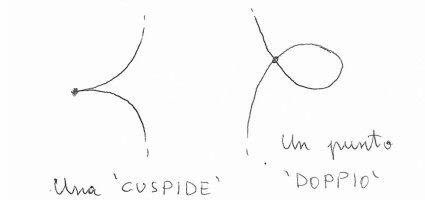
\includegraphics[width=20em]{punti-singolari.jpeg}
\curvegraph{y**2 - x**3 - x**2}{[-2:2]}{[-2:2]}

\textit{Algebricamente}, un punto $p$ zero di $f$ è singolare se $\partial_{x_i}f(p)=0$ per $i=0,\ldots,n$ (ha il differenziale nullo). \notamargine{Se il campo ha caratteristica 0, notare che $\partial_{x_i}f(p) = 0$ per ogni $i$ implica $f(p)=0$ per il \href{https://it.wikipedia.org/wiki/Funzione_omogenea}{teorema di eulero} sulle funzioni omogenee.}


\section{Cubiche, forma di Weierstrass}
Nel caso speciale di $n=2$, $\chr \bbK = 0$ c'è un importante risultato di classificazione delle curve non singolari. 
\notamargine{Una curva si dice non singolare se ogni suo punto è non singolare.} 

Consideriamo curve descritte da
$$ zy^2= ax^3+bx^2z+cxz^2+dz^3 $$
 dove $ax^3+bx^2+cx+d$ è un polinomio senza radici multiple, detta \smallcaps{forma di weierstrass}. Allora è non singolare. Imponiamo infatti le tre equazioni:

%% ESERCIZIO: dimostrare che la forma di weierstrass è non singolare

$$ \left\{ 
\begin{matrix}
&3ax^2&+2bxz&+cz^2 & = & -\partial_{x}f & = 0 \\
&&yz& & = & \partial_{y}f / 2 &= 0 \\
y^2 &-bx^2&-2cx&-3dz^2 & = & \partial_{z}f& = 0 \\
ax^3&+bx^2z&+cxz^2&+dz^3& = & zy^2&
\end{matrix}
\right.$$

Dalla (2) abbiamo due casi:

\begin{itemize}
	\item Se $z=0$ allora (4) dà $x=0$ e dunque $y=0$ dalla (3), assurdo.
	\notamargine{ Siamo nel proiettivo: $x=y=z=0$ non è un punto!} 

	\item Se $y = 0$, $z \neq 0$ allora (4) dà $q(x/z) = 0$ e (1) dà $q'(x/z) = 0$ (dove $q$ è il polinomio di coefficienti $a,b,c,d$). Ma allora $x/z$ sarebbe una radice multipla di $q$, assurdo.  
	\notamargine{Infatti vale il criterio della derivata, cioè un polinomio $p$ ha radici multiple se e solo se $p$ e $p'$ hanno un fattore in comune.}
\end{itemize}

Viceversa, data una curva cubica non singolare, può essere descritta da un polinomio in forma di weierstrass. Algebricamente, per ogni polinomio omogeneo $f$ di grado 3 con differenziale mai nullo, esiste una $L \in \bbP GL_2(\bbK) $ tale che $f \circ L$ (che è ancora un polinomio omogeneo di grado 3) è in forma di Weierstrass. 
\paragraph{IDEA}. Si dimostra che esiste un punto di flesso, e poi si considera una proiettività che manda il punto di flesso nel punto all'infinito. A quel punto, con pochi conti, si arriva alla forma di Weierstrass.
\notamargine{Un punto sulla cubica è di flesso se è un punto non singolare e la tangente ha ordine di contatto $>2$. Notare che nella forma di Weierstrass $(0:1:0)$ è un punto di flesso}

\section{Cubiche, struttura di gruppo}

Sia $\bbK$ algebricamente chiuso. Osserviamo che presi due punti $P,Q$ su una cubica $\gamma$ e tracciata la retta $r$ per $P,Q$, essa interseca $\gamma$ esattamente in un altro punto $R:=P * Q = Q*P$. \notamargine{Vedi il \href{https://en.wikipedia.org/wiki/B\%C3\%A9zout's_theorem}{Teorema di Bezòut}.}

Fissata un'origine $O \in \gamma$, si può dimostrare che l'operazione $(P,Q) \mapsto P \cdot Q = O*(P*Q)$ rende $\gamma$ un gruppo (banalmente) abeliano. Il cambio dell'origine dà luogo a un gruppo isomorfo. Infatti se $O,O'$ sono due origini diverse, detto $O'' = O*O'$, la mappa $P \mapsto O'' * P$ è l'isomorfismo cercato:
\notamargine{Solitamente, nella forma di weierstrass, si prende $O=(0:1:0)$, il punto all'infinito.}
$$ O'' * (P \cdot' Q) = O'' * O'*P*Q = O*P*Q $$
$$ (O''*P) \cdot (O''*Q) = (O*O'')*(P*O'')*Q = O'*O''*P*Q=O*P*Q$$

%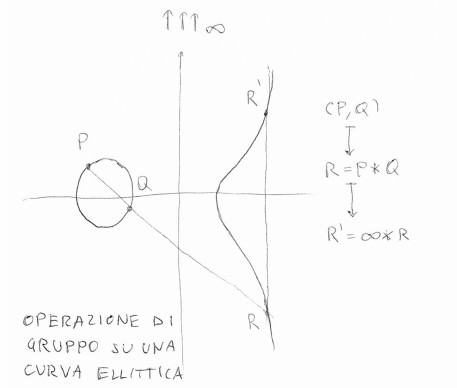
\includegraphics[width=16em]{gruppo-cubica.jpeg}

L'associatività è la proprietà più impegnativa da dimostrare. Vale la pena di notare che l'operazione è una funzione razionale delle coordinate dei punti. 
\section{Funzioni ellittiche, curve ellittiche, reticoli}
C'è una stretta correlazione tra reticoli\notamargine{Per reticoli, dove non diversmaente specificato, intendermo reticoli di rango 2 nel piano complesso}, funzioni ellittiche, curve ellittiche.

Dato un reticolo $L$, saremo in grado di costruire una funzione olomorfa con gruppo dei periodi L detta $\wp_L$.
D'altronde, questa speciale funzione ellittica $\wp_L$ rispetta $\wp_L'(z)^2= f_L(\wp_L(z))$ per un opportuno polinomio di terzo grado $f_L$. Perciò, la funzione $\varphi_L: z \mapsto (\wp_L'(z), \wp_L(z) )$ parametrizza una cubica $E_L$.

\begin{diagram}
 \bbC & \rTo & E_L \\
 \dTo &  \ruTo    & \\
 \bbC/L & &  \\
\end{diagram}
 
\section{Moduli}
Vogliamo cercare ora uno 'spazio dei parametri' per i tori complessi. Conosciamo già una parametrizzazione ridondante: dato un reticolo discreto $L=\omega_1 \bbZ + \omega_2 \bbZ$ possiamo costruire il toro $\bbC / L$ ( e tutti i tori sono definiti così), con $\omega_1, \omega_2$ non paralleli (ossia $\omega_1/\omega_2$ non reale). Cerchiamo ora di eliminare la ridondanza della parametrizzazione, partendo da $\mathcal{A} = \{ (\omega_1, \omega_2) \in \bbC^2: \Im(\omega_1/\omega_2) \neq 0 \} $. 

\begin{enumerate}
\item (orientazione) Anzitutto, a meno di scambiare $\omega_1, \omega_2$, possiamo supporre che $\Im(\omega_1/\omega_2) > 0$: infatti se fosse negativa, $\Im(\omega_2/\omega_1) = -\Im(\omega_1/\omega_2)  > 0$ sarebbe positiva.
\item (riscalamento) Se $\lambda \in \bbC^*$, allora $\bbC/\lambda L  \simeq \bbC/L$ tramite la mappa $z \mapsto \lambda z$ da $C/L$ in $C/\lambda L$. Dunque se $L= \omega_1\bbZ + \omega_2 \bbZ$ con $\Im(\omega_1/\omega_2) > 0$ possiamo considerare $\omega_2^{-1}L= \tau \bbZ + \bbZ $ con $\Im \tau > 0$. Ora il nostro spazio dei parametri perciò è $\mathcal{H} = \{ \tau \in \bbC: \Im \tau > 0 \} \simeq \mathcal{A} / \text{omotetie}$. Se $(\omega_1, \omega_2) \in \mathcal{A}$ indichiamo con $[\omega_1, \omega_2]$ la sua classe di equaivalenza a meno di omotetie, che ha un rappresentante privilegiato $[\omega_1/\omega_2, 1]$ in $\mathcal{H}$.
\item (cambio base) Se $M$ è una matrice 2x2 a coefficienti interi e $L=\omega_1\bbZ + \omega_2\bbZ$ è un reticolo, possiamo considerare il reticolo generato da $M[\omega_1, \omega_2]$ ($M \in End(\bbZ^2) \subset End(\bbC^2)$ agisce sulle coppie di complessi). Visto che le coppie di complessi sono a meno di omotetie, possiamo considerare $M,N \in End(\bbZ^2)$ equivalenti se esiste $\lambda \in \bbC^*$ tale che $\lambda M = N$. Il gruppo delle matrici invertibili a meno di scalari si chiama $\bbP GL_2(\bbZ)$. \notamargine{In realtà, visto che $M,N$ sono a coefficienti interi, $\lambda$ deve essere razionale.} Se $M \in \bbP GL_2(\bbZ)$, allora $M[\omega_1,\omega_2]$ è equivalente a $[\omega_1,\omega_2]$, perciò lo spazio dei parametri ora è $(\mathcal{A}/\text{omotetie})/\bbP GL_2(\bbZ)$.
\item (parametrizzazione esplicita) Così come per ogni classe di equivalenza $[\omega_1, \omega_2]$ a meno di omotetie abbiamo scelto un rappresentante privilegiato $[\tau,1]$, così scegliamo per ogni matrice $[M] \in \bbP GL_2(\bbZ)$ a meno di omotetie un rappresentante privilegiato in $SL_2(\bbQ)$. Infatti $[M*M'] = \mathrm{ Id} $ significa che esiste $\lambda \in \bbC^*$ tale che
$[M]*[M'] = \lambda \mathrm{Id} $. In particolare $\mathrm{det } M$ è invertibile, perciò possiamo scegliere $(\mathrm{det }M)^{-1}M$ equivalente a $M$ e condeterminante 1 ( e ha coefficienti in $\bbQ$). Se prendiamo ora $M \in SL_2(\bbQ)$ di coefficienti $a,b,c,d$ e lo facciamo agire su $[\tau,1]$ otteniamo $\displaystyle [a\tau+b,c\tau+d]= \left [ \frac{a\tau+b}{c \tau + d}, 1 \right ] $ .\notamargine{e si può verificare che  $\frac{a\tau+b}{c \tau + d}$ ha ancora parte immaginaria positiva.} Perciò $SL_2(\bbQ)$ agisce su $\mathcal{H}$ tramite $ M( \tau) = \frac{a \tau+b}{c\tau+d} $, e il nostro spazio dei parametri diventa infine $\mathcal{H} / SL_2(\bbQ)$.
\end{enumerate}

Dimostreremo nelle prossime lezioni che questa parametrizzazione non è più ridondante: se due tori hanno parametri diversi, allora \textit{non} sono biolomorfi. Questo seguirà dalla classificazione esplicita delle funzioni olomorfe tra tori (vedi lezione sulle isogenie).



\chapter{26 Settembre 2016} %TODO: Trovare un titolo.
%TODO: Abbassare le notamargine...

\section{Preliminari ed esempi}
% TODO: definizione giusta di superficie di Riemann: forse è meglio sia direttamente nelle lezioni precedenti.
In questa lezione discuteremo di alcuni esempi di superfici di Riemann, e cominceremo ad introdurre alcuni risultati che ci aiuteranno a classificare specifiche classi di superfici di Riemann a meno di isomorfismo.



\textbf{Esempi di superfici di Riemann compatte:}
\begin{enumerate}
  \item $\bbC$ (o un qualsiasi aperto connesso di $\bbC$). In questo caso l'unica carta è tutto l'insieme, con la mappa di immersione.
  \item La sfera di Riemann $\bbP^1(\bbC)$. $\bbP^1(\bbC)=U_0\cup U_1$ dove $U_0=\{(x_0:x_1)\in \bbP^1(\bbC) | \ x_0\neq 0\}$ e $U_1=\{(x_0:x_1)\in \bbP^1(\bbC) | \ x_1\neq 0\}$, con le mappe $\varphi_0(x_0:x_1)=\frac{x_1}{x_0}$ e $\varphi_1(x_0:x_1)=\frac{x_0}{x_1}$.
  \item Curve algebriche non singolari in $\bbP^2(\bbC)$ ($\{(x:y:z)\in \bbP^2(\bbC) | \ f(x,y,z)=0\}$, dove $f\in \bbC[x,y,z]$ è un polinomio irriducibile. %TODO Dimstrazione.
\end{enumerate}
\notamargine{ACHTUNG! Manca la dimostrazione che le curve algebriche non singolari sono superfici di Riemann.}
\begin{osservazione}
    In $\bbP^2(\bbC)$ vale che ogni curva definita da un polinomio riducibile (che non sia una potenza di un irriducibile) è singolare. Infatti, detto $f(x,y,z)=p(x,y,z)\cdot q(x,y,z)$, se $p$ e $q$ non sono una potenza di uno stesso polinomio irriducibile, deve esistere un punto isolato in $\{p(x,y,z)=0\}\cap\{q(x,y,z)=0\}\subseteq \bbP^2(\bbC)$. In questo punto la curva è formata da due "bracci" che si intersecano, e quindi non è localmente esprimibile come grafico, pertanto necessariamente entrambe le derivate parziali si annullano, dunque è singolare. %TODO qui ci starebbe molto bene un disegnino (magari nelle note).
\end{osservazione}
Durante il corso, vorremmo arrivare a questo teorema:
\begin{teorema}[di Chow]
    Gli esempi precedenti costituiscono tutti gli esempi di superfici di Riemann compatte immerse in $\bbP^2(\bbC)$.
\end{teorema}
\begin{osservazione}
    Una superficie di Riemann meno un numero finito di punti resta una superficie di Riemann. Questo è dovuto al fatto che un aperto connesso di $\bbC$ meno un punto resta un aperto connesso.
\end{osservazione}
%TODO Curve algebriche singolari meno i punti singolari


\textbf{Esempi di superfici di Riemann non compatte:}
\begin{enumerate} %TODO Far partire l'indice da 4
  \item $\bbC/\bbZ$.
  \item $\bbC/L$, dove $L$ è un reticolo (discreto) di rango 2.
\end{enumerate}
\begin{proof} \textit{(che sono superfici di Riemann)}
    Dimostriamo solo che $\bbC/\bbZ$ lo è, la dimostrazione per $\bbC/L$ è analoga. Considero $\pi:\bbC\rightarrow\bbC/\bbZ$ la proiezione al quoziente, e $Y:=\{z\in\bbC|\ 0\leq Re(z)<1\}$ una striscia verticale di rappresentanti. Ricopro $Y\subseteq\bbC$ con dischi $D_\alpha$ (aperti) di raggio $1$ (in modo che $D_\alpha$ non contenga mai due punti che al quoziente sono uguali). Si osserva facilmente che $\pi_{|D_\alpha}$ è un omeomorfismo, scegliamo $\varphi_\alpha=\pi_{|D_\alpha}^{-1}$, si verifica facilmente soddisfare le proprietà richieste dalla definizione.

    Nel caso del reticolo di rango $2$, la dimostrazione si fa prendendo come $Y$ un parallelogrammo, e raggio dei dischi abbastanza piccolo da impedire che ci possano essere due punti equivalenti nello stesso disco.
\end{proof}

\begin{definizione}
Siano $X$ e $Y$ due superfici di Riemann, $x_0\in X$, $y_0=f(x_0)$. $f:X\rightarrow Y$ si dice olomorfa in $x_0$ se esiste un intorno $A$ di $x_0$ tale che $A\subseteq U_\alpha$ e detto $V_\beta$ un aperto del ricoprimento di $Y$ che contiene $y_0$, vale che $\psi_\beta \circ f \circ \varphi_\alpha^{-1}: \varphi_\alpha(A)\rightarrow \bbC$ è una funzione olomorfa.
\end{definizione}

\notamargine{Più precisamente si dovrebbe richiedere che per OGNI $U_\alpha$ e $V_\beta$ che contengono $x_0$ o $y_0$ valga quella proprietà, ma questo è equivalente alla definizione data per la proprietà di compatibilità sulle intersezioni delle $\varphi_\alpha$ e $\psi_\beta$.}

\begin{definizione}
Due superfici di Riemann $X$ e $Y$ si dicono isomorfe (o conformemente equivalenti) se esiste $f:X\rightarrow Y$ invertibile, olomorfa con inversa olomorfa.
\end{definizione}

\notamargine{Una tale $f$ viene definita biolomorfismo.}

\begin{osservazione}
Sia $X$ una superficie di Riemann, $Y$ uno spazio topologico, $f:X\rightarrow Y$ un omeomorfismo. Allora posso trasportare su $Y$ la struttura complessa di $X$, ricoprendolo con aperti $V_\alpha=f(U_\alpha)$ e mappe $\psi_\alpha=\varphi_\alpha \circ f^{-1}_{|f(U_\alpha)}:f(U_\alpha)\rightarrow\bbC$
\end{osservazione}

\notamargine{Con questa struttura di varietà, chiaramente $Y$ è isomorfo ad $X$}

\section{Classificazione delle superfici di Riemann}
Cerchiamo di muoverci verso un risultato riguardo la classificazione delle superfici di Riemann. Lo schema con cui affronteremo il problema consiste nel considerare un rivestimento universale della superficie di Riemann e cercare esprimere la superficie di partenza come quoziente dello spazio rivestente per un gruppo di automorfismi. In questo modo sposteremo il problema sullo studio dei sottogruppi del gruppo di automorfismi di (speriamo poche) superfici fissate.
\begin{osservazione}
Sia $X$ una superficie di Riemann, se $\pi:Y\rightarrow X$ è un rivestimento, allora $Y$ è in modo naturale una superficie di Riemann.
\end{osservazione} 
\begin{proof}[Idea della dimostrazione]
È possibile fare un raffinamento degli $U_\alpha\subseteq X$ in modo da renderli "compatibili" con gli aperti banalizzanti del rivestimento (per esempio, posso considerare le intersezioni con essi). In questo modo, avendo gli $U_\alpha$ inclusi in un aperto banalizzante, è possibile "tirarli su" sullo spazio ricoprente, e definire le $psi_\alpha=\phi_alpha \circ \pi$. La verifica che sono rispettate le proprietà della definizione è banale.
\end{proof}
Enunciamo adesso il risultato chiave che ci permetterà di procedere con la classificazione:
\begin{teorema}[di Riemann]
Ogni superficie di Riemann semplicemente connessa è biolomorfa ad uno dei seguenti tre modelli:
\begin{enumerate}
  \item La sfera di Riemann $\bbP^1(\bbC)=:\widehat{\bbC}$.
  \item Il piano complesso $\bbC$.
  \item Il disco di Poincaré $D$.
\end{enumerate}
\end{teorema} 
\begin{proof}
La dimostrazione non verrà trattata in questo corso a causa dell'eccessiva difficoltà.
Nella prossima lezione vedremo che queste tre superfici non sono biolomorfe (è una conseguenza del teorema di Liouville.
\end{proof}
\begin{osservazione}
Sia $\pi:\widetilde{X}\rightarrow X$ un rivestimento universale, $x_0\in X$. Allora la fibra $\pi^{-1}(x_0)$ è discreta in $\widetilde{X}$, ed esiste un gruppo di omeomorfismi di $\widetilde{X}$ che preserva le fibre ed agisce in modo transitivo su di esse. Chiamato $G$ tale gruppo, si ha che $X \simeq \widetilde{X}/G$.
\end{osservazione}
\begin{definizione}
Sia $G$ un gruppo che agisce su uno spazio topologico $X$. L'azione di $G$ si dice \textit{propriamente discontinua} se per ogni compatto $K\subseteq X$ esiste solo un numero finito di elementi di $G$ tali che $g(K)\cap K =\varnothing$.
\end{definizione}
\begin{fatto}
Sia $X$ una superficie di Riemann con un gruppo di automorfismi olomorfi $G<Aut(X)$. Allora $X/G$ è in modo naturale una superficie di Riemann se valgono le seguenti due proprietà:
\begin{enumerate}
  \item L'azione di $G$ su $X$ è propriamente discontinua.
  \item Gli elementi di $G\setminus\{\Id\}$ agiscono senza punti fissi.
\end{enumerate}
\end{fatto}
\notamargine{Se non sono soddisfatte le due condizioni, allora $X\rightarrow X/G$ non è nemmeno un rivestimento, a prescindere dalla struttura complessa.} 
\chapter{28/09/16 - Non ho ancora ben capito su cos'è questa lezione}
\justify
%Balbo sappi che ti sto odiando per tutti quei comandi definiti un po' in modo libertino.

\newthought{Eravamo rimasti} a questo enunciato:
\begin{teorema}
	Sia $M$ una varietà, e sia $G$ un gruppo di omeomorfismi di $M$.
 	Allora la proiezione al quoziente $p:M\rar \quoziente{M}{G}$ è un rivestimento se e solo se $G$ agisce in modo propriamente discontinuo.
\end{teorema}
\notamargine{$\Rar$ è ovvia e $\Lar$ sta sul Manetti}

Qui, seguendo il Manetti, intendo che $G$ agisce in modo propriamente discontinuo se $\forall\ x\in X\ \exists\ U\subset X$ aperto tale che $\forall\ g\in G, g(U)\cap U=\emptyset$. 

Se ho qualche piccola ipotesi su X (essere varietà basta e avanza), questo è equivalente a chiedere che $G$ sia libero, cioè che $\forall\ x \in X, \forall\ g\in G, g(x)\neq X$, e che $\forall\ K \subset X$ compatto, $g(K)\cap K \neq \emptyset$ solo per un numero finito di $g$.
\notamargine{$\Lar$ sta sul Manetti, $\Rar$ ha una parte ovvia e una che usa compattezza per successioni}
%Nota: Capire perché le note a margine sono impaginate schifo

A questo aggiungo un altro teorema:

\begin{teorema} \label{rivuniv}
 	Sia $p:E\rar X$ un rivestimento universale. Allora esiste $G$ gruppo di omeomorfismi di $E$ propriamente discontinuo tale che $X\isom\quoziente{E}{G}$.
\end{teorema}
\notamargine{Ricordo che $p:E\rar X$ rivestimento si dice universale se $E$ è semplicemente connesso}
\notamargine{Anche qui la dimostrazione sta sul Manetti, in posti a caso}

Adesso, sia $X$ una \sdR, e sia $\pi:X\rar\ot X$ il suo rivestimento universale (che ricordo essere unico a meno di omeomorfismi). Attraverso $\pi$, $\ot X$ eredita una struttura di \sdR\ da quella di $X$.

Infatti, prendendo un raffinamento $U_\alpha$ del ricoprimento su $X$ dato dalla definizione di \sdR, posso pensare che gli $U_\alpha$ sono aperti banalizzanti per $\pi$, ottenendo dunque un ricoprimento su $\ot X$ dato dagli insiemi $V_\alpha^r$, dove $\pi^{-1}(U_\alpha)=\sqcup_r V_\alpha^r$, in cui le carte locali sono le funzioni $\phi_\alpha^r=\phi_\alpha\circ\pi$. Il fatto che i cambi di carta siano olomorfi su $\ot X$ discende dal fatto che lo siano su $X$.

Ora, per il teorema \ref{rivuniv}, esiste $G$ fatto nel modo giusto tale che $\quoziente{\ot X}{G}\isom X$.
\begin{lemma}
 	%Balbo ti odio, perché non potevi mettere tra i similteoremi anche proposizione?
 	Sia $g\in G$. Allora $g$ è olomorfa come applicazione tra \sdR.
\end{lemma}
\begin{proof}
 	Osservo che ovviamente $g \in \mbox{Aut}\left(\quoziente{\ot X}{X}\right)$, cioè $g$ è un automorfismo di rivestimento (in inglese \emph{deck transformation}), cioè $g$ preserva le fibre. Questa condizione si può scrivere anche come $\pi\circ g=\pi$.
 	
 	Sia ora $x\in \ot X$. Sia $V_\alpha^r$ uno degli aperti della condizione di \sdR\ tale che $x\in V_\alpha^r$, e sia $\phi_\alpha^r$ la sua carta locale. Si ha $g(x)\in V_\alpha^s$ per un qualche $s$, e dunque bisogna dimostrare $\phi_\alpha^s\circ g\circ (\phi_\alpha^r)^{-1}$ olomorfa in $\phi_\alpha^r(x)$. Ma questa funzione si può scrivere anche come $\phi_\alpha\circ\pi\circ g\circ \pi^{-1}\circ \phi_\alpha^{-1}$, che poiché $g$ è automorfismo di rivestimento è uguale a $\phi_\alpha\circ\pi\circ\pi^{-1}\circ\phi_\alpha^{-1}=id$. Poiché l'identità è olomorfa, abbiamo dimostrato che $g$ è olomorfa.
\end{proof}
\notamargine{$\pi^{-1}$ dovrebbe presentare un pedice che si riferisce al fatto che ha codominio $V_\alpha^r$, ma non l'ho ritenuto fondamentale}

Ora, per classificare le \sdR\ posso dunque studiare tutti i quozienti opportuni di \sdR\ semplicemente connesse. Per il Teorema di Riemann, queste sono solo $\bbP_1(\bbC)=\oc \bbC, \bbC, \cD\isom\cH$, dove su quest'ultimo ho la struttura complessa data dall'inclusione.

Dunque il prossimo passo è classificare i gruppi di isomorfismi propriamente discontinui e olomorfi delle tre \sdR\ semplicemente connesse.

\newthought{Ora iniziano} cose di cui non ho esattamente capito il senso, per ora.

\begin{definizione}
	Sia $A\subset\bbC$. Una funzione $f:A\rar\bbC$ si dice \emph{algebrica} se $\exists\ p\in\bbC[x,y], p\neq0 \tc p(x,f(x))=0\ \forall\ x\in A$.
\end{definizione}
%qui vorrei un ambiente esercizio
\begin{lemma}
 	$f(x)=e^x$ non è una funzione algebrica.
\end{lemma}
\begin{proof}
 	Lasciata come esercizio
\end{proof}

Ora si sta parlando di rivestimenti indotti da funzioni algebriche.

Per esempio, consideriamo la funzione $p(t)=t^2, p:\bbC\rar\bbC$. Questa funzione non è bigettiva, dunque non ha un'inversa globale, ma comunque localmente ha un'inversa. Devo però effettuare una scelta per ottenere questa inversa locale, in paricolare la scelta del segno. Inoltre vorrei che quest'inversa locale sia quantomeno continua. Si dimostra però che in ogni intorno di $0$ non esiste nessuna funzione continua tale che $f(x)^2=x$ per ogni $x$.

Questo si può vedere tramite i rivestimenti. Infatti la funzione $p(t)$ non è un rivestimento di $\bbC$ su sè stesso, proprio perché l'immagine inversa di ogni intorno di $0$ non è mai omeomorfa all'intorno tramite la mappa $p$.

Se però considero $p:\bbC^*\rar\bbC^*$, ho che questo è un rivestimento di grado $2$, e pertanto, poiché $\bbC^*$ è connesso, non può avere sezioni globali, ma solamente sezioni locali.
\notamargine{Se $p:E\rar X$ è rivestimento, una sua sezione $\phi$ è una mappa continua da $U\subset X$ a $E$ 


È facile osservare che $z\rar-z$ è un automorfismo di rivestimento per 






\chapter{3 Ottobre 2016 - Automorfismi delle superfici di Riemann semplicemente connesse}
\justify

\begin{definizione}[Superficie di Riemann (speriamo)]
Si dice superficie di Riemann una varietà complessa connessa di dimensione $1$, cioè uno spazio topologico di Hausdorff (T2)
connesso tale che ogni suo punto abbia un intorno $U_\alpha$ omeomorfo a un aperto $V_\alpha$ di $\mathbb{C}$
tramite l'omeomorfismo $\varphi_\alpha$, e che per ogni $\alpha$ e $\beta$ valga che $\varphi_\beta \circ {\varphi_\alpha}^{-1}$
sia una funzione olomorfa in $\varphi_\alpha \left( U_\alpha \cap U_\beta \right)$.
\end{definizione}

\begin{osservazione}
La richiesta di essere T2 non si deduce dalle altre condizioni. Infatti se consideriamo il "disco con due origini",
cioè il quoziente $S/\!\!\sim$ dove $S=D\times\{0\} \cup D\times\{1\}$ e $x\sim y \Longleftrightarrow x=y$ oppure $x=(u,i),\ y=(u,j)$ con $\{i,j\}=\{0,1\}$,
si osserva che ogni punto ha un intorno omeomorfo a un aperto di $\mathbb{C}$ ma $(0,0)$ e $(0,1)$ non hanno intorni disgiunti.
\end{osservazione}

\begin{esercizio}
$S/\!\!\sim$ è semplicemente connessa.
\end{esercizio}

Determiniamo ora i gruppi degli automorfismi delle superfici di Riemann semplicemente
connesse: $\mathbb{P}^1(\mathbb{C})$, $\mathbb{C}$, $D$.


\section{Automorfismi di $\mathbb{P}^1(\mathbb{C})=\hat{\mathbb{C}}$}
Vogliamo dimostrare che $Aut( \hat{\mathbb{C}} )= \mathbb{P}GL_2 (\mathbb{C} )=\left\{z\mapsto \displaystyle{\frac{az+b}{cz+d}} \ ,\ \  ad\neq bc\right\}$

\begin{definizione}[Grado di una funzione razionale]
Si definisce grado di $\frac{p(x)}{q(x)}$ il massimo tra i gradi di $p(x)$ e $q(x)$.
Si può osservare che, come per i polinomi, il grado è il numero di controimmagini di ogni punto contate con molteplicità.
\end{definizione}

\begin{osservazione}
$\varphi \in Aut( \hat{\mathbb{C}} ) \Longrightarrow deg(\varphi )=1$, perché deve essere un omeomorfismo e quindi è iniettivo. 
\end{osservazione}


\begin{lemma}
$G= \mathbb{P}GL_2 (\mathbb{C} )$ è triplamente transitivo, cioè date due terne
$(x_1 , x_2 , x_3 ) \in \hat{\mathbb{C}}^3$ e $(y_1 , y_2 , y_3 ) \in \hat{\mathbb{C}}^3$
con $x_i \neq x_j$ e $y_i \neq y_j$ se $i \neq j$, $\exists ! g \in G$ t.c. $g(x_i )=y_i$ per $i=1,2,3$.
\end{lemma}
\begin{proof}
Basta farlo per $(x_1 , x_2 , x_3 ) = (0,1,\infty )$ e $y_i \neq \infty$, a meno di comporre con qualche elemento di $G$.
Devo quindi trovare $a,b,c,d \in \mathbb{C}$ tali che:
$$
\left\{
\begin{array}{l}
\medskip
\displaystyle{\frac{0a+b}{0c+d}=\frac{b}{d}=y_1} \\
\medskip
\displaystyle{\frac{1a+b}{1c+d}=\frac{a+b}{c+d}=y_2} \\
\displaystyle{\frac{\infty a+b}{\infty c+d}=\frac{a}{c}=y_3}
\end{array}
\right.
$$
da cui sostituendo si ottiene $y_3 c + y_1 d=y_2 (c+d)$ e si vede che, se $y_i \neq y_j$ quando $i \neq j$, esistono $c$ e $d$ con $c+d \neq 0$ che risolvono l'equazione.

Resta quindi da mostrare l'unicità. Per farlo basta verificare che l'unico elemento di $G$ che fissa una data terna
(prendiamo ancora $(0,1,\infty )$) è l'identità. Imponiamo quindi che:
$$
\left\{
\begin{array}{l}
\medskip
\displaystyle{\frac{0a+b}{0c+d}=\frac{b}{d}=0} \\
\medskip
\displaystyle{\frac{1a+b}{1c+d}=\frac{a+b}{c+d}=1} \\
\displaystyle{\frac{\infty a+b}{\infty c+d}=\frac{a}{c}= \infty}
\end{array}
\right.
$$
da cui si ricava subito $a=d=1$, $b=0$ e $c=0$, cioè la trasformazione considerata è l'identità.
\end{proof}

\begin{esercizio}
I sottogruppi finiti di $\mathbb{P}GL_2 (\mathbb{C} )$ sono:
\begin{itemize}
\item Tutti i gruppi ciclici
\item Tutti gruppi diedrali
\item $S_4$ e $A_5$
\end{itemize}
\end{esercizio}


\begin{proposizione}
$Aut (\hat{\mathbb{C}} ) = G = \mathbb{P}GL_2 (\mathbb{C} )$
\end{proposizione}
\begin{proof}
Sia $\varphi \in Aut (\hat{\mathbb{C}} )$. Sappiamo già che $Aut (\hat{\mathbb{C}} ) \subseteq G$.
Quindi, essendo $G$ triplamente transitivo, possiamo assumere $\varphi( \infty ) = \infty$.
Ora osserivamo che, essendo $\varphi$ un automorfismo olomorfo, detto $D=D(0,1)$, $\varphi (D)$ conterrà
un certo disco $D_1$. Quindi $\varphi$ non può avere una sigolarità essenziale all'infinito poiché in tal caso,
per il teorema di Weierstrass, dovrebbe assumere valori densi in $\mathbb{C}$ in ogni intorno di $\infty$
e quindi anche valori in $D_1$ contraddicendo l'iniettività di $\varphi$.
Allora $\varphi$ ha un polo all'infinito ed è olomorfa su $\mathbb{C}$, quindi deve essere un polinomio (basta considerare la sua espansione in serie) e,
essendo anche iniettiva, deve avere grado $1$. Quindi $\varphi \in G$.
\end{proof}


\section{Automorfismi di $\mathbb{C}$}
Studiamo ora gli automorfismi olomorfi di $\mathbb{C}$.
Sia $g \in Aut(\mathbb{C})$. Allora, come prima, per il teorema di Weierstrass $g$ ha un polo all'$\infty$,
quindi è un polinomio e ha grado $1$ per iniettività. Quindi
$Aut(\mathbb{C} )= \left\{ z\mapsto az+b \right\} = Stab_{\mathbb{P} GL_2 (\mathbb{C})} (\infty )$.


\section{Automorfismi di $D$}
\begin{definizione}[Trasformazioni di Möbius]
Si chiamano Trasformazioni di Möbius le trasformazioni del tipo $z\mapsto c \displaystyle{\frac{z-a}{1- \bar{a}z}}$ con $|c|=1$ e $a \in D$.
\end{definizione}

\notamargine{A volte invece si chiamano così tutte le trasformazioni di $\mathbb{P} GL_2 (\mathbb{C})$}
%Esce troppo in alto. Come faccio a metterla vicino alla definizione?

\begin{esercizio}
Le trasformazioni di Möbius sono un sottogruppo di $\mathbb{P} GL_2 (\mathbb{C})$.
\end{esercizio}

\begin{osservazione}
Le trasformazioni di Möbius mandano D in se stesso. Infatti: 
$$\left|c \frac{z-a}{1- \bar{a}z} \right|= 1 \frac{(z-a)(\bar{z}-\bar{a})}{(1- \bar{a}z)({1- a\bar{z}})}=
\frac{|z|^2 + |a|^2 - 2Re(a \bar{z})}{1+ |a|^2 |z|^2 - 2Re(a \bar{z})} <1
\Longleftrightarrow \left( 1-|z|^2 \right) \left( 1-|a|^2 \right) >0$$
Questa è vera $\forall z \in D$.
\end{osservazione}

\begin{osservazione}
Il gruppo delle Trasformazioni di Möbius G ha dimensione topologica 3 (è come $S^1 \times D$),
quindi ci aspettiamo che sia transitivo ma non doppiamente transitivo.
\end{osservazione}

\begin{lemma}
$G= \left \{ z \mapsto \displaystyle{c \frac{z-a}{1- \bar{a}z}} \right \}$ è transitivo.
\end{lemma}
\begin{proof}
È evidente che si può mandare $0$ in qualsiasi punto di $D$ (anche ponendo $c=1$).
\end{proof}

\begin{osservazione}
$Stab_G (0) = \{z \mapsto cz \}$ cioè tutte e sole le rotazioni.
\end{osservazione}

\begin{lemma}[di Schwarz]
Sia $f:D\rightarrow D$ una funzione olomorfa tale che $f(0)=0$. 
Allora $|f(z)| \leq |z|\ \ \forall z \in D$ e $f'(0) \leq 1$. Inoltre, se vale un'uguaglianza, $f$ è una rotazione.
\end{lemma}
\begin{proof}
$f(0)=0 \Rightarrow \frac{f(z)}{z}$ è olomorfa in $D$. Detto $D_r$ il disco di raggio $r$,
per il principio del massimo modulo si ha che, per $z \in D_r$
$$\left| \frac{f(z)}{z} \right| \leq \sup_{|z|=r} \left| \frac{f(z)}{z} \right| \leq \frac{1}{r} \ \  \forall r \in (0,1)
\Longrightarrow \left| \frac{f(z)}{z} \right| \leq 1 \ \ \forall z \in D$$
Facendo tendere $z$ a $0$ si ottiene anche la tesi sulla derivata.
Infine, se si verifica un'uguaglianza, sempre per il principio del massimo modulo risulta che
$\left| \frac{f(z)}{z} \right|$ è costante in $D$, quindi $f$ è una rotazione.
\end{proof}

\begin{proposizione}
$Aut(D)=G$
\end{proposizione}
\begin{proof}
Sappiamo che $Aut(D) \supseteq G$. Sia quindi $\varphi \in Aut(D)$. Essendo $G$ transitivo posso supporre che $\varphi(0)=0$.
Sia $\psi$ l'inversa di $\varphi$. $\psi (0)=0$. Quindi
$\psi (\varphi (z))=z \stackrel{deriviamo}{\Longrightarrow} \psi ' (\varphi (z)) \varphi '(z) =1 \Rightarrow \psi'(0) \varphi'(0) =1$
Ma per il lemma di Schwarz $|\psi'(0)| \leq 1$ e $|\varphi'(0)| \leq 1|$. Quindi $|\varphi'(0)|=1$ e, sempre per il lemma di Schwarz,
$\varphi$ è una rotazione e quindi appartiene a $G$. 
\end{proof}

\subsection {$D \simeq \mathcal{H}$}

Vediamo ora che il disco $D$ è biolomorfo al semipiano $\mathcal{H} = \left \{ z \in \mathbb{C} | \ Im (z)>0 \right \}$
Presi $w \in \mathcal{h}$ e $z \in D$, consideriamo le mappe:
$$w \mapsto z=\frac{i-w}{i+w} \qquad z \mapsto w= i\frac{1-z}{1+z}$$
Si può verificare sono una l'inversa dell'altra e che sono effettivamente omeomorfismi tra $\mathcal{H}$ e $D$.
Quindi $D \simeq \mathcal{H}$ come superfici di Riemann.

Questo ci permette anche di determinare che $Aut( \mathcal{H}) = \left \{ z \mapsto \displaystyle{\frac{az+b}{cz+d}} \ | \ ad>bc \right \}$

Ora quindi dovremo capire quali sottgruppi di $Aut (\hat{\mathbb{C}})$, $Aut(\mathbb{C})$ e $Aut(D)$ agiscono in modo propriamente discontinuo
e non hanno punti fissi, per classificare le superfici di Riemann.
\thislesson{5 Ottobre 2016}{Sottogruppi discreti}

La scorsa lezione abbiamo determinato i gruppi di automorfismi complessi delle tre superfici di Riemann:
$$
\hat{\bbC},\qquad \bbC, \qquad \mathbb{D}.
$$
Ricordiamo poi il fondamentale
\begin{teorema}[Riemann] Una superficie di Riemman semplicemente connessa è biolomorfa ad una tra:
$\hat{\bbC},\ \bbC, \ \mathbb{D}. $
\end{teorema}
Sappiamo che dunque una generica superficie di Riemann $X$ avrà un rivestimento universale $\tilde{X}$, che dovrà essere uno dei tre precedenti e che $X$ puo' essere ricostruita quozientado $\sfrac{\tilde{X}}{G}$ dove $G<\Aut(\tilde{X})$ è un gruppo che agisce in maniera propriamente discontinua e senza punti fissi.\\
L' idea ora è che sappiamo chi è $\tilde{X}$ e chi sono i suoi automorfismi, quindi se riusciamo a determinare i sottogruppi con le proprietà richieste determiniamo, a ritroso, tutte le possibili superfici di Riemann $X$.\\

Richiamiamo quindi delle definizioni classiche.

\begin{definizione}[Successione esatta corta.] In generale una catena di morfismi tra oggetti algebrici di questo tipo:
$$
A\xrightarrow{\alpha}B\xrightarrow{\beta}C\rightarrow 0
$$
si dice {\it esatta} se $\Im{\alpha}=\Ker{\beta}$.\\
In particolare se abbiamo una sequenza del tipo
$$
0\rightarrow A\xrightarrow{\alpha}B\xrightarrow{\beta}C \rightarrow 0
$$ 
che è esatta in ogni punto allora siamo in presenza di una {\it successione esatta corta}.
\end{definizione}
E' opportuno osservare che le successioni esatte corte sono caratterizzate dalle proprietà:
$$
\Ker \alpha =0;\ \ \Im \alpha =\Ker \beta,\ \ \Im \beta =C.
$$
La definizione è generale ma a noi interesseranno essenzialmente morfismi di gruppi.
Nella pratica le successioni esatte corte danno informazioni sul gruppo centrale se si conoscono quelli laterali: un esempio ci è dato dai prodotti semidiretti:
\begin{fatto}
Sia data una successione esatta corta di gruppi:
$$
0\rightarrow A\xrightarrow{j}B\xrightarrow{\pi}C \rightarrow 0
$$
E supponiamo esista $\sigma:C\rightarrow B$ morfismo tale che:
$$
\pi\circ \sigma=\Id_{\, C} 
$$
cioè esista  una {\it sezione} di $\pi$. Allora $B=A\rtimes_\psi C$ dove $\psi:C
\rightarrow \Aut A$ è il coniugio.
\end{fatto}
\notamargine{Basta scrivere a mano un generico elemento di $B$ come prodotto di uno di $C$ tramite $\sigma$ e uno di $A$ tramite $j$ e evrificare l' unicità. L' operazione poi viene da sè.}
La dimostrazione è lasciata come esercizio.

Nel nostro contesto abbiamo questa interessante successione esatta corta:
$$
0\rightarrow\ (\bbC,+)\ \xrightarrow{j}\ (\Aut{\bbC},\circ)\ \xrightarrow{\pi}\ (\bbC^*,\cdot)\  \rightarrow\ 0
$$
che ha anche una sezione $\sigma$. Le mappe sono definite in maniera abbastanza costretta:
$$
j(w)=(z\mapsto z+w),\qquad \pi(z\mapsto az+b)=a,\qquad \sigma(a)=(z\mapsto az).
$$
\begin{esercizio}
Un sottogruppo finito di $\Aut{\bbC}$ è ciclico.
\end{esercizio}
\notamargine{Non può contenere traslazioni...}
Supponiamo ora di avere una superficie di Riemann $X$ con rivestimento universale $\tilde X$.\\ 
Cerchiamo i sottogruppi $G$ di $\Aut{\tilde{X}}$ tali che:
\begin{itemize}
\item[(i)] l' azione di $G$ su $\tilde{X}$ sia propriamente discontinua;
\item[(ii)] gli elementi di $G\setminus\{\Id\}$ agiscono senza punti fissi.
\end{itemize}
E' opportuno premettere dei lemmi generali, dopo aver osservato che in ognuno dei tre casi $\Aut{\tilde{X}}$ è un gruppo topologico metrico.
\begin{lemma}Sia $\tilde G$ un gruppo topologico metrico e $G$ un suo sottogruppo; allora si equivalgono:
\begin{itemize}
\item[(a)] $G$ è discreto in $\tilde G$;
\item[(b)] l' identità è isolata in $G$;
\item[(c)] $G$ non ha punti di accumulazione in $\tilde G$.
\end{itemize}
\end{lemma}

Passiamo ora alla classificazione.

{\it Primo caso: $X$ sferica i.e. $\tilde {X}=\hat{\bbC}$.} Questo caso è triviale, infatti se $g\in\Aut{\hat{\bbC}}=PGL_2(\bbC)$ la condizione $(ii)$ è soddisfatta solo da $g=\Id$:
$$
g(z)=\frac{az+b}{cz+d}=z\ \Leftrightarrow\ cz^2+(d-a)z-b=0
$$
basta fare i casi e ricordarsi di considerare anche $z=\infty$ per accorgersi che questa equazione ha sempre soluzioni in $\hat{\bbC}$.

{\it Secondo caso: $X$ euclidea i.e. $\tilde{X}=\bbC$.} Questo caso è più interessante. Ricordiamo prima di tutto che gli automorfismi di $\bbC$ sono tutte e sole le affinità:
$$
z\mapsto az+b,\ \ a\in\bbC^*,\ b\in \bbC.
$$
Questa rappresentazione ci permette di mettere una metrica su $\Aut{\bbC}$ identificando i suoi elementi con coppie di numeri complessi, con la seconda coordinata non nulla:
$$
z\mapsto az+b\ \ \leftrightarrow\  (a,b).
$$
Osserviamo che se vogliamo che valga la proprietà (ii) dobbiamo richiedere $a=1$. Questo forza $G$ ad essere un sottogruppo di traslazioni.\\
Vediamo ora che necessariamente l' identità di $G$ è isolata: ragionando per assurdo troveremmo infiniti elementi distinti $\{ g_k=(1,b_k) \}\in G$ tali che:
$$
g_k=(1,b_k)\rightarrow (1,0)=\Id\ \ \ \mbox{ se } k \rightarrow \infty,
$$  
ma allora per ogni aperto non vuoto $U\subseteq \bbC$ si avrebbe definitivamente in $k$ che $g_k(U)\cap U\neq \emptyset$ per la definizione di limite.\\
Per il Lemma 4 dunque si ha che $G$ è discreto.

Consideriamo ora $V_G$ lo span su $\bbR$ di $G$ e separiamo i casi a secondo della sua dimensione reale. Se ha dimensione zero si tratta del gruppo banale, se ha dimensione 1 invece possiamo identificarlo, passando in coordinate, con un sottogruppo additivo discreto di $\bbR$. Con un principio variazionale vediamo che la struttura di tali gruppi è triviale. Consideriamo infatti $g_0$ il
$$
\inf\{g>0\ :\ g\in G\}
$$
di sicuro $g_0>0$ perchè l' identità è isolata. Vorremmo mostrare che $g_0\in G$, per farlo basta ragionare per assurdo e produrre una successione di elementi $\{g_n\}\subseteq G $ che tendono a $g_0$; allora si avrebbe che $g_m-g_n$ (che sta in $G$) si accumula su $0$, assurdo.\\
Dividendo ora con resto un qualsiasi altro elemento di $g'\in G$ per $g_0$ otteniamo che:
$$
g'=k\cdot g+q,\ \ k\in \bbZ,\ \ 0\leq q <g
$$ 
ma allora per minimalità $q=0$ il che implica $G\subseteq \bbZ g_0$ e l' altra inclusione era ovvia.

Rimane il caso in cui la dimensione reale di $V_G$ sia 2. In questo caso esistono $\omega_1,\omega_2$ numeri complessi linearmente indipendenti su $\bbR$ tali che:
$$
G=\bbZ\, \omega_1+\bbZ\, \omega_2.
$$
la dimostrazione è una immediata conseguenza del seguente teorema.

\begin{teorema}Sia $G$ un sottogruppo discreto di $(\bbR^n,+)$. Allora esiste un naturale $d\leq n$ e $d$ vettori di $\bbR^n$, $g_1,\ldots,g_d$ linearmente indipendenti tali che:
$$
G=\bbZ\ g_1+\ldots+\bbZ\ g_d
$$
dove la somma, in effetti, è diretta.
\end{teorema}
\begin{proof}
Procediamo per induzione sulla dimensione di $V_G$, osservando che i passi base $d=0,1$ sono stati fatti nella proposizione precedente. Supponiamo quindi $\Dim{V_G}>1$ e prendiamo $g_0$ il suo elemento nonidentico di minima norma; decomponiamo ora:
$$
V_G=\bbR g_0\ \oplus\  W\ \mbox{ e la rispettiva projezione}\ \pi:V_G\rightarrow W.
$$
\notamargine{Esiste perchè... rielaborare la dimostrazione precedente.}
Osserviamo che su $\Gamma:=\pi(G)\subseteq W$ abbiamo canonicamente una struttura di gruppo.\\
Dimostriamo che $\Gamma$ è discreto, mostrando che la sua identità (che è la stessa di prima) è isolata. Sia $\{\gamma_k=\pi(g_k)\}\subseteq W\setminus\{0\}$ successione tale che $\gamma_k\rightarrow 0$, allora possiamo decomporre ogni $g_k$ così:
$$
g_k=\gamma_k+\lambda_k\, g_0=\gamma_k+q(k)\cdot\, g_0+\delta_k\, g_0,
$$
$$
q(k)\in\bbZ,\ \ 0\leq \delta_k<1
$$
dove nell'ultimo passaggio abbiamo diviso con resto $\lambda_k$ per $|g_0|$. Dunque abbiamo una successione di elementi di $G$ limitata dentro $\bbR^n$:
$$
|g_k-q(k)\cdot g_0| \leq |\gamma_k|+|g_0|
$$
che per discretezza può essere composta solo da un numero finito di elementi, assurdo.
\notamargine{Altrimenti ne estraggo di infiniti distinti, riestraggo per far convergere, considero le differenze che stanno in G e tendono a $0$. Assurdo ché 0 è isolato.}

(Da questo punto dimenticate chi sono i $g_i$ ed i $\gamma_i$ e ne definiamo di nuovi)
A questo punto uso l'ipotesi induttiva su $\Gamma$ e ne produco una $\bbZ$-base come reticolo $\{\gamma_1, \ldots, \gamma_{d-1}\}$.
Inoltre prendiamo $\gamma_0$ come generatore della proiezione su $\bbR g_0$.
A questo punto è ovvio che la famiglia (pensata immersa in $V_G$)
$$
\{\gamma_0,\gamma_1,\ldots,\gamma_{d-1}\}
$$ 
contiene il reticolo $G$, ovvero $G \sqsubseteq \bbZ \gamma_0 + \bbZ \gamma_1 + \ldots + \bbZ \gamma_{d-1}$.

A questo punto usando Nakayama (o il teorema dei gruppi abeliani finitamente generati) si ottiene che $G$ ha dimensione finita (e $\le d$).

Mostriamo che è fatta di vettori linearmente indipendenti addirittura su $\bbR$:
$$
0=\mu_0\, g_0+\mu_1\, g_1+\ldots+\mu_{d-1}\, g_{d-1}
$$
projettando con $\pi$ su $W$ e usando l' ipotesi di lineare indipendenza sui $\{\gamma_i\}$ ottengo:
$$
\mu_1=\ldots=\mu_{d-1}=0\ \ \Rightarrow\  \mu_0=0.
$$
e questo conclude la dimostrazione.
\end{proof}


%% Lezione di esempio. Copiate questo file nella lezione che dovete creare
%% per avere già uno scheletro di come scrivere le lezioni

%% Diamo un nome al capitolo. Idealmente mettiamo la data della lezione ed
%% una sua breve descrizione / argomenti trattati
\chapter{24/10/16 - Teorema di Picard e biolomorfismi di tori}
\justify

Si prosegue con le notazioni della scorsa lezione.
Nelle scorsa lezioni si è visto che è possibile classificare le Superfici di Riemann come quozienti di:
\begin{enumerate}
\item $\mathbb{P}^1(\mathbb{C})=\hat{\bbC}$
\item $\bbC$
\item $\mathbb{D} \cong \mathcal{H}$
\end{enumerate}
per un gruppo $G\le\Aut(\tilde{X})$ di automorfismi che agisce in maniera propriamente discontinua e senza punti fissi.

Ne segue che per classificare le superfici di Riemann è sufficiente classificare i sottogruppi dei gruppi di automorfismi della superfici $1)$, $2)$ e $3)$.

\newthought{Caso 1, Sferica.} Si è visto nella scorsa lezione che c'è una sola superficie di Riemann di questo tipo ed è $\hat{\bbC}$.

\newthought{Caso 2, Euclidea.} Si è visto nella scorsa lezione che i sottogruppi $G\le\Aut(\tilde{X})=Aff(\bbC)$ del tipo che si cerca sono dei reticoli $L$ di rango che può essere solo $0$,$1$ o $2$. Distinguiamo quindi tre casi:
\begin{itemize}
\item $\Rk L=0$, l'unica superficie di Riemann è $\bbC$.
\item $\Rk L=1$, l'unica superficie di Riemann è $\quotient{\bbC}{L}$, in cui siccome $L$ ha rango uno si ha $L=\omega \bbZ$, con $\omega\in\bbC$ non nullo. Quindi eseguendo un'omotetia di parametro $\omega$ (è un biolomorfismo) si ha che $X\cong \quotient{\bbC}{\bbZ}$.
Osserviamo che in questo caso si ha che $\quotient{\bbC}{\bbZ}\cong \bbC^{*}=\mathbb{P}^1(\mathbb{C})\minus\{0,\infty\}$ tramite la mappa esponenziale, e che $\bbC^{*}=\mathbb{G}_m(\bbC)$, il gruppo algebrico moltiplicativo di $\bbC$. Quindi si possono trasferire le operazioni di gruppo di $\bbC^{*}$ su $\quotient{\bbC}{\bbZ}$ tramite la mappa esponenziale, cosa che si farà più avanti in modo analogo con le curve algebriche.
\item $\Rk L=2$, in questo caso si hanno i Tori, $\quotient{\bbC}{L}$ con $L$ reticolo di rango $2$, che si studieranno più avanti in questa lezione.
\end{itemize}
\newthought{Caso 3, Iperbolica.} Ci sono molti problemi aperti...

\notamargine{Se una superficie di Riemann non è né Sferica né Euclidea allora è Iperbolica.}

\begin{osservazione}
Nel caso di Superficie di Riemann Sferica e nei tre casi di Superficie di Riemann Euclidea si sa calcolare il gruppo fondamentale ($\pi_1$). (è il gruppo per cui si quozienta)
\end{osservazione}

\begin{esercizio}
Sia $A$ un dominio (aperto connesso) limitato di $\bbC$. Si dimostri che se si considera su $A$ la struttura di superficie di Riemann indotta dalla mappa di inclusione $A\hrar\bbC$ allora $A$ è una superficie di Riemann iperbolica.
\end{esercizio}


\notamargine{Può essere utile utilizzare un ragionamento per esclusione.}

\begin{esercizio}Sia $S=\mathbb{P}^1(\mathbb{C})\minus\{0,1,\infty\}$, si dimostri che se si considera la struttura di superficie di Riemann indotta dalla mappa di inclusione $S\hrar\mathbb{P}^1(\mathbb{C})$ allora $S$ è una superficie di Riemann iperbolica.
\end{esercizio}

\notamargine{Essendo $\mathbb{P}^1(\mathbb{C})$ triplamente transitivo in realtà si sarebbe potuto scegliere $\mathbb{P}^1(\mathbb{C})\minus\{ A, B, C\}$, con $\{ A, B, C\}$ tre punti distinti di $\mathbb{P}^1(\mathbb{C})$.}

\begin{proof}Lo si dimostrerà in tre modi.
\begin{itemize}
\item Il gruppo fondamentale di $S$ è isomorfo al prodotto libero di due copie di $\bbZ$ quindi non è abeliano. Si escludono perciò i casi di Superficie di Riemann Sferica e Euclidea, perché in quei casi il gruppo fondamentale è abeliano.
\item Si escluderanno i casi di Superficie di Riemann Sferica e Euclidea. $S$ non è compatta, quindi non puù essere biolomorfa alla Sfera di Riemann e nemmeno ad un toro $\quotient{\bbC}{L}$ con $L$ reticolo di rango $2$. Rimangono da escludere i casi $\quotient{\bbC}{\bbZ}$ e $\bbC$.\\
Si esclude il caso $\quotient{\bbC}{\bbZ}={\bbC}^*$:\\
Si osserva che $S=\bbC^*\minus\{ 1\}\subset\bbC$, quindi se esistesse $f:\bbC^*\rightarrow\bbC^*\minus\{ 1\}\subset\bbC$ olomorfa e iniettiva allora $f$ non potrebbe avere una singolarità essenziale né in $0$ né in $\infty$.\\
Infatti $f$ è aperta perciò se si prende un disco aperto $D$ in $\bbC^*$ si ha che la sua immagine è un aperto di $\bbC$. Se per assurdo $f$ avesse una singolarità essenziale in $0$ allora per il Teorema di Weierstrass ogni intorno bucato di $0$ avrebbe immagine densa in $\bbC$ quindi in particolare considerando un intorno bucato di $0$ disgiunto da $D$ si ha che un punto dell'intorno bucato andrebbe in $f(D)$, contraddicendo l'iniettività della mappa $f$. Con lo stesso ragionamento si trova che $f$ non può avere una singolarità essenziale all'infinito.\\
Quindi non avendo singolarità essenziali né in $0$ né in $\infty$ può essere estesa ad una mappa meromorfa con dominio tutto $\mathbb{P}^1(\mathbb{C})$, ne segue che è una mappa razionale (nello $0$ ha al più un polo, quindi $\exists n\in\mathbb{N} \quad z^nf$ è olomorfa in $\bbC$, ne segue che $z^nf$ ha al più un polo all'infinito quindi è un polinomio, quindi $f$ è razionale) e che quindi siccome $f$ ristretta a $\bbC^*$ deve essere iniettiva deve essere quoziente di due polinomi lineari (sennò fissato $a\in\bbC$ si ha che $f(z)=\frac{(z-\alpha_1)\cdots (z-\alpha_k)}{z^n}=a$ ha più di una soluzione). Quindi $f$ si deve estendere ad un automorfismo di $\mathbb{P}^1(\mathbb{C})$, altrimenti se $f$ si estendesse a $\frac{az+b}{cz+d}$ con $ad-bc=0$ si avrebbe che $\frac{az+b}{cz+d}=\frac{b\frac{c}{d} z+b}{cz+d}=\frac{b}{d} \frac{cz+d}{cz+d}=\frac{b}{d}$ quindi non sarebbe iniettiva. Ma se $f$ si estende ad un automorfismo di $\mathbb{P}^1(\mathbb{C})$ si ha che, siccome alla $f$ iniziale si sono aggiunti $2$ punti, non può essere che l'immagine sia surgettiva, quindi a meno di scegliere la carta con il punto mancante all'infinito si ha che l'immagine è un compatto di $\bbC$ quindi che $f$ è limitata quindi costante.
Si esclude il caso $\bbC$ con lo stesso ragionamento del punto precedente.

\item $S$ ha la proprietà $\mathcal{P}:= $ $\exists K$ compatto t.c.$\forall K'$ compatto con $K\subseteq K'\subseteq S$ vale che $S\minus K'$ ha almeno $3$ componenti connesse.
Sia $K$ un compatto di $\mathbb{P}^1(\mathbb{C})\minus\{ A, B, C\}$, che è quindi un compatto di $\mathbb{P}^1(\mathbb{C})$. Quest'ultimo è $T2$ quindi $K$ è chiuso in $\mathbb{P}^1(\mathbb{C})$, quindi il complementare è aperto. Allora si ha che si riescono a trovare dei dischi aperti di $\mathbb{P}^1(\mathbb{C})$ attorno ai punti $A, B, C$ che non intersecano il compatto.

\begin{figure}[h]
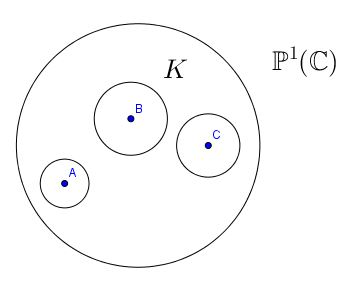
\includegraphics[width=5.7cm]{lezione-161024-fig1}
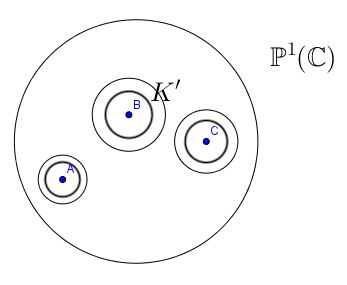
\includegraphics[width=6cm]{lezione-161024-fig2}
\caption{$K$ e $K'$}\label{fig:1}
\end{figure}

Quindi se $A, B, C$ sono i punti che si tolgono da $\mathbb{P}^1(\mathbb{C})$, allora si può scegliere $K'$ come $\mathbb{P}^1(\mathbb{C})\minus\{D_A\cup D_B\cup D_C\}$, con $D_A$ disco aperto attorno a $A$, $D_B$ disco aperto attorno a $B$, $D_C$ disco aperto attorno a $C$, perciò la proprietà.\\
Si osserva che la proprietà $\mathcal{P}$ è invariante per omeomorfismi quindi in particolare per biolomorfismi e che quindi non essendo soddisfatta dalle superfici di Riemann Sferica e Euclidee ne segue che $S$ è iperbolica.
Infatti si ha che si escludono le superfici compatte prendendo come $K'$ loro stesse, si esclude $\bbC$ prendendo come $K'$ il complementare di un disco aperto che contiene $K$ e si esclude $C^*=\mathbb{P}^1(\mathbb{C})\minus\{ 0,\infty\}$ perché con il ragionamento fatto per dimostrare la proprietà $\mathcal{P}$ su $S$ si dimostra che si trovano dei compatti $K'$ con $2$ componenti connesse, quindi non $almeno\hquad 3$, come richiesto dalla proprietà.
\end{itemize}
\end{proof}

\notamargine{La proprietà $\mathcal{P}$ in un qualche senso "conta i punti tolti, in funzione di quello che è rimasto". Inoltre permette di dire per esempio che un "toro meno $n$ punti distinti" non è omeomorfo a un "toro meno $m$ punti distinti", se $m\ne n$}

\begin{teorema}[Teorema di Picard]
Ogni funzione intera ($\bbC\rightarrow\bbC$ olomorfa su tutto $\bbC$) non costante assume tutti i valori tranne al più uno.
\end{teorema}

\begin{osservazione}
\begin{itemize}
\item La mappa esponenziale assume tutti i valori tranne lo $0$
\item Se la mappa $f$ come da ipotesi ha in più la proprietà di NON avere una discontinuità essenziale all'infinito allora si ha che per Liouville deve essere un polinomio, quindi il risultato è banale ($p(x)-a$ ha sempre almeno una radice, se $p$ non costante)
\end{itemize}
\end{osservazione}

\notamargine{C'è anche una versione più forte di questo teorema (detto da lui)}

\begin{proof}
Si usa che $\mathbb{P}^1(\mathbb{C})\minus\{ A, B, C\}$ con $A, B, C$ tre punti distinti è una superficie di Riemann iperbolica (Esercizio 7).\\
Si suppone per assurdo che $f$ soddisfacente le ipotesi non assuma due valori, che a meno di comporre $f$ con un'affinità (automorfismo di $\bbC$) suppongo essere $0,1$.
Allora $f$ induce una mappa olomorfa $f:\bbC->S$ (con $S$ come in Esercizio 7).
Si ha che quindi $f$ si solleva a $\tilde{f}:\bbC\rightarrow D$, con $D$ il disco aperto. DIAGRAMMA \\
Ma allora la mappa olomorfa $\tilde{f}$ è costante per Liouville, quindi poiché il diagramma commuta anche $f$ è costante, assurdo.
\end{proof}

\begin{osservazione}
\begin{itemize}
\item Questo è un teorema non di facile dimostrazione, il punto più delicato nella dimostrazione data è il teorema di Riemann.
\item Nella dimostrazione data il teorema di Riemann serve per l'esistenza di un rivestimento $\pi:D\cong \mathcal{H} \rightarrow S$. In effetti si può dimostrare il teorema di Picard esibendo un rivestimento, Picard face proprio così. Trovò il rivestimento quozientando $\mathcal{H}$ per il gruppo $\Gamma(2)=\{ \frac{az+b}{cz+d} | a,b,c,d\in \bbZ, ad-bc=1, a\cong d \cong 1 \pmod{2}, b\cong c \cong 0 \pmod{2} \}$, dopo aver dimostrato che questo gruppo agiste su $\mathcal{H}$ con le proprietà viste nelle scorse lezioni poiché effettivamente il quoziente sia una superficie di Riemann ed aver verificato che il quoziente è $S$.
\item Ci sono molte altre dimostrazioni con tecniche più analitiche, quella che si è fatta è più geometrica, senza stime. 
\end{itemize}
\end{osservazione}

\section{Biolomorfismi di tori}
D'ora in poi non ci si interessa più di superfici di Riemann iperboliche ma si iniziano a studiare i Tori, ovvero quozienti $\quotient{\bbC}{L}$ con $L$ reticolo di rango $2$.

\notamargine{Attenzione, molti matematici usano nella definizione di reticolo il fatto che il reticolo abbia la stessa dimensione dello spazio vettoriale in cui è contenuto, nel nostro caso è contenuto in $\bbC$ che ha dimensione reale $2$.}

\begin{osservazione}
Se prendiamo reticoli omotetici, ovvero due reticoli $L$ e $\lambda L$, con $\lambda \in \bbC\minus\{ 0\}$, si ha che i tori ottenuti sono biolomorfi. (La mappa moltiplicazione per $\lambda \quad \bbC \rightarrow \quotient{\bbC}{\lambda L} \hquad z\ \mapsto [\lambda z]_{\lambda L} $ è ben definita e passa al quoziente $\quotient{\bbC}{L}\rightarrow \quotient{\bbC}{\lambda L}$, che è olomorfa e ha come inversa olomorfa la moltiplicazione per $\lambda^{(-1)}$).
\end{osservazione}

\begin{fatto}Sia $f:T_1\rightarrow T_2$ olomorfa tra tori, con $T_i=\quotient{\bbC}{L_i},\hquad i\in \{ 1,2\}$, allora $\exists\alpha \hquad \alpha L_1\subseteq L_2$.\\
(CON ALPHA UGUALE A $0$ FUNZIONA SEMPRE, PROBABILMENTE INTENDE CHE SE $f$ NON NULLA ALLORA $\exists \alpha \ne 0 \hquad \alpha L_1\subseteq L_2$)
\end{fatto}
\begin{proof} Siano $\pi_i,\hquad i\in \{ 1,2\}$ le mappe di proiezione. DIAGRAMMA.
Si ha che la mappa $f\circ\pi_1: \bbC\rightarrow T_2$, siccome $\bbC$ è semplicemente connesso, si solleva a $\tilde{f}$ olomorfa (non necessariamente unica).
Prendendo $x_1\in T_1$, $z$ t.c. $\pi_1(z)=x$, allora $\pi_2\circ\tilde{f} (z) = f\circ \pi_1 (z)= f(x)$, quindi $\pi_2\circ \tilde{f}$ non dipende dal rappresentante $z$, ovvero $\pi_2\circ \tilde{f} (z+\lambda_1)=\pi_2\circ \tilde{f} (z)\hquad \forall \lambda_1\in L_1$.
Ma allora $\tilde{f} (z+\lambda_1) - \tilde{f} (z) \in L_2 \hquad \forall \lambda_1 \in L_1$.
Ma essendo $L_2$ discreto e $\tilde{f}$ continua si ha che $\tilde{f}(z+\lambda_1)=\tilde{f}(z)+c(\lambda_1)\hquad \forall z\in\bbC$, con $c(\lambda_1)\in L_2$ costante dipendente solo da $\lambda_1$.
Derivando l'ultima uguaglianza, si ha che $\tilde{f}'(z+\lambda_1)=\tilde{f}'(z) \hquad\forall \lambda_1\in L_1$.
Perciò la funzione $\tilde{f}'$ si quozienta ad una funzione  $T_1\rightarrow \bbC$ ne segue che la sua immagine è un compatto, quindi limitato e quindi per Liouville è costante. 
Perciò $\tilde{f}$ è lineare, $\tilde{f}(z)=\alpha z+\beta$.
Sostituendo questo in $\tilde{f} (z+\lambda_1) - \tilde{f} (z) \in L_2 \hquad \forall \lambda_1 \in T_1$ si trova $\alpha L_1\subseteq L_2$.
\end{proof}

\notamargine{Vedi anche Elliptic Function, Lang, pagina 14}

\begin{osservazione}
Non è detto che la mappa $f$ sia biunivoca come mappa $T_1\rightarrow T_2$, anche se la mappa "sopra" $\tilde{f}$ lo è.
\end{osservazione}

Viceversa se si ha $\alpha$ che soddisfa $\alpha L_1 \subseteq L_2$  allora la mappa moltiplicazione per $\alpha: \quad \bbC \rightarrow \quotient{\bbC}{L_2} \hquad z\ \mapsto [\alpha z]_{L_2} $ è ben definita e passa al quoziente $\quotient{\bbC}{L_1}\rightarrow \quotient{\bbC}{L_2}$.

\begin{osservazione}
\begin{itemize}
\item Tolta la traslazione $\beta$ (è un automorfismo di $\bbC$) le mappe indotte sui tori sono omomorfismi di gruppi.
\item A livello algebrico i tori hanno una realizzazione come gruppi con legge di gruppo razionale.
La mappa che manda tori in curve algebriche sono funzioni trascendenti (esempio esponenziale). MAH
\end{itemize}
\end{osservazione}


\begin{fatto} Considero $f$ omomorfismo di gruppi e biolomorfismo, quindi indotta da $\tilde{f}=\alpha z$. Allora $\alpha L_1=L_2$.
\end{fatto}
\begin{proof}
Sia $[z]_{L_1} \mapsto [\alpha z]_{L_2}$ indotta dalla moltiplicazione per $\alpha$, se è invertibile considero gli elementi $[\frac{\lambda_2}{\alpha}]_{L_1}, \lambda_2 \in L_2$, allora questi vengono mandati in $0$ dalla mappa $f$, poiché è iniettiva, ovvero tutti i $\frac{\lambda_2}{\alpha}$ devono stare in $L_1$, ovvero $\frac{1}{\alpha} L_2 \subseteq L_1 \Rightarrow L_2 \subseteq \alpha L_1$.
Quindi siccome sapevo già che $\alpha L_1 \subseteq L_2$ ho trovato che $\alpha L_1 =L_2$.
\end{proof}

\begin{esercizio} Sia $f$ omomorfismo olomorfo tra tori, allora il nucleo è un insieme finito, ed è misurato da $\quotient{L_2}{\alpha L_1}$ (quoziente di due gruppi, uno sottogruppo di quell'altro).
\end{esercizio}

\begin{esercizio}
L'indice di un reticolo di rango $2$ contenuto in un altro è finito.
\end{esercizio}

\notamargine{Suggerimento: prendere gli elementi di base.\\ Esempio: $n\bbZ \oplus m\bbZ \le \bbZ \oplus \bbZ$ ha indice $nm$.}

\begin{osservazione}
\begin{itemize}
\item Si è dimostrato che due tori sono biolomorfi se e solo se i reticoli sono omotetici, in formule $T_1\cong T_2 \iff \exists \alpha\in\bbC^* \alpha L_1=L_2$.
\item Nota che due Tori sono sempre isomorfi come spazi topologici, come varietà reali e come gruppi di Lie (gruppi analitici reali).
\item Che siano omeomorfi come superfici di Riemann, ovvero che i reticoli soddisfino $\exists \alpha\in\bbC^* \alpha L_1=L_2$  è una condizione molto forte 
\end{itemize}
\end{osservazione}


\section{Spazio dei parametri}
Si ha che la condizione sui reticoli ci permette di analizzare lo spazio di parametri per i tori.

Preso un reticolo generico $L=\omega_1 \bbZ + \omega_2 \bbZ$ con $\Im \frac{\omega_1}{\omega_2} \ne 0$ si ha che, se si sceglie l'orientazione con $\Im \frac{\omega_1}{\omega_2}>0$ (a meno di scambiare $\omega_1$ con $\omega_2$), il toro è omotetico a $\frac{1}{\omega_2} L= \tau \bbZ+ \bbZ$, con $\tau=\frac{\omega_1}{\omega_2} \in \mathcal{H}$. 

La base in $\{\omega_1, \omega_2 \}$ non è determinata, infatti posso fare qualsiasi cambio di base con matrice $	\begin{pmatrix} a & b \\ c & d \end{pmatrix}$ con $a,b,c,d \in \bbZ$ e $ad-bc=\pm 1$. (invertibile)

Se però considero le basi orientate, ovvero se dalla base $\{\omega_1, \omega_2 \}$ con $\Im \frac{\omega_1}{\omega_2}>0$ passo alla base $\{\omega_1', \omega_2' \}$ con $\Im \frac{\omega_1'}{\omega_2'}>0$, allora si ha che $\tau'=\frac{\omega_1'}{\omega_2'}=\frac{a\tau +b}{c\tau+d}=\frac{ac |\tau |^2+bd+ad\tau +bc \bar\tau}{|c\tau+d|^2}$, quindi $\Im\tau'=\frac{(ad-bc)}{ |c\tau+d|^2} \Im(\tau-\bar\tau)$ ma siccome $\Im(\tau-\bar\tau)=\frac{(\tau-\bar\tau)-\overline{(\tau-\bar\tau)}}{2i}=\frac{2\tau-2\bar\tau}{2i}=2(\Im\tau)$ allora $\Im\tau'$ ha lo stesso segno del determinante.

Cioè abbiamo visto che le matrici di cambio di base, se conserviamo l'orientazione, sono le matrici di $SL_2(\bbZ)$, ne risulta che lo spazio dei tori complessi di dimensione complessa $1$ a meno di biolomorfismo è $\quotient{\mathcal{H}}{SL_2(\bbZ)}$.

\begin{osservazione}
\begin{itemize}
\item Non è ovvio vedere cosa sia quel quoziente.
\item Topologicamente è $\bbC$.
\item $SL_2(\bbZ)$ ha dei punti fissi, quindi il quoziente non è una superficie di Riemann con la mappa indotta da $\mathcal{H}$.
\item per avere superfici di Riemann devo prendere gruppi che soddisfano le famose proprietà, per esempio $\Gamma (2)$.
\item Le matrici di quel tipo sono numerabili, $\mathcal H$ ha la cardinalità del continuo, quindi il quoziente ha la cardinalità del continuo.
\item Un dominio fondamentale (contiene un punto per ogni classe di biolomorfismo di tori) è dato da $\{ x+iy | -\frac{1}{2}<x<\frac{1}{2}, y>\sqrt{1-x^2}\}$. (Figura 1)
Si noti che torna che la cardinalità sia quella del continuo, anche senza aver visto che è un quoziente. (Dimostrazione di queste cose???)
\end{itemize}
\end{osservazione}

\begin{figure}[h]
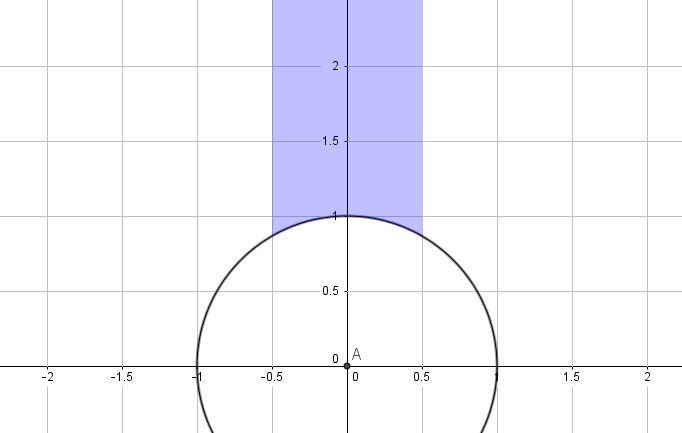
\includegraphics[width=8cm]{lezione-161024-fig3}
\caption{Dominio fondamentale}\label{fig:2}
\end{figure}

Anticipazione: la prossima volta si vedranno gli automorfismo di un reticolo e i gruppi olomorfi, per questi ultimi si darà un cenno al concetto di funzione olomorfa in più variabili.

\chapter{26/10/2016 - Delle Cose}
	Abbiamo distinto le superfici di Riemann in tre tipi:
	\begin{itemize}
	 \item La superficie sferica $\hat\bbC$;
	 \item Le superfici euclidee, ottenute quozientando $\bbC$;
	 \item Le superfici iperboliche, ottenute da quozienti del disco $D$.
	\end{itemize}

	\begin{proposizione}
		Ogni mappa biolomorfa da una superficie sferica a una euclidea è costante. Allo stesso modo, ogni mappa biolomorfa da una superficie euclidea a una iperbolica è costante.
	\end{proposizione}
	
	\begin{proof}
		Siano $S_1$, $S_2$ e $S_3$ tre superfici, rispettivamente sferica, euclidea e iperbolica, e siano $f: S_1 \rar S_2$, $g: S_2 \rar S_3$ mappe biolomorfe, come nel diagramma.
		
		% INSERIRE DIAGRAMMA
		
		Poichè sia $\hat\bbC$ sia $\bbC$ sono semplicemente connessi, per il solito lemma $f \circ \pi_1$ e $g \circ \pi_2$ si sollevano a $\tilde f, \tilde g$. 
		
		Ma $\tilde f$, ristretta a $\bbC$, è una mappa intera (olomorfa su $\bbC$) limitata (perchè all'infinito deve tendere ad $f(\infty)$). Quindi per Liouville è costante.
		Stesso discorso vale per $\tilde g$, che è olomorfa su $\bbC$ ed è limitata (ha immagine contenuta nel disco). Quindi anche $f$ e $g$ devono essere costanti.
		
		
	\end{proof}
	
	Restringiamoci ora ai tori. Una mappa tra due tori $T_1 = \bbC/L_1$ e $T_2 = \bbC/L_2$ abbiamo visto che deve essere della forma $f(z)=\alpha z + \beta$.\notamargine{D'ora in poi faremo spesso confusione tra un numero complesso e la sua classe di equivalenza.}
	
	\begin{definizione}
		Una legge di gruppo olomorfa su una superficie di Riemann $S$ è una legge di gruppo in cui la moltiplicazione e l'inverso sono mappe biolomorfe rispettivamente da $S \times S$ a $S$ e da $S$ a $S$ (per un'opportuna definizione di mappa biolomorfa da una varietà bidimensionale).
	\end{definizione}
	
	Su un toro abbiamo un'ovvia legge di gruppo ereditata dalla somma su $\bbC$. Inoltre possiamo mettere una legge di gruppo isomorfa, in cui cambio l'origine. Questo si può fare in generale: data la moltiplicazione $\cdot$ su un gruppo $G$, posso definire l'operazione $g * h = g\cdot a^{-1}\cdot h$, con $a\in G$. Allora $(G,*)$ ha $a$ come origine, e ho l'ovvio isomorfismo tra $(G,\cdot)$ e $(G,*)$ dato da $g\mapsto g\cdot a$.
	
	\begin{proposizione}
		A meno di cambi di origine, ho una sola legge di gruppo olomorfa sul toro $T$.
	\end{proposizione}
	
	\begin{proof}
		Sia $x \in T$, sia $*$ una legge di gruppo e sia senza perdita di generalità $0$ l'elemento neutro. Consideriamo la funzione $\phi_x: z \mapsto x * z - x$.

		Questa è una mappa biolomorfa tra tori, e sappiamo che deve essere della forma $z \mapsto \alpha z + \beta$. Ma $\phi_x(0)=0$, quindi $\beta=0$. Sia quindi $c_x \in \bbC$ tale che $\phi_x(z)=c_xz$.
		
		Quindi abbiamo, riarrangiando i termini della definizione 
		\[
		 x*z = \phi_x(z) + x = c_xz + x
		\]
		(ricordiamo che si tratta di numeri complessi modulo il reticolo $L$).
		
		Fissiamo ora $z_0\ne 0$. $c_x$ è una funzione olomorfa in $x$, infatti, detta $f(\zeta) = \zeta * z_0$, vale
		\[
			f(\zeta) = \zeta + c_\zeta z_0 + \lambda, \lambda \in L
		\]
		stavolta pensata su $\bbC$. Quindi posso ricavare $c_\zeta$, e dato che $f$ è olomorfa per ipotesi, ottengo quello che volevo.
		
		D'altra parte, fissato un qualsiasi $\lambda \in L$, allora $c_x\lambda \in L \; \forall x$, quindi poichè $x \mapsto c_x \lambda$ è olomorfa a valori in un discreto, deve essere localmente costante e quindi costante. Sia quindi $c=c_x$.
		
		Ponendo $x=0$ ottengo che $\phi_0(z) = cz = z$, da cui $c=1$.


	\end{proof}

	% Aggiungere delirio su Aut(D)
	
	\section{Tori}
	
	Torniamo ora sull'argomento principale del corso, che sono i tori. Sia $T = \bbC / L$ un toro, con $L$ reticolo, con la struttura di gruppo indotta da $\bbC$.
	
	Siano ora $\Aut_0(T)$ gli automorfismi che fissano l'origine. Abbiamo visto che sono solo le omotetie di fattore $\mu$ che fissano il reticolo. sicuramente nel reticolo ho un complesso di norma minima, essendo un insieme discreto: ma allora la norma minima deve conservarsi dopo l'omotetia, quindi $\abs \mu=1$.
	
	Inoltre, dato un qualsiasi $\lambda_0 \in L$, vale $\abs{\lambda_0 \mu} = \abs \lambda_0$, da cui segue che $\Aut_0(T)$ è finito; essendo un sottogruppo di $\bbC^*$, per un noto lemma è anche ciclico.
	
	Fissando una base del reticolo, ogni automorfismo si scrive come una matrice $2 \times 2$ a coefficienti interi. Per qualche strano motivo da capire che c'entra con le radici dell'unità, %TODO%
	posso avere solo rotazioni di $180, 90, 60$.
	
	\subsection{Isogenie}
	
	\begin{definizione}
		Una mappa $c: T_1 \rar T_2$ si dice un'isogenia se è un'omomorfismo suriettivo (di gruppi olomorfi).

	\end{definizione}
	
	\begin{proposizione}
		$\Ker c$ è finito.
	\end{proposizione}
	\begin{proof}
		Da fare.
	\end{proof}
	
	\begin{definizione}
		Si dice grado dell'isogenia $[L_2 : \mu L_1]$.
	\end{definizione}
	
	\begin{osservazione}
		La composizione di due isogenie è un'isogenia che ha come grado il prodotto dei gradi.
	\end{osservazione}
	
	Attenzione! Il fattore $\mu$ non dipende solo dal toro, ma anche dal fattore di omotetia. In altre parole, quando quoziento penso il toro come un elemento del quoziente $\{ \mbox{reticoli} \} / \{ \mbox{omotetia} \}$, $\mu$ non è indipendente dal rappresentante, ma dipende dal reticolo scelto.
	
	\begin{osservazione} 
		Gli isomorfismi sono un sottoinsieme proprio delle isogenie.
	\end{osservazione}




	
	


	
	


%% Lezione di esempio. Copiate questo file nella lezione che dovete creare
%% per avere già uno scheletro di come scrivere le lezioni

%% Diamo un nome al capitolo. Idealmente mettiamo la data della lezione ed
%% una sua breve descrizione / argomenti trattati
\chapter{02/11/16 - Isogenie dei Tori e Anello degli Endomorfismi}
\justify

%% Le parole dentro a \newthought vengono scritte in maiuscoletto. Usatele
%% per sottolineare meglio alcune parole ad inizio paragrafo
\newthought{Avevamo}  mostrato, nelle lezioni precedenti, che il $ \bbP_{1}\bbC $ non ammette strutture di gruppo olomorfo. \\
Abbiamo inoltre mostrato che i tori ammettono come unica struttura di gruppo quella di gruppo quoziente di $\bbC$ sul reticolo $L$.\\


%% Si può poi inserire una section per scrivere degli argomenti specifici
\section{Leggi di gruppo su superfici di Riemann}
\begin{osservazione}
Sia G un gruppo olomorfo. $\forall g \in G$ le traslazioni $L_{g}$ e $R_{g}$ sono mappe biolomorfe senza punti fissi. 
\end{osservazione}

\noindent Il nostro obiettivo, in questa sezione, è quello di mostrare come nessuna superficie di Riemann iperbolica ammetta una struttura di gruppo olomorfo. In realtà ci basterà mostrarlo solo per il disco unitario grazie al seguente lemma:
\begin{lemma}
Sia $X$ un gruppo topologico con $\mu : X\times X \rar X$ legge di gruppo. Sia inoltre $p :\widetilde{X} \rar X$ il rivestimento universale.
Allora $\mu$ si solleva ad una $\tilde{\mu} : \widetilde{X} \times \widetilde{X} \rar \widetilde{X}$ che rende $\widetilde{X}$ un gruppo topologico.
\end{lemma}

\begin{proof}

			\begin{diagram}
				\widetilde{X}\times\widetilde{X}	& \rTo^{\widetilde{\mu}} 	& \widetilde{X}	\\
				\dTo<{p \times p}	&					& \dTo>{p}\\
				X\times X				& \rTo^\mu 		& X 
			\end{diagram}

\noindent Sia $e \in X$ l'identità di $X$ e sia $\tilde{e} \in \widetilde{X}$ un punto t.c. $p(\tilde{e})=e$. Prodotto di semplicemente connessi è semplicemente connesso, dunque la mappa $\mu \circ (p \times p)$ solleva ad una mappa $\widetilde{\mu}$ che chiude il diagramma. Basta ora mostrare che $\widetilde{\mu}$ è una legge di moltiplicazione {\it (un po' di verifiche emozionantissime)}.\\

{\bf Elemento neutro:}
	\begin{diagram}
		\{\tilde{e}\}\times\widetilde{X}	& \rTo^{\widetilde{\mu}}_{\pi_{2}} 	& \widetilde{X}	\\
		\dTo<{p \times p}			&					& \dTo>{p}\\
		\{e\}\times X				& \rTo^\mu 				& X 
	\end{diagram}

\noindent Per restrizione, $\tilde{\mu}$ chiude il diagramma. Ma anche la proiezione sul secondo fattore fa commutare il quadrato; per unicità del sollevamento a punto base fissato si ha che $\tilde{\mu}(\tilde{e}, \bullet) \equiv \pi_{2}(\bullet)$. Analogamente si ha che $\tilde{\mu}(\bullet, \tilde{e}) \equiv \pi_{1}(\bullet)$ e dunque $\tilde{e}$ è elemento neutro per $\tilde{\mu}$.\\
{\bf Associatività} e {\bf inverso} si ottengono in maniera del tutto analoga (cioè sfruttando l'unicità del sollevamento).
\end{proof}

\begin{teorema}
Il disco unitario in $\bbC$ non ammette una struttura di gruppo olomorfa
\end{teorema}

\begin{proof}
Per assurdo; ci sono due possibili vie.\\
Conoscendo i gruppi di Lie, basta considerare la mappa esponenziale dal tangente nel disco: dovrebbe essere una mappa non costante da $\bbC$ nel disco. \hfill \Lightning \\
Altrimenti, sia $\star : D\times D \rar D$ una legge di gruppo olomorfa. Sia inoltre $x^{*}$ l'inverso di $x$ per $\star$. Senza perdita di generalità, si può supporre che $0 \in D$ sia l'elemento neutro.
Allora $\forall x\in D$ la mappa $L_{x}: z\mapsto x\star z$ è un automorfismo olomorfo. \\
Dunque,  $$x\star z = c(x)\frac{z -a(x)}{1- \overline{a}(x) z}$$
con $|c(x)|\equiv 1$ e $a:D \rar D$.\\
Per $z=0$ si ha $x=-c(x)a(x)$.\\
Per $z=a(x)$ si ha $x*a(x)=0$ $\Rar$ $a(x)=x^{*}$ $\Rar$ $a(x)$ è olomorfa $\Rar$ (per $x\neq 0$) $c(x)=-\frac{x}{x^{*}}$ $\Rar$ $c(x)$ è olomorfa per $x\neq 0$, ma $|c(x)| \equiv 1$ $\Rar$ per il teorema della mappa aperta deve essere $ \ c(x) \equiv k \neq 0$. Da cui $a(x)= -\frac{x}{k}$.\\
Allora, $$x\star 1/2 = k\frac{1-2a(x)}{2-\overline{a}(x)}$$
ma questa non è olomorfa ( $\overline{a}(x)$ non lo è, il resto sì). 

\end{proof}

\begin{corollario}
Curve algebriche non ellittiche \underline{non} ammettono struttura di gruppo olomorfo.
\end{corollario}
%% Le subsection sono, ovviamente, le sottosezioni. State attenti però che
%% con il tipo di testo che stiamo usando le subsubsection non esistono

\section{Endomorfismi di un Toro}

\newthought{In questa sezione} vogliamo studiare l'anello delle isogenie di un toro in sè. Ma prima classifichiamo un po' meglio le isogenie tra tori.

\begin{proposizione}
Siano $T_{1}$ e $T_{2}$ due tori.\\
$\exists f:T_{1} \rar T_{2}$ isogenia $\sse$ $\exists \Gamma < T_{1}$ sottogruppo finito t.c. $\sfrac{T_{1}}{\Gamma} \simeq T_{2}$ come gruppi olomorfi. 
\end{proposizione}
\begin{proof}
\fbox{$\Rar$}\\
\'E il primo teorema di omomorfismo (ci sarebbe da mostrare che gli isomorfismi sono olomorfi ma ci crediamo).\\
\fbox{$\Leftarrow$}\\
Sia $\pi:\bbC \rar T_{1} = \sfrac{\bbC}{L}$ la proiezione al quoziente. Allora $\overline{L}=\pi^{-1}(\Gamma)$ è un sottogruppo discreto di $\bbC$ (rimane discreto perche $\Gamma$ è finito). Per teoremi di omomorfismo (di nuovo sarebbe da mostrare l'olomorfia):
$$\sfrac{T_{1}}{\Gamma} \simeq \sfrac{\sfrac{\bbC}{L}}{\Gamma} \simeq \sfrac{\bbC}{\overline{L}}$$
Di conseguenza $\sfrac{T_{1}}{\Gamma}$ è un toro $T_{2}$ e la proiezione al quoziente è isogenia tra $T_{1}$ e $T_{2}$.
\end{proof}

Più avanti definiremo le funzioni di Weierstrass, che ci permetteranno di trasformare i tori in curve algebriche (ellittiche). Le isogenie verranno trasformate in funzioni razionali tra le curve.

\subsection{Anello degli Endomorfismi di un Toro}

Fissiamo un toro $T=\sfrac{\bbC}{L}$ e consideriamo l'insieme $End(T)$ delle isogenie del toro in sè, con in più la mappa nulla.

\begin{proposizione} $End(T)$ ha una naturale struttura di anello (somma tra mappe e prodotto di composizione). Inoltre vale che:
\begin{enumerate}
\item $End(T)$ è un anello commutativo
\item $\bbZ \subseteq End(T)$
\item $End(T) \hookrightarrow \bbC$
\item $End(T) \otimes_{\bbZ} \bbQ$ è un campo ({\it d'ora in poi, se non diversamente specificato, tutti i tensori saranno su $\bbZ$})
\end{enumerate}
\end{proposizione}

\begin{proof} {\it Lui ha dato tutto ciò per buono. Non so quanto sia utile dimostrarlo ma vabbè}\\
3.\\
Abbimo mostrato precedentemente che ogni isogenia è passaggio al quoziente di un'opportuna moltiplicazione per scalare su $\bbC$. Per gli endomorfismi vale un risultato più forte: lo scalare che induce l'isogenia è unico.
Infatti, siano $\lambda$ e $\mu$ elementi di $\bbC$ che inducono la stessa isogenia $f:T\rar T$. Allora, $\forall x\in \bbC,  \ (\lambda - \mu)x \in L$. Quindi, l'ideale generato da $\lambda -\mu$ deve essere contenuto nel reticolo, che è discreto $\Rar$ $\lambda - \mu = 0$. \'E quindi ben definita la mappa $f \mapsto \mu$ che associa ad ogni endomorfismo lo scalare di cui è passaggio al quoziente. Questa mappa è chiaramente un omomorfismo iniettivo di anelli.\\
1.\\
ovvia dalla 3.\\
2.\\
Poichè $L$ è uno $\bbZ$-modulo, $\forall n \in \bbZ, nL\subseteq L$. Inoltre, sia $x\in \bbC \setminus L$. Allora $x/n \not\in L$ e si ha che $n[x/n]=[x]$ $\Rar$ la moltipicazione per n è surgettiva sul toro $\Rar$ $\bbZ \subseteq End(T)$\\
4.\\
Sia $t=\sum\limits_{i=0}^{k} \mu_{i} \otimes \frac{p_{i}}{q_{i}}$. Sia $q$ il minimo comune multiplo dei $q_{i}$ e siano $a_{i} \in \bbZ$ tali che $\forall i, q=q_{i}a_{i}$. Allora,\\
$t=\sum\limits_{i=0}^{k} \mu_{i}\otimes \frac{p_{i}}{q_{i}} = \sum\limits_{i=0}^{k} \mu_{i} \otimes \frac{p_{i}a_{i}}{q}= \sum\limits_{i=0}^{k} a_{i}p_{i}\mu_{i}\otimes \frac{1}{q} = (\sum\limits_{i=0}^{k} a_{i}p_{i}\mu_{i})\otimes \frac{1}{q}$ $\Rar$ ogni tensore è semplice. L'inverso di un tensore $\mu \otimes \frac{p}{q}$ (dove $\mu$ è una mappa non nulla di grado $d$) è il tensore $\hat{\mu} \otimes \frac{q}{pd}$, con $\hat{\mu}$ l'endomorfismo duale di $\mu$ (la moltiplicazione è quella indotta sull'anello tensore dai due anelli $End(T)$ e $\bbQ$. Sui tensori semplici diventa semplicemente la moltiplicazione "componente per componente").
\end{proof}

Volendo, potremmo fare gli stessi discorsi (anello degli endomorfismi etc...) sulle curve ellittiche (che sono definite anche su altri campi). Cosa cambia? In $char \ K >0$ {\bf non } è detto che $End(T)$ sia commutativo (con $T$ curva ellittica).\\

\noindent Cerchiamo ora di caratterizzare un po' meglio $F=End(T) \otimes \bbQ$. Sia $T=\tau \bbZ + \bbZ$ e $\mu : T \rar T$ l'isogenia indotta dalla moltiplicazione per $\mu$. La condizione di mappare il reticolo in sé si traduce nel sistema:
\begin{equation*}
\begin{cases}
	\mu \tau = a\tau + b\\
	\mu = c\tau + d\\
\end{cases}
\end{equation*}
Con $M=
\begin{pmatrix}
a & b \\
c & d
\end{pmatrix}$, $ \ M\in \mathfrak{M}_{2}(\bbZ)$.\\
Se $\bar{\mu}=\mu$ $\Rar$ $c=0$ $\Rar$ $\mu \in \bbZ$.\\
Altrimenti $\mu$ è quadratico immaginario perchè è autovalore della matrice $M$, ma non razionale.
Quando posso avere i due casi?\\
Si deve avere $\tau = \frac{a\tau + b}{c\tau + d}$ $\Rar$ $c\tau^{2} + (d-a)\tau - b=0$\\
$\tau$ non è immaginario quadratico $\Rar$ $End(T)=\bbZ$.
$\tau$ è immaginario quadratico $\Rar$ $\bbZ \subsetneq End(T)$. Questo fenomeno si chiama {\bf moltiplicazione complessa dei tori}.

\newthought{Chi è} il rappresentante del duale di una isogenia?\\
La moltiplcazione tra i due rappresentanti deve dare il grado dell'isogenia $\Rar$ $\hat{\mu} = \overline{\mu}$. 
\begin{corollario}
$\hat{\mu + \nu} =\hat{\mu} + \hat{\nu}$
\end{corollario}

\noindent {\bf $\underline{\mbox{Esercizio:}}$} $c_{i}: T_{1} \rar T_{2}$ ($i=1 , 2$) isogenie, $c_{1}+c_{2} \neq 0$ $\Rar$ $\hat{c_{1} + c_{2}}=\hat{c_{1}}+\hat{c_{2}}$.\\
{\bf $\underline{\mbox{Hint:}}$} $\hat{c_{2}}\circ c_{1} \in End(T_{1})$


\newcommand{\res}{\text{res}}
\newcommand{\ord}{\text{ord}}
\newcommand{\im}{\text{im}}

\chapter{07/11/16}
\justify


Prendiamo $T_1=\bbC/L_1$ e $T_2=\bbC/L_2$ tori complessi.
Ogni morfismo (omomorfismo di gruppi che sia anche olomorfo) $T_1\rar T_2$ si solleva ad un unico morfismo $\bbC\rar\bbC$, che è per forza dato dalla moltiplicazione per una costante.
Se rappresentiamo $T_1$ e $T_2$ come quozienti di $\bbC$ in un modo diverso, la costante può cambiare (quindi non è canonica).
Tuttavia, se $T_1=T_2$ allora la costante è determinata in modo canonico (quella ottenuta rappresentando $T_1$ e $T_2$ nello stesso modo come quozienti di $\bbC)$.


\begin{teorema}\label{puppa}
$T$ un toro e $f:T\rar\bbC$ meromorfa (non costante). Allora

(i) $\sum_{x\in T}\res_xf=0$ $\qquad$ (uguaglianza di numeri complessi)

(ii) $\sum_{x\in T}\ord_xf=0$ $\qquad$ (uguaglianza di numeri interi)

(iii) $\sum_{x\in T}x\cdot\ord_xf=0$ $\qquad$ (uguaglianza di elementi del gruppo $T$)
\end{teorema}

\notamargine{$\res_xf$ indica il residuo di $f$ in $x$ (e $0$ se $f(x)\in\bbC$)}

\notamargine{$\ord_xf$ indica la molteplicità di $x$ come radice di $f(x)=0$, o l'opposto dell'ordine del polo in $x$ (e $0$ se $f(x)\in\bbC\setminus\{0\}$)}

\begin{proof}
$f^{-1}(0)$ è finita: se fosse infinita, allora dovrebbe accumularsi da qualche parte su $T$ (per compattezza), e quindi $f$ sarebbe costante (per prolungamento analitico).
Analogamente l'insieme dei punti in cui $f$ non è definita è finito.

Scegliamo una rappresentazione $T=\bbC/L$ con $L=\{a\omega_1+b\omega_2 : a,b\in\bbZ\}$. Prendiamo la funzione biperiodica $F:\bbC\rar\bbP^1$ data da $\bbC\rar T\xrightarrow{f}\bbP_1$.

Sia $\gamma:[0,1]\rar\bbC$ un cammino che percorre il bordo di un parallelogrammo del reticolo (un solo giro, verso antiorario):
possiamo supporre che in $\im\gamma$ valga $F\in\bbC\setminus\{0\}$ (a meno di traslare $\gamma$).

(i) Uso il teorema dei residui sulla funzione $F$ con il gammino $\gamma$: ottengo

$2\pi i\sum_{x\in T}\res_xf=\int_\gamma F=(\int_0^{\omega_1}F-\int_{\omega_2}^{\omega_1+\omega_2}F)+(\int_{\omega_1}^{\omega_1+\omega_2}F-\int_{0}^{\omega_2}F)$

ed entrambe le parentesi si annullano per biperiodicità di $F$.

\notamargine{Un po' di libertà di notazione}

(ii) Identico ad (i), usando la funzione $\frac{F'}{F}$ al posto di $F$ (osservo che $\frac{F'}{F}$ è ancora biperiodica) (osservo che $\res_x\frac{F'}{F}=\ord_xF$).

(iii) Uso il teorema dei residui sulla funzione $z\frac{F'(z)}{F(z)}$ con il cammino $\gamma$.

Notare che $\res_xz\frac{F'(z)}{F(z)}=x\cdot\res_x\frac{F'}{F}=x\cdot\ord_xF$.

Ottengo $2\pi i\sum_{x\in T}x\cdot\ord_xf=\int_\gamma z\frac{F'(z)}{F(z)}\ dz=(\int_0^{\omega_1}-\int_{\omega_2}^{\omega_1+\omega_2})+(\int_{\omega_1}^{\omega_1+\omega_2}-\int_{0}^{\omega_2})$

e per biperiodicità si ha $\int_{\omega_2}^{\omega_1+\omega_2}z\frac{F'z}{Fz}\ dz=\int_0^{\omega_1}(z-\omega_2)\frac{F'z}{Fz}\ dz$ quindi

$(\int_0^{\omega_1}-\int_{\omega_2}^{\omega_1+\omega_2})=\omega_2\int_0^{\omega_1}\frac{d}{dz}(\log F)\ dz=\omega_22\pi i m$ per qualche $m\in\bbZ$
(più precisamente, $m$ è il numero di giri che fa $\log F$ intorno a $0$ quando $z$ varia da $0$ a $\omega_1$).

Quindi $\sum_{x\in T}x\cdot\ord_xf$ è un elemento del reticolo $L$, da cui la tesi.
\end{proof}


Fissiamo un toro $T$ e rappresentiamolo come $\bbC/L$ ($L$ reticolo).
Consideriamo la serie di funzioni definite sull'aperto $\bbC\setminus L$ a valori in $\bbC$ data da $\frac{1}{z^2}+\sum_{\omega\in L\ \omega\not=0}(\frac{1}{(z-\omega)^2}-\frac{1}{\omega^2})$.

\begin{proposizione}
La serie sopra converge totalmente (e quindi uniformemente) sui compatti contenuti in $\bbC\setminus L$.
\end{proposizione}
\begin{proof}(sketch)

Fissiamo $K\subseteq\bbC\setminus L$ compatto.

Si ha $\sup_{z\in K}\abs{\frac{1}{(z-\omega)^2}-\frac{1}{\omega^2}}=\sup_{z\in K}\abs{\frac{z(2\omega-z)}{\omega^2(z-\omega)^2}}$ che per $\omega$ 'lontano' da $K$ è circa $\abs{\frac{1}{\omega^3}}$.

Ma $\sum_{\omega\in L\setminus\{0\}}\abs{\frac{1}{\omega^3}}$ converge, perchè
gli $\omega$ di modulo $R$ sono circa $R$, e quindi quella è circa $\sum R\cdot\frac{1}{R^3}=\sum\frac{1}{R^2}<+\infty$.
\end{proof}

Quindi il limite della serie sopra è una funzione olomorfa $P:\bbC\setminus L\rar\bbC$.

\'E inoltre facile (non del tutto ovvio, TO DO) verificare che $P$ è una funzione $L$-biperiodica.

Se prendiamo la serie che definisce $P$ e togliamo il termine $\frac{1}{z^2}$, converge uniformemente in un intorno di $0$ (e analogo per ogni $\omega\in L$).
Quindi $P$ è meromorfa su tutto $\bbC$.

Fattorizzando $P$, otteniamo una funzione meromorfa $\wp:T\rar\bbC$, chiamata \textbf{funzione di Weierstrass} (tale definizione dipende dal reticolo $L$ scelto per rappresentare $T$? TO DO).

\begin{proposizione}
La funzione meromorfa $\wp:T\rar\bbC$ ha le seguenti proprietà:

(i) $\wp(-z)=\wp(z)$.

(ii) $\wp$ ha un polo doppio in $0$ e nessun altro polo.

(iii) Fissato $u\in T$ con $u\not=-u$, si ha $\ord_u(\wp-\wp(u))=\ord_{-u}(\wp-\wp(u))=1$ e $\ord_0(\wp-\wp(u))=-2$ e $\ord_x(\wp-\wp(u))=0$ per $x\not=0,u,-u$.

In altre parole, $\wp-\wp(u)$ ha uno zero semplice in $u$, uno zero semplice in $-u$, un polo doppio in $0$ e nessun altro zero o polo.

(iii') Fissato $u\in T$ con $u=-u\not=0$, si ha $\ord_u(\wp-\wp(u))=2$ e $\ord_0(\wp-\wp(u))=-2$ e $\ord_x(\wp-\wp(u))=0$ per $x\not=0,u$.

In altre parole, $\wp-\wp(u)$ ha uno zero doppio in $u$, un polo doppio in $0$ e nessun altro zero o polo.
\end{proposizione}
\begin{proof}
(i) Ovvio direttamente dalla definizione (riordinando gli addendi).

(ii) Ovvio (perchè sappiamo dove stanno i poli di $P$).

(iii) Prendiamo la funzione meromorfa $\wp-\wp(u):T\rar\bbC$ e usiamo il teorema \ref{puppa} (grazie a (ii) sappiamo dove questa ha poli e con che molteplicità).

(iii') Idem come (iii).
\end{proof}


\begin{teorema}
Non esiste un polinomio $A\in\bbC[x]$ tale che $A(\wp):T\rar\bbC$ sia la funzione costantemente nulla.
\end{teorema}
\begin{proof}
Sia $A(x)=(x-a_1)...(x-a_n)$. Se $A(\wp)\equiv0$, allora almeno una tra le $(\wp-a_i)$ dovrebbe essere $\equiv0$, ma $\wp-a_i$ ha un polo doppio in $0$...
\end{proof}


\begin{teorema}
Il campo delle funzioni meromorfe pari $T\rar\bbC$ è $\bbC(\wp)$.
\end{teorema}
\begin{proof}
Prendiamo $f:T\rar\bbC$ meromorfa pari (non costante).

Prendiamo $u\not=-u$ con $\ord_uf\not=0$ (quindi uno zero o un polo). Allora $\ord_{-u}f=\ord_uf$ e possiamo considerare $f\cdot(\wp-\wp(u))^{-\ord_uf}$:
questa è meromorfa pari ed ha gli stessi zeri e poli di $f$ (con le stesse molteplicità) eccetto
in zero ed in $u,-u$ (in cui $\ord_uf\cdot(\wp-\wp(u))^{-\ord_uf}=\ord_{-u}f\cdot(\wp-\wp(u))^{-\ord_uf}=0$).
Sostituiamo $f$ con $f\cdot(\wp-\wp(u))^{-\ord_uf}$.

Prendiamo $u=-u\not=0$ con $\ord_uf\not=0$. Allora $\ord_uf$ è pari (se $u$ è uno zero, osserviamo che $f'$ è dispari e quindi $f'(u)=0$, e analogo per tutte le derivate di ordine dispari;
se $u$ è un polo, facciamo lo stesso ragionamento su $\frac{1}{f}$). Possiamo quindi considerare $f\cdot(\wp-\wp(u))^{-\frac{1}{2}\ord_uf}$:
questa è meromorfa pari ed ha gli stessi zeri e poli di $f$ (con le stesse molteplicità) eccetto in zero ed in $u$ (in cui $\ord_uf\cdot(\wp-\wp(u))^{-\frac{1}{2}\ord_uf}=0$).
Sostituiamo $f$ con $f\cdot(\wp-\wp(u))^{-\frac{1}{2}\ord_uf}$.

Reiterando le operazioni sopra descritte, otteniamo un'uguaglianza del tipo $f\cdot\frac{A(\wp)}{B(\wp)}=g$ con $g$ meromorfa pari senza zeri e poli eccetto eventualmente in $0$.
Ma dal teorema \ref{puppa} otteniamo che $g$ non ha uno zero o polo nemmeno in $0$. Ma allora $g$ deve essere costante
(sollevate $g:T\rar\bbC$ ad una $G:\bbC\rar\bbC$: vi viene che $G$ è olomorfa su tutto $\bbC$ e biperiodica, quindi limitata, e quindi costante per Liouville).

Quindi $f\in\bbC(\wp)$, come voluto.
\end{proof}


Fissiamo una funzione meromorfa dispari $h:T\rar\bbC$ (non costante) (ad esempio $\wp'$).
Essendo $h^2$ pari, si ha $h^2\in\bbC(\wp)$.
Ogni funzione meromorfa $g:T\rar\bbC$ si scrive (in modo unico) come $g_1+g_2$ con $g_1$ meromorfa pari e $g_2$ meromorfa dispari.
Ma allora $g=g_1+h(\frac{g_2}{h})$ e $\frac{g_2}{h}$ è pari e quindi sta in $\bbC(\wp)$.

Quindi abbiamo ottenuto che il campo delle funzioni meromorfe su $T$ è $\bbC(\wp,h)$ per una qualsiasi $h$ dispari non costante.


$(\wp')^2=\frac{A(\wp)}{B(\wp)}$ e ci chiediamo chi siano $A$ e $B$. TO DO














\chapter{28 Novembre 2016}
\justify

\newthought{La volta scorsa}, dato un reticolo $L \subseteq \bbC$, avevamo
costruito la funzione di Weierstrass associata $\wp_L (z)$, che soddisfa
un'equazione del tipo $\wp'^2(z) = 4 \wp^3(z) - g_2 \wp(z) - g_3$ dove
$g_2 = 60 s_4$ e $g_3 = 140 s_6$ con $S_n = \sum_{\omega \in L^*}
\omega^{-n}$.

Sia $E: y^2 = 4x^3 - g_2 x - g_3$ (il luogo di zeri in $\bbC^2$) e
consideriamone la chiusura proiettiva $\ol{E} = E \cup \{ (0 : 1 : 0)
\}$.

\begin{notazione}
  Con $\ol{E}(\bbK)$ si intendono i punti $\bbK$-razionali di $\ol{E}$,
  ovvero i punti di $\bbP^2 \bbC$ per le quali il rapporto tra le
  coordinate è un numero di $\bbK$, ovvero
  $\ol{E}(\bbK) = \{ (x : y : z) \in \ol{E} \mid \frac{x}{y},
  \frac{y}{z} \in \bbK \}$
\end{notazione}

\newthought{Consideriamo la mappa} $F: T = \sfrac{\bbC}{L} \rar \ol{E}$
dal toro relativo al reticolo $L$ alla chiusura proiettiva della
cubica. $F$ è definita da $z \mapsto (\wp(z) : \wp'(z) : 1)$ dove questa
espressione ha senso. Quando invece $z$ è un polo di $\wp$, si può usare
un'altra espressione per la mappa, definita sul polo, ma che coincida
con quella fornita sui punti in cui si intersecano gli aperti di
definizione.

\notamargine{Ad esempio si può considerare l'espressione
  $$\lbr{1 : \frac{\wp'(z)}{\wp(z)} : \frac{1}{\wp(z)}}$$

  Notiamo che stiamo trattando $T$ come una varietà olomorfa e ciò che
  stiamo facendo è definire una mappa tra varietà su alcune carte
}

\begin{proposizione}
  $F$ è una biggezione tra $T$ ed $\ol{E}(\bbC)$ (ed è olomorfa)
\end{proposizione}
\notamargine{Ricordiamo che tutte le funzioni meromorfe su $T$ sono
  $\bbC(\wp(z), \wp'(z))$, mentre le fuznioni meromorfe pari su $T$ sono
  esattamente $\bbC(\wp(z))$}
\begin{proof}
  Sia $p \in \ol{E}(\bbC)$. Distinguiamo in due casi:
  \begin{itemize}
  \item Se $p = (0 : 1 : 0)$ ok per costruzione (significa che la $\wp$
    ha un polo e quindi come unico punto abbiamo $z = 0 \in T$)
  \item Se $p \in E(\bbC)$ (nella parte affine della cubica) sia $p =
    (x_0, y_0)$

    Consideriamo allora $\wp(z) - x_0$ che è una funzione ellittica pari
    non costante che ha due zeri (con molteplicità). Se $z_0$ è uno zero
    lo è anche $- z_0$ (dove i punti si intendono sul
    toro). Distinguiamo in due casi a seconda della derivata nel punto:
    \begin{itemize}
    \item Se $\wp'(z_0) = 0$ allora $z_0$ è uno zero doppio e deve
      quindi coincidere con $-z_0$ sul toro, ovvero nel piano ho
      solamente quattro possibilità: sono la metà dei generatori del
      parallelogramma fondamentale del toro.
      
      \notamargine{Nella figura qui sotto è disegnato il
        parallelogramma fondamentale di un toro. Sono evidenziati con
        un pallino vuoto i punti che corrispondono alla metà dei
        generatori del parallelogrammo.

        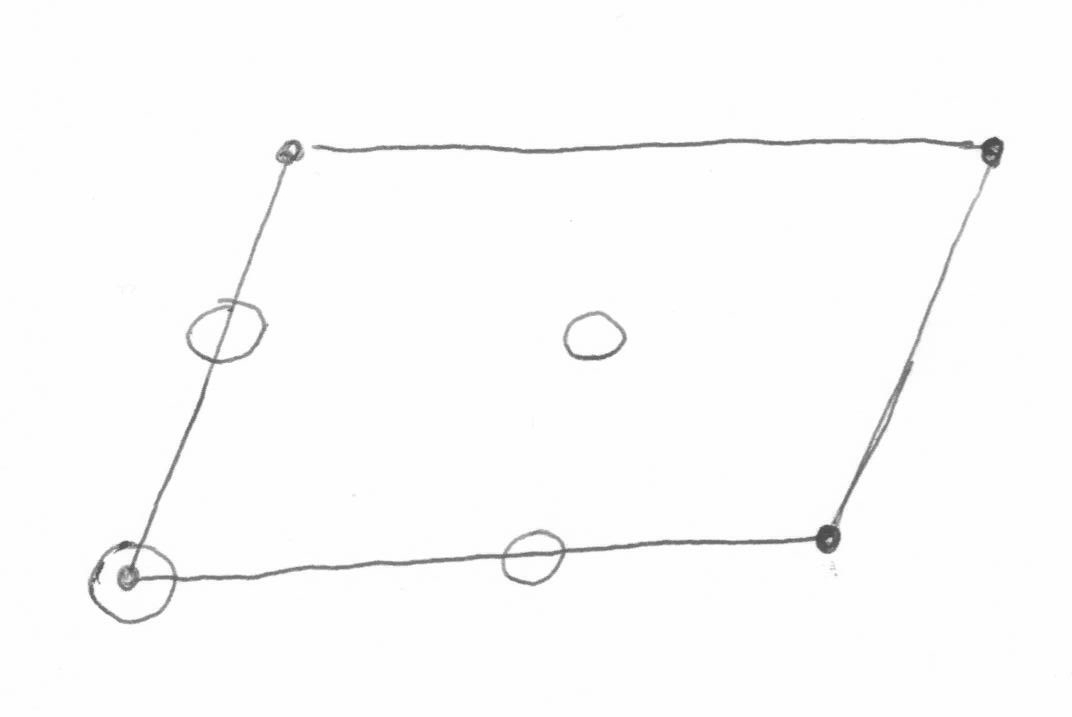
\includegraphics[width=3cm]{lezione-161128-fig1}}

      Allora si ha un solo punto tale che $4x_0^3 - g_2 x_0 - g_3 = 0 (=
      \wp'(z_0))$ e quindi anche questo caso è ok
    \item Se $\wp'(z_0) \neq 0$ allora si ha $z_0 \neq - z_0$ in $T$ e
      quindi $\wp'(z_0) = - \wp'(-z_0)$ poiché la $\wp'$ è
      dispari. Siamo allora nel caso $4x_0^3 - g_2 x_0 - g_3 = \alpha
      \neq 0$ e per avere $y = \pm \sqrt{\alpha}$ posso usare $z_0$ ed
      anche $-z_0$, ovvero ancora una volta la tesi è verificata.
    \end{itemize}
  \end{itemize}

  Per quanto riguarda l'olomorfia, basta aggiungere che la mappa fornita
  $z \mapsto (\wp(z) : \wp'(z) : 1)$ è ovviamente olomorfa tra $T$ e
  $\bbP^2 \bbC$
\end{proof}

\begin{osservazione}
  Notiamo però che se mi viene dato un polinomio di terzo grado nella
  forma $y^2 = 4x^3 - g_2 x - g_3$ non so ancora dire se venga da un
  toro oppure no. Se viene da un toro allora ho la corrispondenza
  biunivoca (proposizione precedente) $\sfrac{\bbC}{L} \leftrightarrow T$
\end{osservazione}

\begin{osservazione}
  Se abbiamo un polinomio in due variabili $f(x, y) = 0$ abbiamo una
  superficie di Riemman, ma non avevamo dimostrato (nel caso delle
  cubiche) la connessione, che in generale non è ovvia.

  Nel caso delle cubiche ciò segue dalla proposizione appena dimostrata.
\end{osservazione}

\paragraph{Altra dimostrazione della connessione} Dimostriamo ancora una
volta che $\ol{E}(\bbC)$ è connesso, iniziando dalla connessione di
$E(\bbC)$ (spazio dei punti affini)

% $x \mapsto 4x^3 - g_2 x - g_3$

La funzione di proiezione $E(\bbC) \rar \bbC$ definita da $(x, y) \mapsto x$ 
diventa un rivestimento tolte le tre radici $\alpha, \beta, \gamma$ del
polinomio $4x^3 - g_2 x - g_3$.

\notamargine{L'idea è che, tolte le radici, abbiamo un rivestimento di
  grado due. I punti del rivestimento si riescono a connettere ``facendo
  dei giri attorno alle radici''}

\begin{center}
  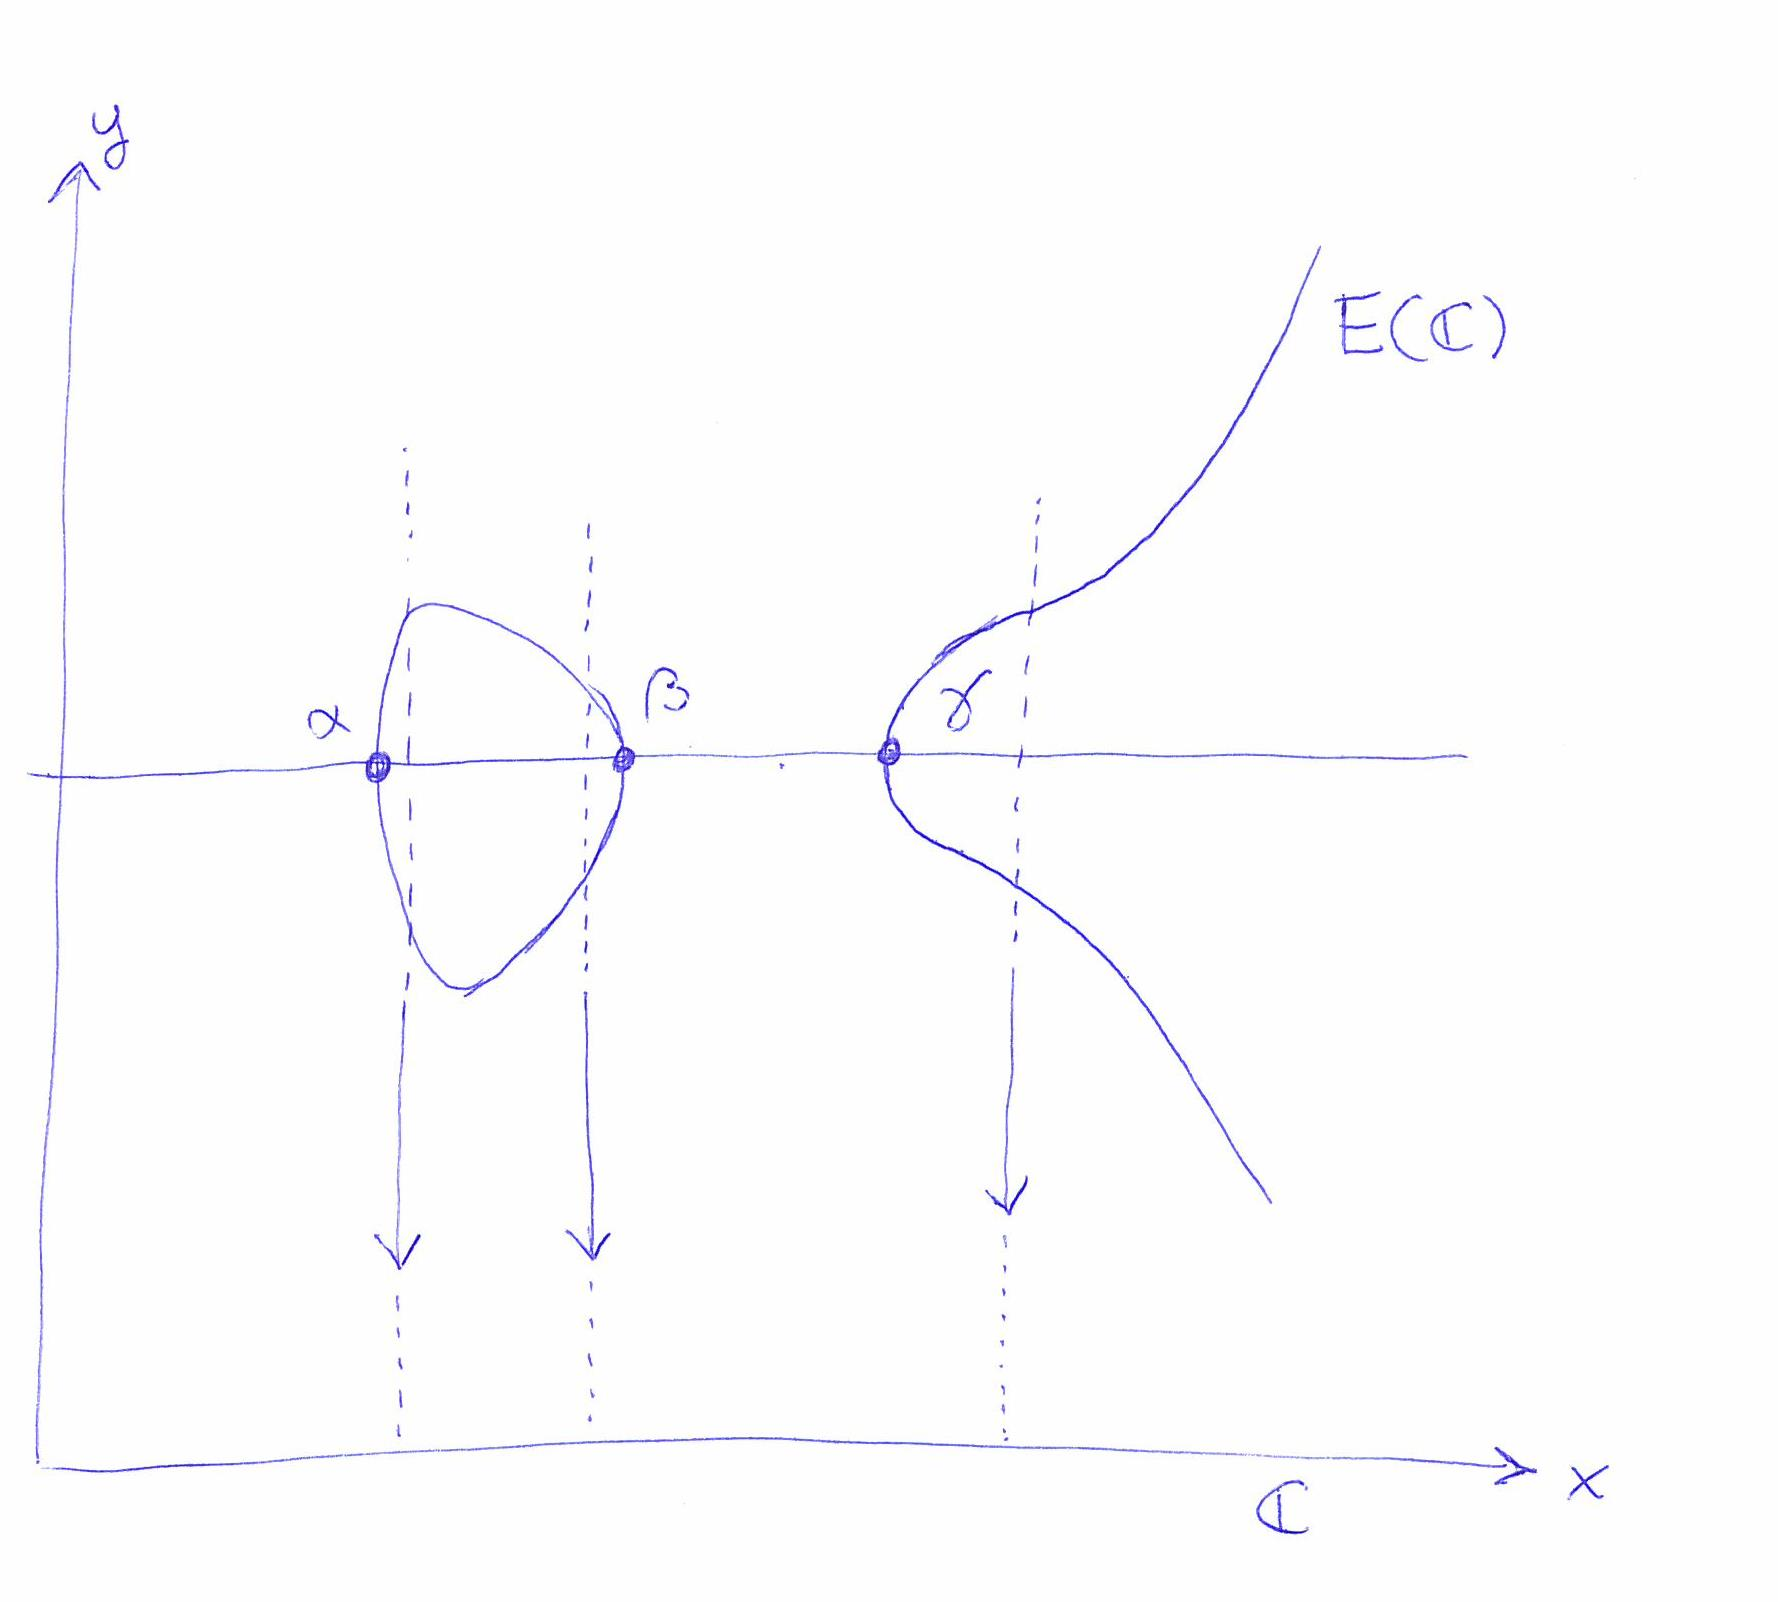
\includegraphics[width=8cm]{lezione-161128-fig1bis}
\end{center}

\notamargine{Per dimostrare che è un rivestimento, possiamo utilizzare
  il fatto che le proiezioni sono mappe aperte e che il numero di punti
  $(x, y) \in E(\bbC)$ che si proiettano su $x$ sono, per
  $x \neq \alpha, \beta, \gamma$, esattamente due, ovvero quelli che
  risolvono $y^2 = 4x^3 - g_2 x - g_3$ con $x$ fissato}

Ovviamente si ha che, avendo il rivestimento grado due, o è connesso,
oppure ha due componenti connesse. Ora, se facciamo un cammino tra due
punti $x_0$ ed $x_1$ del $\bbC$ ``che viene ricoperto'' posso sollevare
il cammino, perché ho un rivestimento. Per mostrare la connessione del
rivestimento basta quindi dimostrare che la fibra di $x_0 \neq \alpha,
\beta, \gamma$ ``è connessa'', ovvero ho un cammino che connette i due
elementi della fibra.

\begin{center}
  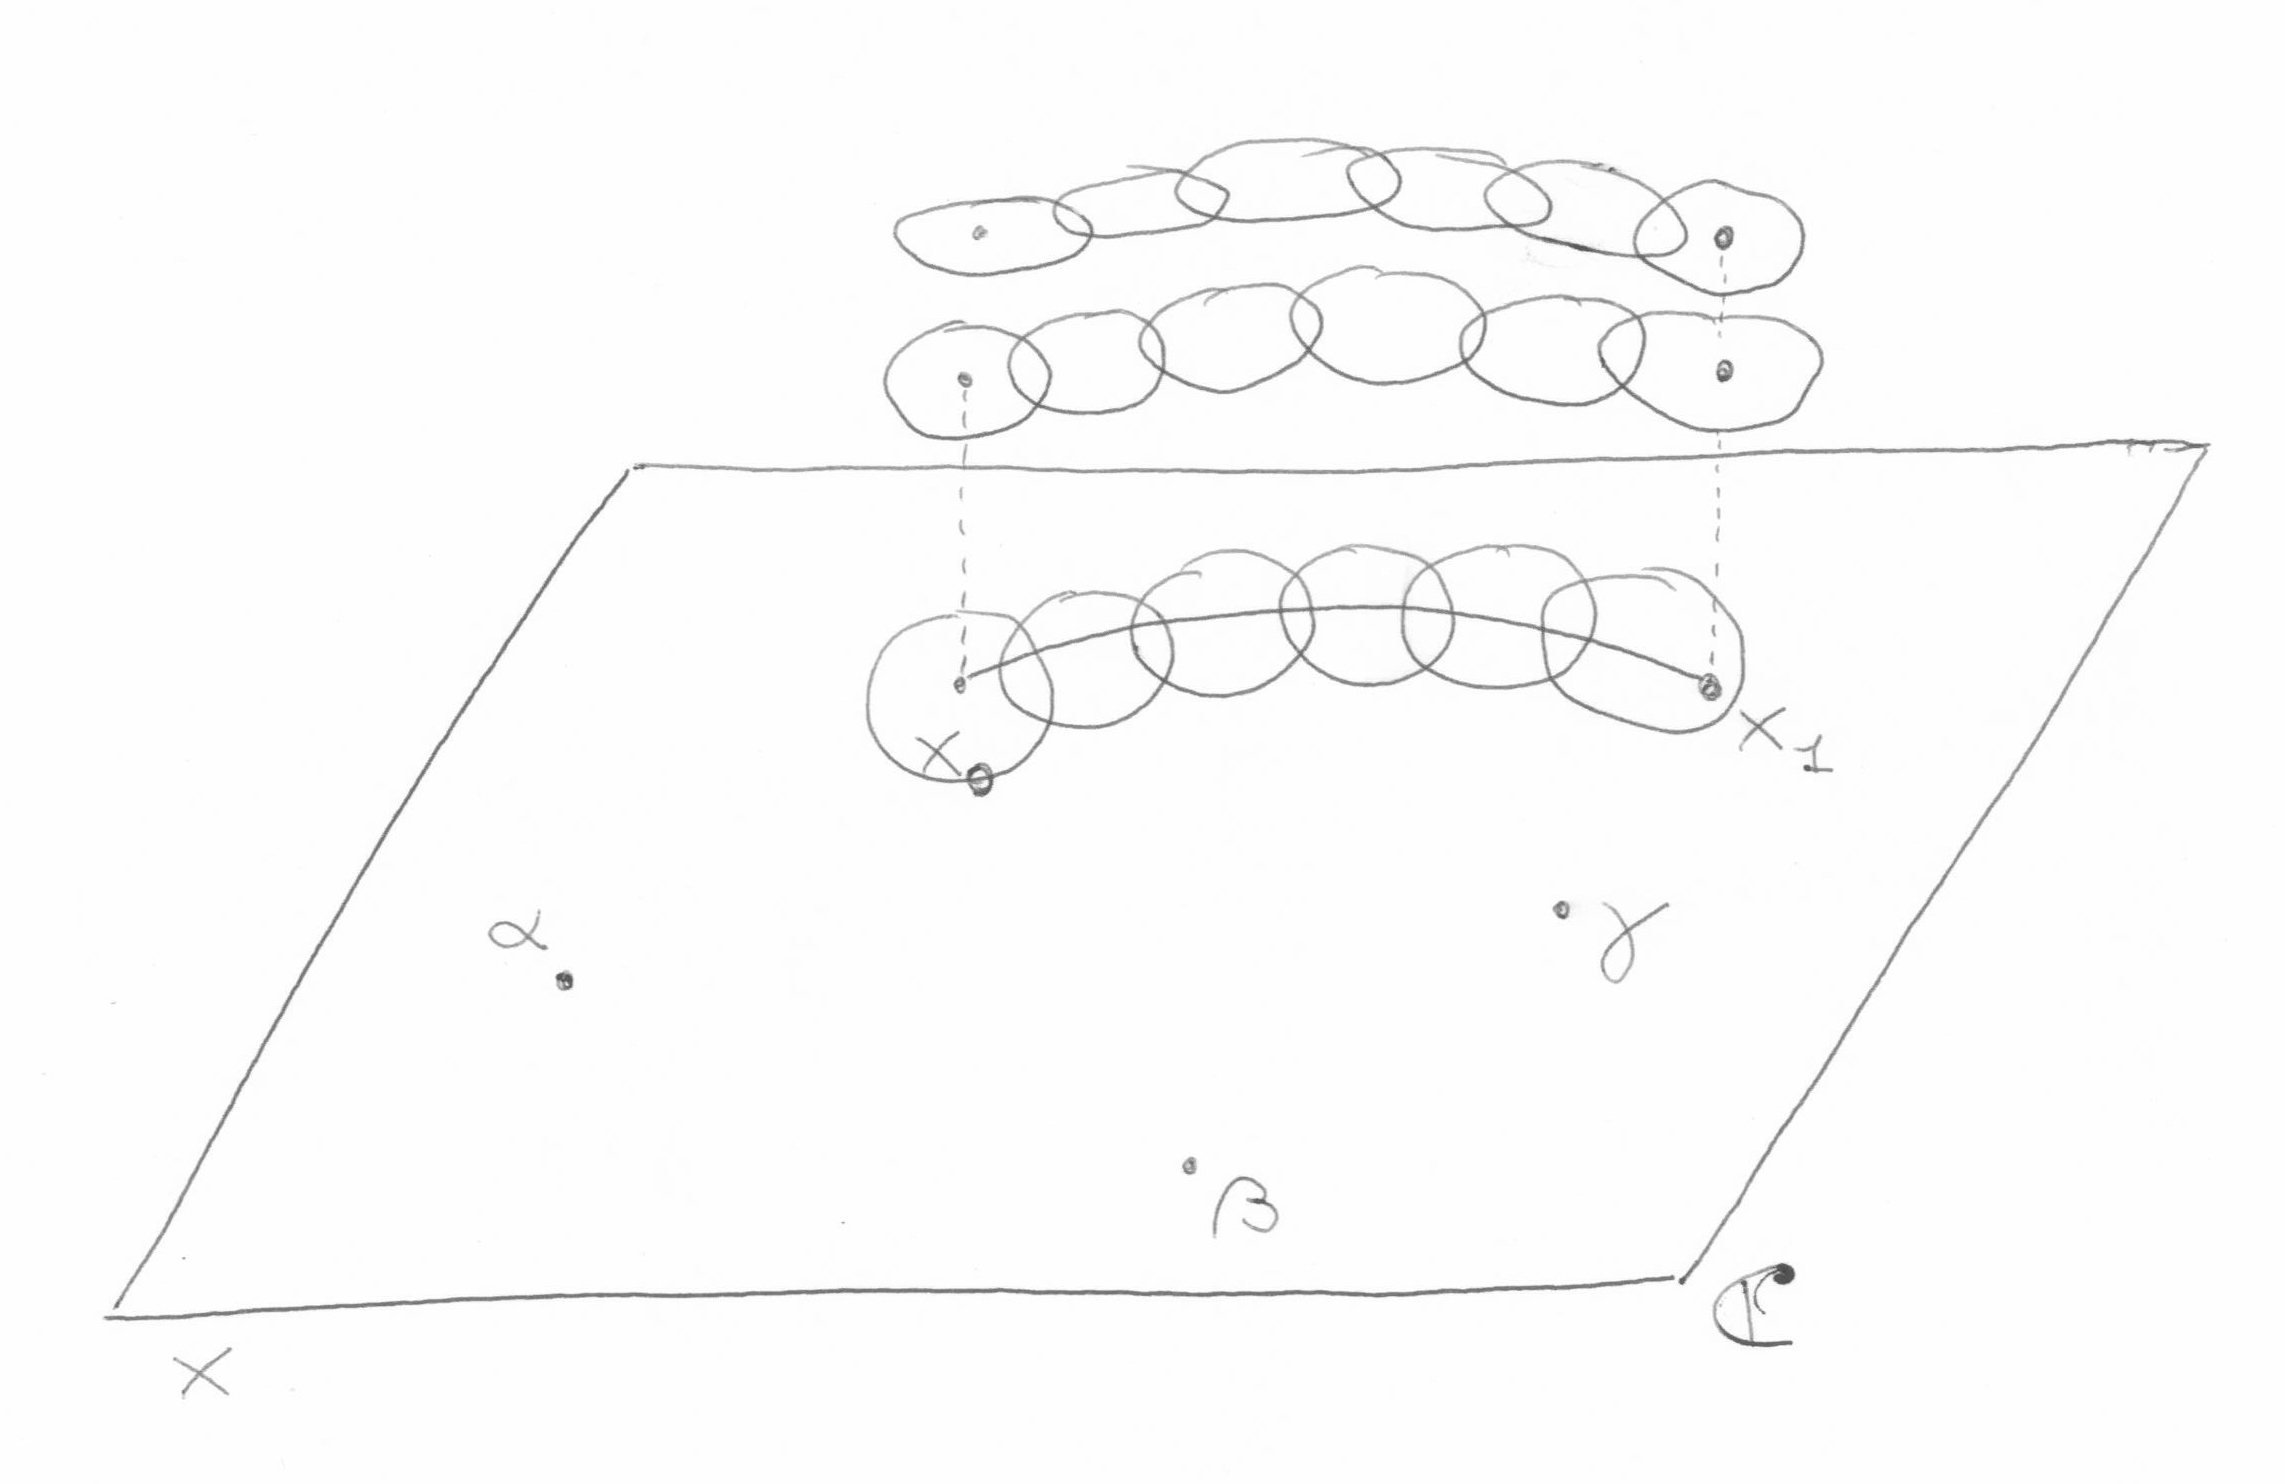
\includegraphics[width=8cm]{lezione-161128-fig2}
\end{center}

Ciò è molto semplice da fare con la radice quadrata: prendiamo infatti
un punto $x_0$ vicino ad $\alpha$. Allora si ha che
$\sqrt{f(x)} = (x - \alpha)^{\frac{1}{2}} \cdot g(x)$ con $g(x)$
olomorfa vicino ad $\alpha$ (poiché siamo lontani da $\beta$ e da
$\gamma$)

Scegliamo una determinazione della radice e facciamo un giro attorno ad
$\alpha$ tornando sulla fibra di $x_0$ ma con valore del segno cambiato.

\notamargine{In particolare si può scegliere un cerchio di raggio
  piccolo (cammino $t \mapsto x_0 + \rho e^{2\pi i t}$) e fare
  esplicitamente il conto ricordando che $z^\frac{1}{2}$ è definito con
  una determinazione di $e^{\log(\frac{1}{2} z)}$}

\section{Cubiche di $\bbP^2\bbC$}
Consideriamo tutte le cubiche in $\bbP^2\bbC$: esse sono definite da
un'equazione omogenea di grado tre $F(x, y, z) = 0$. Mostreremo ora che
nel caso la cubica è parametrizzabile se e solo se è singolare.

\notamargine{Ricordiamo che per parametrizzazione intendiamo una
  isomorfismo birazionale con $\bbP^1$, ovvero una funzione razionale
  $f: \bbP^1 \rar E$ che si intende definita da quasi tutti i punti di
  $\bbP^1$ a quasi tutti i punti di $E$. (Quasi tutti significa tutti
  tranne al più un numero finito)}

\subsection{Caso singolare}
Sappiamo che esiste un punto singolare (ovvero che appartiene alla curva
e su cui tutte le derivate parziali dell'equazione definente la curva si
annullano, ovvero in cui la dimensione del tangente è due).

Allora, se intersechiamo la cubica con il fascio di rette passante per
il punto singolare otteniamo la parametrizzazione (per esercizio
mostrare che ogni retta incontra esattamente un punto della chiusura
proiettiva della cubica e che, ovviamente, dato ogni punto della cubica
esiste una retta che passa per lui e per il punto singolare). La cubica
è quindi parametrizzabile.

\notamargine{Inoltre di punti singolari ne ha al più uno: se ve ne
  fossero due $p, q$ posso tracciare la retta passante per $p$ e per
  $q$, che intersecherebbe la cubica con molteplicità quattro.}

\subsection{Caso non singolare}
In ogni cubica c'è sempre un punto di flesso (ovvero dove l'hessiano si
annulla). Usando una proiettività si può mandare il flesso nel punto
all'infinito $(0 : 1 : 0)$.

\notamargine{L'Hessiano in questo caso è il determinante della matrice
  hessiana del polinomio che definisce la cubica, ovvero
  $\Det (\frac{\partial F}{\partial x_i \partial x_j})_{i, j = 1, 2, 3}$

  Il polinomio hessiano ha, per un facile conto, grado $3 (d-2)$, dove
  $d$ è il grado della curva $F$, oppure è identicamente nullo.
  Nel primo caso, per il teorema di Bèzout, esistono punti di $\bbP^2$
  su cui esso si annulla assieme all'equazione di $F$, ovvero esistono
  punti di $F$ di flesso (e sappiamo anche che sono $3 (d - 2) d$
  contati con molteplicità)}

Facendo i conti con il flesso all'infinito e con tangente al flesso la
retta $\{ z = 0 \}$ ottengo un'equazione simile a quella di Weierstrass
a cui si arriva con alcune manipolazioni algebriche:
$y^2 = 4 x^3 - a x - b$.

Se poi effettuiamo la trasformazione $x \mapsto \lambda^2 x$ e $y
\mapsto \lambda^3 y$ con $\lambda \neq 0$ allora si ottiene $y^2 = 4 x^3
- \frac{a}{\lambda^4} x - \frac{b}{\lambda^6}$.

Posso quindi scegliere $\lambda$ in modo da far scomparire un parametro.

\begin{osservazione}
  Non sappiamo ancora che ogni cubica viene da un toro, quindi non
  potevamo dire a priori che lo spazio delle cubiche ha un solo
  parametro.
\end{osservazione}

Che succede se al posto di un reticolo $L$ ne prendiamo uno omotetico
$\lambda L$ con $\lambda \in \bbC^*$? Le funzioni $g_2$ e $g_3$ si
trasformano nel seguente modo:
$ g_2 \mapsto \frac{g_2}{\lambda^4} ,\quad g_3 \mapsto
\frac{g_3}{\lambda^6}$ e quindi l'equazione della cubica diventa:
$E_{\lambda L}: y^2 = 4x^3 - \frac{g_2}{\lambda^4} x -
\frac{g_3}{\lambda^6}$

Quali sono le funzioni razionali di $a$ e di $b$ che rimangono
invarianti per trasformazioni omotetiche? Sicuramente vi è
$\frac{a^3}{b^2}$.
\notamargine{Per esercizio si può dimostrare che ogni funzione razionale
  invariante per omotetia di $a$ e di $b$ si scrive come funzione
  razionale di $\frac{a^3}{b^2}$}

Dato un reticolo $L$, lo scriviamo come $\bbZ \tau + \bbZ$ con $\tau \in
\cH$ (semipiano superiore) a meno di rotomotetie del piano.

\begin{proposizione}
  $\frac{g_2^3}{g_3^2}$ è una funzione di $\tau$ non costante e meromorfa
\end{proposizione}

Per quanto riguarda la meromorfia, si può notare che, definita la somma
$$S_n = \sum_{(r, s) \in \bbZ^2 \setminus \{(0, 0)\}} \frac{1}{(r \tau
  + s)^n}$$ essa converge per $n \ge 2$ e definisce una funzione olomorfa
di $\tau$. Segue quindi che, se $S_3$ non è identicamente nulla, si ha
che $\frac{g_2^3}{g_3^2} = \frac{S_2^3(\tau)}{S_3^2(\tau)}$ per
definizione e quindi la succitata funzione è meromorfa.

\notamargine{Per verificare la convergenza assoluta della sommatoria per
  $n > 2$ si può maggiorare la serie dei valori assoluti con l'opportuno
  integrale in due variabili. Per il caso $n=2$ non saprei...}

Inoltre, se trovassimo due reticoli $L_1$ ed $L_2$ in cui valga
rispettivamente
$$g_3(L_1) = 0, g_2(L_1) \neq 0$$
$$g_2(L_2) = 0, g_3(L_2) \neq 0$$
ne seguirebbe che la funzione non è costante.

Si possono a tal proposito considerare i reticoli $\tau = i$ e
$\tau = \zeta_3$:
\begin{itemize}
\item ($\tau = i$) Sia $L_1 = \bbZ[i]$. Allora si nota che $i L_1 = L_1$
  e quindi si ha $g_2(i L_1) = g_2(L_1)$ e per omogeneità
  $g_3(L_1) = g_3(i L_1) = i^{-6} g_3(L_1)$ da cui segue $g_3(L_1) = 0$.

  Inoltre $g_2 \neq 0$, altrimenti il polinomio definente avrebbe radici
  multiple (segue direttamente dall'equazione del polinomio).

\item ($\tau = \zeta_3$) Sia $L_2 = \bbZ[\zeta_3]$ e notiamo che
  $\zeta_3 L_2 = L_2$ che implica $g_2(L_2) = g_2(\zeta_3 L_2) =
  \zeta_3^4 g_2(L_2) = \zeta_3 g_2(L_2)$ e quindi $g_2(L_2) = 0$
\end{itemize}


\thislesson{30 Novembre 2016}{Collegamenti tra tori e curve ellittiche}

	Se ho una mappa $\phi: X \rar Y$, bigettiva e olomorfa tra superfici di Riemann, allora non è necessariamente biolomorfa.
	
	Infatti sia $C = \{ (x,y) \in \bbC^2 : y^2=x^3 \}$, e sia $\tilde C$ il suo completamento proiettivo. Allora detta $\phi: \bbP^1 \rar \tilde C$ la mappa $ (t : 1) \mapsto (t^2 : t^3 : 1)$ e $(1 : 0) \mapsto (0:1:0)$ questa è chiaramente bigettiva e olomorfa.

	Tuttavia l'inversa è data da $(x:y:1) \mapsto (\frac yx:1)$, che non è olomorfa in quanto il differenziale in $(0:0:1)$ è nullo (ma non è localmente costante).
	
	Il problema scaturisce dal fatto che il polinomio ha una radice doppia.
	
	Tuttavia se aggiungiamo che il differenziale sia full rank allora necessariamente deve essere biolomorfa.
	\begin{proof}
		Consideriamo il seguente diagramma:
		\[
		\begin{diagram}
			X & \rTo^\phi & Y \\
			\dTo>a & & \dTo>b \\
			\Omega_1 & \rTo^\psi & \Omega_2
		\end{diagram}
		\]
		
		$a, b$ sono le rispettive proiezioni in carta, quindi hanno differenziale full-rank. Segue che la composizione $\psi = b\circ \phi \circ a^{-1}$ ha anch'essa differenziale full-rank.
		Ora non capisco cosa stia cercando di scrivere formlmente, ma l'idea è che se ho il differenziale full-rank allora per il teorema di invertibilità locale posso trovare un'inversa differenziabile, e che soddisferà le condizioni per essere olomorfa. %TODO fare meglio% 
	\end{proof}

	\begin{proposizione}
		La mappa di Weierstrass $\wp$ è biolomorfa. 
	\end{proposizione}
	\begin{proof}
		Abbiamo già visto che la $\wp$ è olomorfa e biiettiva, manca da dimostrare che l'inversa è olomorfa.
		Per questo mi basta guardare che il differenziale sia mai nullo. D'altra parte il differenziale della mappa di Weierstrass è $ (\wp'(z), \wp''(z))$ che non è mai nullo (Se abbiamo $\wp'(z_0) = \wp''(z_0) = 0$ vuol dire che $\wp'$ ha uno zero doppio in $z_0$, ma noi conosciamo già tutti gli zeri di $\wp'(z_0)$, che sono sui punti di $L/2$ diversi dall'origine).
	\end{proof}
	
	Grazie a questo possiamo dire che la curva ellittica ha la stessa struttura complessa del toro da cui proviene (se proviene effettivamente da un toro, cosa che si rivelerà vera).
	
	\begin{osservazione}
		Nonostante non abbia capito cosa c'entra, sul toro esiste una forma differenziale globale data da $dz$. Grazie alla mappa di Weierstrass, posso trasportarla sulla cubica e diventa $\frac{dx}y$, e segue che questa non ha poli, neanche all'infinito.
	
	\end{osservazione}

        \notamargine{Mostriamo questa affermazione sui differenziali: nella parametrizzazione di Weierstrass, si ha che $x = \wp(z)$ e $y = \wp'(z)$. Allora, chiamata $g: E \rar \bbC$ l'inversa della parametrizzazione si ha che $g_*(\frac{dx}{y}) = \frac{d(\wp(z))}{\wp'(z)} = \frac{\wp'(z) dz}{\wp'(z)} = dz$}
        
	\section{Discriminante}
	
	Ricordiamo che per una cubica del tipo $y^2=p(x)$ la non singolarità equivale all'assenza di radici multiple. Un modo rapido per vedere se un polinomio ha radici multiple è definire il discriminante.
	
	Sia quindi $f(t)$ un polinomio con radici $\alpha_i$ (eventualmente ripetute), definiamo $D_t=\prod_{i<j} (\alpha_i - \alpha_j)^2$. Questo è simmetrico nelle radici pertanto lo posso scrivere come un polinomio a coefficienti interi nei coefficienti di $f$.
	
	Se $\deg f=2$: $D_t= b^2-4ac$. Calcoliamolo ora per $\deg f=3$.

	Prendo $f(t)=t^3+At+b$. Essendo $D_t$ di grado 6 nei coefficienti, deve essere combinazione linerare di $A^3$ e $B^2$. Ora mettendomi nel caso particolare $A=0,B=-1$ e nel caso $B=0$ posso agilmente scoprire che 
	\[
		D_t=-4a^3-27B^2
	\]
	
	\section{Studio delle cubiche al variare di $\frac{a^3}{b^2}$}
	
	Sappiamo che ogni cubica non singolare è isomorfa a $y^2=x^3-ax-b$ mediante trasformazioni affini.
	
	Considero il parametro $\frac{a_3}{b^2}$. Sappiamo che è invariante per le omotetie del tipo $x\mapsto \lambda^2x, y\mapsto\lambda^3y$. Ho però il problema che esso non è definito per $b=0$.

	Utilizzo quindi il discriminante. So che dato che il polinomio non ha radici multiple, il discriminante sarà non nullo: sfrutto questa informazione per considerare come parametro una funzione che dipenda solo da $\frac{a^3}{b^2}$ che abbia il discriminante come denominatore. Uso quindi
	
	\[
		j = c \cdot \frac {a^3}{a^3-27b^2}
	\]

	Convenzionalmente, invece dell'ovvia $c=1$ si pone $c=1728$ per qualche oscuro motivo.
	
	Mostriamo ora che una cubica proveniente da un toro non ha radici multiple.
	
	\begin{proof}
		Sappiamo che 
		\[
			\wp'(z)^2=4\wp(z)^3-g_2\wp(z)-g_3 = 4(\wp(z)-e_1)(\wp(z)-e_2)(\wp(z)-e_3)
		\]
		
		Quindi $\wp(z_0)=e_i \Rar\wp'(z_0)=0$.
		Se $L=\bbZ\omega_1 + \bbZ\omega_2$, allora $\wp'(z)$ si deve annullare su tutti i punti di $\frac L2$: infatti se $l \in \frac L2$ allora $l \equiv -l \pmod L$, e dato che $\wp'(z)$ è dispari ho che 
		\[
			\wp(l) = \wp(-l) = -\wp(l)
		\]
		
		Visto sul toro, $\wp'(z)$ si annulla in quattro punti.
		
		E invece no! Ho mentito. Nell'origine non si annulla, c'è un polo. Dato che $\wp'(z)$ ha esattamente un polo di ordine tre, allora ho trovato tutti gli zeri, che sono $\frac{\omega_1}2, \frac{\omega_2}2, \frac{\omega_1+\omega_2}2$.
		
		%TODO manca da dire perché sono davvero distinte, che non sto ben capendo
                % Sono distinte perché se ho om1/2 = om2/2 ==> om1 = om2 assurdo perché i generatori del reticolo sono distinti
                % Il caso om1/2 = (om1+om2)/2 ==> om2 = 0 assurdo perché so che devono generare un reticolo di rango due

	\end{proof}

	Ora vediamo che tori con la stessa $j$ sono omotetici.
	
	\begin{proof}
          Suppongo che $T, T'$ abbiano la stessa $j$. Allora ho $\frac{a^3}{b^2}=\frac{a'^3}{b'^2}$. Quindi se con un omotetia faccio in modo che $a$ venga mandato in $a'$, allora sicuramente $b$ viene mandato in $b'$ oppure in $-b'$.

          Osserviamo che le due cubiche che in forma normale di Weierstrass hanno come parametri $a, b$ e $a, -b$ sono in realtà la stessa curva. Infatti applicando la trasformazione $x' = -x$, $y' = iy$ si ha $y^2 = 4x^3 - ax - b \mapsto - y'^2 = - 4x'^3 + ax - b$ che coincide con la forma $y'^2 = 4x'^3 - ax - (-b)$.
		
          Quindi sia $T$ che $T'$ sono biolomorfi alla stessa curva, quindi sono biolomorfi tra loro e dunque omotetici.
	\end{proof}
	
	\begin{osservazione}
		$j(\tau)$ è una funzione non costante e olomorfa. Vedremo anche che è suriettiva.
	\end{osservazione}


%% Lezione di esempio. Copiate questo file nella lezione che dovete creare
%%----------------------------------------------------------------------------------------------------------------------------------------------------------------------------------------------------------------------------------------------------- per avere già uno scheletro di come scrivere le lezioni

%% Diamo un nome al capitolo. Idealmente mettiamo la data della lezione ed
%% una sua breve descrizione / argomenti trattati
\chapter{05 Dicembre 2016 - Campi di funzioni, Estensioni di mappe razionali a mappe olomorfe}
\justify

\section{Campi di funzioni}

Sia $E: y^2=4x^3-ax-b$ una cubica non degenere su $\bbC$.
Siano $x,y:E\rightarrow\bbC$ le funzioni proiezione su $\bbC$, definite sulla cubica.
\begin{definizione}
Indico con $\bbC(t)$ le funzioni razionali in una variabile, quindi $4t^3-ax-b$ è un elemento di $\bbC(t)$, perciò sia $u$ radice quadrata di $f(t)=4t^3-at-b$ e sia $\bbC(t,u)$ l'estensione di $\bbC(t)$ con $u$.\\
Siano inoltre $\bbC(x)$ e con $\bbC(x,y)$ i campi delle funzioni razionali sulle $x$ e $y$ appena definite, che quindi sono funzioni con dominio $E$ e codominio $\bbC$.
\end{definizione}

\begin{osservazione}
Si noti che $\bbC(t)\subseteq\bbC(t,u)$ è un'estensione di grado $2$.\\
Si noti che $\bbC(x)$ è un sottoinsieme delle funzioni razionali di una variabile, calcolate poi in $x$. In particolare è il sottoinsieme delle funzioni razionali in una variabile con denominatore che è non zero se calcolato in $x$, calcolate in $x$. Quindi lo si può pensare come un sottoinsieme delle funzioni razionali non definite in qualche punto.
Analogo per $\bbC(x,y)$.
\end{osservazione}

\begin{proposizione}
$\bbC(x)\cong_{\bbC}\bbC(t)$
\end{proposizione}

\begin{proof}
Considero la mappa $t\mapsto x$ che lascia fisso $\bbC$, si ha che è ben definito poiché l'immagine di una funzione razionale $R(t)$ è una funzione definita tranne in un numero finito di punti, si ha che è surgettivo e omomorfismo di campi, inoltre siccome è non nullo è iniettivo.
\end{proof}

\begin{proposizione}
$\bbC(x,y)\cong_{\bbC}\bbC(t,u)$
\end{proposizione}

\begin{proof}
Considero la mappa $t\mapsto x, u\mapsto y$ che lascia fisso $\bbC$, per vedere che è ben definito bisogna mostrare che se $R(t,u)=S(t,u)$ allora $R(x,y)=S(x,y)$, ma sottraendo mi riduco a mostrare che se $R(t,u)=0$ allora $R(x,y)=0$, ma $R(t,u)$ è $0$ solo se è divisibile per $u^2-f(t)$, ma nell'immagine $y^2-f(x)$ è $0$. Per ESERCIZIO si verifichi che è un omomorfismo e che l'immagine sta dentro $\bbC(x,y)$
\end{proof}

\begin{osservazione}
Si ha che $\bbC(x)\subseteq\bbC(x,y)$ è di grado $2$ quindi gli elementi di $\bbC(x,y)$ si possono rappresentare come $\{ R(x)+y S(x) | R,S \in \bbC(x)\}$.
\end{osservazione}

Ci si chiede se $\bbC(x,y)$ è isomorfo a un certo $\bbC(w)$.
Se lo fosse allora si avrebbe che $x=f(w), y=g(w)$ con $f$ e $g$ razionali, quindi la curva sarebbe parametrizzabile. "Si noti che qui c'è un forte collegamento tra concetti algebrici (campo semplice) e geometrici (parametrizzabilità) (questo si vedrà meglio più avanti nel corso)".

\begin{osservazione}
Non si può usare il teorema dell'elemento primitivo per l'estensione $\bbC\subseteq\bbC(x,y)$ infatti $x$ è trascendente su $\bbC$.
\end{osservazione}

\begin{proposizione}Se la cubica proviene da un toro ( $a=g_2(L), b=g_3(L)$ ) allora $\bbC(x,y)\cong_{\bbC}\bbC(\wp(z),\wp'(z))$.
\end{proposizione}

\begin{proof}
Si noti che quest'ultimo è un campo di funzioni meromorfe, infatti i polinomi nelle $\wp(z)$ e $\wp'(z)$, se non sono nulli, si annullano solo in un numero finito di punti (altrimenti gli zeri hanno un punto di accumulazione). Quindi presi due polinomi $P$ $Q$ calcolati in $\wp(z)$ e $\wp'(z)$ si ha che il loro quoziente $P/Q$ è nullo solo se il denominatore è nullo quindi solo in un numero finito di punti. Per ESERCIZIO si costruisca l'isomorfismo $\bbC[x,y]\rightarrow\bbC[\wp(z),\wp'(z)]$ e poi si passi ai quozienti completando la dimostrazione.
\end{proof}


\section{Estensioni di mappe razionali}
Sia $E'$ un'altra cubica dello stesso tipo di $E$.

\begin{definizione}
Una mappa razionale $E\rightarrow E'$ è una mappa $E\rightarrow E'$ definita su "$\tilde{E}$ meno un numero finito di punti" e che può scrivere in termini razionali di $x$ e $y$, cioè $\varphi(x_0,y_0)=(\varphi_1(x_0,y_0),\varphi_2(x_0,y_0) )$ con $\varphi_1$ e $\varphi_2$ razionali.
\end{definizione}

\begin{osservazione}
Per finire in $E'$ si deve avere che $\varphi_2^2=4\varphi_1^3-a'\varphi_1-b'$, quindi non è facile trovarne nemmeno dalla curva in se stessa. Qualche volta non ce ne sono (a parte le costanti, ovviamente) (vedi quanto scritto sotto per i tori, per aiutarti ad avere un esempio)
\end{osservazione}

Se considero una funzione da un toro in $\bbC$ meromorfa (quindi non definita sul tutto il toro, la chiama così per abbreviare) allora si può estendere ad una funzione olomorfa dal toro verso $\bbP^1(\bbC)$.
Quindi se la curva $E$ proviene da un toro e $E'=\bbC$ posso estendere la mappa razionale a tutta $\tilde{E}$, a valori in $\bbP^1(\bbC)$.
Questo si può fare anche se in arrivo non c'è $\bbC$, ma una qualsiasi $E'$, considerando come codominio della funzione dalla curva estesa $\tilde{E'}$.

\begin{proposizione}
Una mappa razionale $E\rightarrow E'$ si estende ad una mappa olomorfa $\tilde{E} \rightarrow \tilde {E'}$.
\end{proposizione}

\begin{proof}
Basta dimostrare che una mappa razionale $E\rightarrow \bbC$ si estende a $\tilde{E}\rightarrow\bbP^1(\bbC)$ (il caso generale è analogo, ha detto).\\
Ho quindi una mappa da $\tilde{E}$ meno un numero finito di punti a $\bbC$ olomorfa e devo dimostrare che in questi punti NON ha una singolarità essenziale. Siccome i punti mancanti sono in numero finito riesco a trovare per ogni punto un intorno $U$ dove la funziona è definita su tutto $U-\{ p_0\}$ e una carta $\varphi:U\rightarrow \Omega\subseteq\bbC$, in cui suppongo che $\varphi(p_0)=0$ per semplicità. Allora esiste $\psi:\Omega-\{ 0\}\rightarrow U$ con $\varphi(0)=p_0$ tale che $\varphi\circ\psi:\Omega-\{ 0\}\rightarrow \bbC$ è olomorfa. ( $\psi$ è ottenuta con il Teorema del Dini come inversa delle funzioni coordinate, nel modo visto in altre lezioni).\\
Ci basta dimostrare che la mappa $\varphi\circ\psi$ ha al più un polo in $0$.
Supponiamo per assurdo che $0$ sia una singolarità essenziale, allora per il teorema di Weierstrass ogn intorno bucato di $0$ ha immagine densa in $\bbC$. Sia quindi $V_n$ una successione numerabile di dischi aperti bucati di centro zero e raggio $2^{-n}$. Per il Teorema di Baire si ha che l'intersezione delle immagini dei $V_n$ (le mappe olomorfe sono aperte) è un denso, che chiamo $A$.\\
Sia quindi $\xi\in A$, si ha che $\forall n \exists z_n\in V_n - \{ 0 \} : \varphi ( \psi(z_n ))=\xi$, quindi gli $z_n$ formano una successione tendente a $0$. Ne segue che gli $z_n$ sono almeno una quantità numerabile e siccome $\psi$ è una bigezione anche gli $\psi(z_n)$ sono una quantità almeno numerabile. Ne segue che la fibra $\psi^{-1} (\xi )$ è almeno numerabile, ma ciò è assurdo, poichè $\varphi$ è una mappa razionale (nota che se $\varphi$ è costante non c'è un assurdo, ma sappiamo estendere le mappe costanti). Quindi non ci può essere una singolarità essenziale.
\end{proof}

\notamargine{
Teorema di Baire: In uno spazio metrico completo l'intersezione numerabile di aperti densi è densa. 
Oppure: if a non-empty complete metric space is the countable union of closed sets, then one of these closed sets has non-empty interior. (entrambe da Wikipedia) }

\begin{osservazione}
Nota che la dimostrazione fatta vale per qualsiasi curva algebrica che sia una Superficie di Riemann.\\
Nota che l'abbiamo dimostrato in 2 modi, uno usando che le curve ellittiche vengono dai tori (in modo apparentemente semplice, ma che richiede tanta teoria sotto) e uno usando Baire, che è un teorema semplice.\\
Si potrebbe dimostrare in un altro modo puramente algebrico usando che certi anelli di coordinate sono principali, quest'ultima dimostrazione è complicata ma ha il pregio di valere anche in ambiti in cui la caratteristica è un primo $p$.
\end{osservazione}

Come abbiamo già detto è difficile trovare mappe razionali, osserviamo che se due cubiche $E$ e $E'$ provengono da due tori $T$ e $T'$ si ha che ogni mappa razionale $E\rightarrow E'$ induce una mappa olomorfa sui completamenti quindi induce una mappa olomorfa $T\rightarrow T'$. Nota che (come visto alla "lezione del 24 Ottobre") queste mappe sono, a meno di una traslazione, delle moltiplicazioni per costanti, viste su $\bbC$. E che deve valere la relazione tra i reticoli $\mu L\subseteq L'$, condizione molto restrittiva.

\begin{proposizione}
Esiste un algoritmo per dire se esiste una mappa razionale non costante tra due cubiche, se si conoscono stime a priori sul grado della funzione razionale.
\end{proposizione}

\begin{proof} La mappa razionale è una mappa del tipo $(\varphi_1,\varphi_2)$ con $\varphi_i=r_i(x)+y s_i(x)$ $i=1,2$  che deve soddisfare $(r_2(x)+y s_2(x))^2=4(r_1(x)+y s_1(x))^3-a'(r_1(x)+y s_1(x))-b'$, separando i termini in $1$ e $y$ si ricavano due identità nella sola variabile $x$. Qualcosa del tipo $A(x,r_1,r_2,s_1,s_2)=0$ e $B(x,r_1,r_2,s_1,s_2)=0$. Che ci sono algoritmi per capire se questo sistema ha soluzione, se si conoscono delle stime sui gradi.
\end{proof}

\begin{osservazione} Esiste un algoritmo recente per stimare a priori i gradi delle $r_i$ e $s_i$.\\
Esiste un teorema(profondo): Se ne esiste una non costante allora ne esiste una con grado limitato.\\
Nota che le condizioni sui reticoli sono condizioni con quantità trascendenti, difficili da verificare (equivale a chiedersi se delle espressioni che riportano serie infinite (la $\wp$) sono numeri razionali (???))
\end{osservazione}

\chapter{7 Dicembre 2016 - Legge di Gruppo sulla cubica e Gruppo dei Divisori}
\justify

\section{Legge di gruppo sulla cubica}
Abbiamo già visto che con la proiezione al quoziente $\pi : \bbC \rightarrow T$ il toro eredita la struttura di gruppo additivo da $\bbC$.
Vogliamo vedere adesso chi è la legge di gruppo sulla cubica $\widetilde{E}$.
Considero la mappa di Weierstrass: $T\rightarrow \widetilde{E}$ che manda $z \rightarrow (\wp(z):\wp'(z):1)$. Mi chiedo chi sia l'immagine di $z_1 + z_2$.

\begin{teorema}
  \label{leggedigruppo}
  Vale che $\wp(z_1+z_2) = \frac{a^2}{4} - \wp(z_1) - \wp(z_2) $
  con $a = \frac{\wp'(z_2) - \wp'(z_1)}{\wp(z_2) - \wp(z_1)}$.
\end{teorema}

\begin{proof}
Cerco dei coefficienti $a,b$ tali che $\wp'(z_1) - a\wp(z_1) - b$ si annulli in $z_1$ e $z_2$.
Risolvendo ottengo:

\begin{displaymath}
  \left\{
    \begin{array}{l}
      a = \frac{\wp'(z_2) - \wp'(z_1)}{\wp(z_2) - \wp(z_1)} \\
      b = - \frac{\wp'(z_2) \wp(z_1) - \wp'(z_1) \wp(z_2)}{\wp(z_2) - \wp(z_1)} \\
    \end{array}
  \right.
\end{displaymath}

Supponiamo $\wp(z_2) \neq \wp(z_1)$, altrimenti ho due casi: $z_2 \equiv z_1$, che tratterò alla fine, e $z_2 \equiv -z_1$.
In quest'ultimo caso la formula di addizione perde di senso, perché $\wp$ ha un polo in zero.


Considero la funzione $\wp'(z) - a \wp(z) - b$: è una funzione ellittica.

Inoltre, pensata nei complessi, ha poli solo nei punti del reticolo $L$, quindi pensata sul toro ha un polo solo in zero, ed è di ordine 3.
Allora ha 3 zeri, di cui sicuramente due sono $z_1$ e $z_2$. Chiamo $z_3$ l'altro zero.

Un teorema che abbiamo visto (T3) assicura che per le funzioni ellittiche $$ \sum_\text{zeri} z_i - \sum_\text{poli} w_i \equiv 0$$

Nel nostro caso $z_1 + z_2 + z_3 - (0+0+0) \equiv 0$, da cui $z_3 \equiv - z_1 - z_2$.

Imponendo ora che $\wp'(z) - a \wp(z) - b$ si annulli in $ -z_1 - z_2 $, ottengo:
$$ \wp'(-z_1-z_2) - a \wp(-z_1-z_2) - b = 0 $$
Da questo e dalla parità/disparità di $ \wp, \wp' $ segue:
$$ - \wp'(z_1+z_2) = a \wp(z_1+z_2) + b $$
Ora ricordo che: $$ - \wp'(z_1+z_2)^2 = 4 \wp(z_1+z_2)^3 - g_2 \wp(z_1+z_2) - g_3 $$
Mettendo a sistema queste due equazioni si ottiene:
$$4 \wp(z)^3 -a^2 \wp(z)^2 - (2ab+g_2) \wp(z) - g_3 - b^2=0$$
$$\wp(z)^3 -\frac{a^2}{4} \wp(z)^2 - \frac{(2ab+g_2)}{4} \wp(z) - \frac{(g_3 - b^2)}{4}=0$$
nei punti $z_1, z_2, z_3$.

Ovvero, pensandolo come un polinomio in $\wp(z)$, ha come radici $\wp(z_1), \wp(z_2), \wp(z_3)$.
Per le relazioni radici-coefficienti so che: $\frac{a^2}{4} = \wp(z_1) + \wp(z_2) + \wp(z_3)$.

$$\wp(z_1+z_2) = \frac{a^2}{4} - \wp(z_1) - \wp(z_2)$$
che è la formula di addizione che stavamo cercando.


Si può dimostrare che vale per ogni $z_1, z_2$, anche uguali (purché diversi da $0$), si tratta di fare
$$ \lim_{z_1 \rightarrow z_2} \frac{a^2}{4} - \wp(z_1) - \wp(z_2)$$ con De L'Hopital. 
\end{proof}


Notiamo con stupore che è un espressione razionale, cosa che a priori non era ovvia.
In modo analogo si può ricavare una formula di addizione per $\wp'$.

\begin{osservazione}
Ricordando che la mappa di Weierstrass pensata in modo affine è $z \rightarrow (\wp(z),\wp'(z))$, ho quindi dimostrato che la mappa di Weirstrass induce la seguente struttura di gruppo su $E$:
$(x_1,y_1) + (x_2,y_2) = (x_3,y_3)$ con

\begin{displaymath}
  \left\{
    \begin{array}{l}
      x_3 = \frac14 a^2 - x_1 - x_2 \\
      y_3 = - ax_3 - b \\
    \end{array}
  \right.
\end{displaymath}
\end{osservazione}

\begin{osservazione}
Le traslazioni sono automorfismi della cubica. Sono mappe dalla curva in sé non banali e razionali.
L'inversa di $\tau_z$ è $\tau_{-z}$
\end{osservazione}

\section{Legge di gruppo geometrica sulla cubica}
Definisco $P_1 * P_2 = P_3$ come in figura.
\begin{center}
  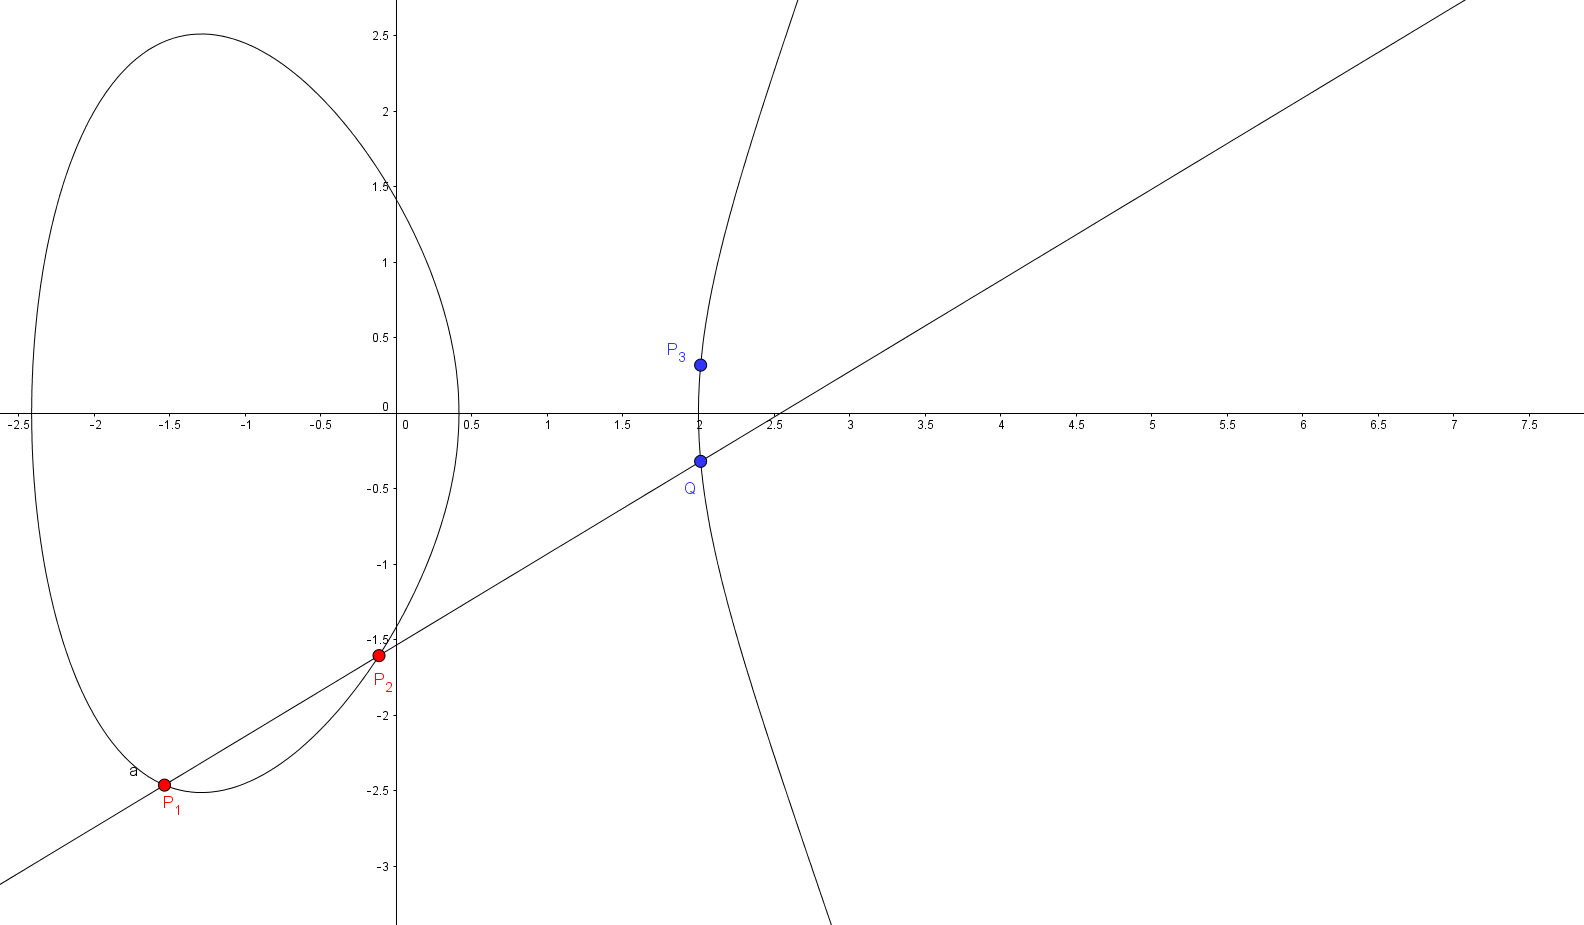
\includegraphics[width=0.8\linewidth]{lezione-161207-fig1}
\end{center}

\begin{proposizione}
La funzione $*$ appena definita è una legge di gruppo commutativa.
\end{proposizione}
\begin{proof}
La commutatività è ovvia.
L'elemento neutro è il punto all'infinito (si vede per ragioni geometriche).
L'inverso di $P = (x_1, y_1)$ è $-P = (x_1, -y_1)$, ovvero il simmetrico rispetto all'asse $x$.
Il vero osso duro è l'associatività, che in questo corso non dimostriamo.
\end{proof}

\begin{osservazione}
Se sappiamo che la cubica proviene da un toro, possiamo dire che la legge di gruppo $*$ proviene dal $+$ del toro (sotto quali ipotesi valgono sti sollevamenti mi sfugge). In questo modo anche l'associatività diventa ovvia.
\end{osservazione}

\section{Equivalenza lineare tra divisori (sulle cubiche)}

\begin{definizione}
Definiamo il gruppo dei divisori sulla cubica $\Div(\widetilde{E})$ come il gruppo abeliano libero generato dai punti della cubica. Per gli analisti, me compresa, significa che è l'insieme delle combinazioni formali finite del tipo $$\sum_{P \in \widetilde{E}} \alpha_P(P)$$,
con $\alpha_P \in \mathbb{Z}$.
Sempre per gli analisti: coraggio ragazzi, mancano poche lezioni!
RIP per questi commenti che verranno cancellati da Balbo, stima per lui se invece li lascia.
% Vabbè li lasciamo anche se sarebbe meglio di no. Balbo
Attenzione: anche la stringa vuota ($\alpha_P=0$ $\forall P$) è un elemento, in particolare è l'elemento neutro.
Equivalentemente posso pensarle come le funzioni dalla cubica in $\mathbb{Z}$ a supporto finito.
\end{definizione}

\begin{definizione}
Si definisce grado di un divisore il numero $\sum \alpha_P \in \mathbb{Z}$.
\end{definizione} 

\begin{osservazione}Il grado è un omomorfismo di gruppi $\deg: \Div(\widetilde{E}) \rightarrow \mathbb{Z}$.
\end{osservazione}

\begin{definizione}
Si definisce gruppo dei divisori di grado zero sulla cubica $\Div^0(\widetilde{E}) := \Ker(\deg)$.
\end{definizione}

\begin{definizione}
Per questa definizione supponiamo di sapere che la cubica viene da un toro.
Considero una funzione $f$ razionale non nulla su $\widetilde{E}$, cioè $f \in \bbC(\wp(z),\wp'(z))$. So che ha finiti zeri e finiti poli.
Si definisce: $\div(f) = \sum_{P\in T} \ord_P(f) \cdot (P) \in \Div(\widetilde E)$.
L'insieme di tutti i possibili $\div(f)$ si chiama insieme dei divisori principali.
\end{definizione}
\notamargine{Possiamo comunque definire, anche nel caso in cui la cubica non venga da un toro, il grado di una funzione razionale $f: \widetilde{E} \rar \bbC$. Preso un punto $p \in \widetilde{E}$ si può infatti considerare l'anello $\cO_{X, p} = \{ g: \widetilde{E} \rar \bbC \mid \mbox{razionali e definite in } p \}$, che risulta essere un DVR (è infatti locale e noetheriano, di dimensione uno, con ideale massimale principale) con ideale massimale $\cM_p$ delle funzioni razionali definite in $p$ che si annullano in $p$.

  A questo punto, visto che $f(p) = 0$ sappiamo che $f \in \cM_p^k$ per qualche $k \in \bbN$. Si definisce $\ord_p(f) = k$ (nel caso in cui $f$ abbia un polo in $p$ si definisce $\ord_p(f) = - \ord_p(\frac{1}{f})$).}

Un teorema che abbiamo visto (T2 sulle superfici di riemann compatte) garantisce che $\div(f) \in \Div^0(\widetilde{E})$
Inoltre $\{\div(f) | f: \widetilde{E} \rar \bbC \mbox{ razionale} \}$ è un sottogruppo di $\Div^0(\widetilde{E})$ (le verifiche sono banali).

C'è dunque un omomorfismo (non surgettivo) tra il gruppo moltiplicativo delle funzioni razionali non nulle su $\widetilde{E}$ e i divisori di grado zero.
$\varrho: \bbC(\widetilde E)^* \rightarrow \Div^0(\widetilde{E})$. Infatti $\div(fg)=\div(f)+\div(g)$.

\begin{proposizione}
$\Ker(\varrho) = \{\text{le funzioni costanti diverse da zero}\}$
\end{proposizione}
\begin{proof}
Un'inclusione ($\supseteq$) è banale, per l'altra possiamo osservare che se $\varrho(g)$ va nell'elemento
neutro di $\Div^0(\widetilde{E})$ (la stringa vuota), allora essa non ha né poli né zeri (neanche all'infinito), ma allora è necessariamente costante.
\end{proof}

\begin{osservazione}
Quindi ho una successione esatta che comincia così:
$$0 \rightarrow \bbC^* \rightarrow \bbC(\widetilde{E})^* \rightarrow \Div^0(\widetilde{E})$$
\end{osservazione}


\section{Divisori in un caso più semplice: $\bbP_1$}
$\bbC(\bbP_1) = \bbC(t)$ con $t$ che è la funzione coordinata $t(x_1, x_0)=\frac{x_1}{x_0}$.
Ha un polo nel punto all'infinito, cioè in $(1:0)$.

\begin{proposizione}
Ogni divisore di grado $0$ è il divisore di una funzione (nel caso di $\bbP_1$! Per $\widetilde E$ è falso.)
\end{proposizione}
\begin{proof}
  Possiamo supporre che $\infty$ non compaia nel divisore di grado $0$.
  Infatti, se per caso ci compare con coefficiente $n$, sarà sufficiente moltiplicare $f$ per la funzione $z^{-n}$ (in coordinate standard), che notiamo avere $\div z^{-n} = -n (0) + n (\infty)$, ovvero $z^{-n} \in \Ker \varrho$. E quindi $f \in \Ker \varrho \sse z^{-n} f \in \Ker \varrho$.
Allora (col piccolo abuso di identificare $\bbP_1 \backslash \infty$ con $\bbC$)
questo divisore sarà $\sum m_i (\alpha_i)$ con $m_i \in \mathbb{Z}$ e $\alpha_i \in \bbC$, e so che $\sum m_i=0$.
Calo dal cielo $\prod(t-\alpha_i)^m_i$, e si vede facilmente che risolve.
\end{proof}
\notamargine{La cosa che stiamo facendo è semplicemente di richiamare il classico teorema che ogni funzione meromorfa sulla sfera di Riemann si legge nelle carte standard come funzione razionale (con stesso grado sopra e sotto la linea di frazione)}

\section{Torniamo sulle cubiche: il gruppo di Picard}
In generale possiamo definire:

\begin{definizione}
$\Pic^0(\widetilde{E}) := \frac{\Div^0(\widetilde{E})}{\text{divisori principali}}$
\end{definizione}

\begin{osservazione}
Ho quindi la successione esatta:
$$0 \rightarrow \bbC^* \rightarrow \bbC^*(\widetilde{E}^*) \rightarrow \Div^0(\widetilde{E})\rightarrow \Pic^0(\widetilde{E})\rightarrow 0$$
\end{osservazione}

Nel caso visto prima di $\bbP_1$, già $\Pic^0(\bbP_1)=0$

\notamargine{
Avere il $\Pic=0$ è imparentato in qualche modo con l'essere UFD. Ad esempio $\mathbb{Z}(i)$ ha $\Pic=0$. Nel caso del $\bbP_1$, il fatto che il suo $\Pic$ sia nullo è dunque legato alla fattorizzazione unica dei polinomi.
}

\section{Vogliamo ora studiare il Pic di una curva ellittica (proveniente da un toro)}

Considero $\sigma : \widetilde E \rightarrow \Div^0(\widetilde E)$ tale che $\sigma(P)=(P)-(0)$
Considero un divisore di grado $0$ su $E$. Sarà della forma $d = \sum\alpha_P\cdot(P)$.
Poiché $\sum \alpha_P=0$, lo posso scrivere come $\sum\alpha_p \sigma(P)$.

\begin{definizione}
Equivalenza lineare tra divisori. Si dice che $d_1 \sim d_2$ se $d_1-d_2$ è un divisore principale. Attenzione! Non tutti i divisori di grado zero sono principali.
\end{definizione}

\begin{teorema}
  \label{teorema_divisori_semplici}
Ogni divisore di grado zero è linearmente equivalente ad un $\sigma(P)$.
\end{teorema}

Alla dimostrazione premettiamo alcuni lemmi. 
\begin{lemma}
  \label{lemma_equiv_lin}
$(R) + (-R) \sim 2(0)$
\end{lemma}
\begin{proof}
Sia $R$ è il punto di $\widetilde E$ associato al punto $z_0 \in T$.
Dimostro ora che $(R)+(-R)-2(0)$ è un divisore principale, da cui $(R)+(-R)-2(0) \sim \varnothing$ da cui la tesi.
Ma considerando la funzione $\wp(z)-\wp(z_0)$ si vede che ha divisore $(R)+(-R)-2(0)$ (polo doppio in $0$, zeri semplici in $R,-R$), da cui la tesi.
\end{proof}

\begin{lemma}
  \label{lemma_equiv_lin2}
$\sigma(P)+\sigma(Q) \sim \sigma (P+Q)$
\end{lemma}
\begin{proof}
La tesi equivale a:
$$(P)-(0)+(Q)-(0) \sim (P+Q)-(0)$$
$$(P)+(Q)\sim (P+Q)+(0)$$
Attenzione: si intende che il $+$ dentro alle parentesi è la legge di gruppo sulla cubica indotta dall'addizione del toro, mentre il $+$ fuori dalla parentesi è il $+$ formale dei divisori.
Considero la funzione $h(z) = \wp'(z) - a \wp(z) - b$ con a e b definiti come nel Teorema \ref{leggedigruppo}. Abbiamo già visto che ha un polo di ordine $3$ nell'origine e tre zeri semplici in $P$, $Q$, $-P-Q$. Quindi $$\div(h)=(P)+(Q)+(-P-Q)-3(0) \sim \varnothing$$
Utilizzo ora il lemma \ref{lemma_equiv_lin}, e ottengo che:
$$(P)+(Q)+2(0)-(P+Q)-3(0) \sim \varnothing$$
$$(P)+(Q) \sim (P+Q)-(0)$$
\end{proof}

\begin{proof}[Dimostrazione del Teorema]
Considero un qualsiasi divisore $d$ di grado $0$.
$$d=\sum a_i (P_i)$$
per $i=1,...,n$. So che $\sum a_i=0$. Allora:
$$d = \sum a_i (P_i)-\sum a_i (0) \sim \sum a_i ((P_i)-(0))=\sum a_i (\sigma(P_i))$$
Ma adesso estendendo banalmente il lemma \ref{lemma_equiv_lin2} dalle somme alle combinazioni lineari, ottengo che:
$$d \sim \sum a_i (\sigma(P_i)) \sim \sigma(\sum a_i P_i)$$
da cui la tesi.
\end{proof}


\chapter{23 Gennaio 2017 - Biliardi ellittici e Funzioni Modulari}
\justify

\section{Biliardi ellittici}
\newthought{Introduciamo un altro modo} in cui si ottengono le curve
ellittiche dalle ellissi \notamargine{Abbiamo infatti già visto che si
  possono ottenere come integrali della lunghezza d'arco di un'ellisse}.

Prendiamo un'ellisse di equazione $ax^2 + by^2 = 1$ e supponiamo di
giocare a biliardo sull'ellisse: facendo partire la pallina da un punto
la lanciamo contro il bordo dell'ellisse su cui rimbalza secondo la nota
legge della riflessione \notamargine{Ovvero rispetto alla tangente
  all'ellisse nel punto rimbalza via con lo stesso angolo, come indicato
  in figura}

\begin{center}
  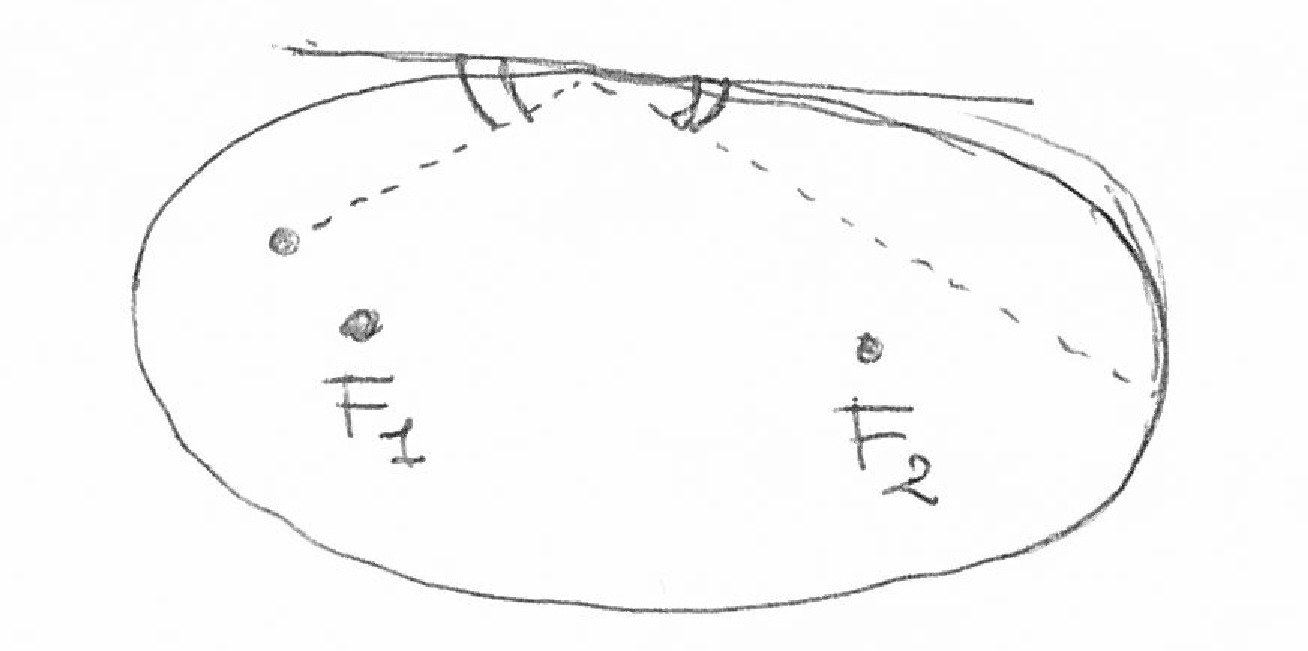
\includegraphics[width=8cm]{lezione-170123-fig1}
\end{center}
  
Una cosa che è nota da tempo è che le rette che compongono la
traiettoria sono tutte tangenti ad un'altra ellisse ``caustica'' che ha
gli stessi fuochi della prima: abbiamo quindi una famiglia ad un
parametro di ellissi che descrive tutte le possibili traiettorie.

\newthought{Vediamo allora che succede} quando prendiamo un punto $P$
sul bordo dell'ellisse ed una retta $l$ con $P \in l$ e tangente alla
caustica:

Possiamo definire un'applicazione $\phi$ dalle coppie punto-retta in sè
che è la funzione di ``evoluzione'' della traiettoria sul biliardo,
ovvero manda la coppia $(P, l)$ in $(P', l')$ con $P'$ l'altro punto di
intersezione della retta $l$ con l'ellisse e $l'$ la retta passante per
$P'$ che segue la legge della riflessione con $l$.

\notamargine{
  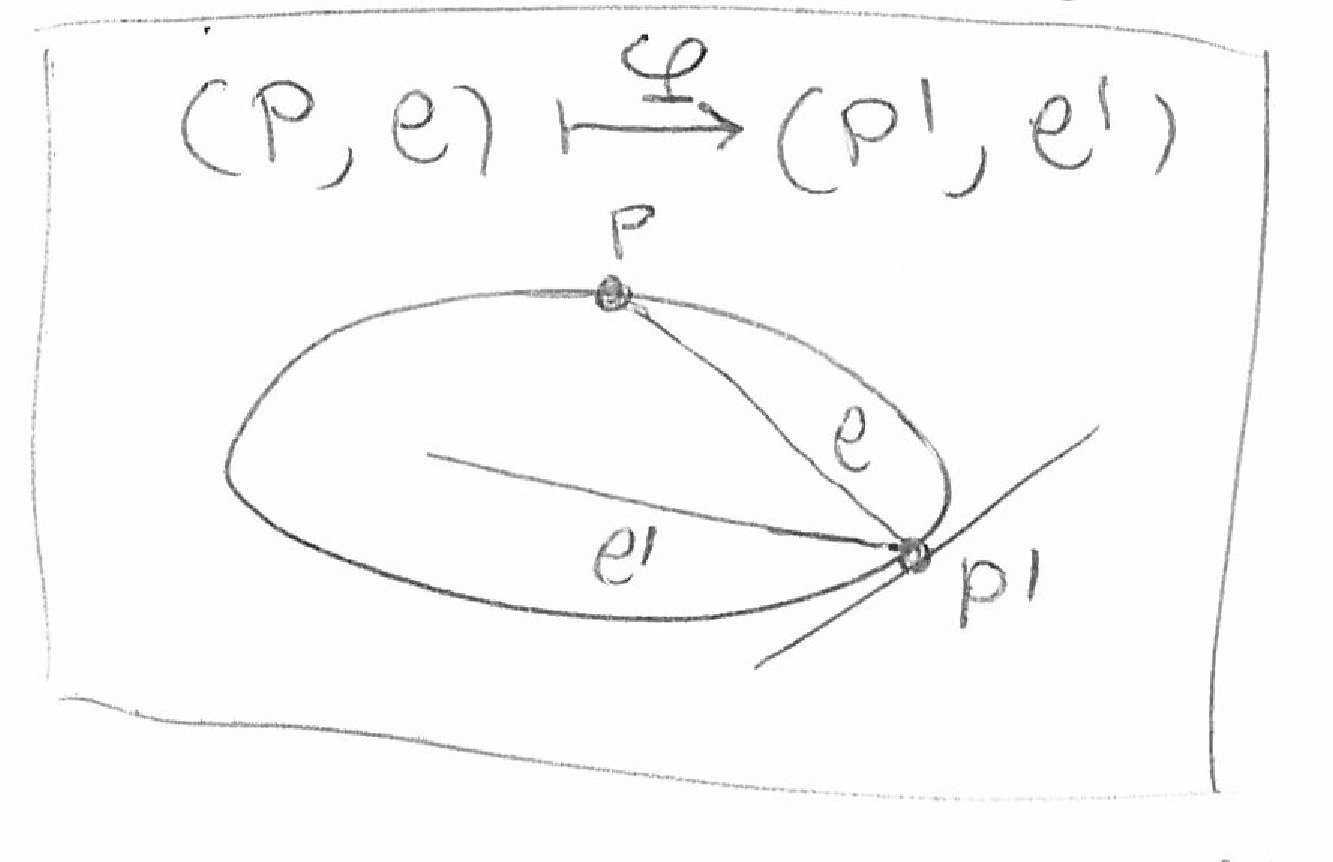
\includegraphics[width=4cm]{lezione-170123-fig2}
}

\newthought{È noto} che le tangenti in $\bbP^2$ ad una conica sono
parametrizzate da un'altra conica: la conica duale.
\notamargine{Tutto ciò non è difficile da verificare: se la conica $\cC$
  ha equazione $f = ax^2 + by^2 + cz^2$ e $(x_0, y_0, z_0) = P \in \cC$
  allora $(\nabla f)_P = (2ax_0, 2by_0, 2cz_0)$ e, ricordando che tutti
  i punti/vettori considerati sono in $\bbP^2$ si ha che dare la retta
  tangente in $P$ è uguale a fornire il vettore $(\nabla f)_P$. D'altra
  parte si riesce ovviamente a recuperare il punto $P$ dato $(\nabla
  f)_P$ a cui è tangente (basta vedere la formula scritta sopra in
  coordinate, visto che i coefficienti della conica sono noti)}
Allora il luogo di punti su cui la $\phi$ agisce è una sottovarietà
(algebrica) di $C_1 \times \hat{C_2}$, con $C_1 = \text{punti della
  conica}$ e $\hat{C_2} = \text{conica duale delle rette tangenti}$.

Il luogo di punti è dato dalle coppie $(P, l) \in C_1 \times \hat{C_2}$
tali che $P \in l$ (che è una condizione chiusa, ovvero dà luogo ad una
sottovarietà algebrica). Questa è anche una superficie di Riemann.

Scrivendo l'equazione si ottiene una curva ellittica e l'operazione
$\phi$ si rivela essere una traslazione sulla cubica detta ``gioco di
Poncelèt''.

Il gioco ``finisce'' se e solo se la traslazione $\phi(x) = x + \tau$ ha
un punto di ordine finito, ovvero $\exists n$
$\phi^n (x) = x + n\tau = x$ se e solo se $n\tau \in L$, il
reticolo. Ovvero si avrebbe $\phi^n(x) = x$ per ogni punto. Allora se il
gioco finisce per una traiettoria finisce per tutte le altre, cosa che
non è per nulla banale.

\notamargine{Come curiosità, se il gioco non finisce, le traiettorie del
  biliardo sono dense nello spazio tra le due caustiche}

\section{Funzioni Modulari}

\notamargine{Il nome ``modulari'' è riferito ai moduli, parametri che
  comparivano negli integrali ellittici. Oggi ci si riferisce a moduli
  per indicare uno spazio di parametri per una famiglia di curve
  algebriche.

  Esempio ``stupido'': $y - a x^2 = 0$ al variare di $a \in \bbC$ sono
  una famiglia di parabole (o per $a=0$ una retta). In questo caso lo
  spazio dei parametri è $\bbC$ (nel quale $a$ può variare)}

\begin{osservazione}
  Ricordiamo che conosciamo già un parametro delle cubiche:
  $j$. Infatti, se la cubica viene da un toro allora è della forma
  $y^2 = 4 x^3 - g_2 x - g_3$ e sappiamo che
  $j = 1728 \frac{g_2^3}{g_2^3 - 27 g_3^2}$ è un'invariante per
  trasformazioni algebriche delle cubiche.
\end{osservazione}

Siamo allora autorizzati a riscalare il reticolo $L$ pur restando nella
stessa classe di isomorfismo delle cubiche. Possiamo quindi supporre che
$L = \bbZ \tau + \bbZ 1$ con $\tau \in \cH = \{ z \in \bbC | \Img \tau >
0 \}$. In questo modo $g_2 = 60 \sum_{\omega \in L^*} \omega^{-4}$ e
$g_3 = 140 \sum_{\omega \in L^*} \omega^{-6}$ diventano funzioni
olomorfe di $\tau$ come parametro nel semipiano superiore e quindi pure
$j$ è una funzione di $\tau$

\begin{osservazione}
  Se vedessimo che $j$ assume tutti i valori in $\bbC$ ciò dimostrerebbe
  che tutte le cubiche provengono da un toro, poiché sappiamo già che
  due cubiche sono affinemente equivalenti se e solo se hanno lo stesso $j$.
\end{osservazione}

\begin{divagazione}
  Si può dimostrare che $\tau$ è immaginario quadratico su $\bbQ$ allora
  $j(\tau)$ è un numero algebrico. Di seguito diamo un'idea della dimostrazione
  \notamargine{ Immaginario quadratico vuol dire che soddisfa
    un'equazione di secondo grado a coefficienti in $\bbQ$, ovvero $x$ è
    tale che $\exists b, c \in \bbQ$ con $x^2 + bx + c = 0$}

  Quando $\tau$ è un immaginario quadratico il reticolo ha infatti degli
  automorfismi non banali. Se $j$ fosse trascendente, visto che gli
  automorfismi sono funzioni razionali delle coordinate e avremmo
  $\bbQ(j, \text{funz.raz.})$ come campo finitamente generato su $\bbQ$,
  che ha grado di trascendenza uno.

  Allora si può ``specializzare'' $j$, visto che il campo è isomorfo ad
  una cosa con una variabile.

  \notamargine{Qui intendiamo ad esempio che $\bbQ(j, \sqrt{j + 2})
    \cong \bbQ(t, \sqrt{t + 2})$ con $t$ come variabile e quindi $\cong
    \bbQ(t_0, \sqrt{t_0 + 2})$ con $t_0$ trascendente.}
  
  Specializzandolo ad ogni altro numero trascendente ottengo un campo
  isomorfo e quindi tutte le curve ellittiche avrebbero degli
  automorfismi non banali (poiché hanno uguali campi) e ciò è
  impossibile poiché le cubiche con automorfismi sono in numero
  numerabile.
\end{divagazione}

Il reticolo $L$ può avere altre basi, date dall'applicazione di matrici
$\kM_{2 \times 2} (\bbZ)$ invertibili. Possiamo scegliere l'ordine dei
due elementi della base in modo da avere soltanto le matrici con
determinante uno.

Diciamo che due reticoli $\bbZ + \bbZ \tau = \bbZ + \bbZ \tau'$ sono
equivalenti se $\exists g \in \SL_2 \bbZ$
$\tc g\tau = \tau' = \frac{a \tau + b}{c \tau + d}$

Allora i tori complessi modulo isomorfismo sono in biggezione con $\cH$
modulo $\SL_2 \bbZ$ (in realtà l'azione si quozienta per $\{\pm 1\}$,
quindi l'azione è di $\bbP\SL_2 \bbZ$).

\section{Costruzione di un dominio fondamentale}

Vogliamo costruire un dominio fondamentale per lo spazio dei reticoli,
ovvero su cui agiranno le funzioni modulari.
\notamargine{Per dominio fondamentale intendiamo uno spazio in cui è
  presente esattamente un rappresentante per ogni reticolo. Nel nostro
  caso portiamo ogni reticolo nella forma $L = \bbZ + \bbZ \tau$}

Descriviamo innanzitutto la forma del dominio fondamentale:
$ F = \cH \cap \{ \Re z \in [ -\frac{1}{2}, \frac{1}{2} ) \} $
tolto l'insieme $\{ \abs{z} < 1 \} \cup \{ \abs{z} = 1 \mid \Re z > 0 \}$

e definiamo le due applicazioni
$$ S = \lbr{\begin{array}{cc} 0 & 1 \\ -1 & 0 \\ \end{array}} $$
$$ T = \lbr{\begin{array}{cc} 1 & 1 \\ 0 & 1 \\ \end{array}} $$
tra cui si hanno le relazioni $S^2 = (TS)^3 = \Id$

\begin{center}
  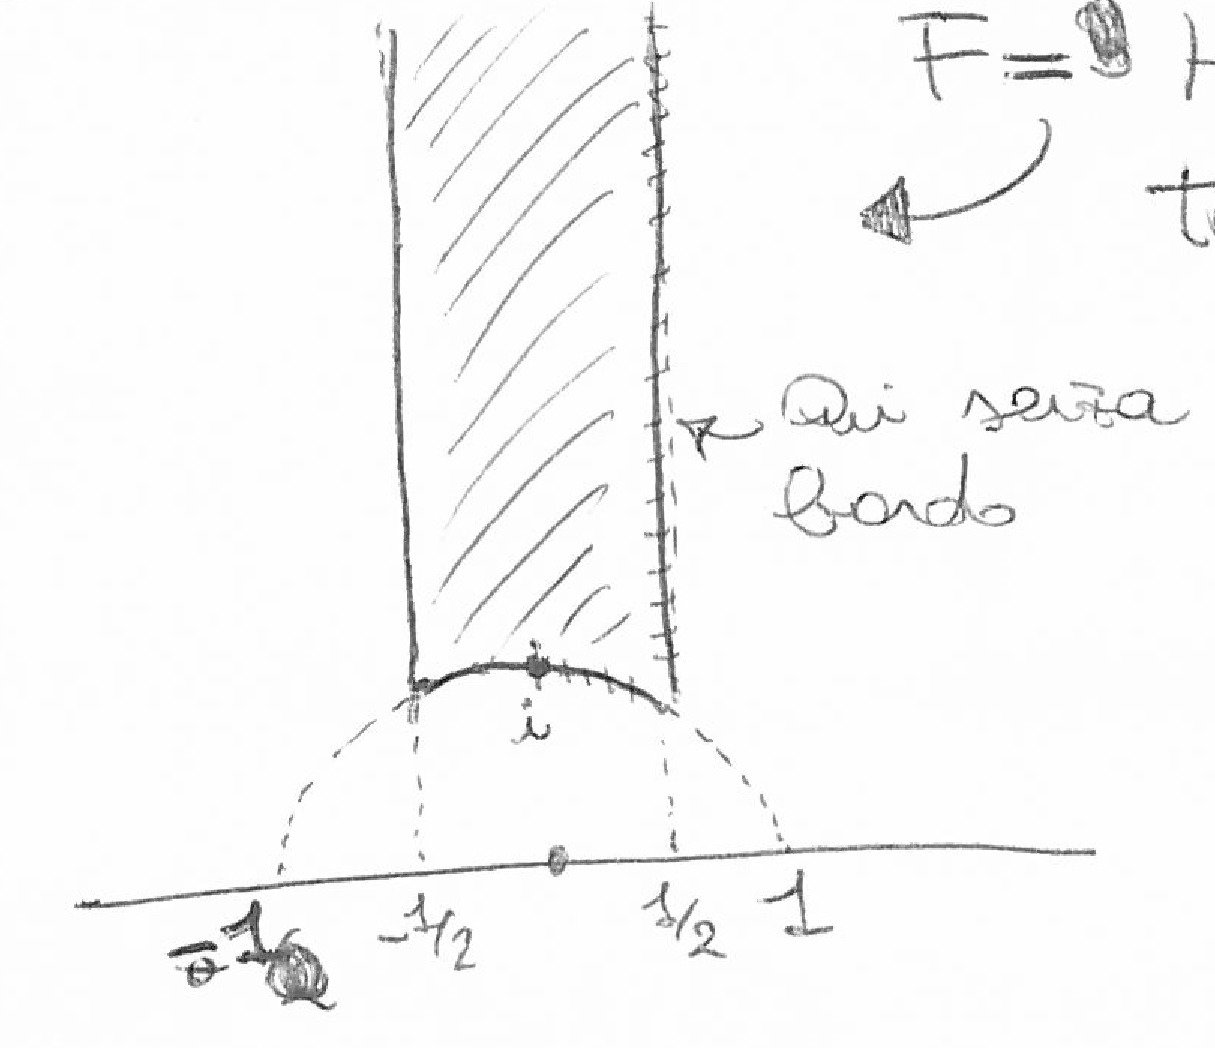
\includegraphics[width=8cm]{lezione-170123-fig3}
\end{center}

\begin{osservazione}
  Sarà parecchio importante sapere che se
  $g = \lbr{\begin{array}{cc} a & b \\ c & d \\ \end{array}} \in
  \SL_2(\bbZ)$, allora si ha $\Im (gz) = \frac{\Im z}{\abs{cz + d}^2}$.
\end{osservazione}

\begin{lemma}
  $\SL_2 \bbZ$ è un sottogruppo discreto come sottoinsieme di $\SL_2 \bbR$
  ed agisce in modo propriamente discontinuo su $\cH$
\end{lemma}
\begin{proof}
  Sia $K \subseteq \cH$ un compatto: vogliamo mostrare che allora
  $gK \cap K \neq \emptyset$ per al più un numero finito di $g \in G$.

  Allora sia $z_0 \in K$ tale che $g z_0 \in K$. Sappiamo però che per
  un qualunque compatto in $\cH$ $\exists \rho, \rho'$ che dipendono
  solo dal compatto tali che $\rho' > \Im z > \rho > 0$ per un qualunque
  $z \in K$. Se anche $g z_0 \in K$ ne segue allora che $\abs{cz_0 + d}$
  è limitato uniformemente in $z_0$ $\implies$
  $\Im (cz_0 + d) = c \Im z_0$ $\implies$ $c$ è limitato ed anche $d$ è
  limitato (e la limitazione dipende solo da $K$)

  $\frac{a z_0 + b}{c z_0 + d} \in K$. Allora, visto che le possibili
  coppie $(c, d)$ sono finite, si ha
  $a z_0 + b \in \cup_{(c, d)} (cK + d)K$ che è compatto e quindi si
  conclude come sopra (utilizzando $\rho$ e $\rho'$)
\end{proof}

Anche se l'azione è propriamente discontinua il quoziente non è comunque
rivestito perché ci sono dei punti fissi: ad esempio $Si = i$ e $TS
\zeta_3 = \zeta_3$. Ma sono gli unici due punti che danno fastidio.

\notamargine{Incollando i bordi del dominio fondamentale si può vedere
  che topologicamente lo spazio delle curve ellittiche è omeomorfo a
  $\bbC$, anche se ovviamente non può esserne biolomorfo né rivestito
  per le conseguenze del teorema di classificazione di Riemann}

Nella prossima lezione vedremo il teorema che ci mostra che $F$ come
descritto è effettivamente un dominio fondamentale e, come curiosità:
\begin{teorema}
  $G = \SL_2 \bbZ$ è generato da $S$ e da $T$. Inoltre è esattamente il
  gruppo libero su due elementi ($S$ e $T$) con le relazioni
  $S^2 = (TS)^3 = \Id$
\end{teorema}


\thislesson{31 Gennaio 2017}{Azione di $SL_2 \left( \bbZ \right)$ su $\cH$ e Funzioni Modulari}

\section{Azione di $SL_2 \left( \bbZ \right)$ su $\cH$}

Siano $F=\left\{z \in \cH | -\frac{1}{2} \leq \Re(z) \leq 0
\wedge |z| \geq 1 \right\} \cup
\left\{z \in \cH | 0 < \Re(z) < \frac{1}{2} \wedge |z| > 1 \right\}$,
$G=SL_2 \left( \bbZ \right)/\{\pm Id\}$,   $\rho=\frac{-1+i\sqrt{3}}{2}$,
$S=\left( \begin{array}{cc} 0 & 1 \\ -1 & 0 \end{array} \right) \in G$,
$T=\left( \begin{array}{cc} 1 & 1 \\ 0 & 1 \end{array} \right) \in G$,
$G' = \langle S, T \rangle$.

\begin{teorema}
\begin{itemize}
\item[P0] $\forall z \in \cH \quad \exists g \in G$ tale che $gz \in F$
\item[P1] se $z,gz \in \bar{F}$ con $g \neq \Id$, allora $z \in \partial F$.
  Più precisamente si hanno i tre casi (anche se non disgiunti):
  \begin{enumerate}
  \item[C1] $\Re z = \pm \frac{1}{2}$ e $z' = z \mp 1$
  \item[C2] $|z| = 1$ e $z' = - \frac{1}{z}$
  \item[C3] $z = z' = \rho$ oppure $z = z' = \rho + 1$
  \end{enumerate}
\item[P2] se $z \in F$ e $z=gz$,
  allora $z=i$ (nel qual caso $g \in \left\langle S \right\rangle$) oppure si ha che
  $z= \rho$ (nel qual caso $g \in \left\langle ST \right\rangle$)
\end{itemize}
\end{teorema}

\begin{proof}
  \squared{P0}
Sia $G'=\left\langle S,T \right\rangle$. Sia $z \in \cH$ e cerchiamo $z' \in G'z$ con $\Im(z')$ massima possibile. Tale elemento esiste, infatti se
$\sigma = \left( \begin{array}{cc} a & b \\ c & d \end{array} \right) \in G'$, allora $\Im(\sigma z) = \frac{\Im(z)}{|cz+d|^2}$ ed essendo
$c,d \in \bbZ$, $|cz+d|^2 \geq (\Im(z))^2$ (per $c \neq 0$, se no fa $d^2 \ge 1$) per cui $\Im(\sigma z)$ è limitato dall'alto e il sup viene raggiunto perché
ci sono solo un numero finito di $c,d \in \bbZ$ per cui $|cz+d|^2 \leq 1$. (Infatti siccome lo cerco massimo voglio denominatore più piccolo di uno,
altrimenti già $z$ andava bene)

\notamargine{Per vedere che ve ne sono un numero finito scriviamo $|cz+d|^2 = c^2 (\Im z)^2 + (c \Re z + d)^2 \le 1$.
  Allora ciascun termine è minore di $1$, quindi ci sono un numero finito di $c$, e da questo si ricava che vi sono un numero finito di $d$.}

Possiamo quindi supporre che $z=z'$ e, a meno di comporre con qualche potenza
di $T$ (che è una traslazione), supponiamo anche che $-\frac{1}{2} \leq \Re(z) < \frac{1}{2}$.

Verifichiamo quindi che $|z| \geq 1$ (se poi fosse $|z|=1$ e
$z \in \bar{F} \setminus F$ basta applicarci $S$).
$\frac{\Im(z)}{|z|^2} = \Im(Sz) \leq \Im(z)$ per la massimalità di $\Im(z)$.
Quindi $|z| \geq 1$.
\vskip 0.5cm

\squared{P1}
Siano ora $g \in G$, $z'=gz$ e supponiamo che $z,z' \in \bar{F}$ e (wlog)
che $\Im(z) \leq \Im(z')$.
$$
z'= gz \cdot 1 = \frac{az+b}{cz+d} \frac{c \bar{z} +d}{c \bar{z} +d} =
\frac{ac|z|^2 + bd + bc \bar{z} + adz}{|cz+d|^2} \stackrel{det=1}{=}
\frac{ac|z|^2 + bd + bc \bar{z} + (bc+1)z}{|cz+d|^2} =
$$
$$
\frac{ac|z|^2 + bd + bc (\bar{z} + z) + z}{|cz+d|^2} =
\frac{ac|z|^2 + bd + (2bc+1) \Re(z)}{|cz+d|^2} + i \frac{\Im(z)}{|cz+d|^2}
$$
Ora, usando che $z,z' \in \bar{F}$, per cui $|z|,|z'| \geq 1$ e
$|\Re(z)|, |\Re(z')| \leq \frac{1}{2}$, si ottiene che, se $c \neq 0$,
$\Im(z') = \frac{\Im(z)}{|cz+d|^2} \leq \frac{\Im(z)}{c^2 \Im(z)^2}
= \frac{1}{c^2 \Im(z)} \leq \frac{2}{c^2 \sqrt{3}}$ $\implies c^2 \le \frac{2}{\sqrt{3}\Im z'} \le \frac{4}{3}$
quindi $|c| \leq 1$.

\begin{itemize}
\item Se $c=0$, allora (visto che $ad - bc = 1$) deve essere $z' = z \pm b$, per cui si può avere $z'=z$ e $g=Id$; oppure
  $|\Re(z')| = \frac{1}{2}$ e $|\Re(z)| = -\frac{1}{2}$; o viceversa.
  \notamargine{Nel caso $c=0$ stando $z, z' \in F$ si ha $|\Re z - \Re z'| \le 1$}
  Negli ultimi due casi si ha $z,z' \in \partial F$ e $g=T$ e vale C1.

\item Se invece $c=1$ (il caso $c=-1$ è uguale perché
  $G=SL_2 \left( \bbZ \right)/\{\pm Id\}$),
  $\Im(z') \leq \frac{1}{\Im(z)} \stackrel{z' \in F}{\Rightarrow} \Im(z) \leq \frac{2}{\sqrt{3}}$.
  Allora $\Im(z') \leq \frac{2}{\sqrt{3}|z+d|^2} \Rightarrow
  |z+d|^2 \leq \frac{4}{3} \Rightarrow |z|^2+d^2+2d \Re(z) \leq \frac{4}{3}$. 
  Quindi (poiché $\Re z \ge -\frac{1}{2}$) $d=0$ o $d=\pm 1$.

  Se $d=0$, $\Im(z') = \frac{\Im(z)}{|z|^2} \leq \Im(z)$, quindi $|z|=1$ (Perché avevamo precedentemente assunto che $\Im(z) \le \Im(z')$).
  Considerando il determinante si ottiene $b = -1$ e quindi $z' = \frac{az - 1}{z} = a - \frac{1}{z} = a - \bar{z}$. Siccome $z$ è sulla circonferenza unitaria anche $- \bar{z}$ lo è; visto che sia $z'$ che $z$ devono stare in $F$, deve essere $a = 0, \pm 1$.
  \begin{itemize}
  \item $a = 0$. Allora siamo nel caso C2
  \item $a = \pm 1$ allora $z = z' \in \{\rho, \rho + 1\}$ e siamo nel caso C3
  \end{itemize}

  Se $d=\pm 1$, similmente $\Im(z') = \frac{\Im(z)}{|z \pm 1|^2}$. Usando che $|z \pm 1| \ge 1$ (Fare disegno e cercare minimo modulo di $F + 1$)
  si ottiene $|z \pm 1|=1$, da cui, di nuovo, $z=\rho, z'=\rho + 1$ o viceversa e siamo nel caso C1.
\end{itemize}

\bigskip
\squared{P2} Utilizzando il punto P1 distinguiamo i tre casi:
\begin{itemize}
\item Il caso C1 non si realizza perché avevamo $z' \neq z$
\item Il caso C2 ci da $z^2 = -1 \implies z = i$ e, per quanto visto sopra, si ha $g = S$
\item Il caso C3 ci da solo $z = z' = \rho$ perché $\rho + 1 \notin F$ e si ottiene $g = \left(\begin{array}{cc} -1 & -1 \\ 1 & 0 \\ \end{array} \right) = (ST)^2$, quindi (visto che $(ST)^3 = \Id$) lo stabilizzatore è il sottogruppo $\langle ST \rangle$
\end{itemize}
\end{proof}

\begin{corollario}
F è un dominio fondamentale.

$Stab(i)=\left\langle S \right\rangle$, 
$Stab(\rho)=\left\langle ST \right\rangle$ e $Stab(z)=\emptyset$ se 
$z \notin \{i, \rho \}$.
\end{corollario}

\begin{teorema}
G è generato da S e T
\end{teorema}

\notamargine{In realtà si potrebbe dimostrare anche che G è il gruppo libero
generato da $S$ e $T$ modulo le relazioni $S^2=Id$ e $(TS)^3=Id$}

\begin{proof}
Vediamo ora che $G'=G$:

Sia $z=2i$ e sia $g \in G$. Per quanto visto sopra, $\exists \sigma \in G'$
tale che $\sigma g(z) \in \bar{F}$. Allora, dato che $z \notin \partial F$,
$\sigma g(z)=z$.
Poiché gli unici stabilizzatori non banali sono quelli
previsti dal corollario, ne deduciamo che $\sigma g = Id$ e quindi $G=G'$.
\end{proof}

\begin{osservazione}
  Al quoziente $\cH/G \simeq F$ si può dare una struttura di superficie di Riemann
  (che non è quella data dall'immersione per via dei due stabilizzatori non banali),
  identificando le rette $\Re(z)=\pm \frac{1}{2}$ e i due archi di circonferenza
  (quelli passanti per $i$) sul bordo di $F$. Il quoziente è omeomorfo a $\bbC$.
  Possiamo quindi indurre una struttura di superficie di Riemann con l'omemomorfismo trovato.
\end{osservazione}

\section{Forme quadratiche binarie intere}
Una forma quadratica binaria intera è un'espressione del tipo:
$$ ax^2+bxy+cy^2 \qquad a,b,c,d \in \bbZ $$
Si vogliono classificare a meno di equivalenza lineare con elementi di
$SL_2 \left( \bbZ \right)$.

\begin{osservazione}
Il discriminante $\Delta =b^2-4ac$ è invariante per trasformazioni lineari
invertibili. Inoltre, fissato $\Delta$, il numero di classi di equivalenza con
quel discriminante è FINITO (questo però è difficile).
Quando $\Delta < 0$, è utile considerare $\xi \in \cH$ che risolve
$a \xi^2 + b \xi + c =0$. Per quanto abbiamo visto, $\exists \sigma \in G$
tale che $\sigma \xi \in F$. Tramite $\sigma$ si ottiene la forma ridotta secondo
Gauss.
\end{osservazione}

\section{Funzioni Modulari}
\begin{definizione}
Una funzione $f$ meromorfa su $\cH$ di dice debolmente modulare di peso $2k$ (per $k \in \mathbb{N}$), se $\forall
\left( \begin{array}{cc} a & b \\ c & d \end{array} \right) \in
SL_2 \left( \bbZ \right)$ si ha:
$$ f\left( \frac{az+b}{cz+d} \right) = (cz+d)^{2k} f(z)
\qquad \forall z \in \bbC$$
\end{definizione}

\begin{osservazione}
$\displaystyle{gz=\frac{az+b}{cz+d} \stackrel{\det = 1}{\Rightarrow}
\frac{d(gz)}{dz}=\frac{1}{(cz+d)^2}}$. Quindi la condizione della definizione di
funzione debolmente modulare può essere scritta come $f(gz)(d(gz))^k=f(z)(dz)^k$.
Sono k-forme differenziali (secondo noi però sono tensori $(0, k)$ simmetrici).
\end{osservazione}

\begin{osservazione}
Dalla definizione segue immediatamente che $f(z+1)=f(z)$, cioè che una
funzione debolmente modulare è periodica di periodo $1$. Definendo $q(z) = e^{2 \pi i z}$
si ha che $q$ manda $\cH$ in $D^*$ (e in particolare $\cH / \bbZ \simeq D^*$), quindi
$\widetilde{f} = f \circ q^{-1}$ è meromorfa in $D^*$ e
$\displaystyle{\sum^{+\infty}_{n=-\infty}{a_n q^n}}$ è la sua serie di Laurent.
Quindi $f$ si può scrivere in ``serie di Fourier'' in $q=e^{2 \pi i z}$, cioè
$\displaystyle{f(z)=\widetilde{f}(q)=\sum^{+\infty}_{n=-\infty}{a_n q^n}}$.
\end{osservazione}
\notamargine{Non capiamo bene come si possa dedurre la sviluppabilità in serie di Laurent
  (i poli potrebbero accumularsi in $0$). Si può invece ben fare se $f$ è una funzione modulare,
  definita poco più sotto.}

\begin{definizione}
Nelle notazioni di sopra, se $\widetilde{f}$ è meromorfa anche in $D$, cioè
se gli $a_n$ con indice $n<0$ non nulli sono in numero finito, la $f$
è "meromorfa all'$\infty$" e si dice {\bf funzione modulare}.

Se poi $\widetilde{f}$ è olomorfa su tutto $D$ ($0$ compreso), cioè se tutti gli $a_n$ con $n<0$
sono nulli, la $f$ è "olomorfa all'$\infty$" e si dice {\bf forma modulare}.

Infine, se anche $a_0=0$, cioè $f(\infty)=0$, $f$ si dice forma modulare
cuspidale
\end{definizione}

\section{Esempio: Le Serie di Eisenstein}

\begin{definizione}
Se $L$ è un reticolo in $\bbC$, per $k \geq 2$ poniamo
$G_k(L):=\displaystyle{\sum_{\lambda \in L \setminus \{ 0 \}}{\lambda ^{-2k}}}$.
\end{definizione}

\begin{osservazione}
Proprietà di $G_k$:

\begin{itemize}
\item Le $G_k$ sono $(-2k)$-omogenee, cioè
$L_1=cL_2 \Rightarrow G_k(L_1)=c^{-2k}G_k(L_2)$.
Scrivendo $L=\bbZ \tau + \bbZ$, con $\tau \in \cH$,
si può anche vedere $G_k(L) = G_k(\tau)$ come funzione su $\cH$.
In questo modo, $\displaystyle{G_k(z)=\sum_{(m,n) \in \bbZ^2 \setminus
(0,0)}{\frac{1}{(mz+n)^{2k}}}}$, che converge uniformemente sui compatti
di $\cH$.
\item $G_k(z)$ converge puntualmente su $\cH$ e su $-\cH$, ma non su tutto $\bbC$. Infatti se $z \in \mathbb{R}$ i denominatori possono
essere arbitrariamente vicini a $0$ e quindi la serie diverge.
\item Ricordando la definizione di $g_2$ e $g_3$ si ha: $g_2(z)=60G_2(z)$ e $g_3(z)=140G_3(z)$.
\item Se $\left( \begin{array}{cc} a & b \\ c & d \end{array} \right) \in
SL_2 \left( \bbZ \right)$,
$\displaystyle{ G_k \left(\frac{az+b}{cz+d} \right) = 
\sum_{(m,n) \in \bbZ^2 \setminus (0,0)}
{\frac{(cz+d)^{2k}} {(m(az+b)+n(cz+d))^{2k}}} =}$
$\displaystyle{ =(cz+d)^{2k} \sum_{m,n}{\frac{1} {(m(az+b)+n(cz+d))^{2k}}} =
(cz+d)^{2k} \sum_{m,n}{\frac{1}{(mz+n)^{2k}}} }$, perché
$SL_2 \left( \bbZ \right)$ lascia invariati i reticoli. Quindi $G_k$
è debolmente modulare.
\end{itemize}
\end{osservazione}


\begin{proposizione}
Le $G_k$ sono forme modulari.
\end{proposizione}

\begin{proof}
Sono tutte olomorfe su $\cH$ per teoremi classici di convergenza.
Se $G_k$ avesse un polo o un sigolarità essenziale all'$\infty$, ci sarebbero
delle successioni $\{ z_n \} \subset \cH$ tali che
$|z_n| \rightarrow +\infty$ e $|G_k(z_n)| \rightarrow +\infty$.
Ma $\displaystyle{\lim_{\Im(z) \rightarrow +\infty} G_k(z)=
2 \sum_{n=1}^{+\infty}{\frac{1}{n^{2k}}} = 2 \zeta(2k)}$, perché i termini
con $m \neq 0$ vanno a $0$ uniformemente. Quindi le $G_k$ sono olomorfe
all'$\infty$.
\end{proof}

\begin{osservazione}
$\Delta = g_2 ^3 (z) - 27 g_3 ^2 (z)$ è una forma modulare di peso $12$ che
non si annulla mai in $\cH$.
\end{osservazione}
\end{document}

